\documentclass[
    BCOR=6mm,
    DIV=13,
    draft=false,
    titlepage=true,
    twoside=false,
    toc=bib,
    parskip=half-,
    chapterprefix=true,
    appendixprefix=true,
    footnotes=multiple,
    headsepline=true]{scrreprt}

% KOMA-Script related commands
\renewcommand*{\partformat}{\thepart\autodot}
\addtokomafont{disposition}{\rmfamily}
\setkomafont{paragraph}{\mdseries\itshape}
\RedeclareSectionCommand[beforeskip=-1sp,afterskip=1sp]{section}
\RedeclareSectionCommand[beforeskip=-1sp,afterskip=1sp]{subsection}
\RedeclareSectionCommand[beforeskip=-1sp,afterskip=1sp]{subsubsection}
\RedeclareSectionCommand[beforeskip=-1sp,afterskip=1sp]{paragraph}
\usepackage[automark,autooneside=false]{scrlayer-scrpage}
\lohead*{}
\cohead*{}
\rohead[]{\headmark}
\rofoot*{\pagemark}
\cofoot*{}
\lofoot*{}

% External packages and commands
%Packages
\usepackage[english]{babel}
\usepackage{lipsum}

% Hyperlinks
\usepackage{hyperref}
\hypersetup{
  colorlinks   = true, %Colours links instead of ugly boxes
  urlcolor     = black, %Colour for external hyperlinks
  linkcolor    = black, %Colour of internal links
  citecolor   = black %Colour of citations
}

%Images/Graphics packages
\usepackage{graphicx} 
\usepackage{verbatim} %Comments
\usepackage{xcolor}
\usepackage{xspace}
\usepackage{float}
\usepackage{placeins}

% Packages for tables
\usepackage{multirow}
\usepackage{array}
% New definitions of column types: see https://tex.stackexchange.com/questions/12703/how-to-create-fixed-width-table-columns-with-text-raggedright-centered-raggedlef
\newcolumntype{L}[1]{>{\raggedright\let\newline\\\arraybackslash\hspace{0pt}}m{#1}}
\newcolumntype{C}[1]{>{\centering\let\newline\\\arraybackslash\hspace{0pt}}m{#1}}
\newcolumntype{R}[1]{>{\raggedleft\let\newline\\\arraybackslash\hspace{0pt}}m{#1}}

% Package for subfigures -- allows setting figure layout in latex
\usepackage{caption}
\usepackage{subcaption}
\captionsetup{font=normalsize,labelfont={bf,sf},singlelinecheck=false}
\captionsetup[sub]{font=footnotesize,labelfont={bf,sf}}

% For formatting text justification
\usepackage{ragged2e}

% math packages
\usepackage{amsfonts,amssymb,amsbsy,amsmath,amsthm}
\usepackage{mathtools}

%Quotes
\usepackage[autostyle]{csquotes}

% Chemistry typesetting package
\usepackage[version=4]{mhchem}

%Math formatting packages
\usepackage{physics}

%Package for bibliography
\usepackage[
    natbib=true,
    style=numeric-comp,
    sorting=none]{biblatex}
\addbibresource{biblio.bib}

%Units definition - qty cannot be used
\usepackage{siunitx}
\sisetup{
    separate-uncertainty, % Value +- Error
    multi-part-units=single, % Single unit for both value and error, no brackets
    space-before-unit, % Unit spacing
    range-phrase=--, % Representing Ranges: L -- Ul
    range-units=single % Single unit for Ranges
}
\DeclareSIUnit{\unitAngle}{deg}
\DeclareSIUnit[per-mode=symbol]{\unitAngVel}{\unitAngle\per\second}
\DeclareSIUnit{\unitLength}{\micro\meter}
\DeclareSIUnit[per-mode=symbol]{\unitPostVel}{\unitLength\per\second}
\DeclareSIUnit[per-mode=symbol]{\unitCrtxVel}{\unitLength\per\minute}
\DeclareSIUnit{\hours}{hours}
\DeclareSIUnit{\unitRNAiTime}{\hours}
\DeclareSIUnit{\pixels}{pixel}
\DeclareSIUnit{\frames}{frame}
\DeclareSIUnit[per-mode=symbol]{\unitMyosinConc}{AU/pixel}

\DeclareSIUnit\molar{\mole\per\cubic\deci\metre}
\DeclareSIUnit\Molar{\textsc{m}}

% Acronyms
\usepackage[nohyperlinks]{acronym}
% Species names are not properly formatted, plus not sure if we want them in the abbreviations list anyway. Included here separately instead
\newacro{ce}[\textit{C. elegans}]{\textit{Caenorhabditis elegans}}
\newacro{ecoli}[\textit{E. coli}]{\textit{Escherichia coli}}

% New commands
\usepackage{ifthen}
\newcommand{\geneExp}[1]{\textit{#1}\xspace} % Typesetting RNAi and mutant (nop-1, dpy-11)
\newcommand{\flurophoreLabel}[2]{#1::#2} % For labels of fluorophores (ex: NMY-2::GFP)

% List of variables used throughout the thesis
\newcommand{\hydrodynamicLength}{$\lambda_H$\xspace}
\newcommand{\nematicLength}{$\lambda_N$\xspace}
\newcommand{\activeRelaxLength}{$\lambda_A$\xspace}
\newcommand{\dragCoefficient}{$d$\xspace}
\newcommand{\longAxisLength}{$a$\xspace}
\newcommand{\shortAxisLength}{$b$\xspace}
\newcommand{\aspectRatio}{$\flatfrac{a}{b}$\xspace}

% Commands for theory sections
% Introduction
\newcommand{\speciesSuper}[2]{#1^{(#2)}}
\newcommand{\inlinePartial}[3][1]{\ifthenelse{#1=1}{\partial_{#2} #3}{\partial^{#1}_{#2} #3}}
% Surface descriptions
\newcommand{\divSurf}{\mathrm{div}\:}
\newcommand{\gradSurf}{\mathrm{grad}\:}


\begin{document}
\pagenumbering{roman}

% Title-page (as per TUD requirements)
\begin{titlepage}
\vspace{1cm} 
\begin{center} 
    %\Huge \textbf{Orienting and building the actomyosin cortex in \acs{ce}} \vspace{1cm}\\
    \Huge \textbf{Elucidating the mechanism of \acs{ap} axis alignment in the \acs{ce} embryo} \vspace{1cm}\\
    \Large \textbf{DISSERTATION \vspace{0.5cm}\\zur Erlangung des akademischen Grades \vspace{0.5cm}\\Doctor rerum naturalium \\(Dr. rer. nat.) \vspace{0.5cm}\\
    vorgelegt \vspace{0.5cm}\\dem Bereich Mathematik und Naturwissenschaften \\ der Technischen Universität Dresden\vspace{0.3cm} \\ von \vspace{0.3cm}\\
    B.Tech. Archit Bhatnagar \vspace{0.5cm}\\ geboren am XX.YY.ZZZZ in Place \vspace{0.5cm}\\ eingereicht am 16.06.2020\vspace{5mm}\\
    Gutachter:\\ Prof. Dr. Number 1\\ Prof. Dr. Number 3} \vspace{0.8cm}\\
    Die Dissertation wurde in der Zeit von November 2016 bis Juni 2020 im Institut f\"ur XXX in der Professur f\"ur YYY unter der Betreuung von Prof. Dr. Number 1 und Prof. Dr. Number 2 angefertigt 
\end{center}
\clearpage
\thispagestyle{plain}
\hspace{\fill}{\huge To my parents and sister...}
\vspace*{\fill}
\end{titlepage}

\pagestyle{scrheadings}
%\chapterpagestyle{plain.scrheadings}
%\partpagestyle{plain.scrheadings}
%\automark[]{chapter}
%\automark*[]{section}

\addchap{Abbreviations}
\begin{acronym}
% AP axis alignment

% Introduction
\acro{ap}[AP]{Anteroposterior}
\acro{atp}[ATP]{Adenosine Tri-Phosphate}
\acro{mtoc}[MTOC]{Microtubule-organizing center}
\acro{nmy2}[NMY-2]{Non-Muscle myosin II}
\acro{rna}[RNA]{Ribonucleic acid}
\acro{rnai}[RNAi]{\acs{rna} mediated interference}
\acro{gfp}[GFP]{Green Fluorescent Protein}
\acro{par}[PAR]{Partitioning defective}
\acro{apar}[aPARs]{Anterior PAR proteins}
\acro{ppar}[pPARs]{Posterior PAR proteins}

% Methods
\acro{ngm}[NGM]{Nematode Growth Medium}
\acro{bf}[BF]{BrightField}
\acro{dsRNA}[dsRNA]{Double-stranded \acs{rna}}
\acro{fiji}[FIJI]{Fiji Is Just ImageJ}
\acro{piv}[PIV]{Particle Image Velocimetry}
\acro{matlab}[MATLAB]{MATrix LABoratory}
\acro{tub}[TUB]{Tubulin}

\end{acronym} %Add acronym definitions

\addchap{Abstract}
Development of a single-cell embryo into an adult multi-cellular organism features the establishment of upto three anatomical body axes - anteroposterior, dorsoventral and left-right. It has been observed in many organisms that these body axes can consistently orient relative with respect to the geometric features of the embryo in many organisms. One such example is observed in the model organism \acf{ce}, where the \acf{ap} axis coincides with the geometric long axis of the ellipsoidal embryo -- the shape being imposed by the surrounding eggshell. In \acs{ce}, the \acs{ap} axis is established at the one-cell stage via its polarization by \acs{par} polarity proteins. This cell polarization proceeds via a self-organized mechanochemical feedback between the \acs{par} proteins and mechanical flows in the actomyosin cortex, resulting in the formation of two mutually exclusive domains of \acl{apar} and \acl{ppar} proteins on the cortex denoting the future anterior and posterior end of the embryo -- and thus establishing the \acs{ap} axis. The initial orientation of the \acs{ap} axis is determined by the site of sperm entry at fertilization. However, the nascent \acs{ap} axis that forms after fertilization is observed to actively re-orient -- indicated by the movement of the \acs{par} domains and concurrent migration (here termed posteriorisation) of the sperm-donated male pronucleus -- such that it aligns with the long axis of the ellipsoidal embryo, if it is not already aligned. In effect, the site of sperm entry only determines which half of the embryo becomes the posterior half of the embryo. This phenomenon of active re-orientation of the \acs{ap} axis, that ensures that the \acs{ap} axis aligns with the long axis of the embryo, is termed \acs{ap} axis alignment. The work described in this thesis investigates the mechanism of this \acs{ap} axis alignment in the \acs{ce} embryo.

Anterior-directed flows in the actomyosin cortex observed during \acs{ap} axis establishment have also been found to be essential for \acs{ap} axis alignment. In this thesis, two possible mechanisms of \acs{ap} axis alignment are considered, both of which are consequences of these cortical flows. Cortical flows at the embryo surface can drive flows in the bulk cytoplasm in the embryo, generating cytoplasmic flows which point towards the sperm-donated male pronucleus as it posteriorises. Previous studies have proposed that these cytoplasmic flows could push onto the male pronucleus, and due to the ellipsoidal geometry of the embryo, drive it towards the closest tip of the embryo. This proposed mechanism is referred to as the cytoplasmic flow-dependent mechanism in this thesis. Another mechanism proposed in this thesis postulates that the reorientation of the \acs{ap} axis occurs via the repositioning of the pseudocleavage furrow. The pseudocleavage furrow is a contractile ring-like structure that forms at the boundary of the two \acs{par} domains during \acs{ap} axis establishment. The pseudocleavage furrow forms as a result of compressive alignment of actin filaments in the actomyosin cortex due to cortical flows. In cases where the \acs{ap} axis is not aligned with the long axis of the embryo, the pseudocleavage furrow is
not perpendicular to the long axis of the embryo. In such cases, active anisotropic stresses generated in the actomyosin cortex could force the rotation of the pseudocleavage furrow akin to an elastic rubber-band on an ellipsoid, and cause the \acs{ap} axis to re-orient towards the long axis of the embryo. This proposed mechanism is referred to as the pseudocleavage furrow-dependent mechanism in this thesis.

This thesis investigates the role played by the two mechanisms in \acs{ap} axis alignment. This is accomplished in the following way: a theoretical model of the \acs{ap} axis alignment is introduced, consisting of a description of the actomyosin cortex as an active nematic fluid present on the 2D surface of a fixed ellipsoid representing the embryo. This description of the cortex incorporates both the cytoplasmic flow-dependent mechanism and the pseudocleavage furrow-dependent mechanism. \acs{rnai} experiments in the \acs{ce} embryo that remove the pseudocleavage furrow, in conjuction with numerical simulations using the theoretical model, show that the pseudocleavage furrow-dependent mechanism is the predominant mechanism that drives \acs{ap} axis alignment, while cytoplasmic flow-dependent mechanism plays only a minor role. \acs{rnai} experiments that modify the geometry of the \acs{ce} embryo -- specifically, generate rounder embyros -- show that embryo geometry can influence the rate of re-orientation of the \acs{ap} axis during \acs{ap} axis alignment -- with slower \acs{ap} axis alignment in rounder embryos. Such an relation between embryo geometry and \acs{ap} axis alignment is found to be consistent with pseudocleavage furrow-dependent mechanism, both via predictions made using the theoretical model and using a simplified effective model of a contractile ring (or elastic rubber-band) on a fixed ellipsoid. 

Altogether, the work presented in this thesis shows \acs{ap} axis alignment observed in the \acs{ce} embryo is driven primarily by the anisotropic stresses in the actomyosin cortex that generate the pseudocleavage furrow. The work here also shows that the \acs{ap} axis alignment process is sensitive to the geometry of the embryo. In effect, active mechanical flows in the actomyosin cortex translate the ellipsoidal geometry of the embryo into a robust orientation of the \acs{ap} axis of the \acs{ce} embryo. Mechanical flows such as these are not exclusive to \acs{ce}, nor are specific orientations of the body axes with respect to the embryo geometry. The results in this thesis thus point towards a possibly general role of the interactions between mechanical flows and embryo geometry to properly orient the body axes of the developing embryos of many multi-cellular organisms.

\tableofcontents
\listoffigures

\cleardoubleoddpage
\pagenumbering{arabic}

\chapter{Introduction}\label{ch:APAxisIntro}
Development of a multi-cellular organism typically starts with a one-cell embryo. This one cell, generated as a result of fertilization (i.e. fusing of the male and female gametes), divides to give rise to the multiple cells and cell types that would eventually form the adult organism. A key question is how the correct arrangement of cells achieved. During development, upto three body axes: anterior-posterior (head-tail), dorsal-ventral (back-front) and left-right, are established. By patterning along these established body axes, proper arrangement of cells can be ensured during development \citep{goldstein1997axis}.

Thus, the body axes serve as the system of spatial axes that allow the embryo to specify position of cells. How are then these body axes established? For many organisms, the embryos start out with few initial asymmetries. Instead, external cues -- such as site of sperm (i.e. male gamete) entry, unequal cell division patterns, and gravity -- are utilized to break the symmetry in the embryo and initiate the establishment of body axes \citep{goldstein1997axis}. Mechanical forces coupled together with chemical patterns translate these external cues into an internal asymmetry of the embryo, by reorganizing certain determinants in the embryo \citep{goldstein1997axis,gross2017active}. As the embryo grows, this unequal distribution of determinants spans across the embryo, thus establishing a body axis \citep{meinhardt2015models,meinhardt2008models}.

It has been observed that the orientation of body axes is relatively fixed with respect to the geometric features of the embryo in many organisms (\autoref{fig:compareBodyAxesEmbryoGeometry}). For example, in many nematodes (roundworms; see \autoref{subfig:compareBodyAxesEmbryoGeometry-apAxisCelegans} for an example in \ac{ce}) the \acl{ap} axis is established at the one-cell stage, and forms along the long axis of the ellipsoidal embryo \citep{goldstein1997axis,goldstein1996specification}. In insect embryos such as fruit flies (see \autoref{subfig:compareBodyAxesEmbryoGeometry-apAxisDrosophila} for an example in \textit{Drosophila}), the \ac{ap} axis forms along the long axis of oocyte \citep{goldstein1997axis,dicko2017geometry,quinlan2016cytoplasmic,shulman2000drosophila,gonzalez1994role}. In chick embryos, Von Baer's rule indicates that the \ac{ap} axis typically forms perpendicular to the long axis of the egg \citep{goldstein1997axis,von1828entwicklungsgeschichte}, but this can be entrained by gravity \citep{kochav1971bilateral}. In mouse embryos (see \autoref{subfig:compareBodyAxesEmbryoGeometry-apAxisMouse}), the \ac{ap} axis initially forms along the axis of the cylindrically-shaped implanted embryo, but then is re-aligned to be along its short axis and transverse to its initial location \citep{tam2004embryonic,vianello2019understanding,hiramatsu2013external,matsuo2017mechanical}. 

\begin{figure}[p]

\centering
\begin{subfigure}{\textwidth}
    \centering
    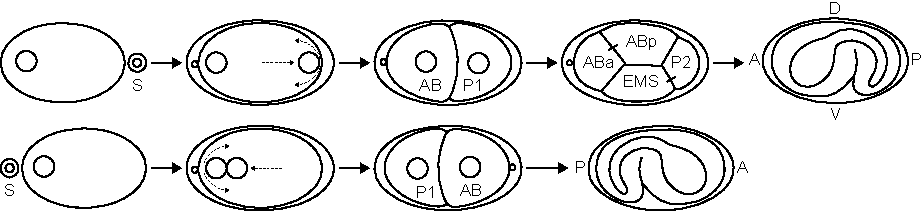
\includegraphics[width=0.9\textwidth]{Introduction/FigureBodyAxesGeometry/celegans.pdf}
    \caption{\acs{ap} axis in \acs{ce} establishes along the long axis of the ellipsoidal embryo, with posterior half determined by site of sperm entry \citep{goldstein1996specification}. S denotes the sperm at fertilization; AB, P1, ABa, ABp, P2, EMS are names of subsequent blastomeres in embryogenesis (see \autoref{subsec:EarlyEmbryoCelegans} and \cite{strome1989generation}). Top: Sperm enters on the right, away from the female pronucleus -- leading to an embryo with anterior on the left and posterior on the right. Bottom: Sperm enters on the left -- leading to an embryo with anterior on the right and posterior on the left. DV indicates dorso-ventral axis. Adapted from \cite{goldstein1997axis}}
    \label{subfig:compareBodyAxesEmbryoGeometry-apAxisCelegans}
\end{subfigure}
\hfill
\begin{subfigure}{\textwidth}
    \centering
    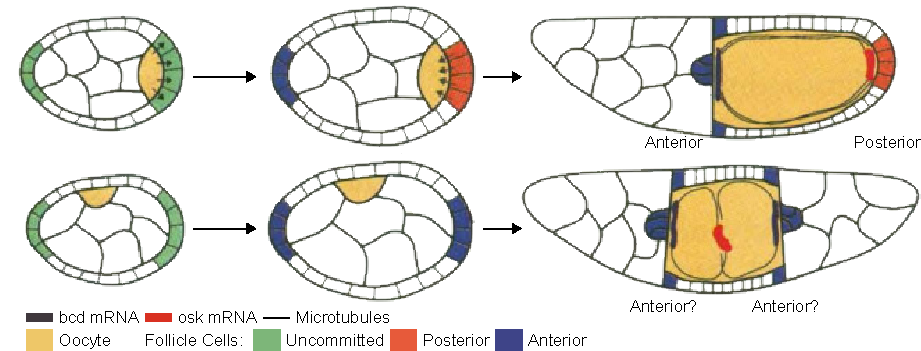
\includegraphics[width=0.9\textwidth]{Introduction/FigureBodyAxesGeometry/drosophila.pdf}
    \caption{\acs{ap} axis in \textit{Drosophila} is established along the long axis during oogenesis, with posterior half determined by location of oocyte within the germline cyst \citep{gonzalez1994role}. Top: in the usual case, the oocyte migrates towards the posterior of the cyst, specifying the posterior follicle cells that help determine the posterior end. Bottom: if this migration does not occur, no \acs{ap} axis is established. Adapted from \cite{gonzalez1994role}}
    \label{subfig:compareBodyAxesEmbryoGeometry-apAxisDrosophila}
\end{subfigure}
\hfill
\begin{subfigure}{\textwidth}
    \centering
    \includegraphics[width=0.9\textwidth]{Introduction/FigureBodyAxesGeometry/mouse.pdf}
    \caption{\acs{ap} axis in mouse is established during uterine implantation. Initial \acs{ap} axis forms along the long axis (Proximal-Distal) of the cylindrical embryo, indicated by the emergence of distal visceral endoderm (DVE) cells at E5.5. \acs{ap} axis reorients to the short axis as the DVE cells migrate to the lateral side, forming anterior visceral endoderm (AVE). Adapted from \cite{matsuo2017mechanical}}
    \label{subfig:compareBodyAxesEmbryoGeometry-apAxisMouse}
\end{subfigure}

\caption[Comparing orientation of \acs{ap} axis with geometry]{Comparing orientation of \acs{ap} axes with embryo geometry in different model organisms: \acs{ce}, \textit{Drosophila}, and mouse}
\label{fig:compareBodyAxesEmbryoGeometry}

\end{figure}

How does this orientation with respect to geometry achieved? Given that mechanical forces are involved in the establishment of body axes, could it be possible that the mechanical forces involved in body axes establishment play a role in achieving this relative orientation? Studies in the mouse embryo seem to suggest so \citep{vianello2019understanding,hiramatsu2013external,matsuo2017mechanical}, but how do mechanical forces enforce this relative orientation is not understood. In this thesis, we will study this problem in the context of \ac{ap} axis establishment in the \ac{ce} embryo - a nematode. We seek to understand the mechanism that ensures that the \ac{ap} axis of the \ac{ce} embryo always establishes along the long axis of the ellipsoidal embryo. 

In this chapter, we first introduce the general features of the cytoskeleton in eukaryotic cells. We will also describe the actomyosin cortex, an important higher-order structure of cytoskeletonal elements present in almost all eukaryotic cells. We then introduce the model organism used in this study: \ac{ce}. We describe the early development of the \ac{ce} embryo. Next, we describe the establishment of \ac{ap} axis in the one-cell stage \ac{ce} embryo. We also introduce the phenomenon of \ac{ap} axis alignment -- the active reorientation of the \ac{ap} axis such that it aligns with the geometric long axis of the ellipsoidal embryo. Finally, we provide an overview of the thesis, encapsulating our work on elucidating the mechanism of \ac{ap} axis alignment in \ac{ce} embryo.

\section{Cytoskeleton}\label{sec:Cytoskeleton}
As noted above, mechanics plays an important role in the establishment of body axes. Cells thus need to react to the mechanics of their surrounding, and modify their own mechanical properties in response to different stimuli. The structure that allows cells to actively modify their mechanical properties, and perform mechanical tasks, is the cytoskeleton \citep{chaffey2003alberts,bray2001cell,fletcher2010cell}. It is essential in many cellular processes: maintaining cell shape \citep{chaffey2003alberts,rivero1996role,herrmann2007intermediate}, driving locomotion \citep{fletcher2010cell}, and cell division \citep{chaffey2003alberts,gonczy2001spindle}. Its role is to provide the cell with a dynamic mechanical scaffolding, allowing the cell to act as a highly adaptive mechanical entity to achieve different tasks \citep{chaffey2003alberts,bray2001cell,fletcher2010cell}.

The cytoskeleton is commonly defined as a network of protein filaments that extend throughout the cytoplasm of eukaryotic cells, although analogous filaments have also been identified in prokaryotes \citep{erickson2007evolution}. This meshwork of filaments is complemented by motor proteins that exert force betwen the filaments, crosslinking proteins that tie these filaments in the meshwork and various associated proteins that modify and remodel the meshwork \citep{chaffey2003alberts,bray2001cell,fletcher2010cell}. In this section, we will introduce these elements that make the cytoskeleton in eukaryotic cells. We will also introduce the actomyosin cortex, a thin layer of cytoskeletonal elements present just below the cell membrane \citep{chaffey2003alberts,salbreux2012actin}, and the primary force-generating mechanical structure that this work focuses on.

\subsection{Main constituents of the cytoskeleton}\label{subsec:ComponentsCytoskeleton}
\subsubsection{Protein Filaments}\label{subsubsec:FilamentsCytoskeleton}
Protein filaments provide the backbone of the cytoskeleton. In eukaryotic cells, the cytoskeleton is composed of three principal types of protein filaments: actin filaments, intermediate filaments and microtubules. Monomeric protein subunits build each of these filaments. In contrast to usual polymers, these filaments are held together by non-covalent bonds, allowing fast assembly and disassembly \citep{chaffey2003alberts}. 

\paragraph{Actin filaments}
Actin filaments (or F-actin) are right-handed double helix composed of two protofilaments, each being a chain of actin monomers (or G-actin) \citep{pollard1986actin,pollard2000molecular} (see \autoref{subfig:cytoskeletonMainConsituents-actin}). Actin filaments are thin, with a typical diameter of around \SI{7}{\nano\meter} \citep{cooper2007cell}, and flexible, with a typical persistence length of \SI{17}{\micro\meter} \citep{ott1993measurement,gittes1993flexural}. The pitch of the helix formed by the protofilaments is typically around \SI{37}{\nano\meter}. Polymerisation of actin filaments is fueled by hydrolysis of \ac{atp} at the binding site on the monomers as they bind to the filament \citep{fujiwara2007polymerization}. Actin filaments are structurally polar, with a defined (+) or barbed end where new monomers preferentially bind, and a (-) or pointed end where monomers preferentially unbind \citep{pollard1986actin,pollard2000molecular,vavylonis2005actin}. Thus, actin filaments can undergo tread-milling, regulated by \ac{atp} \citep{wegner1982treadmilling}.

Actin filaments often gets organized into higher-order structure, such as the actomyosin cortex (which we describe below), to perform various functions such as migration \citep{pollard2003cellular}, cell division \citep{sanger1975changing} and control of cell shape \citep{clarke1977nonmuscle}. 

\paragraph{Microtubules}
Microtubules are rigid hollow rod-like polymers, formed by the polymerization of a dimer of two globular proteins, $\alpha$-tubulin and $\beta$-tubulin \citep{chaffey2003alberts,nogales1998structure} (see \autoref{subfig:cytoskeletonMainConsituents-microtubule}). These dimers polymerize to form linear protofilaments that associate laterally to form the microtubule \citep{chaffey2003alberts}. Slight offset between protofilaments generates a pseudo-helical structure \citep{hunyadi2007microtubule}. The typical \enquote{\num{13}-\num{3}} arrangement, composed of \num{13} protofilaments with \num{3} dimer offset between neighbouring pairs, has a diameter of approximately \SI{25}{\nano\meter}, and a persistence length of approx \SI{5}{\milli\meter} \citep{chalfie1979organization,chaffey2003alberts,gittes1993flexural,ledbetter1963microtubule} -- practically rigid in most cells, given their typical sizes. Similar to actin filaments, microtubules are also polar, with a fast growing (+) end and a slow growing (-) end \citep{howard2003dynamics}. Microtubules serve various functions such as providing mechanical support, facilitating cell migration and locomotion \citep{mikhailov1998relationship}, acting as pathways for intracellular transport \citep{chaffey2003alberts}, and centering of the mitotic spindle \citep{pearson2004dynamic,grill2003distribution,grill2005theory}.

\textit{Centrosome}: Microtubules usually are nucleated at, and extend outwards from, a \ac{mtoc}, to which the (-) ends are attached. In animal cells, the major \ac{mtoc} is the centrosome, typically present near the nucleus when the cell is not dividing. At mitosis (i.e. when the cell is dividing), the centrosome duplicates \citep{chaffey2003alberts}. In most animal cells, a centrosome consists of a pair of cylinders (centrioles) surrounded by a meshwork of pericentriolar material \citep{pimenta2020pericentriolar}. Complexes of $\gamma$-tubulin in the centrosome serve as the nucleation sites for microtubule assembly \citep{kellogg1994centrosome}. In many animals, centrosomes play an important role in the formation of the mitotic spindle, an array of microtubules and associated proteins responsible for proper segregation of genetic material in the daughter cells after division \citep{bettencourt2013q,chaffey2003alberts}.

\paragraph{Intermediate filaments}
Different cell types also produce other filaments, with a typical diameter of \SI{10}{\nano\meter}. They typically play a structural role and provide mechanical support \citep{chaffey2003alberts,herrmann2007intermediate}.

\subsubsection{Motor proteins}\label{subsubsec:MotorCytoskeleton}
Motor proteins convert the chemical energy released in \ac{atp} hydrolysis into mechanical work \citep{chaffey2003alberts,bray2001cell,kolomeisky2007molecular,howard2002mechanics}. Motor proteins are categorized into three super-families, distinguished by the type of filaments they bind to. \textit{Myosins} are motors associated with actin filaments, while \textit{kinesins} and \textit{dyenins} bind to microtubules instead \citep{chaffey2003alberts}. Molecular motors perform various functions \citep{chaffey2003alberts}, such as cargo transport \citep{vale2003molecular} and serving as force generators for contraction of large-scale structures \citep{howard2002mechanics,carlsson2006contractile}.

Generally, motor proteins share a common set of \enquote{mechanical parts}: a track on which the motor walks (typically the protein filaments), some fuel (typically \ac{atp}), a transducer and force generator that converts the chemical energy of the fuel into a \enquote{power stroke} to generate mechanical force and a lever that transmits that force to the track \citep{hwang2009mechanical}. We illustrate this using the example of a particular myosin - \acs{nmy2}, which is a major component of the actomyosin cortex. 

\paragraph{\acl{nmy2}}
\ac{nmy2} is a member of the myosin super-family of motor proteins, and therefore a molecular motor that acts on actin filaments (see \autoref{subfig:cytoskeletonMainConsituents-myosin}). It is a major contractile protein of non-muscle eukaryotic cells \citep{chaffey2003alberts,holmes2008myosin}. \ac{nmy2} forms a hexamer consisting of three pairs of polypeptides: two heavy chains, two regulatory light chains involved in regulation of \ac{nmy2} activity and two essential light chains which stabilize the heavy chain conformation \citep{holmes2008myosin,vicente2009non}. Each heavy chain has a motor domain on one end (N-terminus) that binds to actin filament and \ac{atp}, followed by a neck domain to which the regulatory light chains bind, and a coiled-coil domain on the other end (C-terminus) that facilitates dimerization of the heavy chain \citep{holmes2008myosin,vicente2009non,robert2019force}. \ac{nmy2} usually organizes into myosin minifilaments, consists of around \num{28} \ac{nmy2} units \citep{holmes2008myosin,vicente2009non}. 

How does the \ac{nmy2} motor generate force? When not bound to \ac{atp}, myosin has a strong affinity to actin filament. \ac{atp} binding leads to dissociation of the motor domain from the actin filaments, and \ac{atp} hydrolysis ensues. During this step, the neck domain bends, allowing the motor domain to sample sites on the actin filaments. As myosin binds again to the filament, the products of \ac{atp} hydrolysis are released, resulting in the force generating step (that is, the power stroke) that displaces the motor along the filament with \SI{5}{\nano\meter} displacement, and returns it back to the initial state \citep{de2004relating,sweeney2010structural,tyska2002myosin,robert2019force}. We refer the reader to \autoref{subfig:cytoskeletonMainConsituents-powerstroke} for a depiction of the power stroke of myosin. Thus, the motor domains act as the transducer and force generators, the neck domain as the lever, the actin filament as the track and \ac{atp} as fuel for the \ac{nmy2} motor \citep{robert2019force,hwang2009mechanical}. \ac{nmy2} is a non-processive motor (it only makes one step before it detaches from the track \citep{howard2002mechanics,hwang2009mechanical}) with a low duty cycle (fraction of time spent bound to actin filament \citep{howard2002mechanics,hwang2009mechanical}) \citep{kovacs2003functional,wang2003kinetic}. Minifilaments of \ac{nmy2} can slide actin filaments past each other, by creating force dipoles \citep{vicente2009non,niederman1975human,mahajan1996assembly}. \ac{nmy2} also serves as an actin crosslinker \citep{xu2001during,mizuno2007nonequilibrium,laevsky2003cross}.

\begin{figure}[p]

\centering
\begin{subfigure}{\textwidth}
    \centering
    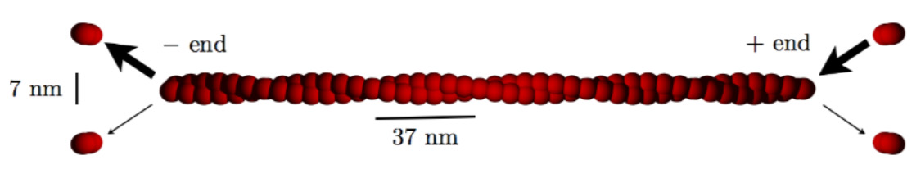
\includegraphics[width=0.9\textwidth]{Introduction/FigureCytoskeleton/actin.pdf}
    \caption{Sketch of an actin filament, red circles denote monomeric G-actin. Arrows indicate rate of chemical reaction at each end. Adapted from \cite{sebastian2012activeChiral}}
    \label{subfig:cytoskeletonMainConsituents-actin}
\end{subfigure}
\hfill
\begin{subfigure}{\textwidth}
    \centering
    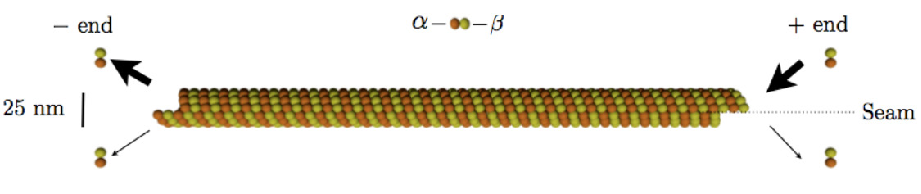
\includegraphics[width=0.9\textwidth]{Introduction/FigureCytoskeleton/microtubules.pdf}
    \caption{Sketch of a \enquote{13-3} microtubule, composed of $\alpha$ and $\beta$ tubules. Arrows indicate rate of chemical reaction at each end. Adapted from \cite{sebastian2012activeChiral}}
    \label{subfig:cytoskeletonMainConsituents-microtubule}
\end{subfigure}
\hfill
\begin{subfigure}{\textwidth}
    \centering
    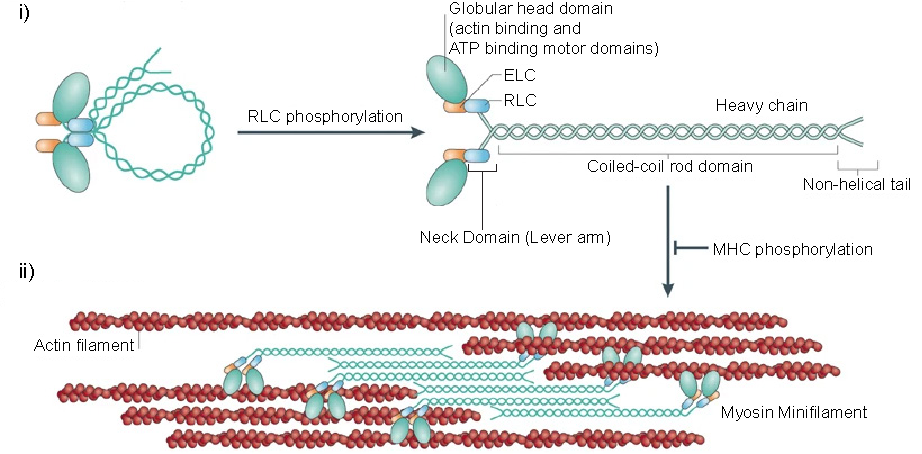
\includegraphics[width=0.9\textwidth]{Introduction/FigureCytoskeleton/myosin.pdf}
    \caption{Schematic of the forms of \acs{nmy2} motor protein. i) \acs{nmy2} converts from inactive state (left) to active state (right) via phosphorylation. Active state has three domains: the globular head containing the motor and actin binding domains, the neck domain or lever arm, and a long coiled-coil domain of heavy chains. ii) \acs{nmy2} can assemble into bipolar filaments -- myosin minifilaments -- and can slide antiparallel actin filaments past each other. Adapted from \cite{vicente2009non}}
    \label{subfig:cytoskeletonMainConsituents-myosin}
\end{subfigure}
\hfill
\begin{subfigure}{\textwidth}
    \centering
    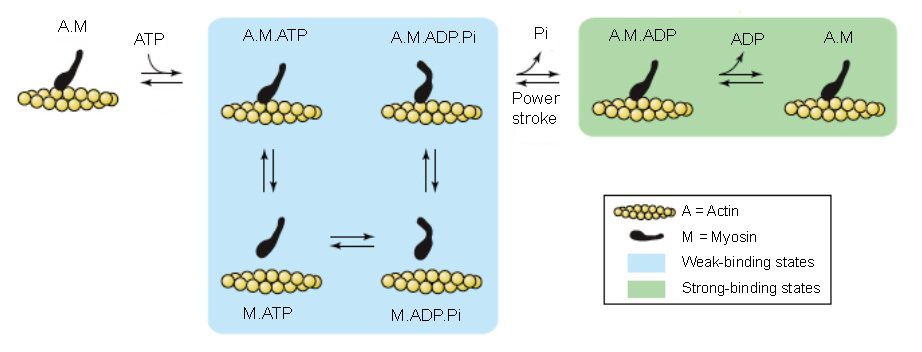
\includegraphics[width=0.85\textwidth]{Introduction/FigureCytoskeleton/powerstroke.pdf}
    \caption{Schematic of the power stroke of \acs{nmy2}. Refer to text for details on power stroke. Adapted from \cite{de2004relating}}
    \label{subfig:cytoskeletonMainConsituents-powerstroke}
\end{subfigure}

\caption[Main constituents of the cytoskeleton]{Main constituents of the cytoskeleton in eukaryotic cells}
\label{fig:cytoskeletonMainConsituents}

\end{figure}

\subsubsection{Associated proteins}\label{subsubsec:AssociatedProteinsCytoskeleton}
Most of the known cytoskeletal proteins are neither filamentenous nor motors. Instead, they modify and interact with the existing protein filaments and motors, to dynamically alter the mechanical properties of the cytoskeleton. We refer the reader to \cite{chaffey2003alberts,pollard1986actin} for a comprehensive overview of these proteins and their functions; here, we will briefly review some of the important functions these proteins fulfill.

\textit{Nucleators} help initiate the formation of protein filaments, by providing a nucleation point. \textit{Capping proteins} bind to the ends of filaments, blocking polymerisation at the end where they bind. These proteins thus can either stabilise or de-stabilise a protein filament, depending on where they bind. \textit{Severing proteins} cut filaments. \textit{Crosslinkers} and \textit{bundling proteins} organize protein filaments into structured networks, and modify them. \textit{Sequestering proteins} help with recycling unbound monomers, while \textit{Sidebinding proteins} act as molecular rulers. \textit{Linkers} link filaments of different kinds, allowing different filaments (such as the microtubules and actin filaments) to influence each other. \textit{Regulators} regulate the action of other proteins. Note that individual proteins can have multiple functions, and thus belong to multiple categories.

\subsection{Actomyosin cortex}\label{subsec:ActomyosinCortex}

\begin{figure}[h]
    \centering
    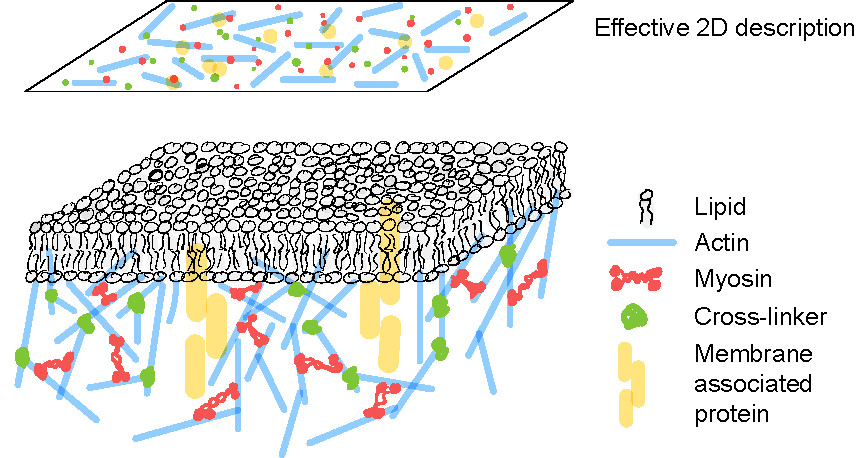
\includegraphics[width=\textwidth]{Introduction/FigureActomyosin/actomyosinSketch.pdf}
    \caption[Sketch of actomyosin cortex]{Sketch of the actomyosin cortex as a quasi-2D polymeric meshwork of actin filaments below the cell membrane (composed of lipids) and interspersed with myosin motors and other proteins. Top represents an effective 2D representation of the actomyosin cortex that could be obtained by averaging over the thickness of the cortex. Adapted from \cite{kumar2021actomyosin}}
    \label{fig:actomyosinCortexSketch}
\end{figure}

The actomyosin cortex, also called the cell cortex, is a thin (around few hundred nanometers \citep{clark2013monitoring}) polymeric meshwork of cross-linked actin filaments, interspersed with myosin motors and associated proteins, that lies just below the cell membrane of most eukaryotic cells \citep{bray1988cortical,chaffey2003alberts} (see \autoref{fig:actomyosinCortexSketch}). Analysis using cryo-electron tomography and atomic force microscopy revealed that actin filaments organize in both isotropic meshworks and actin bundles \citep{hartwig1991cytoskeleton,heuser1980filament,morone2006three,medalia2002macromolecular,pesen2005micromechanical}. 

The cortex is not, however, a static structure -- \ac{atp} hydrolysis fuels the polymerization and de-polymerization of actin filaments, activity of the associated proteins, and force generation by myosin motors. This external energy input and resultant active remodeling of the cortex drives it far from equilibrium, and makes it a very dynamic structure. This highly cross-linked and dynamic nature of the cortex makes it behave like a viscoelastic material \citep{kumar2021actomyosin,salbreux2012actin}, as confirmed by laser ablation experiments \citep{saha2016determining,mayer2010anisotropies}. In live cells, the active remodeling in the cortex occurs on timescales of around \SI{30}{\second} \citep{fritzsche2016actin}, and elastic stresses relax on comparable timescales \citep{saha2016determining}. As a consequence, the cortex can effectively be considered as a viscous fluid on longer timescales. Force generation by myosin motors confer the cortex with a tendency to actively contract \citep{carlsson2006contractile} -- the actomyosin cortex can thus be considered as active viscous fluid. In \autoref{ch:ActiveMatter}, we will discuss the behaviour of actomyosin cortex as an active fluid in the context of the \ac{ce} cortex during \ac{ap} axis establishment.

Actomyosin cortex helps the cell to adapt to changing environmental conditions by controlling cell mechanics. The cortex determines the stiffness of the cell surface, and opposes osmotic pressure \citep{stewart2011hydrostatic}. Global increase in contractility of the cortex facilitates the rounding of the cell before its division \citep{kunda2008moesin}. Local changes in cortex contractility can create gradients of cortical tension. Such changes can aid in cell migration, via retraction of the rear of the cell from the substrate \citep{vicente2009non}. Developmental processes at the tissue scale can also be directed by the cortex of the constituent cells \citep{rauzi2011cortical} -- such as dorsal closure in \textit{Drosophila} \citep{martin2010pulsation} and convergence extension in \textit{Xenopus} \citep{zhou2009actomyosin}. In \autoref{sec:ApAxisEstablishment}, we will discuss how the local changes in contractility in the one-cell stage \ac{ce} embryo drive flows in the cortex, and what role these cortical flows play in the \ac{ap} axis establishment of \ac{ce} \citep{mayer2010anisotropies}.

\section{\acs{ce} as a model organism}\label{sec:CelegansModel}

\begin{figure}[h]
    \centering
    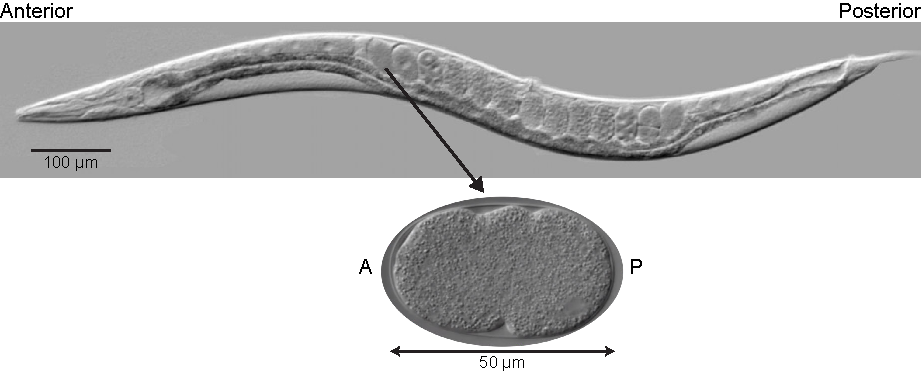
\includegraphics{Introduction/FigureWorm/worm.pdf}
    \caption[\acs{ce} worm and one-cell embryo]{Microscope picture of \acs{ce} worm (top) and one-cell stage embryo (bottom), by M. Leaver (used with permission). A and P mark the anterior and posterior of the developing embryo. Typical location of the one-cell embryo in the gonad of the worm, and its length (approx. \SI{50}{\micro\meter}) is marked}
    \label{fig:celegansWormModelOrganism}
\end{figure}

\ac{ce} was first considered as a potential model organism by Sydney Brenner over 50 years ago. After witnessing the importance of the T4 bacteriophages as the ideal 'model organisms' for research in molecular biology, he searched for a model organism to replicate the same successes in developmental biology and neuroscience \citep{wb1988nematode,brenner1974genetics,brenner2003nature}. He found his model organism of choice in the small nematode \ac{ce}, a self-fertilizing hermaphrodite with rare spontaneous males (less than \num{0.2}\% of worms \citep{haag2005evolution,corsi2015transparent}) \citep{brenner1974genetics}. Today, there are more than thousand research groups that use \ac{ce} as a model organism, due to the above ease of maintenance and the multitude of biological tools available for study and manipulation of \ac{ce} worms, in various fields such as neuroscience, development, ecology and cell biology \citep{corsi2015transparent}.

\ac{ce} is a free-living transparent nematode, typically found in temperate climate around the world. It feeds on bacteria, typically \ac{ecoli} on the surface of agarose plates when cultured in lab \citep{brenner1974genetics}. In lab conditions, \ac{ce} worms grow from initial larval stage (\SI{0.25}{\milli\meter} long) to final adult stage (\SI{1}{\milli\meter} long) in around \num{3} days at \SI{20}{\celsius}, although this time can vary with temperature and food available \citep{corsi2015transparent,brenner1974genetics,lee2009regulation}. It is a simple organism in both anatomy and genome. It has a fixed, genetically determined, number of cells at the adult stage, with adult hermaphrodite at 959 somatic cells and adult male at 1033 cells \citep{sulston1983embryonic,kimble1979postembryonic}. One of most prominent features of \ac{ce} is its invariant cell lineage: every worm follows the same pattern of cell divisions and results in the same number of cells, i.e. the developmental fate of every somatic cell is invariant. This has enabled tracing the fate of cell during development, giving rise to a complete map of cell lineage \citep{sulston1983embryonic,sulston1975dopaminergic,kimble1979postembryonic}. 

Hermaphrodites and males differ in their adult morphology, with males being a bit thinner and shorter, and possess a distinctive tail \citep{corsi2015transparent}. The primary method of reproduction in \ac{ce} is via self-fertilization: hermaphrodites produce both sperms and oocytes, which fertilize each other. A hermaphrodite typically lays about 300 eggs. Males can also fertilize the hermaphrodites, allowing for a form of sexual reproduction. The young worms hatch and subsequently go through four larval stages (L1-L4) before adulthood. These adults are fertile for about \num{3} days, and have an average lifespan of about \numrange{2}{3} weeks \citep{corsi2015transparent}. In harsh conditions, larval development can be paused -- these worms can survive several months in a special state called dauer arrest \citep{hu2007dauer}.

The above properties of \ac{ce} make it very convenient to use as a model organism for development \citep{corsi2015transparent,brenner1974genetics}. It is easy to maintain and grow in bulk due to the large number of progeny and rapid life cycle. Worms can be easily frozen for years and revived later when needed. Individual worms can be easily observed at the level of single cells under the microscope due to their transparency. Its small size allows complete anatomical description even at the electron microscope level. Self-fertilization means a single worm can generate an entire population of its clones, while the rare males, which can be maintained, enable transfer of genetic markers between populations. \ac{ce} is also the first multi-cellular organism with a completely sequenced genome, containing about 18000 predicted genes \citep{c1998genome}. Together with the simple feeding method of double stranded \ac{rnai} in \ac{ce} \citep{kamath2003genome}, all these properties of \ac{ce} make genetic perturbations in \ac{ce} worms a simple and efficient process. Using fluorescent proteins such as \ac{gfp} to tag the proteins in the embryo allows in-depth study of its development \citep{chalfie1994green,boulin2006reporter}.

\subsection{Early embryogenesis in \acs{ce}}\label{subsec:EarlyEmbryoCelegans}

\begin{figure}

\centering
\begin{subfigure}{\textwidth}
    \centering
    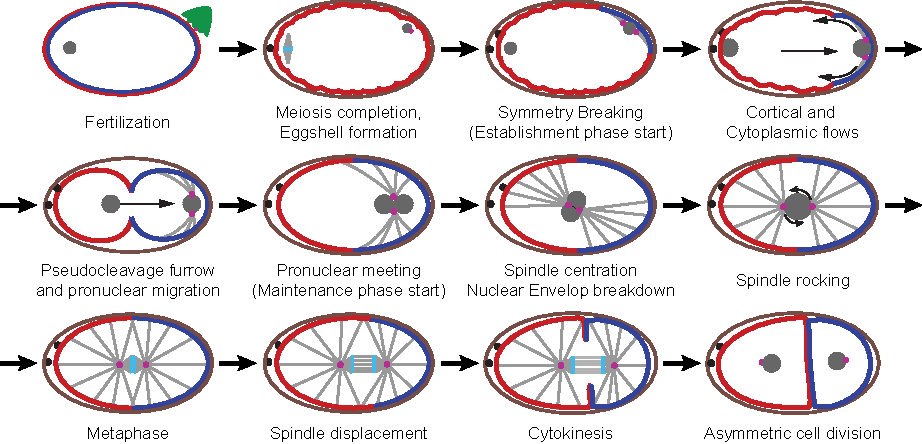
\includegraphics[width=\textwidth]{Introduction/FigureEarlyEmbryogenesis/firstCellEvents.pdf}
    \caption{Chronological sequence of events in the one-cell stage embryo, from fertilization until the first cell division. See \autoref{subsec:EarlyEmbryoCelegans} and \autoref{subsec:mechanismApAxisEstablishment} for further details. Anterior is to the left, posterior to the right. Grey circles represent pronuclei and nuclei, black circle extruded polar bodies, purple circle centrosomes. Microtubules are denoted in light grey, arrows illustrate movement. Blue represents \acs{ppar}, red represents \acs{apar}. Adapted from \cite{mirjam2010mechanics}. Also see \cite{schneider2003cell}.}
    \label{subfig:embryogenesisCelegans-onecell}
\end{subfigure}
\hfill
\begin{subfigure}{\textwidth}
    \centering
    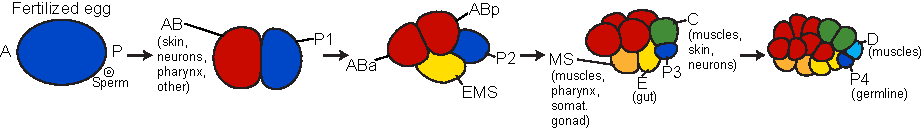
\includegraphics[width=\textwidth]{Introduction/FigureEarlyEmbryogenesis/fullEmbryogenesis.pdf}
    \caption{Sketch depicting early embryogenesis in \acs{ce} embryo. The one-cell stage embryo, after fertilization, undergoes an asymmetric division, forming the larger, anterior AB cell and smaller, posterior P1 cell. AB gives rise to somatic cells only. P1 divides further, generating somatic blastomeres EMS (which divides into E and MS), C and D, and the germline progenitor P4. Tissues that the blastomeres give rise to are indicated next to them. Adapted from \cite{mirjam2010mechanics}. Also see \cite{strome1989generation}.}
    \label{subfig:embryogenesisCelegans-full}
\end{subfigure}

\caption[Early embryogenesis in \acs{ce}]{Early embryogenesis in \acs{ce} embryo}
\label{fig:embryogenesisCelegans}

\end{figure}

\ac{ce} embryogenesis begins when a mature oocyte, arrested in meiosis I, is fertilized by a sperm \citep{rose2014polarity,begasse2011} -- see \autoref{subfig:embryogenesisCelegans-onecell}. As we will discuss later on, the site of sperm entry defines the future posterior end of the embryo \citep{goldstein1996specification} (also, see \autoref{subfig:compareBodyAxesEmbryoGeometry-apAxisCelegans}). Prior to fertilization, the oocyte is fairly symmetric \citep{cuenca2003polarization,cowan2004asymmetric,schonegg2006cdc}. Thus, sperm entry represents the first event in which symmetry is broken in the oocyte. At fertilization, the sperm donates its genetic material -- the male pronucleus -- to the embryo, along with centrosomes \citep{o2000spd,wallenfang2000polarization,cowan2004centrosomes}. After fertilization, meiosis is completed with the extrusion of two polar bodies, usually located at the anterior end. A rigid ovoid-shaped chitin eggshell is secreted by the newly formed embryo after fertilization -- which provides the embryo with its ellipsoidal shape \citep{johnston2012eggshell}.

Events in the one-cell stage of the \ac{ce} embryo -- called the P0 stage -- can be divided into two phases: establishment phase and maintenance phase \citep{cuenca2003polarization}. Establishment phase is initiated by the centrosomes near the male pronucleus. These centrosomes organize microtubule asters, which lead to triggering the establishment of the \ac{ap} axis (discussed below). In the establishment phase, large-scale flows in the actomyosin cortex (directed away from the male pronucleus) and cytoplasm (directed towards the male pronucleus) are observed, which gives the establishment phase its other name -- flow phase. Towards the end of establishment phase, the female pronucleus migrates towards and meets with the male pronucleus, concomitant with a characteristic constriction at the mid of the embryo -- called the pseudocleavage furrow \citep{cuenca2003polarization,nigon1960architecture,reymann2016cortical}. This migration is powered by the microtubules connecting the two pronuclei late in the establishment phase \citep{niwayama2011hydrodynamic}. Pronuclear meeting indicates the end of establishment phase and start of the maintenance phase.

In the maintenance phase, the \ac{ap} axis orientation is maintained -- no flows in the actomyosin cortex or cytoplasm are observed. P granules, which play a role in determining germline fate, localize towards the posterior end, as dictated by the established \ac{ap} axis \citep{gonczy2008mechanisms,hoege2013principles}. The mitotic spindle is set up in the center of the embryo, but elongates towards the posterior end following pronucleus envelope breakdown \citep{grill2003distribution}. The spindle is observed to rock, i.e. oscillate \citep{grill2005theory}. Towards the end of maintenance phase, the P0 cell divides asymmetrically (due to the eccentric location of the mitotic spindle). This results in a large cell towards the anterior and a smaller cell at the posterior, termed AB and P1 respectively. 

These cells divide further as the embryo develops, as depicted in \autoref{subfig:embryogenesisCelegans-full}. The established AP axis is however retained by the distribution of P granules as the embryo develops, as the P granules segregate into the germline precursor cells: P1, P2, P3, P4 \citep{rose2014polarity,strome1989generation}. The P4 cell is the primodial germ cell -- all sperms and oocytes generated in the new worm originate from this P4 cell \citep{rose2014polarity,kimble2005germline}.

\section{\acs{ap} axis establishment in \acs{ce}}\label{sec:ApAxisEstablishment}
In this section, we will discuss in detail the mechanism of \ac{ap} axis establishment in \ac{ce}. As noted above, the \ac{ap} axis is established during the establishment phase at the one-cell stage during \ac{ce} embryogenesis \citep{rose2014polarity}. \ac{ap} axis is established via a cell polarization event mediated by \acs{par} polarity proteins \citep{motegi2013network,hoege2013principles,lang2017proteins}. In this section, we will first discuss the \acs{par} polarity system -- a conserved system of proteins involved in cell polarization in many eukaryotic cells \citep{hoege2013principles}. Next, we will discuss the \ac{ap} axis establishment process, detailing the role of the actomyosin cortex and the centrosomal trigger from the male pronucleus. Finally, we will introduce the phenomenon this work is mainly concerned with: \ac{ap} axis alignment. We will also discuss the proposed mechanisms for \ac{ap} axis alignment.

\subsection{\acs{par} polarity system}\label{subsec:ParPolarity}
\ac{par} proteins are a conserved set of proteins in eukaryotes, functioning to control asymmetric cell division and partitioning of components in many cell types \citep{goldstein2007proteins,knoblich2001asymmetric}, and crucial in cell polarity establishment \citep{goldstein2007proteins}. \ac{par} proteins were first identified in the \ac{ce} embryos, as a result of genetic mutations that cause symmetric division of the one-cell embryo \citep{guo1995par1,kemphues1988identification}. 

As noted above, \ac{par} proteins help establish the \ac{ap} axis in \ac{ce} via polarization of the one-cell stage embryo. \ac{par} proteins can be classified into three groups based on their localization in this polarized embryo: PAR-4 and PAR-5 remain uniformly distributed on the cortex, PAR-1, PAR-2, LGL-1 (\ac{ppar}) localize to the posterior half of the cortex and PAR-3, PAR-6, PKC-3 (\ac{apar}) localize to the anterior half of the cortex \citep{motegi2013network}. Importantly, this localization is specific to the cortex (but not absolute) - \ac{par} proteins are uniformly distributed in the cytoplasm \citep{motegi2013network,hoege2013principles}. 

Experiments using Fluorescent recovery after photo-bleaching and fluorescent correlation spectroscopy have revealed that \ac{par} proteins can exchange between the cortex and the cytoplasm, and also diffuse laterally on the cortex \citep{hoege2013principles,goehring2011proteins,schubert2000mex,petravsek2008characterization}. Extensive mixing between the \ac{apar} and \ac{ppar} on the cortex is prevented by the mutual inhibition between the two groups: \ac{apar} inhibit the binding of \ac{ppar} to the cortex occupied by \ac{apar}, and vice versa \citep{hoege2013principles,motegi2013network}. The behaviour of \ac{par} proteins on the cortex can be modelled as a reaction-diffusion system, with characteristics similar to those observed \emph{in vivo} \citep{hoege2013principles}. Importantly, \ac{par} proteins can interact with the actomyosin cortex -- \ac{apar} can reduce the dissociation rate of \ac{nmy2} from the cortex \citep{gross2019guiding}, while flows in the cortex can advect the \ac{par} proteins \citep{goehring2011advectionpolarization}. 

\subsection{Mechanism of \acs{ap} axis establishment}\label{subsec:mechanismApAxisEstablishment}

\begin{figure}

\centering
\begin{subfigure}{\textwidth}
    \centering
    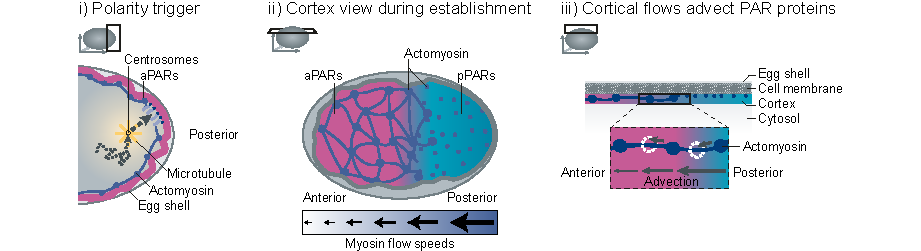
\includegraphics[width=\textwidth]{Introduction/FigureApAxisEstablishment/ApAxisEstablishmentEvents.pdf}
    \caption{Schematics depicting the major events that occur in \acs{ap} axis establishment in one-cell \acs{ce} embryo. i) Polarity trigger is provided by the centrosome towards the future posterior end of the embryo, via microtubules and other diffusive components \citep{hoege2013principles}. This trigger displaces the \acs{apar} and down-regulate the actomyosin cortex near the trigger \citep{hoege2013principles,gross2019guiding}. ii) View onto the cell Cortex during \acs{ap} axis establishment. Actomyosin cortex is less cross-linked and less dense in the posterior domain (indicated by \acs{ppar}) compared to anterior domain (indicated by \acs{apar}). The cortex also shows anisotropic tension \citep{mayer2010anisotropies}, with cortical flow directed towards the anterior. Flow speeds are larger in the posterior compared to anterior. iii) Cross-section of the cell cortex. Cortical flows passively transport the \acs{par} proteins by advection \citep{goehring2011advectionpolarization}. Adapted from \cite{hoege2013principles}} 
    \label{subfig:apAxisEstablishmentMechanism-schematics}
\end{subfigure}
\hfill
\begin{subfigure}{\textwidth}
    \centering
    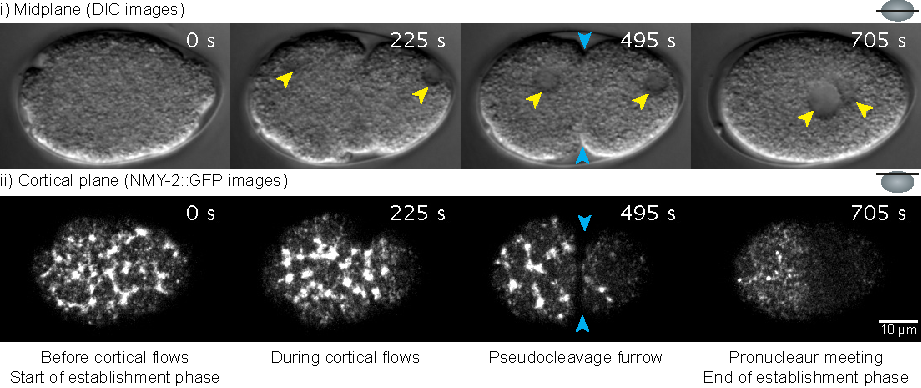
\includegraphics[width=\textwidth]{Introduction/FigureApAxisEstablishment/ApAxisEstablishmentCortexMicrograph.pdf}
    \caption{Cortical activity during \acs{ap} axis establishment. Top: DIC images taken in the midplane of the embryo. Bottom: \acs{nmy2}::\acs{gfp} images taken at the surface of the embryo; that is, in the cortical plane. Anterior is to the left, posterior to the right. $T=$ \SI{0}{\second} indicates start of establishment phase, with myosin forming foci-like structures uniformly in the cortex. After polarization is triggered near the male pronucleus, anterior-directed cortical flows cause the cortex to retrace from the posterior end (ex: $T=$ \SI{225}{\second}). The cortex completely retracts by the time the pseudocleavage furrow forms ($T=$ \SI{495}{\second}), and the two domains have formed. Establishment phase ends at pronuclear meeting ($T=$ \SI{705}{\second}), with myosin foci disappearing from the cortex. Yellow arrows indicate pronuclei (female on the left, male on the right) and blue arrows represent the ingression formed by the pseudocleavage furrow. Scale: \SI{10}{\micro\meter}. Adapted from \cite{sundar2012regulation}}
    \label{subfig:apAxisEstablishmentMechanism-micrograph}
\end{subfigure}

\caption[\acs{ap} axis establishment in \acs{ce}]{Mechanism of \acs{ap} axis establishment in one-cell stage \acs{ce} embryo}
\label{fig:apAxisEstablishmentMechanism}

\end{figure}

\ac{ap} axis establishment starts around \SI{30}{\minute} after fertilization, by the polarity trigger provided by the centrosomes associated with the male pronucleus \citep{o2000spd,wallenfang2000polarization,cowan2004centrosomes,de2020mitochondria}. Before the polarization trigger, the \ac{par} polarity network is primed \citep{zhao2019aurora,reich2019regulated,kapoor2019centrosome,klinkert2019aurora}, resulting in an initially unpolarized one-cell embryo with \ac{apar} uniformly enriched on the cortex \citep{cuenca2003polarization,cowan2004asymmetric,schonegg2006cdc}. 

As the male pronucleus approaches the cortex, the associated centrosome provides the polarity trigger to break this symmetric distribution and initiate \ac{ap} axis establishment \citep{wallenfang2000polarization,hoege2013principles,bienkowska2012centrosomes} -- see \autoref{subfig:apAxisEstablishmentMechanism-schematics}. This polarity trigger loads the \ac{ppar} onto the cortex near the centrosome, and thus near the male pronucleus \citep{wallenfang2000polarization,cowan2004centrosomes,gross2019guiding}. This nascent domain of \ac{ppar}, or the posterior domain, is protected from mutual inhibition from \ac{apar} by microtubules from the centrosome \citep{motegi2011microtubules}. Additionally, the polarity trigger inhibits actomyosin contractility near the male pronucleus by local down-regulation of \ac{nmy2} \citep{motegi2006sequential}. This generates an unequal distribution of myosin motors within the cortex, leading to active stresses in the cortex, and generating flows in the actomyosin cortex towards the future anterior end of the embryo and pointing away from the male pronucleus \citep{munro2004cortical,mayer2010anisotropies}. Cortical flows transport the \ac{par} proteins towards the anterior end via advection -- expanding the posterior domain \citep{goehring2011advectionpolarization}. Difference in the \ac{nmy2} dissociation rates between the posterior and anterior domains \citep{gross2019guiding} further drives the unequal distribution of myosin motors on the cortex, and thus promotes cortical flows. Modification of the actomyosin cortex, and thus cortical flows, can be observed in \ac{nmy2}::\ac{gfp} labelled movies of the \ac{ce} embryo, see \autoref{subfig:apAxisEstablishmentMechanism-micrograph}.

Additional to \ac{par} protein transport, cortical flows also generate cytoplasmic flows due to the drag between the cortex and the cytoplasm; with cytoplasmic flows being directed towards the male pronucleus due to the incompressible nature of the cytoplasm and embryo geometry \citep{niwayama2011hydrodynamic}. Thus, the male pronucleus is pushed into the cortex -- ensuring robust polarization of the embryo \citep{gubieda2020going}. 

Polarization of the embryo thus proceeds via a self-organized mechanochemical feedback loop between the \ac{par} polarity system and cortical flows guided by the polarity trigger from the centrosome \citep{gross2019guiding,bois2011pattern,gross2017active}. \ac{par} proteins control the flows in the cortex \citep{gross2019guiding} and cortical flows control the size of the \ac{par} domains \citep{munro2004cortical,goehring2011advectionpolarization}. Altogether, this process continues until the one-cell embryo is transformed from an initially unpolarized state to a polarized state. The polarization thus set up at the end of establishment phase establishes the \ac{ap} axis -- with the eventual anterior and posterior domains denoting the anterior and posterior end of the embryo. 

Converting this polarization into the \ac{ap} axis is accomplished by processes downstream of the \ac{par} proteins. \ac{par} domains on the cortex induce a cytoplasmic gradient of MEX-5 \citep{schubert2000mex}, which drives the segregation of P granules and various other \enquote{determinants}  towards the posterior end \citep{hoege2013principles}. Differential contractility of the actomyosin cortex in the posterior and anterior domains also sets up the stage for the asymmetric division of the one-cell embryo \citep{grill2003distribution}. Together, these processes ensure that the \ac{ap} axis established at the one-cell stage is realized as the embryo develops.

Note that in the following sections and chapters, unless specifically mentioned, we will always treat the centrosome as attached to the male pronucleus, and thus attribute the actions of the centrosome to the male pronucleus as a shorthand.

\subsection{\acs{ap} axis alignment}\label{subsec:ApAxisAlignment}

\begin{figure}

\centering
\begin{subfigure}{\textwidth}
    \centering
    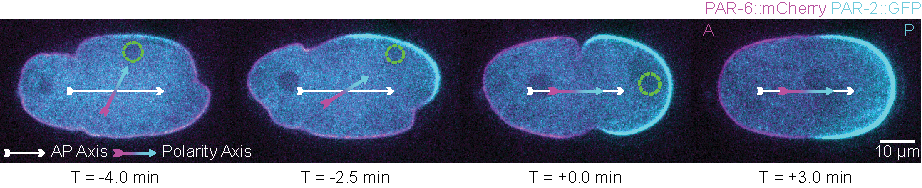
\includegraphics[width=\textwidth]{Introduction/FigureApAxisAlignment/micrograph.pdf}
    \caption{\acs{ap} axis alignment in \acs{ce} embryo, labelled with PAR-2::GFP, PAR-6::mCherry. In the untypical case where the \acs{ap} axis establishment is triggered away from the long axis of the embryo, the \acs{ap} axis -- defined as the orientation of the \acs{par} domains -- reorients towards the long axis of the ellipsoidal embryo. In this micrograph, PAR-2::GFP (in cyan) denotes the posterior domain (\acs{ppar}), and PAR-6::mCherry (in magenta) denotes the anterior domain (\acs{apar}). $T = $ \SI{0}{\minute} denotes the timepoint when the domains are fully established, and the male pronucleus moves away from the cortex. Green dashed circle denotes the male pronucleus. Instantaneous \acs{ap} axis (polarity axis) is denoted by arrow colored cyan to magenta, long axis of embryo is denoted by white arrow. Anterior is to the left, posterior to the right. The timepoints are depicting, in order, the start of establishment phase ($T = $ \SI{-4.0}{\minute}), an intermediate snapshot during cortical flows ($T = $ \SI{-2.5}{\minute}), formation of pseudocleavage furrow ($T = $ \SI{0.0}{\minute}), and pronuclear meeting ($T = $ \SI{3.0}{\minute}). Note the movement of the posterior \acs{par} domain along with the male pronucleus towards the right tip of the embryo -- such that the \acs{ap} axis aligns with the long axis. Images taken by P. Gross (used with permission)} 
    \label{subfig:apAxisAlignment-micrograph}
\end{subfigure}
\hfill
\begin{subfigure}{\textwidth}
    \centering
    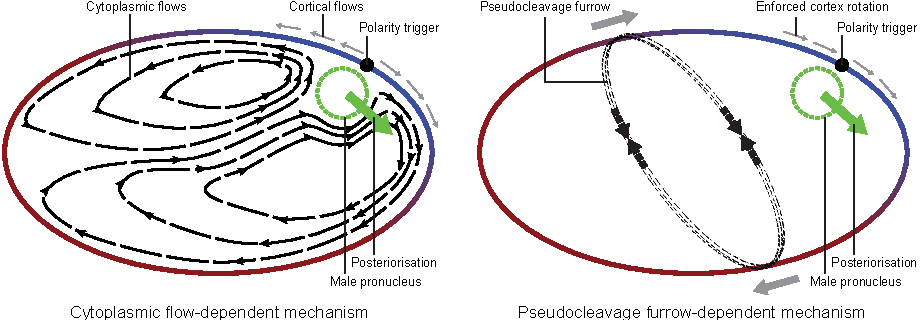
\includegraphics[width=\textwidth]{Introduction/FigureApAxisAlignment/mechanisms.pdf}
    \caption{Possible mechanisms for \acs{ap} axis alignment, driven by cortical flows. Cortical flows can drive flows in the cytoplasm (left) \citep{niwayama2011hydrodynamic} and lead to the formation of a contractile ring of actin around the embryo -- called the pseudocleavage furrow (right) \citep{reymann2016cortical}. Cytoplasmic flow-dependent mechanism (left): In the untypical case where the male pronucleus (green dashed circle) is not on the long axis of the embryo, the polarity trigger (black circle) generates cortical flows (grey arrows) asymmetrically. These leads to asymmetric cytoplasmic flows (black dashed), which can then advect the male pronucleus towards the closest tip (posteriorisation denoted by green block arrow). Pseudocleavage furrow-dependent mechanism (right): In the untypical case where the male pronucleus is not on the long axis of the embryo, the pseudocleavage furrow is generated not perpendicular to the long axis of the embryo. As this contractile ring (black dashed arrows denote contraction) rotates to attain a configuration with minimal length (denoted by grey block arrows), it forces the rotation of the cortex (denoted by grey thin arrows). This forces the male pronucleus towards the closest tip.}
    \label{subfig:apAxisAlignment-mechanisms}
\end{subfigure}

\caption[\acs{ap} axis alignment in \acs{ce}]{\acs{ap} axis aligns to the long axis in one-cell stage \acs{ce} embryo. Possible mechanisms of \acs{ap} axis alignment.}
\label{fig:apAxisAlignment}

\end{figure}

In our description of \ac{ap} axis establishment, we have so far neglected to mention the relation between the orientation of the \ac{ap} axis and the ellipsoidal-like geometry of the embryo. The ellipsoidal-like shape is imposed on the embryo by the eggshell surrounding it, which it secretes shortly after fertilization \citep{johnston2012eggshell}. The embryo has one long axis about \SI{50}{\micro\meter} in length, and two short axes about \SI{30}{\micro\meter} in length \citep{begasse2011,riddle1997celegans}. As we mentioned previously, the \ac{ap} axis in \ac{ce} always forms along the long axis of the ellipsoidal embryo \citep{goldstein1996specification}. How then are the AP axis and the geometric long axis aligned?

In the typical case, the sperm enters the embryo near long axis of the embryo. Thus, in the typical case, the male pronucleus and the centrosome are located near to the long axis -- ensuring that the \ac{ap} axis already establishes along the long axis. However, as described in \cite{goldstein1996specification}, the \ac{ap} axis will always form along the long axis -- \textbf{even if the male pronucleus is initially away from the long axis}. In this untypical case, which occurs due to lateral sperm entry (sperm entry away from the long axis), the \ac{ap} axis actively re-orient to align with the long axis. As shown in \autoref{subfig:apAxisAlignment-micrograph}, this is observed as the movement of \ac{par} domains to align correctly with the long axis, along with the migration of the male pronucleus with the posterior domain and towards the closest tip \citep{goldstein1996specification} -- we call this migration of the male pronucleus as posteriorisation. The mechanism(s) that drive(s) the alignment of \ac{ap} axis with the long axis is not currently understood.

Multiple mechanisms have been proposed in the past to explain \ac{ap} axis alignment. Observing that the cytoplasmic flows in the embryo are directed by the male pronucleus, \cite{goldstein1996specification} suggested that these cytoplasmic flows could drive the posteriorization. It was proposed that these flows could push onto the male pronucleus \citep{kimuraCytoplasmicFlows}, and owning to the geometry of the embryo in which the flows operate, push the male pronucleus towards the closest tip in the untypical case \citep{goldstein1996specification} -- see \autoref{subfig:apAxisAlignment-mechanisms}. Experiments with artificially generated cytoplasmic flows in maintenance phase indicate that cytoplasmic flows can influence the orientation of the \ac{ap} axis \citep{mittasch2018non}. Thus, in this mechanism, cytoplasmic flows act as a geometry-sensor. We refer to this proposed mechanism of \ac{ap} axis alignment as cytoplasmic flow-dependent mechanism. 

In this work, we propose another mechanism might also be at play. In addition to cytoplasmic flows, cortical flows also lead to the formation of the pseudocleavage furrow -- a contractile ring-like structure that forms at the boundary between the two PAR domains late in the establishment phase \citep{nigon1960architecture,reymann2016cortical}. Previous studies have found the pseudocleavage furrow to be not essential for \ac{ap} axis establishment \citep{rose1995pseudocleavage}, but indicate that it may play a role in the dynamics of \ac{ap} axis establishment \citep{aras2018importance}. We propose that the pseudocleavage furrow may play a role in \ac{ap} axis alignment. In the untypical case, the pseudocleavage furrow is not perpendicular to the long axis of the embryo. Akin to an elastic rubber-band on an ellipsoid, the pseudocleavage furrow could rotate to minimize its circumference and position itself perpendicular to the long axis, forcing the cortex to reposition such that the \ac{ap} axis aligns with the long axis  -- see \autoref{subfig:apAxisAlignment-mechanisms}. We refer to this mechanism as the pseudocleavage furrow-dependent mechanism. 

Other mechanisms proposed are concerned with the distribution of \ac{par} proteins, instead of the mechanics-based mechanisms considered above. \cite{gessele2018protein} proposes that the reaction-diffusion system constituted by the \ac{par} proteins on the ellipsoidal surface of the embryo is sufficient to attain the alignment of \ac{ap} axis with the long axis. However, this mechanism explicitly is considered in the absence of any activity of the actomyosin cortex -- and therefore explains any correction of the \ac{ap} axis during the later maintenance phase, not the alignment in the establishment phase. In fact, previous studies indicate that \ac{ap} axis alignment cannot occur during the establishment phase in the absence of any cortical activity \citep{zonies2010symmetry,motegi2011microtubules,tse2012nop1}. Additionally, \citep{klinkert2019aurora} has indicated that binding and unbinding of \ac{par} proteins to the cortex could be curvature sensitive -- which could also play a role in the geometry sensing required for \ac{ap} axis alignment.

\section{Overview}\label{sec:ApAxisOverview}
The aim of this work is to elucidate the mechanism that drives \ac{ap} axis alignment in the one-cell stage \ac{ce} embryo. Specifically, we will consider an active fluid description of the actomyosin cortex which can incorporate both the cytoplasmic flow-dependent and pseudocleavage furrow-dependent mechanisms. Using this description in conjugation with experiments that disable the pseudocleavage furrow, we will show that the pseudocleavage furrow-dependent mechanism is the predominant mechanism driving \ac{ap} axis alignment in \ac{ce}, with cytoplasmic flow-dependent mechanism a minor contributor. Further, we will explore the geometric dependence of \ac{ap} axis alignment. We will show that experimentally modifying the embryo geometry influences the \ac{ap} axis alignment process in a manner consistent with both our theoretical description of the cortex and a simplified model of the pseudocleavage furrow-dependent mechanism. 

The structure of the thesis is as follows. In \autoref{ch:ActiveMatter}, we will introduce the generic theory of active fluids, following \cite{julicher2018hydrodynamic,de2013non}. We will then discuss two models of the actomyosin cortex considered before in \cite{gross2019guiding} and \cite{reymann2016cortical}, and describe a combined description that incorporates both the cytoplasmic flow-dependent and pseudocleavage furrow-dependent mechanisms. In \autoref{ch:Exp}, we describe the experimental methods of our work. We detail how movies of embryos undergoing \ac{ap} axis alignment were obtained, how these movies were analysed to quantify posteriorization of the male pronucleus and cortical flows, and how genetic perturbations were made in \ac{ce} embryos. In \autoref{ch:Results}, we use the tools introduced in \autoref{ch:Exp} to test various hypotheses experimentally and compare their results to simulation results from the model developed in \autoref{ch:ActiveMatter}, in order to elucidate the mechanism of \ac{ap} axis alignment. Finally, in \autoref{ch:Summary}, we summarize our results from this work and discuss them in context of results from previous studies. 

\chapter{A theoretical model for \acs{ap} axis alignment}\label{ch:ActiveMatter}
In this chapter, the theoretical model for \ac{ap} axis alignment is described. The chapter is divided into three sections. The first section reviews the model of \ac{ap} axis establishment described in \cite{gross2019guiding}, which utilizes a reaction-diffusion-advection system to describe the distribution of \ac{par} proteins and \ac{nmy2}. The second section reviews the model of the formation of pseudocleavage furrow via compressive alignment of actin filaments due to flows in the actomyosin cortex, as described in \cite{reymann2016cortical}. The third section describes the theoretical model of \ac{ap} axis alignment used in this thesis, by combining the two models discussed in the sections before. It also describes the details of the numerical simulations of the theoretical model, and how the parameters of the model were calibrated using experimental data. The theoretical model was developed in collaboration with M. Nestler and A. Voigt, with numerical simulations and calibration done by M. Nestler -- further details on the model are described in \cite{axisConvergence}.

\section{A model of \acs{ap} axis establishment in \acs{ce}}\label{sec:apAxisEstablishModelPG}
As discussed in \autoref{sec:ApAxisEstablishment}, the centrosomes associated with the male pronucleus guide the establishment of \ac{ap} axis. In \cite{gross2019guiding}, the authors propose a model to investigate the centrosome-guided \ac{ap} axis establishment. In particular, the following components are included in the model proposed in \cite{gross2019guiding}:
\begin{itemize}
    \item Mutual antagonism between \ac{apar} and \ac{ppar} \citep{hoege2013principles} is captured via a mass-conserved Turing-like system \citep{goehring2011advectionpolarization,lee2015self,halatek2018rethinking}
    \item Mechanochemical feedback between the \ac{par} polarity system and actomyosin cortex is captured via coupling this Turing-like system to an active isotropic fluid description of the cortex \citep{mayer2010anisotropies,bois2011pattern}
    \item Spatiotemporal cues provided by the centrosomes associated with the male pronucleus (for loading of \ac{ppar} and depletion of myosin on the cortex) are captured as two distinct guiding cues -- \ac{ppar} stabilization cue and actomyosin cue, with the latter having two components.
\end{itemize}
This section describes this model of \ac{ap} axis establishment introduced in \cite{gross2019guiding}. This model assumes that the male pronucleus is always present at the posterior end, and thus assumes rotational symmetry around the long axis of the embryo. This simplifies the model to a 1-dimensional model of length $L$ with periodic boundary conditions, along the boundary of the cross-section at the midplane of the embryo \citep{gross2019guiding}. The posterior end is considered to be at the center of the domain $x \in [-\frac{L}{2},\frac{L}{2}]$ -- that is, at $x = 0$ (see \autoref{fig:apAxisEstablishModelPG}). Note that the curvature of the embryo boundary is neglected in this model.

\begin{figure}
\centering
\begin{subfigure}{\textwidth}
    \centering
    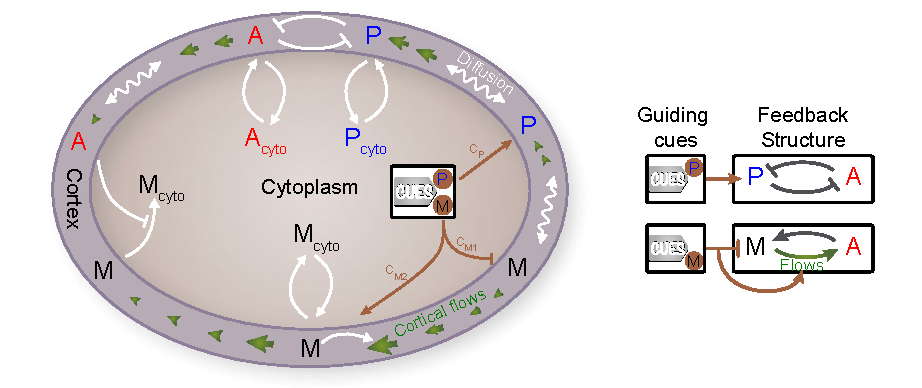
\includegraphics[width=\textwidth]{ActiveMatterModel/FigureModelPG/modelPG.pdf}
    \caption{Schematic depicting the Turing-like system for \ac{apar} $A$, \ac{ppar} $P$ and myosin $M$. These proteins are either located in the cytoplasm (denoted using the $cyto$ subscript) or at the cortex, where they are subjected to lateral diffusion and advective transport by cortical flows. The following reactions are considered: spontaneous association with and dissociation from the cortex, mutual antagonism between \ac{apar} and \ac{ppar} when associated to the cortex, and \ac{apar} regulated dissociation of myosin from the cortex. Two guiding cues are provided by the centrosomes and steer the \ac{ap} axis establishment process: \ac{ppar} domain stabilisation cue (denoted by $c_P$) and actomyosin cue with two components -- one depleting myosin at the cortex (denoted by $c_{M1}$) and the other regulating contractility (denoted by $c_{M2}$. See \autoref{sec:apAxisEstablishModelPG} for details.}
    \label{subfig:apAxisEstablishModelPG-schematic}
\end{subfigure}
\hfill
\begin{subfigure}{\textwidth}
    \centering
    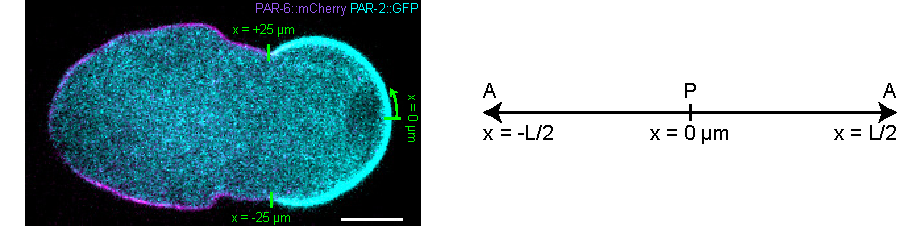
\includegraphics[width=\textwidth]{ActiveMatterModel/FigureModelPG/par2Par6SymmetricArclength.pdf}
    \caption{Left: Mid-plane section of the \acs{ce} embryo, labelled with PAR-2::\ac{gfp} (posterior domain, in cyan) and PAR-6::mCherry (anterior domain, in magenta). The model discussed in \autoref{sec:apAxisEstablishModelPG}, using the rotational symmetry around the long axis, is reduced to a 1-dimensional model along the boundary of this mid-plane section, endowned with the arclength variable $x$. $x$ is annotated in green -- $x = 0$ denotes the posterior pole. Scale bar: \SI{10}{\micro\meter}. Note that the positive and negative \enquote{arm} of the boundary is flipped compared to that in \cite{gross2019guiding} following the convention followed in this thesis. Right: Boundary of the cross-section at the midplane of the embryo reduced to a 1-dimensional line with periodic boundary conditions. $x = 0$ is at the posterior pole (denoted by P), and $x = \pm \flatfrac{L}{2}$ at the anterior (denoted by A).}
    \label{subfig:apAxisEstablishModelPG-arclengthMidplaneBoundary}
\end{subfigure}
\caption[Schematic representing the \acs{ap} axis establishment model in \cite{gross2019guiding}]{Schematic representing the 1-dimensional model of \acs{ap} axis establishment described in \cite{gross2019guiding}, and visualization of the arclength axis used in the model. Figure adapted froim \cite{gross2019guiding}, see \autoref{sec:apAxisEstablishModelPG} for details}
\label{fig:apAxisEstablishModelPG}
\end{figure}

\subsection{Turing-like system for \acs{par} polarity system}\label{subsec:parPolarityReactionDiffusionAdvectionModelPG}
Three proteins are considered in the model discussed in this section: \ac{apar}, \ac{ppar} and myosin. Each protein has a membrane-bound fraction and a cytoplasmic fraction, with exchange between the two fractions throughout the cortex. It is assumed that the sum total of its membrane-bound fraction $c$ and cytoplasmic fraction $c_{cyto}$ is a constant $c_{tot}$ throughout the \ac{ap} axis establishment. Here $c$ can either be $A,P$ or $M$ -- representing \ac{apar}, \ac{ppar} or myosin respectively. This constraint of limited protein pool can be written as:
\begin{equation}
    c_{tot} V = \int_{\textrm{cortex}} c \dd{S} + \int_{\textrm{cytoplasm}} c_{cyto} \dd{V}
\end{equation}
where $V$ is the volume of the embryo and $c, c_{cyto}$ are volumetric concentrations while $c$ is surface concentration of the protein considered. It is further assumed that the cytoplasmic concentrations are fairly homogeneous (therefore, $\int_{\textrm{cytoplasm}} c_{cyto} \dd{V} \approx c_{cyto} V$)  -- due to the large diffusion coefficients in the cytoplasm \citep{goehring2011proteins}. Altogether, this leads to the following expression for the concentration of the cytoplasmic fraction $c_{cyto}$:
\begin{equation}
    c_{cyto} = c_{tot} - \frac{1}{V}\int_{\textrm{cortex}} c \dd{S}
\end{equation}
In the model discussed in this section, rotational symmetry has been used to reduce the cortex to a 1-dimensional surface along the embryo boundary at the mid-plane cross-section. In this scenario, the above reduces to:
\begin{equation}\label{eq:concCytoModelPG}
    c_{cyto} = c_{tot} - \frac{\psi}{L}\int^{\frac{L}{2}}_{-\frac{L}{2}} c(x,t) \dd{S}
\end{equation}
where $\psi$ is the surface-to-volume ratio for the ellipsoidal geometry of the embryo.

The spatiotemporal dynamics of the surface concentrations $c$ are considered next. The continuity equation for $c$ can be written as (from \autoref{eq:introSpeciesBalance}):
\begin{equation}
    \inlinePartial{t}{c}(x,t) + \inlinePartial{x}{\speciesSuper{J}{c}} = \speciesSuper{r}{c}
\end{equation}
where $\speciesSuper{J}{c}$ is the flux of proteins $c$ and $\speciesSuper{r}{c}$ the rate of generation of $c$ from all the reactions that affect $c$. As before, $\speciesSuper{J}{c} = cv + \speciesSuper{j}{c}$ can be split into a advective flux (due to advection with cortical flow velocity $\vec{v}(x,t)$) and relative flux $\speciesSuper{j}{c}$. In the model discussed here, the relative flux $\speciesSuper{j}{c}$ arises due to passive diffusion -- thus, $\speciesSuper{j}{c} = -D_c\inlinePartial{x}{c}$ from Fick's law of diffusion, for diffusion constant $D_c$. Altogether, the dynamics of $c(x,t)$ is given by:
\begin{equation}\label{eq:concDynamicsModelPG}
    \inlinePartial{t}{c}(x,t) = -\inlinePartial{x}{(cv)} + D_c\inlinePartial[2]{x}{c} + \speciesSuper{r}{c} 
\end{equation}
for $c$ being either $A,P$ or $M$. \autoref{eq:concDynamicsModelPG} includes three physical processes: advective transport by cortical flows $-\inlinePartial{x}{(cv)}$, passive diffusion on the cortex $D_c\inlinePartial[2]{x}{c}$ and chemical reactions amongst the surface-bound molecules and their cytoplasmic counterparts. The reaction terms $\speciesSuper{r}{c}$ are considered next.

For myosin, two reactions are considered: exchange of cortical myosin with the cytoplasm, and regulation of the dissociation rate (from the cortex) by \ac{apar} \citep{gross2019guiding}. The reaction rate $\speciesSuper{r}{M}$ can then be written as:
\begin{equation}\label{eq:myosinChemicalRateModelPG}
    \speciesSuper{r}{M} = k_{on,M}M_{cyto} - \left[k_{off,M} - k_{AM}A\right]M
\end{equation}
where $k_{on,M}$ and $k_{off,M}$ are myosin association (to the cortex) and dissociation (from the cortex) rates -- governing the exchange between the cortical and cytoplasmic myosin. $k_{AM}$ represents the regulation of the dissociation rate of myosin by \ac{apar}.

For \ac{apar} and \ac{ppar}, two reactions are considered: exchange with cytoplasmic bulk fraction, and mutual antagonism on the cortex between \ac{apar} and \ac{ppar} \citep{hoege2013principles}. For \ac{apar}, this antagonism occurs in the form of regulation of the cortical association rate of \ac{apar} by the \ac{ppar} protein complex \citep{robin2014single,sailer2015dynamic}. For \ac{ppar}, this antagonism instead occurs in the form of regulation of the cortical dissociation rate of \ac{ppar} by the \ac{apar} protein complex \citep{goehring2011advectionpolarization}. Thus, including both exchange with the cytoplasm and mutual antagonism in the \ac{par} polarity system, the reaction rates $\speciesSuper{r}{A}$ and $\speciesSuper{r}{P}$ can be written as:
\begin{subequations} \label{eq:parChemicalRateModelPG}
    \begin{align}
        \speciesSuper{r}{A} &= \frac{k_{on,A}}{1 + k_{AP}P^{s_P}}A_{cyto} - k_{off,A}A\\
        \speciesSuper{r}{P} &= k_{on,P}P_{cyto} - \left[k_{off,P} + k_{PA}A^{s_A}\right]P
    \end{align}
\end{subequations}
where $k_{on,A}$ and $k_{off,A}$ are association and dissociation rates for \ac{apar}, and similarly $k_{on,P}$ and $k_{off,P}$ are association and dissociation rates for \ac{ppar}. These govern the exchange between the cortical and cytoplasmic fractions of the \ac{par} proteins. $k_{AP}$ and $k_{PA}$ represents the mutual antagonism between \ac{apar} and \ac{ppar} proteins, and $s_A$ and $s_P$ are stoichiometric coefficients.

\subsection{Active isotropic description of actomyosin cortex}\label{subsec:actomyosinCortexModelPG}
In the model described in this section, the actomyosin cortex is considered as an active isotropic fluid, with an additional frictional drag force on the cortex due to the surrounding cell membrane, eggshell and cytoplasm \citep{mayer2010anisotropies}. In other words, the momentum balance in this model is written as:
\begin{equation}\label{eq:momentumBalanceModelPG}
    \inlinePartial{\beta}{\sigma_{\alpha\beta}} - \gamma v_\alpha = 0
\end{equation}
where $\gamma$ is the frictional drag coefficient. As the flows in the actomyosin cortex may be considered to in the low-reynolds number regime, the inertial term $\rho(\inlinePartial{t}{v_\alpha} + v_\beta\inlinePartial{\beta}{v_\alpha})$ from \autoref{eq:introMomentumBalanceVelocityForm} can be neglected. 

Furthermore, the stress is separated into a passive viscous stress and an active actomyosin-generated stress. Namely, \autoref{eq:introActiveSimpleFluidStress} may be re-written as (for the 2-dimensional cortex):
\begin{equation}\label{eq:totalStressModelPG}
    \sigma_{\alpha\beta} = \left[2\eta \left(\frac{\inlinePartial{\beta}{v_\alpha} + \inlinePartial{\alpha}{v_\beta}}{2} - \frac{1}{2}\inlinePartial{\gamma}{v_\gamma}\delta_{\alpha\beta}\right) + \left(\eta_v\inlinePartial{\gamma}{v_\gamma} - p\right)\delta_{\alpha\beta}\right] + \zeta\Delta\mu \delta_{\alpha\beta} = \speciesSuper{\sigma}{passive}_{\alpha\beta} + \speciesSuper{\sigma}{active}_{\alpha\beta}
\end{equation}
where $\speciesSuper{\sigma}{passive}_{\alpha\beta} = 2\eta \left(\frac{\inlinePartial{\beta}{v_\alpha} + \inlinePartial{\alpha}{v_\beta}}{2} - \frac{1}{2}\inlinePartial{\gamma}{v_\gamma}\delta_{\alpha\beta}\right) + \left(\eta_v\inlinePartial{\gamma}{v_\gamma} - p\right)\delta_{\alpha\beta}$ contains all the viscous terms in the stress and $\speciesSuper{\sigma}{active}_{\alpha\beta} = \zeta\Delta\mu \delta_{\alpha\beta}$ is the active stress generated by myosin motors. Here, $\eta$ and $\eta_v$ are shear and bulk viscosity coefficients, $p$ is the pressure, $\Delta\mu$ the difference in chemical potential for \ac{atp} hydrolysis and $\zeta$ is a phenomenological coefficient that denotes the stress generated by myosin motors. Note that rotational symmetry has not been utilized till now, in the description of the cortex.

Following \cite{julicher2018hydrodynamic}, the passive viscous stress may be written as:
\begin{equation}
    \speciesSuper{\sigma}{passive}_{\alpha\beta} = 2\eta \left(\frac{\inlinePartial{\beta}{v_\alpha} + \inlinePartial{\alpha}{v_\beta}}{2} - \frac{1}{2}\inlinePartial{\gamma}{v_\gamma}\delta_{\alpha\beta}\right) + \left(\eta_v\inlinePartial{\gamma}{v_\gamma} - p\right)\delta_{\alpha\beta}
\end{equation}
where $\bar{\eta}$ is effective 2-D bulk viscosity of the cortex. In the the model described here, this effective bulk viscosity is neglected -- thus, only the shear stress related term is retained. Rotational symmetry around the long axis implies that gradients survive only along the x-axis, thus reducing the passive viscous stress to:
\begin{equation}\label{eq:passiveStressModelPG}
    \speciesSuper{\sigma}{passive} = \eta \inlinePartial{x}{v}
\end{equation}
The active stress $\speciesSuper{\sigma}{active}$ is assumed to be of the following form:
\begin{equation}\label{eq:activeStressModelPG}
    \speciesSuper{\sigma}{active} = C_*\frac{M}{M + M_*}
\end{equation}
where $C_*$ indicates the strength of cortical contractility, $M$ is the local concentration of myosin and $M_*$ is a Hill coefficient. Note that $M_*$ controls the sensitivity of active stress to myosin concentration -- if $M >> M_*$, $\speciesSuper{\sigma}{active} \approx C_*$, while if $M << M_*$, $\speciesSuper{\sigma}{active} \approx \frac{C_*}{M_*}$. In other words, a myosin rich patch of cortex generates an active stress closer to $C_*$, while a myosin poor patch generates a much smaller active stress closer to $\frac{C_*}{M_*}$.

\subsection{Guiding cues for \acs{ap} axis establishment}\label{subsec:guidingCuesModelPG}
Before the dynamical equations for the concentrations $c(x,t) = A,P,M$ and cortical velocity $v(x,t)$ are written, the guiding cues provided by the centrosome need to be considered. Since in the model described in this section, it is assumed that the male pronucleus is at the posterior end, these cues are provided at the posterior pole -- that is, at $x = 0$. Two guiding cues are provided by the centrosomes -- a cue to the \ac{ppar} domain, and a cue to the actomyosin cortex. Additionally, the cue to the actomyosin cortex contains two components. Altogether, these cues are:
\begin{itemize}
    \item \ac{ppar} domain stabilisation cue, due to the microtubule-mediated local inhibition of removal of \ac{ppar} from the cortex by \ac{apar} \citep{motegi2011microtubules}. This cue is incorporated in the model by modifying the reaction rate for \ac{ppar} $\speciesSuper{r}{P}$ as:
    \begin{equation}\label{eq:pparChemicalRateWithCueModelPG}
        \speciesSuper{r}{P} = k_{on,P}P_{cyto} - \left[k_{off,P} + k_{PA}A^{s_A}(1 - \kappa_PF_P(x)f_P(t))\right]P
    \end{equation}
    where $\kappa_P$ is the (dimensionless) strength of the \ac{ppar} domain stabilisation cue. $F_P(x)$ localizes the cue near the posterior pole -- and selected to be a gaussian $F_p(x) = \exp(-\frac{x^2}{d_P^2})$ with characteristic length $d_P$. $f_P(t)$ captures the temporal characteristics of the cue, and is set to $f_P(t) = \frac{1}{2}\left[\tanh(\frac{t}{\tau_{P,on}}) + 1\right]$. $f_P(t)$ describes a smooth transition from zero at $t = 0$ to one on the time-scale $\tau_{on,P}$. The \ac{ppar} domain stabilisation cue thus starts at $t = 0$ and remains on.
    \item Myosin depletion component of the actomyosin cue, acting via an unknown mechanism \citep{motegi2006sequential}. This cue is incorporated in the model by modifying the reaction rate for myosin $\speciesSuper{r}{M}$ as:
    \begin{equation}\label{eq:myosinChemicalRateWithCueModelPG}
        \speciesSuper{r}{M} = k_{on,M}M_{cyto} - \left[k_{off,M}(1 + \kappa_MF_M(x)f_M(t)) - k_{AM}A\right]M
    \end{equation}
    where $\kappa_M$ is the (dimensionless) strength of the actomyosin cue. $F_M(x)$ localizes the cue near the posterior pole -- and selected to be a gaussian $F_M(x) = \exp(-\frac{x^2}{d_M^2})$ with characteristic length $d_M$. $f_M(t)$ captures the temporal characteristics of the cue, and is set to $f_M(t) = \frac{1}{2}\left[\tanh(\frac{t}{\tau_{M,on}}) - \tanh(\frac{t - T_M}{\tau_{M,off}})\right]$. $f_M(t)$ describes a smooth transition from zero at $t = 0$ to one on the time-scale $\tau_{on,M}$, and subsequently from one to zero after $t = T_M$ on a time-scale $\tau_{off,M}$. The myosin depletion component of the actomyosin cue thus starts at $t = 0$ and remains active until $t = T_M$, after which it shuts off.
    \item Contractility component of the actomyosin cue, due to the up-regulation of myosin contractility briefly after centrosomes trigger polarity establishment \citep{tse2012nop1}. This cue is incorporated in the model by modifying the active stress $\speciesSuper{\sigma}{active}$ as:
    \begin{equation}\label{eq:activeStressWithCueModelPG}
        \speciesSuper{\sigma}{active} = C_*f_C(t)\frac{M}{M + M_*}
    \end{equation}
    where $f_C(t)$ captures the temporal characteristics of the cue, and is set to $f_C(t) = \frac{1}{2}\left[1 - \tanh(\frac{t-T_M}{\tau_{M,off}})\right]$. $f_C(t)$ describes a smooth transition from one to zero after $t = T_M$ on a time-scale $\tau_{off,M}$. The contractility component of the actomyosin cue thus turns off after $t = T_M$.
\end{itemize}

\subsection{Full model of \acs{ap} axis establishment in \citep{gross2019guiding}}\label{subsec:fullModelPG}
Combining all these together, the full set of dynamic equations for the concentrations\\ $A(x,t),P(x,t),M(x,t)$ (for \ac{apar}, \ac{ppar} and myosin respectively) are given by:
\begin{subequations}\label{eq:allConcDynamicsModelPG}
    \begin{align}
        \inlinePartial{t}{A} &= -\inlinePartial{x}{(vA)} + D_A\inlinePartial[2]{x}{A} + \frac{k_{on,A}}{1 + k_{AP}P^{s_P}}A_{cyto} - k_{off,A}A\\
        \inlinePartial{t}{P} &= -\inlinePartial{x}{(vP)} + D_P\inlinePartial[2]{x}{P} + k_{on,P}P_{cyto} - \left[k_{off,P} + k_{PA}A^{s_A}(1 - \kappa_PF_P(x)f_P(t))\right]P\\
        \inlinePartial{t}{M} &= -\inlinePartial{x}{(vM)} + D_M\inlinePartial[2]{x}{M} + k_{on,M}M_{cyto} - \left[k_{off,M}(1 + \kappa_MF_M(x)f_M(t)) - k_{AM}A\right]M
    \end{align}
\end{subequations}
where $v(x,t)$ is the cortical flow velocity, and the rest of the terms are defined as in \autoref{subsec:parPolarityReactionDiffusionAdvectionModelPG} and \autoref{subsec:guidingCuesModelPG}. The cytoplasmic concentrations $A_{cyto}, P_{cyto}, M_{cyto}$ are found using \autoref{eq:concCytoModelPG}.

The dynamical equation for cortical flow velocity $v(x,t)$ is written using the momentum balance (\autoref{eq:momentumBalanceModelPG}) and the definitions of active (\autoref{eq:activeStressWithCueModelPG}) and passive stresses (\autoref{eq:passiveStressModelPG}) as:
\begin{equation}\label{eq:velocityDynamicsModelPG}
    \eta \inlinePartial[2]{x}{v} - \gamma v = -C_*f_C(t)\inlinePartial{x}{\left(\frac{M}{M + M_*}\right)}
\end{equation}
where $\eta$ is the viscosity of the cortex and $\gamma$ the frictional drag coefficient. $C_*$ and $M_*$ are defined in \autoref{subsec:actomyosinCortexModelPG}, and $f_C(t)$ in \autoref{subsec:guidingCuesModelPG}.

\section{A model of pseudocleavage furrow formation in \acs{ce}}\label{sec:furrowFormationModelAC}
In \cite{reymann2016cortical}, the authors investigate the role of cortical flows in the formation of contractile rings in the \ac{ce} embryo, such as the pseudocleavage furrow or the cytokinetic ring. The pseudocleavage furrow, as mentioned in \autoref{sec:ApAxisEstablishment}, is a contractile ring-like structure that appears late in the establishment phase which appears as a furrow in the middle of the embryo \citep{nigon1960architecture,reymann2016cortical}. The cytokinetic ring is a contractile ring that forms much later during the first cell division in the embryo, and divides the one-cell P0 embryo into a larger AB cell and a smaller P1 cell (see \autoref{sec:CelegansModel}). The discussion here focuses on the pseudocleavage furrow only.

In \cite{reymann2016cortical}, the authors show that the contractile ring that is the pseudocleavage furrow forms as a result of cortical flow-driven compressive alignment of actin filaments in the actomyosin cortex. For this purpose, the authors in \cite{reymann2016cortical} propose a model of the actomyosin cortex as an active nematic fluid, which is discussed in this section. The nematic tensor $Q_{\alpha\beta}$ quantifies the average orientation of actin filaments in the cortex at the micrometer scale -- see the discussion on coarse-grained variables in \autoref{sec:introHydrodynamicTheoryActiveFluids}. The model considers the case where the male pronucleus is at the posterior pole of the embryo -- that is, when the \ac{ap} axis is aligned with the long axis of the embryo. Thus, the model assumes rotational symmetry around the long axis of the embryo, as was the case in the previous section. Additionally, the curvature of the embryo is neglected, allowing a description of the cortex in an effective Cartesian coordinate system (see \autoref{fig:pcFurrowXYAxisModelAC}).

\begin{figure}[h]
    \centering
    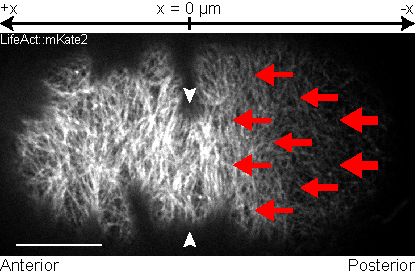
\includegraphics[width=0.7\textwidth]{ActiveMatterModel/FigureModelAC/pcFurrowXYAxis.pdf}
    \caption[Cartesian coordinate system used in model for Pseudocleavage furrow formation]{Cortical section of the \acs{ce} embryo, labelled with LifeAct::mKate2 (white), to depict the organisation of actin filaments at onset of pseudocleavage furrow (white arrows). Red arrows depict anterior-directed cortical flows observed during pseudocleavage furrow onset. The $x$ axis used in \autoref{sec:furrowFormationModelAC} are also depicted, with $x = \SI{0}{\micro\meter}$ at the pseudocleavage furrow, and the posterior (anterior) on the negative (positive) $x$ end. $y$ axis is along the vertical edge of the image. Scale bar: \SI{10}{\micro\meter}. Adapted from \cite{reymann2016cortical}}
    \label{fig:pcFurrowXYAxisModelAC}
\end{figure}

\subsection{Dynamics of Actin alignment}\label{subsec:actinAlignmentModelAC}
Following the discussion in \autoref{sec:introHydrodynamicTheoryActiveFluids}, the constitutive equation that governs the rate of change in the nematic tensor for an active nematic fluid may be written from \autoref{eq:constitutiveEqActiveNematic} as:
\begin{equation}\label{eq:nematicDynamicsGeneralModelAC}
    \frac{DQ_{\alpha\beta}}{Dt} = -\nu \Tilde{v}_{\alpha\beta} + \frac{1}{\bar{\gamma}}H_{\alpha\beta} + \lambda Q_{\alpha\beta}\Delta\mu
\end{equation}
where $\frac{DQ_{\alpha\beta}}{Dt} = \inlinePartial{t}{Q_{\alpha\beta}} + v_\gamma\inlinePartial{\gamma}{Q_{\alpha\beta}} + \omega_{\alpha\gamma}Q_{\gamma\beta} + \omega_{\beta\gamma}Q_{\alpha\gamma}$ is the corotational and comoving derivative of $Q_{\alpha\beta}$ (see \autoref{eq:introCorotateDeriveQ}), $\Tilde{v}_{\alpha\beta} = \frac{\inlinePartial{\alpha}{v_\beta} + \inlinePartial{\beta}{v_\alpha}}{2} - \frac{1}{2}\inlinePartial{\gamma}{v_\gamma}\delta_{\alpha\beta}$ is the traceless symmetric part of the velocity gradient (written for a 2-dimensional cortex, see \autoref{eq:introActiveNematicStrainRate}), $\omega_{\alpha\beta} = \frac{\inlinePartial{\alpha}{v_\beta} - \inlinePartial{\beta}{v_\alpha}}{2}$ is the antisymmetric part of the velocity gradient (see \autoref{eq:introVorticityNematic}), $H_{\alpha\beta} = -\fdv{F_0}{Q_{\alpha\beta}}$ is the molecular field conjugate to the nematic tensor $Q_{\alpha\beta}$ for the instrinsic free energy $F_0$ (see \autoref{eq:introMolecularFieldDefine}) and $\Delta\mu$ is the chemical potential difference for \ac{atp} hydrolysis. Note that the corotational and comoving derivative $\frac{DQ_{\alpha\beta}}{Dt}$ includes the effect of advection on $Q_{\alpha}{\beta}$.

The phenomenological coefficient $\nu$ captures the change in nematic tensor $Q_{\alpha\beta}$ due to the velocity gradient $\Tilde{v}_{\alpha\beta}$ -- thus capturing the compressive alignment of actin filaments driven by flows in the actomyosin cortex. The phenomenological coefficient $\lambda$ couples the activity of myosin motors (which catalyse the hydrolysis of \ac{atp}) to the change in nematic tensor $Q_{\alpha\beta}$ -- thus capturing the active alignment of actin filaments by myosin motors. The phenomenological coefficient $\bar{\gamma}$ captures the relaxation of the actin alignment to the equilibrium state. For the free energy $F_0$, the following form is assumed:
\begin{equation}\label{eq:nematicFreeEnergyModelAC}
    F_0 = K\int\left[\frac{1}{2}Q_{\alpha\beta}Q_{\alpha\beta} + \frac{l^2}{2}\inlinePartial{\gamma}{Q_{\alpha\beta}}\inlinePartial{\gamma}{Q_{\alpha\beta}}\right]\dd{S}
\end{equation}
where the integral is taken over the whole cortex, $K$ characterises the tendency of actin filaments to relax to isotropic orientation ($K > 0$), and $l$ is the characteristic length scale below which filaments are coherently aligned. This form of $F_0$ yields $H_{\alpha\beta}$ as:
\begin{equation}\label{eq:molecularFieldModelAC}
    H_{\alpha\beta} = -\fdv{F_0}{Q_{\alpha\beta}} = K[l^2\inlinePartial{\gamma}{\inlinePartial{\gamma}{Q_{\alpha\beta}}} - Q_{\alpha\beta}]
\end{equation}

Finally, it is noted in \cite{reymann2016cortical} that the active alignment of actin filaments by myosin motors plays an insignificant role in the formation of the pseudocleavage furrow. Thus, $\lambda$ is set to zero. This yields the following equation for the dynamics of $Q_{\alpha\beta}$:
\begin{equation}\label{eq:nematicDynamicsPseudocleavageFurrowModelAC}
    \frac{DQ_{\alpha\beta}}{Dt} = -\nu \Tilde{v}_{\alpha\beta} + \frac{1}{\bar{\gamma}}H_{\alpha\beta} = -\nu \Tilde{v}_{\alpha\beta} + \frac{Kl^2}{\bar{\gamma}}\inlinePartial{\gamma}{\inlinePartial{\gamma}{Q_{\alpha\beta}}} - \frac{K}{\bar{\gamma}}Q_{\alpha\beta}
\end{equation}
As the model assumes the \ac{ap} axis is aligned with the long axis, the rotational symmetry around the long axis can be utilized to neglect derivatives in directions perpendicular to the long axis. Additionally, the component of the cortical flow velocity perpendicular to the long axis is also ignored. This simplifies \autoref{eq:nematicDynamicsPseudocleavageFurrowModelAC} into:
\begin{subequations}\label{eq:nematicDynamicsPseudocleavageFurrowAxiSymmetricModelAC}
    \begin{align}
        \inlinePartial{t}{Q_{xx}} + v_x\inlinePartial{x}{Q_{xx}} &=  -\frac{\nu}{2}\inlinePartial{x}{v_x} + \frac{Kl^2}{\bar{\gamma}}\inlinePartial[2]{x}{Q_{xx}} - \frac{K}{\bar{\gamma}}Q_{xx}\\
        \inlinePartial{t}{Q_{xy}} + v_x\inlinePartial{x}{Q_{xy}} &=  \frac{Kl^2}{\bar{\gamma}}\inlinePartial[2]{x}{Q_{xy}} - \frac{K}{\bar{\gamma}}Q_{xy}
    \end{align}
\end{subequations}
where $x$ denotes the direction along the long axis and $y$ perpendicular to it, on the cortex (see \autoref{fig:pcFurrowXYAxisModelAC}). Note that the curvature of the embryo is not considered in these equations. The nematic tensor is given by:
\begin{equation}
    Q_{\alpha\beta} = \begin{bmatrix} Q_{xx} & Q_{xy}\\ Q_{xy} & -Q_{xx} \end{bmatrix}
\end{equation}
Thus, given the cortical flow velocity $v_x$, \autoref{eq:nematicDynamicsPseudocleavageFurrowAxiSymmetricModelAC} governs the dynamics of the nematic tensor $Q_{\alpha\beta}$ and consequently the alignment of actin filaments in the cortex. At steady state, as assumed in \citep{reymann2016cortical}, $\inlinePartial{t}{Q_{xx}}$ and $\inlinePartial{t}{Q_{xy}}$ are set to zero.

\subsection{Active stress generated by alignment of actin filaments}\label{subsec:activeNematicStressModelAC}
In \cite{reymann2016cortical}, the following form for the stress tensor is proposed:
\begin{equation}\label{eq:totalStressModelAC}
    \sigma_{\alpha\beta} = \eta \Tilde{v}_{\alpha\beta} + \eta_v \inlinePartial{\gamma}{v_\gamma}\delta_{\alpha\beta} + \zeta \delta_{\alpha\beta} + \speciesSuper{\sigma}{nematic}_{\alpha\beta}
\end{equation}
where $\eta$ and $\eta_v$ are shear and bulk viscosity of the cortex respectively. $\zeta$ represents the isotropic part of the active contractile stresses generated by myosin motors in the actomyosin cortex. $\speciesSuper{\sigma}{nematic}_{\alpha\beta}$ is the part of the active tension that depends on the nematic stress tensor $Q_{\alpha\beta}$ -- such a component encodes the anisotropic active stress generated due to the interaction between the myosin motors and aligned actin filaments \citep{reymann2016cortical}. For the purposes of this discussion, the curvature of the embryo is neglected as the primary interest is in the form of the stress tensor. \cite{reymann2016cortical} considers a differential geometry description of the stress tensor, which does include curvature.

The following form of $\speciesSuper{\sigma}{nematic}_{\alpha\beta}$ is proposed:
\begin{equation}\label{eq:nematicStressModelAC}
    \speciesSuper{\sigma}{nematic}_{\alpha\beta} = \frac{\Psi}{2}\left[\frac{1}{\sqrt{2}}\sqrt{Q_{\gamma\nu}Q_{\nu\gamma}}\delta_{\alpha\beta} + Q_{\alpha\beta}\right]
\end{equation}
where $\Psi$ is a phenomenological coefficient that controls the strength of the nematic component of the stress. Note that $\sqrt{Q_{\gamma\nu}Q_{\nu\gamma}}$ is the Frobenius norm of $Q_{\alpha\beta}$. The above form is selected to ensure that the nematic stress is along the local orientation of actin filaments. This can be observed by writing \autoref{eq:introNematicTensorUniaxialDefine} for the 2-dimensional cortex -- with the unit vector $\vec{n}$ denoting the local nematic director (and thus the local orientation of actin filaments):
\begin{align*}
    Q_{\alpha\beta} &= S\left(n_\alpha n_\beta - \frac{1}{2}\delta_{\alpha\beta}\right); \quad n_\alpha n_\alpha = 1\\
    Q_{\alpha\beta}Q_{\beta\alpha} &= S^2\left(n_\alpha n_\beta - \frac{1}{2}\delta_{\alpha\beta}\right)\left(n_\beta n_\alpha - \frac{1}{2}\delta_{\beta\alpha}\right) = \frac{S^2}{2} \implies \sqrt{Q_{\alpha\beta}Q_{\beta\alpha}} = \frac{S}{\sqrt{2}}\\
    \speciesSuper{\sigma}{nematic}_{\alpha\beta} &= \frac{\Psi}{2}\left[\frac{1}{\sqrt{2}}\sqrt{Q_{\gamma\nu}Q_{\nu\gamma}}\delta_{\alpha\beta} + Q_{\alpha\beta}\right] = \frac{\Psi}{2}\left[\frac{S}{2}\delta_{\alpha\beta} + Q_{\alpha\beta}\right] = \frac{S\Psi}{4}n_\alpha n_\beta
\end{align*}
which implies that the stress $\speciesSuper{\sigma}{nematic}_{\alpha\beta}$ will always generate force along the local nematic director $\vec{n}$, never perpendicular to it.

One may also compare the stress tensor used in this section (\autoref{eq:totalStressModelAC}) to those used in the model proposed in \cite{gross2019guiding} (\autoref{eq:totalStressModelPG}) and obtained in the generic theory of active nematic fluids (\autoref{eq:constitutiveEqActiveNematic}):
\begin{itemize}
    \item Comparing to model proposed in \cite{gross2019guiding} and discussed in \autoref{sec:apAxisEstablishModelPG}\hfill\\
    On comparison with \autoref{eq:totalStressModelPG}, one may note that the stress tensor in \autoref{eq:totalStressModelAC} is essentially the same as that in \autoref{eq:totalStressModelPG} plus an additional active term $\speciesSuper{\sigma}{nematic}_{\alpha\beta}$ that arises from the nematic nature of the cortex considered in this section. Note however that the model proposed in \cite{gross2019guiding} ignores the bulk viscosity related terms in the stress, while those are considered here.
    \item Comparing to generic constitutive equations for an active incompressible nematic fluid \citep{julicher2018hydrodynamic} discussed in \autoref{subsec:constitutiveEquationsActiveNematicFluids}\hfill\\
    On comparison with \autoref{eq:constitutiveEqActiveNematic}, one may note that the stress tensor in \autoref{eq:totalStressModelAC} shares the shear viscosity related term $\eta \Tilde{v}_{\alpha\beta}$ with the symmetric deviatoric stress tensor in \autoref{eq:constitutiveEqActiveNematic}. Additionally, the model discussed here contains the bulk viscosity term $\eta_v \inlinePartial{\gamma}{v_\gamma}\delta_{\alpha\beta}$ and active isotropic stress generated by myosin motors $\zeta \delta_{\alpha\beta}$ not considered in \autoref{eq:constitutiveEqActiveNematic}. However such terms are compatible with the generic hydrodynamic theory of active nematic fluid -- as can be observed by comparing the stress tensor for an active isotropic fluid \autoref{eq:introActiveSimpleFluidStress} and active nematic incompressible fluid \autoref{eq:constitutiveEqActiveNematic}. Note that any coupling between isotropic stress and nematic tensor is ignored here. Another difference is the absence of the terms coupling the stress to the molecular field $H_{\alpha\beta}$ and $Q_{\alpha\beta}$ in \autoref{eq:constitutiveEqActiveNematic} -- instead, they are replaced by $\speciesSuper{\sigma}{nematic}_{\alpha\beta}$ in the model discussed in this section. Finally, the equilibrium stress and antisymmetric component of the stress generated in nematic fluids -- as written in \autoref{eq:introActiveNematicDeviatoricStress} -- are ignored here (thus the symmetric traceless deviatoric stress in \autoref{eq:constitutiveEqActiveNematic} is the full stress tensor in \autoref{eq:totalStressModelAC}).
\end{itemize}

\section{A model of \acs{ap} axis alignment in \acs{ce}}\label{sec:apAxisAlignmentModelMN}
In the previous sections, the two models for the actomyosin cortex proposed in \citep{gross2019guiding} and \citep{reymann2016cortical} are discussed. Both studies discussed aspects of the actomyosin cortex during \ac{ap} axis establishment in the one-cell \ac{ce} embryo -- the first discussing the guidance of \ac{ap} axis establishment via centrosomes and the second discussing the formation of the pseudocleavage furrow. In both cases, the \ac{ap} axis is always assumed to be aligned with the long axis of the ellipsoidal embryo. However, as discussed in \autoref{subsec:ApAxisAlignment}, the \ac{ap} axis may not always be aligned with the long axis -- in fact, the \ac{ap} axis actively re-orients to align with the long axis if it is not aligned before. In this section, the theoretical model for this \ac{ap} axis alignment is described -- obtained by combining elements of the two models discussed in \autoref{sec:apAxisEstablishModelPG} and \autoref{sec:furrowFormationModelAC}. This theoretical model is the one used in this thesis for comparison with experimental observations of \ac{ap} axis alignment under different conditions -- see \autoref{ch:Results} for details. This theoretical model of \ac{ap} axis alignment was developed in collaboration with Michael Nestler and Prof. Axel Voigt from the Technische Universit{\"a}t Dresden. The text follows the description in \citep{axisConvergence}.

In the derivation of this theoretical model of the \ac{ap} axis alignment, it is assumed that the fluid flow in the cortex and cytoplasm is laminar -- that is, in the low Reynolds number regime. In this scenario, the inertial terms in the momentum balance for the cortex and cytoplasm can be ignored -- thus, the momemtum balance in the cortex is described by \autoref{eq:momentumBalanceModelPG}, and in the cytoplasm by the Stokes equation. Additionally, it is assumed that the cortical dynamics is fast enough that the \ac{ap} axis alignment may be considered to be a quasi-steady state process. That is, for a given position of the male pronucleus (and thus the centrosomal cues), the concentration of myosin in the cortex and the cortical flow velocity are instantly defined, and can be obtained by the steady state approximation. In effect, the theoretical model of \ac{ap} axis alignment takes as input the given position of the male pronucleus, and calculates as output the velocity of the male pronucleus. In \autoref{ch:Results}, the position of the male pronucleus is recorded as its \enquote{Angular Position}: the angle between the long axis and the line connecting the center of the ellipsoidal embryo to the center of the male pronucleus; and its velocity is recorded as the \enquote{Posteriorisation velocity}: the component of the velocity of the male pronucleus locally parallel to the cortex. 

This section is organised as follows. First, the actomyosin cortex is described as an active nematic surface fluid, on the fixed surface of an ellipsoid. This is achieved in two steps. A bulk description of the cortex as an active nematic compressible fluid is presented -- illustrating the elements of the two models discussed before that are combined here. This bulk description is then converted into a surface description by a thin film limit -- yielding the description of the cortex as an active nematic surface fluid. Note that this description of the cortex takes into account the curvature of the ellipsoid, unlike the two models described in the sections above. Second, the description of the cytoplasmic bulk and transport of the male pronucleus is presented: the cytoplasmic bulk being treated as a Stokes fluid \citep{niwayama2011hydrodynamic} and the male pronucleus as being advected by both cytoplasmic and cortical flows. This description of the cytoplasmic bulk and male pronucleus together with the description of the cortex as an active nematic surface fluid consititutes the theoretical model of \ac{ap} axis alignment considered in this thesis. Finally, the details of the numerical simulations of the theoretical model are presented -- including the details on the calibration of model parameters using experimental data. These numerical simulations were performed by Michael Nestler \citep{axisConvergence}.

\subsection{A thin film active nematic description of the cortex}\label{subsec:cortexModelMN}
Before considering the description of the actomyosin cortex as considered in the theoretical model of \ac{ap} axis alignment, the general constitutive equations for an active compressible nematic fluid can be derived. The description of the actomyosin cortex used in the theoretical model then can be obtained as a special case.

\subsubsection{Constitutive equations for a generic active compressible nematic fluid}
Following the discussion in \autoref{subsec:constitutiveEquationsActiveNematicFluids} and \citep{julicher2018hydrodynamic}, the constitutive equations for the active nematic compressible fluid may be written down. In particular, the entropy production rate may be identified as:
\begin{equation}\label{eq:entropyProductionActiveNematicGenericModelMN}
    T\theta = \Tilde{\sigma}^{d,s}_{\alpha\beta}\Tilde{v}_{\alpha\beta} + \sigma^d\inlinePartial{\gamma}{v_\gamma} + r\Delta\mu + \frac{DQ_{\alpha\beta}}{Dt}H_{\alpha\beta}
\end{equation}
where 
\begin{itemize}
    \item The stress tensor $\sigma_{\alpha\beta}$ is decomposed into a symmetric traceless part $\Tilde{\sigma}^{d,s}_{\alpha\beta}$ and an isotropic stress $\sigma^d$:
    \begin{align*}
        \sigma_{\alpha\beta} &= \Tilde{\sigma}^{d,s}_{\alpha\beta} + \sigma^d\delta_{\alpha\beta}\\
        \Tilde{\sigma}^{d,s}_{\alpha\beta} &= \sigma_{\alpha\beta} - \frac{1}{3}\sigma_{\gamma\gamma}\delta_{\alpha\beta}\\
        \sigma^d &= \frac{1}{3}\sigma_{\gamma\gamma}
    \end{align*}
    Note that the stress tensor is assumed to be symmetric. Additionally, comparison with \autoref{eq:introActiveNematicDeviatoricStress} indicates that the equilibrium stress (along with pressure) and the antisymmetric stress $Q_{\alpha\gamma}H_{\beta\gamma} - H_{\alpha\gamma}Q_{\beta\gamma}$ are ignored, following \cite{reymann2016cortical} (see \autoref{subsec:activeNematicStressModelAC}). 
    \item The velocity gradient $\inlinePartial{\beta}{v_\alpha}$ is decomposed into a symmetric traceless part $\Tilde{v}_{\alpha\beta}$, an antisymmetric part $\omega_{\alpha\beta}$ and an isotropic part $\inlinePartial{\gamma}{v_\gamma}$ ($\vec{v}$ is the cortical flow velocity):
    \begin{align*}
        \inlinePartial{\beta}{v_\alpha} &= \Tilde{v}_{\alpha\beta} + \omega_{\alpha\beta} + \frac{1}{3}\inlinePartial{\gamma}{v_\gamma}\delta_{\alpha\beta}\\
        \Tilde{v}_{\alpha\beta} &= \frac{\inlinePartial{\beta}{v_\alpha} + \inlinePartial{\alpha}{v_\beta}}{2} - \frac{1}{3}\inlinePartial{\gamma}{v_\gamma}\delta_{\alpha\beta}\\
        \omega_{\alpha\beta} &= \frac{\inlinePartial{\beta}{v_\alpha} - \inlinePartial{\alpha}{v_\beta}}{2}
    \end{align*}
    \item $r$ is the reaction rate and $\Delta\mu$ the difference in chemical potential for the \ac{atp} hydrolysis reaction
    \item $H_{\alpha\beta} = -\fdv{F_0}{Q_{\alpha\beta}}$ is the molecular field conjugate to the nematic tensor $Q_{\alpha\beta}$ (see \autoref{eq:introMolecularFieldDefine}), and $\frac{DQ_{\alpha\beta}}{Dt}$ is the corotational and comoving derivative of $Q_{\alpha}{\beta}$ (see \autoref{eq:introCorotateDeriveQ}).
\end{itemize}

\begin{table}[h]
    \centering
    \begin{tabular}{|c|c|c|c|}
        \hline
        Flux $J_n$ & Force $F_n$ & Time reversal signature $\epsilon(J_n), \epsilon(F_n)$ & Rotation symmetry\\
        \hline
        $\Tilde{\sigma}^{d,s}_{\alpha\beta}$ & $\Tilde{v}_{\alpha\beta}$ & 1,-1 & Traceless symmetric tensor\\
        $\sigma^d$ & $\inlinePartial{\gamma}{v_\gamma}$ & 1,-1 & Scalar\\
        $\frac{DQ_{\alpha\beta}}{Dt}$ & $H_{\alpha\beta}$ & -1,1 & Traceless symmetric tensor \\
        $r$ & $\Delta\mu$ & -1,1 & Scalar \\
        \hline
    \end{tabular}
    \caption{Conjugate thermodynamic fluxes and forces for active compressible nematic fluid. Adapted from \cite{julicher2018hydrodynamic}}
    \label{tab:nematicFluidFluxesForcesModelMN}
\end{table}

The conjugate thermodynamic fluxes and forces are identified in \autoref{tab:nematicFluidFluxesForcesModelMN}. Using the Onsager relations and Curie symmetry principle discussed in \autoref{subsec:introIrrevThermoActiveFluids}, the constitutive equations for the active compressible nematic fluid may be written:
\begin{subequations}\label{eq:constitutiveEqActiveNematicGenericModelMN}
    \begin{align}
        \Tilde{\sigma}^{d,s}_{\alpha\beta} &= 2\eta \Tilde{v}_{\alpha\beta} + \chi Q_{\alpha\beta}\inlinePartial{\gamma}{v_\gamma} + \nu H_{\alpha\beta} + \zeta_1 Q_{\alpha\beta}\Delta\mu \\
        \sigma^d &= \chi Q_{\alpha\beta}\Tilde{v}_{\alpha\beta} + \eta_v \inlinePartial{\gamma}{v_\gamma} + \epsilon Q_{\alpha\beta}H_{\alpha\beta} + \zeta_2 \Delta\mu\\
        \frac{DQ_{\alpha\beta}}{Dt} &= -\nu \Tilde{v}_{\alpha\beta} - \epsilon Q_{\alpha\beta}\inlinePartial{\gamma}{v_\gamma} + \frac{1}{\bar{\gamma}} H_{\alpha\beta} + \lambda Q_{\alpha\beta}\Delta\mu\\
        r &= -\zeta_1 Q_{\alpha\beta}\Tilde{v}_{\alpha\beta} - \zeta_2\inlinePartial{\gamma}{v_\gamma} + \lambda Q_{\alpha\beta}H_{\alpha\beta} + \Lambda\Delta\mu
    \end{align}
\end{subequations}
where $\eta, \eta_v, \bar{\gamma}, \Lambda, \chi, \nu, \zeta_1, \epsilon, \zeta_2, \lambda$ are phenomenological coefficients. $\eta$ and $\eta_v$ are the shear and bulk viscosity of the fluid, $\bar{\gamma}$ characterises the relaxation of the local nematic ordering to equilibrium state and $\Lambda$ describes diffusion. $\zeta_1$ and $\zeta_2$ represent active stresses in the fluid -- $\zeta_1$ represnting active nematic stress and $\zeta_2$ representing active isotropic stress. $\lambda$ represents the effect of activity on the nematic tensor -- such as the active alignment of actin filaments by myosin motors \citep{reymann2016cortical} (see \autoref{subsec:actinAlignmentModelAC}). $\nu$ represents the change in nematic tensor due to flows in the fluid -- such as the compressive alignment of actin filaments in the cortex \citep{reymann2016cortical} (see \autoref{subsec:actinAlignmentModelAC}). $\chi$ and $\epsilon$ are additional coefficients that appear in the case of the compressible active nematic fluid, both representing the additional passive stresses generated due to local nematic ordering.

\subsubsection{Bulk description of the actomyosin cortex in the theoretical model of \ac{ap} axis alignment}
\autoref{eq:constitutiveEqActiveNematicGenericModelMN} provides the general constitutive equations that a compressible active nematic fluid follows. However, in the case of the actomyosin cortex, simplifications can be made, following the models described in \autoref{sec:apAxisEstablishModelPG} and \autoref{sec:furrowFormationModelAC}. Note that only the relations related to the stress ($\Tilde{\sigma}^{d,s}_{\alpha\beta}$, $\sigma^d$) and nematic tensor ($\frac{DQ_{\alpha\beta}}{Dt}$) are of interest here. 

Consider the corotational and comoving derivative of $Q_{\alpha\beta}$ first. As described in \cite{reymann2016cortical} (see \autoref{subsec:actinAlignmentModelAC}), the nematic tensor $Q_{\alpha\beta}$ arises due to the alignment of actin filaments. In \citep{reymann2016cortical}, it was shown that for the description of the nematic tensor $Q_{\alpha\beta}$ -- and thus actin alignment -- during the formation of the pseudocleavage furrow, active alignment of actin filaments plays an insignificant role. Thus, $\lambda$ is set to \num{0}. Additionally, \cite{reymann2016cortical} considers an incompressible cortex -- thus implying that $\epsilon$ should also be set to \num{0}. $\frac{DQ_{\alpha\beta}}{Dt}$ is then given by:
\begin{equation}
    \frac{DQ_{\alpha\beta}}{Dt} = -\nu \Tilde{v}_{\alpha\beta} + \frac{1}{\bar{\gamma}}H_{\alpha\beta}
\end{equation}
The form of the intrinsic free energy density $F_0$ is obtained from \cite{reymann2016cortical}. Thus, as discussed in \autoref{subsec:actinAlignmentModelAC}, the molecular field $H_{\alpha\beta}$ is given by:
\begin{equation}
    H_{\alpha\beta} = K[l^2\inlinePartial{\gamma}{\inlinePartial{\gamma}{Q_{\alpha\beta}}} - Q_{\alpha\beta}]
\end{equation}
Furthermore, it is observed that the advection terms in $\frac{DQ_{\alpha\beta}}{Dt}$ only lead to a slight shift in the position of the pseudocleavage furrow. For sake of simplicity, it is assumed here that this advection term can be ignored. In steady state therefore,
\begin{equation}\label{eq:dynamicsNematicsBulkModelMN}
    \frac{DQ_{\alpha\beta}}{Dt} = 0 \implies H_{\alpha\beta} = K[l^2\inlinePartial{\gamma}{\inlinePartial{\gamma}{Q_{\alpha\beta}}} - Q_{\alpha\beta}] = \nu\bar{\gamma} \Tilde{v}_{\alpha\beta}
\end{equation}
This is then the equation (specifically, its surface equivalent, which is discussed later) that governs the dynamics of the nematic tensor $Q_{\alpha\beta}$ in the theoretical model of \ac{ap} axis alignment.

Consider now the isotropic stress $\sigma^d$. Note that the nematic tensor $Q_{\alpha\beta}$ arises due to the local ordering of actin filaments -- and thus the terms $\chi Q_{\alpha\beta}\Tilde{v}_{\alpha\beta}$ and $\epsilon Q_{\alpha\beta} H_{\alpha\beta}$. In here, it is assumed that the isotropic stresses -- that cause expansion or contraction of the local volume elements of the cortex -- are generated solely by myosin motors. Thus, $\chi$ is also set to \num{0} ($\epsilon = \num{0}$ from the previous discussion on dynamics of $Q_{\alpha\beta}$). These assumptions yield:
\begin{equation}
    \sigma^d = \eta_v \inlinePartial{\gamma}{v_\gamma} + \zeta_2 \Delta\mu
\end{equation}
The total stress $\sigma_{\alpha\beta}$ can then be written as:
\begin{equation}
    \sigma_{\alpha\beta} = \Tilde{\sigma}^{d,s}_{\alpha\beta} + \sigma^d\delta_{\alpha\beta} = \left[2\eta \Tilde{v}_{\alpha\beta} + \eta_v \inlinePartial{\gamma}{v_\gamma}\delta_{\alpha\beta} + \nu H_{\alpha\beta}\right] + \left[\zeta_1 Q_{\alpha\beta}\Delta\mu + \zeta_2 \Delta\mu\delta_{\alpha\beta}\right] = \speciesSuper{\sigma}{passive}_{\alpha\beta} + \speciesSuper{\sigma}{active}_{\alpha\beta}
\end{equation}
where $\speciesSuper{\sigma}{passive}_{\alpha\beta} = 2\eta \Tilde{v}_{\alpha\beta} + \eta_v \inlinePartial{\gamma}{v_\gamma}\delta_{\alpha\beta} + \nu H_{\alpha\beta}$ contains the passive terms in the stress and $\speciesSuper{\sigma}{active}_{\alpha\beta} = \zeta_1 Q_{\alpha\beta}\Delta\mu + \zeta_2 \Delta\mu\delta_{\alpha\beta}$ contains the active terms. 

Consider now the passive stress $\speciesSuper{\sigma}{passive}_{\alpha\beta}$. Using \autoref{eq:dynamicsNematicsBulkModelMN} to simplify $\speciesSuper{\sigma}{passive}_{\alpha\beta}$ yields:
\begin{equation}
    H_{\alpha\beta} = \nu\bar{\gamma} \Tilde{v}_{\alpha\beta} \implies \speciesSuper{\sigma}{passive}_{\alpha\beta} = (2\eta +  \nu^2\bar{\gamma})\Tilde{v}_{\alpha\beta} + \eta_v \inlinePartial{\gamma}{v_\gamma}\delta_{\alpha\beta}
\end{equation}
Thus, the stress generated due to compressive alignment of actin filaments $\nu H_{\alpha\beta}$, under the steady state condition assumed in the theoretical model, reduces to an effective renormalization of the viscosity of the cortex. Following \citep{gross2019guiding}, the bulk viscosity is ignored -- that is, $\eta_v$ is set to \num{0}. Then, denoting this effective viscosity as $\Tilde{\eta} = \eta + \frac{\nu^2\bar{\gamma}}{2}$, $\speciesSuper{\sigma}{passive}_{\alpha\beta}$ can be written as:
\begin{equation}
    \speciesSuper{\sigma}{passive}_{\alpha\beta} = 2\Tilde{\eta}\Tilde{v}_{\alpha\beta}
\end{equation}

Consider now the active stress $\speciesSuper{\sigma}{active}_{\alpha\beta}$. Following \cite{gross2019guiding}, the active stress could be written as:
\begin{align}
    \zeta_2 \Delta\mu &= \xi \frac{M}{M + M_*} \\
    \zeta_1 Q_{\alpha\beta}\Delta\mu &= \xi_N \frac{M}{M + M_*} Q_{\alpha\beta}\\
    \speciesSuper{\sigma}{active}_{\alpha\beta} &= \left[\frac{M}{M + M_*}\right](\xi\delta_{\alpha\beta} + \xi_N Q_{\alpha\beta})
\end{align}
where $\xi$ represents the active isotropic stress generated by the cortex, and $\xi_N$ the active anisotropic stress dependent on the local alignment of actin filaments. Here, the dependence of the active stresses on the myosin concentration $M$ is borrowed from \cite{gross2019guiding} -- with $\xi$ and $\xi_N$ playing the role of $C_*$ in \autoref{eq:activeStressModelPG}. Additionally, it is assumed that both isotropic and anisotropic active stress share the same Hill coefficient $M_*$.

In \cite{gross2019guiding}, the dynamics of the myosin concentration $M$ is considered in the context of the reaction-advection-diffusion system of \ac{par} proteins (see \autoref{sec:apAxisEstablishModelPG}). In the theoretical model of \ac{ap} axis alignment considered here, this is simplified to consider only the dynamics of $M$ on the cortex. Specifically, from \autoref{eq:myosinChemicalRateWithCueModelPG}, the term $k_{AM}AM$ that represents the regulation of dissociation of myosin from the cortex by \ac{apar} is not considered here, nor are the dynamics of \ac{apar} and \ac{ppar} in \autoref{eq:allConcDynamicsModelPG}. As the theoretical model considers only steady state, the time component of the centrosomal cue is ignored. Furthermore, the time derivative of $M$ in \autoref{eq:allConcDynamicsModelPG} is ignored. Similar to nematic tensor $Q_{\alpha\beta}$, the advection term for $M$ is also ignored. With these assumptions, the following equation for the dynamics of myosin at the cortex is obtained:
\begin{equation}\label{eq:dynamicsMyosinBulkModelMN}
    -D_M\inlinePartial{\gamma}{\inlinePartial{\gamma}{M}} = k_{on,M}M_{cyto} - k_{off,M}M - k_{off,M}\kappa_MF_M(\vec{r}_{nucl})M
\end{equation}
where $M_{cyto}$ is obtained in a similar fashion to \autoref{eq:concCytoModelPG}, and \\$F_M(\vec{r}_{nucl}) = -\exp(-\frac{\left(\vec{r} - \Pi[\vec{r}_{nucl}]\right)^2}{d_M^2})$ models the centrosomal cue that depletes myosin near the male pronucleus with characteristic length $d_M$. $\vec{r}_{nucl}$ refers to the location of the male pronucleus, and $\Pi[\vec{r}_{nucl}]$ is the point on the cortex closest to the male pronucleus.

The total stress $\sigma_{\alpha\beta}$ is then given by:
\begin{equation}\label{eq:totalStressBulkModelMN}
    \sigma_{\alpha\beta} = \speciesSuper{\sigma}{passive}_{\alpha\beta} + \speciesSuper{\sigma}{active}_{\alpha\beta} = 2\Tilde{\eta}\Tilde{v}_{\alpha\beta} + \xi\left(\frac{M}{M + M_*}\right)\delta_{\alpha\beta} + \xi_N \left(\frac{M}{M + M_*}\right) Q_{\alpha\beta}
\end{equation}
Momentum balance is taken in the Low-Reynolds number regime, following \cite{gross2019guiding}, with a frictional drag coefficient $\gamma$. Thus, \autoref{eq:momentumBalanceModelPG} implies $-\inlinePartial{\beta}{\sigma_{\alpha\beta}} + \gamma v_\alpha = 0$, which yields:
\begin{equation}
    -\Tilde{\eta}\left[\inlinePartial{\beta}{\inlinePartial{\beta}{v_\alpha}} + \frac{1}{3}\inlinePartial{\alpha}{\inlinePartial{\beta}{v_\beta}}\right] + \gamma v_\alpha = \xi\inlinePartial{\alpha}{\left(\frac{M}{M + M_*}\right)} + \xi_N \inlinePartial{\beta}{\left[\left(\frac{M}{M + M_*}\right) Q_{\alpha\beta}\right]}
\end{equation}
Dividing throughout by $\gamma$ yields:
\begin{equation}\label{eq:dynamicsCortexVelocityBulkModelReducedModelMN}
    -\lambda_H\left[\inlinePartial{\beta}{\inlinePartial{\beta}{v_\alpha}} + \frac{1}{3}\inlinePartial{\alpha}{\inlinePartial{\beta}{v_\beta}}\right] + v_\alpha = \lambda_A\inlinePartial{\alpha}{\left(\frac{M}{M + M_*}\right)} + \lambda_N \inlinePartial{\beta}{\left[\left(\frac{M}{M + M_*}\right) Q_{\alpha\beta}\right]}
\end{equation}
where hydrodynamic length $\lambda_H = \frac{\Tilde{\eta}}{\gamma}$, active force relaxation $\lambda_A = \frac{\xi}{\gamma}$ and nematic stress relaxation $\lambda_N = \frac{\xi_N}{\gamma}$ have been introduced. A similar modification can be done for \autoref{eq:dynamicsNematicsBulkModelMN}, yielding:
\begin{equation}\label{eq:dynamicsNematicsBulkModelReducedModelMN}
    l^2\inlinePartial{\gamma}{\inlinePartial{\gamma}{Q_{\alpha\beta}}} - Q_{\alpha\beta} = \nu\tau \Tilde{v}_{\alpha\beta}
\end{equation}
where $\tau = \frac{\bar{\gamma}}{K}$ is the characteristic relaxation time for the nematic tensor $Q_{\alpha\beta}$.

Altogether, the equations \autoref{eq:dynamicsMyosinBulkModelMN}, \autoref{eq:dynamicsCortexVelocityBulkModelReducedModelMN} and \autoref{eq:dynamicsNematicsBulkModelReducedModelMN} constitute the set of dynamical equations that comprise the bulk description of the cortex in the theoretical model. Under the thin film limit discussed next, these equations will be converted into their surface counterparts. Note that the stress induced by nematic ordering in \autoref{eq:totalStressBulkModelMN} -- $\xi_N \left(\frac{M}{M + M_*}\right) Q_{\alpha\beta}$ -- is not the same as that was introduced in \cite{reymann2016cortical}. This will be replaced with the nematic stress introduced in \autoref{eq:nematicStressModelAC} after the thin film limit is applied to obtain a 2-dimensional surface description of the cortex, to ensure that the forces induced by the actin alignment are only along the local orientation of the actin filaments.

\subsubsection{Thin film limit: Description on the surface of an ellipsoid}
The previous section describes the description of the cortex in bulk -- that is, assuming that the cortex is a bulk fluid. However, the actomyosin cortex resides only near the cell membrane -- thus a surface description is needed for the cortex. To transform the bulk description into the relevant surface description, a thin film limit is utilised as described in \citep{nitschke2018nematic}. Let $\mathcal{E}$ denote the surface of the ellipsoidal embryo, and $\hat{\mathcal{E}}$ its interior. Note that the ellipsoidal surface is considered fixed in shape -- the \enquote{ruffling} of the cortex is not considered here. The idea of the thin film limit is to consider a tubular extension $\mathcal{E}_h$ of the surface $\mathcal{E}$ of constant thickness $h$. The bulk description of the cortex considered above is then used in this thin ellipsoidal shell of thickness $h$. By applying proper boundary conditions on this volume $\mathcal{E}_h$ and taking $h \rightarrow 0$, a covariant surface description of the cortex can be obtained.

Denote the outward normal to the surface $\mathcal{E}$, along which the shell $\mathcal{E}_h$ has been extended, as $\vec{n}$. Additionally, in this section tensors will be denoted in boldface. The boundary conditions of the thin shell $\mathcal{E}_h$ are selected as below \citep{nestler2020properties,arroyo2009relaxation,nitschke2020liquid}:
\begin{itemize}
    \item No additional flux of Myosin normal to the cortex beyond what is already considered in the reaction term: $(\nabla M)\cdot\vec{n} = 0$.
    \item No cortical flow along the normal to $\mathcal{E}$, and thus the boundary of $\mathcal{E}_h$: $\vec{v}\cdot\vec{n} = 0$.
    \item No variation in cortical flow velocity along the normal to $\mathcal{E}$, and thus between the outer and inner boundary of $\mathcal{E}_h$: $(\vec{n}\cdot\nabla)\vec{v} = 0$.
    \item No nematic ordering in the direction normal to $\mathcal{E}$: $\vec{n}\cdot\mathbf{Q}\cdot\vec{n} = 0$. Additionally, it is assumed that $(\nabla\mathbf{Q})\cdot\vec{n} = 0$, to ensure continous values for $\mathbf{Q}$ as $h \rightarrow 0$ \citep{nestler2020properties}.
    \item Normal components of the stress do not contain tangential parts and vice-versa: $\mathbf{\sigma}\cdot\vec{n}$ is a vector along $\vec{n}$. Under this condition, the tangential and normal (to the surface $\mathcal{E}$) parts of the stress decouple. Note that this also implies that only the tangential parts of the stress tensor are considered in the theoretical model.
\end{itemize}
Note that since $h \rightarrow 0$, it has been assumed that the normal vector to the surface of $\mathcal{E}_h$ does not vary much from the corresponding normal vector to the surface $\mathcal{E}$.

With these considerations, the dynamic equations of the theoretical model -- \autoref{eq:dynamicsMyosinBulkModelMN}, \autoref{eq:dynamicsCortexVelocityBulkModelReducedModelMN} and \autoref{eq:dynamicsNematicsBulkModelReducedModelMN} -- can be converted into a covariant surface form after applying the thin film limit. Here, only the tangential parts of the corresponding tensors in the bulk description are considered. Additionally, the covariant gradient and divergence operations on the surface $\mathcal{E}$ are denoted by $\gradSurf$ and $\divSurf$ respectively. Here, the surface equations are directly reported -- the reader is referred to \citep{axisConvergence} for details.

The dynamics of myosin concentration $M$ on the cortex is governed by:
\begin{equation}\label{eq:dynamicsMyosinSurfaceModelMN}
    -D_M \divSurf\gradSurf M = k_{on,M}M_{cyto} - k_{off,M}M - k_{off,M}\kappa_MF_M(\vec{r}_{nucl})M
\end{equation}
where $M_{cyto} = M_{tot} - \frac{\psi}{\abs{\mathcal{E}}}\int_\mathcal{E} M \dd{\mathcal{E}}$ -- as in \autoref{eq:concCytoModelPG} and $F_M(\vec{r}_{nucl}) = -\exp(-\frac{s(\vec{r},\Pi[\vec{r}_{nucl}])^2}{d_M^2})$ where $s$ is the geodesic distance measure on $\mathcal{E}$ and $\Pi[\vec{r}_{nucl}]$ is the closest point on the cortex with respect to the male pronucleus center. $\mathbf{g}$ denotes the metric of the ellipsoid surface $\mathcal{E}$.

The dynamics of the nematic tensor $\mathbf{Q}$ on the cortex is governed by \citep{nitschke2018nematic}:
\begin{equation}\label{eq:dynamicsNematicsSurfaceModelMN}
    l^2[\divSurf\gradSurf\mathbf{Q} - \norm{\mathbf{B}}^2\mathbf{Q}] - \mathbf{Q} = \nu\tau \mathbf{\Tilde{v}}
\end{equation}
where $\mathbf{B} = -\Pi[\nabla\vec{n}]$ is the shape operator of $\mathcal{E}$ -- that is, the projection (to the tangent space of $\mathcal{E}$, denoted by $\Pi$) of the gradient of the normal vector $\vec{n}$ of $\mathcal{E}$. $\mathbf{Q}$ is the nematic tensor and $\mathbf{\Tilde{v}} = \frac{1}{2}[\gradSurf\vec{v} + (\gradSurf\vec{v})^T - (\divSurf\vec{v})\mathbf{g}]$ is the symmetric traceless strain rate, both tangential to the surface $\mathcal{E}$. Note that the determinant of the shape operator $\mathbf{B}$ is the gaussian curvature $\mathcal{K}$.

The momentum balance for the cortex in this surface description reads:
\begin{equation*}
    -\lambda_H\left[\divSurf\gradSurf\vec{v} + \mathcal{K}\vec{v} + \frac{1}{3}\gradSurf\divSurf\vec{v}\right] + \vec{v} = \lambda_A\gradSurf\left(\frac{M}{M + M_*}\right) + \lambda_N \divSurf\left[\left(\frac{M}{M + M_*}\right) \mathbf{Q}\right]
\end{equation*}
where $\vec{v}$ is the cortical flow velocity and the rest are defined in \autoref{eq:dynamicsCortexVelocityBulkModelReducedModelMN}. As noted before, the form of the stress induced by actin alignment is not in the form presented in \autoref{eq:nematicStressModelAC}. Replacing the nematic stress here to that from \autoref{eq:nematicStressModelAC} yields:
\begin{equation*}
    \left(\frac{M}{M + M_*}\right) \mathbf{Q} \rightarrow \left(\frac{M}{M + M_*}\right)\left[\frac{1}{2\sqrt{2}}\norm{\mathbf{Q}}\mathbf{g} + \frac{1}{2}\mathbf{Q}\right]
\end{equation*}
\begin{multline}\label{eq:dynamicsCortexVelocitySurfaceModelMN}
    -\lambda_H\left[\divSurf\gradSurf\vec{v} + \mathcal{K}\vec{v} + \frac{1}{3}\gradSurf\divSurf\vec{v}\right] + \vec{v} \\= \lambda_A\gradSurf\left(\frac{M}{M + M_*}\right) + \lambda_N \gradSurf\left[\left(\frac{M}{M + M_*}\right)\left(\frac{1}{2\sqrt{2}}\norm{\mathbf{Q}}\mathbf{g} + \frac{1}{2}\mathbf{Q}\right)\right]    
\end{multline}
where $\mathbf{g}$ is the metric of the ellipsoid surface $\mathcal{E}$.

Altogether, the equations \autoref{eq:dynamicsMyosinSurfaceModelMN}, \autoref{eq:dynamicsNematicsSurfaceModelMN} and \autoref{eq:dynamicsCortexVelocitySurfaceModelMN} constitute the set of dynamical equations that comprise the surface description of the cortex -- the description of the cortex that is used in the theoretical model of \ac{ap} axis alignment.

A note may be made on the parameters \hydrodynamicLength, \activeRelaxLength and \nematicLength in \autoref{eq:dynamicsCortexVelocitySurfaceModelMN}. These parameters characterise the strength of the passive and active stresses in the cortex relative to frictional drag -- with \hydrodynamicLength characterising the passive viscous stress, \activeRelaxLength characterising the active isotropic stress and \nematicLength characterising the active anisotropic stress generated by the local alignment of actin filaments. As discussed in \cite{reymann2016cortical}, this anisotropic stress generated by alignment of actin filaments gives rise to the contractile ring-like nature of the pseudocleavage furrow that forms during the late establishment phase. The active isotropic stress characterised by \activeRelaxLength cannot generate such a ring-like structure. Furthermore, as discussed in \cite{niwayama2011hydrodynamic}, this active isotropic stress can capture the cytoplasmic flows observed in the cytoplasm. Thus, \nematicLength controls the strength of active anisotropic stress generated in the cortex by the pseudocleavage furrow; while \activeRelaxLength controls the strength of the isotropic active stress in the cortex. In other words, \nematicLength controls the strength of the pseudocleavage furrow-dependent mechanism, while \activeRelaxLength controls the strength of the cytoplasmic flow-dependent mechanism discussed in \autoref{subsec:ApAxisAlignment}.

\subsection{Description of the Cytoplasm and Male pronucleus}\label{subsec:cytoplasmPronucleusModelMN}

\subsubsection{Flows in the cytoplasmic bulk}
Following the results of \cite{niwayama2011hydrodynamic}, the cytoplasmic bulk can be modelled as an incompressible Newtonian fluid in the Stokes regime, with flows in it driven by flows at the cortex. Specifically, the flow in the cytoplasmic bulk $\hat{\mathcal{E}}$ is given by the Stokes equation:
\begin{equation}\label{eq:stokesModelMN}
    \nabla\cdot\left(\eta_{cyto}\nabla\vec{v}_{cyto}\right) - \nabla p = 0; \quad \nabla\cdot\vec{v}_{cyto} = 0 \quad \textrm{in }\hat{\mathcal{E}}
\end{equation}
where $\eta_{cyto}$ is cytoplasmic viscosity, $\vec{v}_{cyto}$ is the flow velocity of the cytoplasm and $p$ is the pressure in the cytoplasm. 

Following the approach in \citep{tanaka2000simulation}, the male pronucleus itself is treated as a colloidal particle in the cytoplasm. Specifically, the male pronucleus is modelled as a region $\phi(\vec{r})$ with a large viscosity $\omega_{nucl}\eta_{cyto}$ in the cytoplasm to ensure homogeneous flow field inside the pronucleus region:
\begin{equation}
    \phi(\vec{r}) = \frac{1}{2}\left[1- \tanh(\frac{3\left(\norm{\vec{r} - \vec{r}_{nucl}} - R_{nucl}\right)}{\bar{\epsilon}})\right]; \quad \vec{r} \in \hat{\mathcal{E}}
\end{equation}
where $\vec{r}_{nucl}$ is the center of the male pronucleus, $R_{nucl}$ is the radius of the male pronucleus and $\bar{\epsilon}$ the width of transition of this function from \num{0} to \num{1} -- usually selected to be small. The viscosity term in \autoref{eq:stokesModelMN} is then replaced $\eta_{cyto} \rightarrow \eta_{cyto}(1 + \omega_{nucl}\phi(\vec{r}))$ \citep{tanaka2000simulation}. Dividing throughout by $\eta_{cyto}$ and setting $\bar{p} = \flatfrac{p}{\eta_{cyto}}$ yields the dynamical equations for the cytoplasmic flow velocity $\vec{v}_{cyto}$ as:
\begin{subequations}\label{eq:cytoFlowModelMN}
    \begin{align}
        \nabla\cdot\left((1 + \omega_{nucl}\phi(\vec{r}))\nabla\vec{v}_{cyto}\right) - \nabla \bar{p} = 0 & \quad \textrm{in }\hat{\mathcal{E}}\\
        \nabla\cdot\vec{v}_{cyto} = 0 & \quad \textrm{in }\hat{\mathcal{E}}\\
        \vec{v}_{cyto} = \vec{v} & \quad \textrm{on }\partial\hat{\mathcal{E}} = \mathcal{E}
    \end{align}
\end{subequations}
where the last equation specifics the no-slip boundary condition for the cytoplasmic flow velocity at the cortex.

\subsubsection{Posteriorisation velocity of the male pronucleus}
The velocity of the male pronucleus is then calculated from two contributions: advective transport by cytoplasmic flows and drag on the pronucleus due to local movement of the cortex. To obtain the first contribution, the cytoplasmic flow velocity $\vec{v}_{cyto}$ observed in the domain of the pronucleus $\phi(\vec{r})$ is averaged. 
\begin{equation*}
    \speciesSuper{\vec{v}}{cyto}_{nucl} = \frac{\int_{\hat{\mathcal{E}}} \phi(\vec{r})\vec{v}_{cyto} \dd{\hat{\mathcal{E}}}}{\int_{\hat{\mathcal{E}}} \phi(\vec{r}) \dd{\hat{\mathcal{E}}}}
\end{equation*}
The second contribution is obtained by averaging the cortical flow velocity $\vec{v}$ over a domain $\mathcal{N}$ matching the projection of the male pronucleus, centered around the point $\Pi[\vec{r}_{nucl}]$ on $\mathcal{E}$ -- the point on the cortex closest to the center of the male pronucleus $\vec{r}_{nucl}$.
\begin{equation*}
    \mathcal{N} = \{\vec{r} \in \mathcal{E} : s(\vec{r},\Pi[\vec{r}_{nucl}]) \leq R_{nucl} \};\quad \speciesSuper{\vec{v}}{crtx}_{nucl} = \frac{\int_{\mathcal{N}} \vec{v} \dd{\mathcal{N}}}{\abs{N}}
\end{equation*}
where $s$ is the geodesic distance measure on $\mathcal{E}$, $\Pi[\vec{r}_{nucl}]$ is the closest point on the cortex with respect to the male pronucleus center and $R_{nucl}$ is the radius of the male pronucleus. 

The total velocity of the male pronucleus is then given by:
\begin{equation}\label{eq:pronucleusTransportModelMN}
    \vec{v}_{nucl} = \speciesSuper{\vec{v}}{cyto}_{nucl}  + d\,\speciesSuper{\vec{v}}{crtx}_{nucl} 
\end{equation}
where $d \in [0,1]$ is a phenomenological coefficient that characterises the strength of the drag on the pronucleus due to local movement of the cortex. The posteriorisation velocity $\speciesSuper{\vec{v}}{post}_{nucl}$ is then obtained as the component of $\vec{v}_{nucl}$ parallel to $\mathcal{E}$, using the unit normal vector $\vec{n}$ to $\mathcal{E}$ at $\Pi[\vec{r}_{nucl}]$  :
\begin{equation}\label{eq:pronucleusPostVelModelMN}
    \speciesSuper{\vec{v}}{post}_{nucl} = \vec{v}_{nucl} - (\vec{v}_{nucl}\cdot\vec{n})\vec{n}
\end{equation}

\subsection{Numerical simulations of the theoretical model}\label{subsec:numericsModelMN}
The previous paragraphs describe the development of the theoretical model of \ac{ap} axis alignment, which will be used in \autoref{ch:Results} to compare against and make predictions about experimentally observed \ac{ap} axis alignment in \ac{ce} embryos. Conceptually, this model describes how flows in the actomyosin cortex drive flows in the cytoplasm and the subsequent displacement of the male pronucleus. As discussed in \autoref{sec:ApAxisEstablishment}, the male pronucleus acts as the organiser of \ac{ap} axis establishment (via the centrosomes associated with the male pronucleus). Thus, the theoretical model captures how cortical flows drive the re-orientation of the \ac{ap} axis as it aligns with the long axis of the ellipsoidal embryo. 

In this theoretical model, dynamics of the actomyosin cortex is described by integrating elements from the models proposed in \cite{gross2019guiding} and \cite{reymann2016cortical} into a generic hydrodynamic theory of active nematic compressible fluid; and then made into a surface description using a thin film limit \citep{nitschke2018nematic}. For a given position of the male pronucleus $\vec{r}_{nucl}$ in the cytoplasm $\hat{\mathcal{E}}$, the spatial pattern of myosin concentrations $M$ on the cortex $\mathcal{E}$ is determined by \autoref{eq:dynamicsMyosinSurfaceModelMN} -- where $F_M(\vec{r}_{nucl}) = -\exp(-\frac{s(\vec{r},\Pi[\vec{r}_{nucl}])^2}{d_M^2})$ represents the polarisation cue from the centrosomes associated with the male pronucleus. Given these concentrations, the coupled equations \autoref{eq:dynamicsNematicsSurfaceModelMN} and \autoref{eq:dynamicsCortexVelocitySurfaceModelMN} determine the cortical flow velocity $\vec{v}$ and nematic tensor $\mathbf{Q}$ characterising the local state of alignment of actin filaments in the cortex. Myosin dynamics, centrosomal cue and dependence of active stresses on myosin concentration are borrowed from \cite{gross2019guiding}. Active stress generated by nematic tensor (included in \autoref{eq:dynamicsCortexVelocitySurfaceModelMN}) -- and therefore the alignment of actin filaments -- and the compressive alignment of actin filaments (included in \autoref{eq:dynamicsNematicsSurfaceModelMN}) are borrowed from \cite{reymann2016cortical}. These cortical flow determine the flows in the cytoplasm via a no-slip boundary condition at the interface between the cortex and the cytoplasm in \autoref{eq:cytoFlowModelMN}, in which the cytoplasm is assumed to be a Newtonian fluid in the Stokes regime. The effect of the flows in the bulk cytoplasm on the cortex are captured already in the frictional drag in \autoref{eq:dynamicsCortexVelocitySurfaceModelMN}. Finally, the velocity of the male pronucleus is calculated as a summation of two contributions from \autoref{eq:pronucleusTransportModelMN} -- one due to advection by cytoplasmic flows, and the other due to drag with the moving cortex. Thus, the theoretical model describes a feedback loop between the position of the male pronucleus and its velocity, which is governed by the geometry of the embryo via its effect on the cortical and cytoplasmic flow fields.

The numerical simulations of the theoretical model use the \enquote{one-way} description of the previous paragraph, in effect calculating the velocity of the male pronucleus for a given position of the male pronucleus. Specifically, the numerical simulations take as input the angular position $\alpha$ of the male pronucleus -- the angle made between the long axis of the ellipsoidal embryo and line connecting the center of the male pronucleus and the center of the embryo. Assuming a constant distance between the cortex and male pronucleus $\norm{\vec{r}_{nucl} - \Pi[\vec{r}_{nucl}]} = \SI{3.5}{\unitLength}$ and a nucleus radius $R_{nucl} = \SI{3}{\unitLength}$, the corresponding $\vec{r}_{nucl}$ can be recovered from the angular position $\alpha$. Angular positions $\alpha$ are selected between \SIrange{0}{20}{\unitAngle}. For each angular position, the corresponding cortical flow velocity $\vec{v}$ and nematic tensor $\mathbf{Q}$ are calculated by solving \autoref{eq:dynamicsMyosinSurfaceModelMN}, \autoref{eq:dynamicsNematicsSurfaceModelMN} and \autoref{eq:dynamicsCortexVelocitySurfaceModelMN} using surface finite element methods for tangential vector and tensor quantities \citep{Nestler_JCP_2019}. The corresponding cytoplasmic flow velocity $\vec{v}_{cyto}$ are calculated using standard finite element methods, with boundary conditions on the cytoplasm imposed using a diffuse domain approach \citep{Li_CMS_2009}. Using these, the velocity of the male pronucleus $\vec{v}_{nucl}$, and thus the posteriorisation velocity $\speciesSuper{\vec{v}}{post}_{nucl}$ using \autoref{eq:pronucleusPostVelModelMN}, can be calculated for each angular position $\alpha$. All finite element methods are implemented and solved using the AMDiS toolbox.
\subsubsection{Calibrating model parameters}
One may observe that there are several parameters whose values are required before the numerical simulations outlined above can be performed. Specifically, the following model parameters are required: 
\begin{itemize}
    \item Parameters for myosin concentration (\autoref{eq:dynamicsMyosinSurfaceModelMN}): $D_M; k_{on,M}; k_{off,M}; \kappa_M; d_M$. These parameters can be directly obtained from \cite{gross2019guiding}.
    \item Parameters for actin alignment (\autoref{eq:dynamicsNematicsSurfaceModelMN}): $l;\nu\tau$. These can be obtained from \cite{reymann2016cortical}.
    \item Parameters for cortical flow velocity (\autoref{eq:dynamicsCortexVelocitySurfaceModelMN}): $M_*$;\hydrodynamicLength;\nematicLength;\activeRelaxLength. Of these only $M_*$ can be obtained, from \cite{gross2019guiding}.
    \item Parameters for cytoplasmic flow velocity (\autoref{eq:cytoFlowModelMN}): $\omega_{nucl}; \bar{\epsilon}; R_{nucl}$. Note that $\omega_{nucl}; \bar{\epsilon}$ are numeric parameters -- with no physical relevance. $\omega_{nucl}$ is only required to be $\omega_{nucl} >> 1$ to ensure the required behaviour of a homogeneous flow field inside the pronucleus region $\phi(\vec{r})$; $\bar{\epsilon}$ is only required to be $\bar{\epsilon} << R_{nucl}$ to ensure a sharp transition between the pronucleus and cytoplasm. Here, $R_{nucl} = \SI{3}{\unitLength}$, $\bar{\epsilon} = \SI{0.25}{\unitLength}$ and $\omega_{nucl} = \num{100}$ is chosen.
    \item Parameters for pronucleus velocity (\autoref{eq:pronucleusTransportModelMN}): \dragCoefficient
\end{itemize}
Thus, most of the model parameters are already determined in \citep{gross2019guiding} and \citep{reymann2016cortical} -- see \autoref{tab:prevWorkModelParameters} for the their values. Only \num{4} parameters need to be determined: \hydrodynamicLength, \nematicLength, \activeRelaxLength and \dragCoefficient. Of these, the first three -- \hydrodynamicLength, \nematicLength and \activeRelaxLength -- are determined by matching the cortical flows calculated by the theoretical model with those observed in experiments. This \enquote{calibration} of the model is described next. \dragCoefficient is determined by fitting the observed posteriorisation velocity as a function of angular position for the unperturbed embryos only -- see \autoref{subsec:expVsTheoryPcFurrow} for details.

\begin{table}[h]
    \centering
    \begin{tabular}{|c|C{0.35\textwidth}|c|c|}
        \hline
        Model Parameter & Physical revelance & Parameter Value & Source\\
        \hline
        \hline
        $D_M$ & Myosin diffusion constant on cortex & \SI{0.054}{\micro\meter\squared\per\second} & \citep{gross2019guiding}\\
        $k_{on,M}$ & Myosin association rate with cortex & \SI{0.20}{\micro\meter\per\second} & \citep{gross2019guiding}\\
        $k_{off,M}$ & Myosin dissociation rate from cortex & \SI{0.12}{\per\second} & \citep{gross2019guiding}\\
        $\kappa_M$ & Strength of polarity cue (myosin depletion) & \num{4.9} & \citep{gross2019guiding}\\
        $d_M$ & Characteristic length for polarity cue (myosin depletion) & \SI{15.9}{\micro\meter} & \citep{gross2019guiding}\\
        $M_*$ & Hill coefficient for contractility & \SI{8.0}{\per\micro\meter\squared} & \citep{gross2019guiding}\\
        \hline
        $l$ & Length scale below which actin filaments are coherently aligned & \SI{4.72}{\micro\meter} & \citep{reymann2016cortical}\\
        $\nu\tau$ & Compressive alignment of actin filaments & \SI{0.63}{\minute} & \citep{reymann2016cortical}\\
        \hline
        $\omega_{nucl}$ & Numeric parameter & \num{100} & See \citep{tanaka2000simulation}\\
        $\bar{\epsilon}$ & Numeric parameter & \SI{0.25}{\micro\meter} & -\\
        $R_{nucl}$ & Radius of Male pronucleus & \SI{3}{\micro\meter} & \citep{mirna2015linking}\\
        \hline
    \end{tabular}
    \caption{Values of model parameter used in the theoretical model which are not obtained by calibration. Both $\omega_{nucl}$ and $\bar{\epsilon}$ are numeric parameters that do not have physical relevance. See text for explanation. For $R_{nucl}$, also see \autoref{sec:imageAnalysis}}
    \label{tab:prevWorkModelParameters}
\end{table}

To determine the values of \hydrodynamicLength, \nematicLength and \activeRelaxLength, the calibration procedure matches the calculated cortical flows in the numerical simulations to those observed in experiments. These experimental cortical flow fields are measured from the midplane images of the embryo -- thus available only on a planar slice $\mathcal{P}$ -- for a range of different angular positions of the male pronucleus (see \autoref{subsec:corticalFlows} and \autoref{sec:statAnalysis}). The experimental cortical flow velocity is described as a function of arclength $s$ along this planar slice $\mathcal{P}$, with the posterior end designated as the origin and oriented along the counter-clockwise direction (represented by the tangent vector $\vec{t}$ pointing counter-clockwise). For calibration, the experiment cortical flows are shifted to have the closest point to the male pronucleus on $\mathcal{P}$ as the origin.

One may observe that the cortical velocity $\vec{v}$ and nematic tensor $\mathbf{Q}$ in \autoref{eq:dynamicsCortexVelocitySurfaceModelMN} scale with \activeRelaxLength -- that is, $\tilde{C} \lambda_A \rightarrow (\tilde{C}\vec{v}, \tilde{C}\mathbf{Q})$. Using this, \activeRelaxLength can be independently fit by matching the kinetic energy of the calculated and experimental cortical flows. With this, the calibration then proceeds in two steps:
\begin{enumerate}
    \item \autoref{eq:dynamicsMyosinSurfaceModelMN}, \autoref{eq:dynamicsNematicsSurfaceModelMN} and \autoref{eq:dynamicsCortexVelocitySurfaceModelMN} are solved for different values of \hydrodynamicLength and \nematicLength while keeping $\lambda_A^*$ fixed. This solution yields the myosin concentration $M$, and scaled version of the cortical flow velocity $\vec{v}^*$ and nematic tensor $\mathbf{Q}^*$. To obtain the proper scaling, the kinetic energy $\mathbb{E}^\mathcal{P}(\vec{v}) = \int_\mathcal{P} \vec{v}^2 \dd{\mathcal{P}}$ is fit across all angular positions:
    \begin{equation*}
        \min_{S \in \mathbb{R}}\sum_\alpha \left[ \mathbb{E}^\mathcal{P}(\speciesSuper{\vec{v}}{\textrm{expt}}) - \mathbb{E}^\mathcal{P}(S\vec{v}^*) \right] = S^*
    \end{equation*}
    where the summation goes over all angular positions for which experimental cortical flows $\speciesSuper{\vec{v}}{\textrm{expt}}$ are available. As the scaled cortical flow velocity $\vec{v}^*$ are calculated for a selected value of \hydrodynamicLength and \nematicLength, $S^*$ is thus a function of \hydrodynamicLength and \nematicLength. Therefore, for a given value of \hydrodynamicLength and \nematicLength, $\lambda_A = S^*\lambda_A^*$, $\vec{v} = S^*\vec{v}^*$ and $\mathbf{Q} = S^*\mathbf{Q}^*$ are obtained as best match to experimentally measured cortical flows. 
    \item To obtain the values of \hydrodynamicLength and \nematicLength that best match the experimentally measured cortical flows, a mixed calibration cost measure $E = L + \Theta R$ -- combining a similarity measure $L$ and an imbalance measure $R$ with weighting factor $\Theta$ -- is evaluated. The measures $L$ and $R$ are defined as \citep{axisConvergence}:
    \begin{align*}
        L &= \sum_\alpha \sqrt{\frac{\mathbb{E}^\mathcal{P}(\speciesSuper{\vec{v}}{\textrm{expt}}) - \mathbb{E}^\mathcal{P}(\vec{v})}{\mathbb{E}^\mathcal{P}(\vec{v})}} \\
        M^+(\vec{v}) &= -\frac{1}{2}\int_{\mathcal{P}} (-\vec{v}\cdot\vec{t} - \abs{\vec{v}\cdot\vec{t}}) \dd{\mathcal{P}} \\
        M^-(\vec{v}) &= -\frac{1}{2}\int_{\mathcal{P}} (\vec{v}\cdot\vec{t} - \abs{\vec{v}\cdot\vec{t}}) \dd{\mathcal{P}}\\
        R = & \sum_\alpha \flatfrac{\abs{\frac{M^+(\speciesSuper{\vec{v}}{\textrm{expt}})}{M^-(\speciesSuper{\vec{v}}{\textrm{expt}})} - \frac{M^+(\vec{v})}{M^-(\vec{v})}}}{\abs{\frac{M^+(\vec{v})}{M^-(\vec{v})}}} 
    \end{align*}
    where the summation goes over all angular positions for which experimental cortical flows $\speciesSuper{\vec{v}}{\textrm{expt}}$ are available. The similarity measure $L$ penalizes the mismatch between the kinetic energy of the cortical flows calculated in simulations and experimentally measured cortical flows. $M^+$ is the sum of magnitude of flow velocities pointed counter-clockwise, and $M^-$ is the sum of magnitude of flow velocities pointed clockwise. The ratio $\flatfrac{M^+}{M^-}$ thus characterises the \enquote{imbalance} in the cortical flow field. The imbalance measure $R$ penalizes the mismatch for this imbalance between the cortical flows calculated in simulations and experimentally measured cortical flows. Both $L$ and $R$ are considered relative to the calculated cortical flow velocity. This imbalance measure is motivated by the observation of a correlation between the angular position and the imbalance in the experimentally observed flow fields. $\Theta$ weighs the importance of matching the imbalance observed in experimental flow fields -- and is set to $\Theta = 5$.
\end{enumerate}

\subsubsection{Evaluating male pronucleus trajectories}
Trajectories of the male pronucleus -- that is, the angular position as a function of time $\alpha(t)$ -- are evaluated by integrating the calculated velocity of the male pronucleus \autoref{eq:pronucleusPostVelModelMN}, for an initial angular position set at $\alpha = \SI{45}{\unitAngle}$ and arbitrary time domain $t \in [0,1000]$. For comparison with experimentally observed trajectories of the male pronucleus (see \autoref{ch:Results}), a temporal reference point $\hat{t}$ is introduced -- separately defined for each experimental condition. For each experimental conditions, the experimentally obtained trajectories are binned temporally (using \num{100} bins). $\hat{t}$ is then selected using least square, to ensure best fit to experimentally observed trajectories:
\begin{equation*}
    \min_{\hat{t} \in \mathbb{R}} \sum_{i=1}^{100} \abs{\speciesSuper{\alpha}{\textrm{expt}}(t_i) - \alpha(t_i - \hat{t})}^2 \rightarrow \hat{t}
\end{equation*}

\chapter{Materials and Methods}\label{ch:Exp}
\section{Culture conditions, strains and worm handling}\label{sec:wormHandling}
\acs{ce} worms were cultured on \ac{ngm} agar plates seeded with OP50 \ac{ecoli} (a slow-growing \ac{ecoli} bacterial strain), and handled as described in \cite{brenner1974genetics}. Worms were maintained at \SI{20}{\celsius}. The following strains were used in this work:

\begin{table}[h!]
    \centering
    \begin{tabular}{| c | c | m{0.4\textwidth} |} 
        \hline
        Strain & Fluorescent tags & \hfil Genotype \\
        \hline
        SWG070 & \flurophoreLabel{\ac{nmy2}}{\ac{gfp}}, \flurophoreLabel{phDomain}{mCherry} & nmy-2(cp7[nmy-2::gfp + LoxP unc-119(+) LoxP]) I; ltIs44 [pAA173 pie-1p-mCherry::PH(PLC1delta1) + unc-119(+)]\\[3em]
        SWG057 & \flurophoreLabel{\ac{tub}}{\ac{gfp}}, \flurophoreLabel{\ac{nmy2}}{mKate} & nmy-2(cp52 [nmy-2::mkate2 + LoxP unc-119(+) LoxP]) I;  unc-119(ed3)III; ruIs57[pAZ147: pie-1p/GFP::C36E8.5] III\\[3em]
        SWG228 & \flurophoreLabel{\ac{nmy2}}{\ac{gfp}} & nmy-2(cp8[nmy-2::GFP]) I; nop-1(it142) III\\
        \hline
    \end{tabular}
    \caption{\ac{ce} strains used in this study}
    \label{tab:ceStrains}
\end{table}

The primary strain used in this work is a dual-color strain labelled with \flurophoreLabel{\ac{nmy2}}{\ac{gfp}} and \flurophoreLabel{phDomain}{mCherry}, named SWG070. This transgenic strain labels \ac{nmy2} myosin with \acf{gfp} and PH-domain (localized to the cell membrane \citep{park2008comprehensive}) with mCherry (a red fluorescent protein \citep{shaner2004improved}). Thus, SWG070 enable visualization of the myosin distributions in the embryo and its cell membrane during its development. SWG228 is the \geneExp{nop-1} mutant strain used primarily for the triple \geneExp{air-1; mel-11} in \geneExp{nop-1} mutant background (see \autoref{subsec:sufficiencyTestAir1}). For experiments with \geneExp{goa-1; gpa-16} double \ac{rnai} (see \autoref{subsec:MicrotubuleRoleGoa1Gpa16}), SWG057 was used. This strain labels tubulin with \ac{gfp} and \ac{nmy2} myosin with mCherry. This allows visualization of the centrosomes in this condition, required for evaluating if the double \ac{rnai} was successful. 

\section{Genetic perturbations by \acs{rnai}}\label{sec:rnaiMethods}
In order to achieve specific effects (example: embryos deficient in pseudocleavage furrow), expression of specific genes is reduced via \acl{rnai} (example: NOP-1). All \acf{rnai} experiments were performed via feeding, as previously described \citep{timmons2001ingestion,kamath2003genome}. For this process, \ac{rnai} feeding plates were generated by seeding \ac{ngm} agar plates, containing \SI{1}{\milli\Molar} isopropyl-$\beta$-D-thiogalactoside and \SI{50}{\micro\gram\per\milli\liter} ampicillin, with the bacterial expressing the \ac{dsRNA} targeting the gene of interest, and grown overnight. \ac{rnai} was then performed by transferring young L4 worms onto these \ac{rnai} feeding plates and incubating them for the specified time at \SI{20}{\celsius} before imaging. See \autoref{tab:RNAiTime} for incubation times used. For single \ac{rnai} interference experiments, only the \ac{rnai} clone of interest was grown on the \ac{rnai} feeding plates. For double \ac{rnai} of \geneExp{nop-1; mel-11} and double \ac{rnai} of \geneExp{air-1; mel-11}, both \ac{rnai} clones were grown simultaneously on the \ac{rnai} feeding plates. For double \ac{rnai} of \geneExp{goa-1; gpa-11}, sequences targeting both genes were integrated into a single bacterial clone, which was grown on the feeding plates.

\begin{table}[h]
    \centering
    \begin{tabular}{| c | c | c |} 
        \hline
        \ac{rnai} condition & Strain & Feeding time\\
        \hline
        \geneExp{mlc-4} & SWG070 & \SIrange{22}{24}{\unitRNAiTime}\\ 
        \geneExp{nop-1} & SWG070 & \SIrange{24}{27}{\unitRNAiTime}\\
        \geneExp{nop-1; mel-11} (double) & SWG070 & \SIrange{24}{27}{\unitRNAiTime}\\
        \geneExp{ima-3} & SWG070 & \SIrange{20}{24}{\unitRNAiTime}\\
        \geneExp{air-1} & SWG070 & \SIrange{24}{27}{\unitRNAiTime}\\
        \geneExp{air-1; mel-11} (double) & SWG228 & \SIrange{24}{27}{\unitRNAiTime}\\
        \geneExp{goa-1; gpa-16} (double) & SWG057 & \SIrange{24}{27}{\unitRNAiTime}\\
        \hline
    \end{tabular}
    \caption{Feeding times for \acs{rnai} conditions}
    \label{tab:RNAiTime}
\end{table}

All bacterial clones, except from \geneExp{mlc-4} \ac{rnai} clone and \geneExp{goa-1; gpa-16} double \ac{rnai} clone, were obtained from the Ahringer RNAi library (Source Bioscience) \citep{kamath2003genome}. The \geneExp{mlc-4} \ac{rnai} clone was obtained from the Hyman lab. The \geneExp{goa-1; gpa-16} double \ac{rnai} clone was kindly provided by the Kotak lab \citep{kapoor2019centrosome}.

\section{Time-lapse microscopy}\label{sec:microscope}
All movies of \ac{ce} embryos were obtained at room temperature, using a spinning-disk confocal microscope with Zeiss Axio Observer Z1 equipped with Yokogawa CSU-X1 scan head, a C-Apochromat 63X/1.2 NA Water objective, a Hamamatsu ORCA-Flash4.0 V2 CMOS camera (\SI{2048}{\pixels} by \SI{2048}{\pixels}, pixel size of \SI{0.105}{\micro\meter}), and operated using Micro-Manager \citep{edelstein2014advanced}. The microscope is equipped with \SI{488}{\nano\meter} and \SI{561}{\nano\meter} solid-state imaging lasers.

To prepare a sample for imaging, adult worms (typically \num{2} per drop) were picked from agar plates and transferred in a drop (vol: \SI{7}{\micro\liter}) of M9 buffer (\SI{22}{\milli\Molar} \ce{KH2PO4}, \SI{42}{\milli\Molar} \ce{Na2HPO4}, \SI{86}{\milli\Molar} \ce{NaCl}) placed on a cover slip. \SI{20}{\unitLength} polystyrene beads were added to the M9 buffer to act as spacers for imaging -- ensuring the height of embryo after mounting is atleast \SI{20}{\unitLength}. To obtain one-cell stage embryos, these worms were dissected using a syringe tip to extract the embryos from the worm body into the M9 buffer. 

The M9 droplet with embryos was mounted on a microscope slide, and transferred to the microscope. The sample is scanned using a \num{10}X objective with transmitted light to find one-cell embryos before onset of \ac{ap} axis establishment. Such embryos can be recognized by the smooth cytoplasm and lightly ruffled cell membrane. Once an embryo has been identified for imaging, the objective is changed to the \num{63}X water objective. The focus is brought to the midplane of the embryo, and the image acquisition process is started.

3-channel time-lapse movies were acquired by taking three images at each time-point: one using transmitted light (denoted here as \ac{bf}), one using \SI{488}{\nano\meter} excitation laser (for imaging \flurophoreLabel{\ac{nmy2}}{\ac{gfp}}) and one using \SI{561}{\nano\meter} excitation laser (for imaging cell membrane) -- see \autoref{subfig:imageAcquisition-swg070}. All images are taken at the midplane of the imaged embryo. Movies were acquired at \SI{3}{\second} intervals between time-points, with \SI{50}{\milli\second} exposure time for transmitted light, \SI{200}{\milli\second} exposure time for \ac{gfp} and \SI{150}{\milli\second} exposure time for mCherry. Embryos were imaged starting from the onset of cortical flows until pronuclear meeting. T = \SI{0}{\second} was selected at the end of posteriorization of the male pronucleus; that is, the time-point after which the male pronucleus moves away from the cortex and towards the female pronucleus. All movies were synchronized using this time-point.

For SWG057, a slight variation of the above process was followed  -- see \autoref{subfig:imageAcquisition-swg057}. At each time-point, a \ac{bf} image using transmitted light and a \ac{nmy2} image using \SI{561}{\nano\meter} excitation laser were taken at the midplane of the embryo. Additionally, a z-stack of \num{11} slices, with uniform spacing of \SI{1}{\micro\meter}, was taken using the \SI{488}{\nano\meter} excitation laser. This z-stack is used later to facilitate detection of embryo boundary. Movies were acquired at \SI{5}{\second} intervals between time-points, with \SI{50}{\milli\second} exposure time for transmitted light, \SI{100}{\milli\second} exposure time for each slice of the z-stack in \ac{gfp} and \SI{150}{\milli\second} exposure time for mKate.

\begin{figure}[p]
\centering
\begin{subfigure}{\textwidth}
    \centering
    \includegraphics[width=\textwidth]{ExpMethods/FigChannelImages/swg70.pdf}
    \caption{Microscope images of an embryo of SWG070 strain acquired during time-lapse microscopy, depicting the three channels recorded. Top: Bright field, Middle: \flurophoreLabel{\ac{nmy2}}{\ac{gfp}} (myosin), Bottom: \flurophoreLabel{phDomain}{mCherry} (boundary). The male pronucleus can be visualized as the dark circle in the myosin channel towards the posterior end (right). T = \SI{0}{\second} is set at the end of posteriorisation. Scale bar: \SI{10}{\unitLength}} 
    \label{subfig:imageAcquisition-swg070}
\end{subfigure}
\hfill
\begin{subfigure}{\textwidth}
    \centering
    \includegraphics[width=\textwidth]{ExpMethods/FigChannelImages/swg57.pdf}
    \caption{Microscope images of an embryo of SWG057 strain acquired during time-lapse microscopy, depicting the three channels recorded. Top: Bright field, Middle: \flurophoreLabel{\ac{nmy2}}{mKate} (myosin), Bottom: \flurophoreLabel{\ac{tub}}{\ac{gfp}} (microtubules - embryo boundary is extracted from this channel). The male pronucleus can be visualized as the dark circle in the myosin channel towards the posterior end (right). For microtubule channel, the max projection of the z-stack is shown (see \autoref{fig:preprocessSWG057} for example of full z-stack). T = \SI{0}{\second} is set at the end of posteriorisation. Scale bar: \SI{10}{\unitLength}} 
    \label{subfig:imageAcquisition-swg057}
\end{subfigure}
\caption[Image acquisition]{Image acquisition during time-lapse microscopy for SWG070 and SWG057 strain. Images are rotated such that anterior and posterior ends are to the left and right respectively.}
\label{fig:imageAcquisition}
\end{figure}

\section{Image analysis}\label{sec:imageAnalysis}
In this section, the general image analysis pipeline used to analyse the movies acquired from the microscope is described. The main focus is on movies generated using the SWG070 strain -- the primary strain used in this thesis. However, the analysis pipeline itself can be used for movies from other strains, after certain modifications if needed. For SWG297, since the fluorescent tags are the same, the analysis pipeline can be used without modifications. For SWG057, the pre-processing stage is modified --  as described later. Any specific details regarding the analysis of movies generated for a given experiment will be described in the respective sections in \autoref{ch:Results}.

The image analysis pipeline presented here is modified from image analysis pipelines from Mirna Kramer \citep{mirna2015linking} and Peter Gro{\ss} \citep{gross2019guiding}. The following softwares were used in the image analysis pipeline: \ac{fiji} \citep{schindelin2012fiji,linkert2010metadata} for pre-processing, Python \citep{python38} for tracking the male pronucleus and setting up the inputs for measurements of cortical flows, and \ac{matlab} \citep{MATLAB:2016a} for measurement of cortical and cytoplasmic flows using \acs{piv} and constructing averages of various quantities over the ensemble of embryos in each condition. A custom PowerShell script was used for automated batch processing of movies.

\subsection{Pre-processing}\label{subsec:preprocess}
Movies are pre-processed using a custom \ac{fiji} macro. For each movie, the following steps are performed in order:
\begin{enumerate}
    \item Each movie is cropped to ensure that only a single embryo is present in each frame. If other embryos are present in the cropped frame, they are cleared to black using the \emph{Clear...} command in \ac{fiji}.
    \item Anterior and posterior end of the embryo of interest are manually selected. Posterior side is identified by the depletion of \ac{nmy2} on the posterior end of the cortex. The movie is rotated using bi-linear interpolation such that the anterior and posterior ends of the embryo of interest are on the left and right sides of the frame respectively (see \autoref{subfig:preprocess-manual}).
    \item The pronuclei can be seen as grey circles in the \ac{bf} and dark circles in the \ac{nmy2} channels, located in the cytoplasm. The male pronucleus is identified as the pronucleus towards the posterior end. The movie is flipped to ensure that the male pronucleus is located near the top side of the frame at the start of posteriorization. Any movies with both pronuclei on the same side are discarded  (see \autoref{subfig:preprocess-manual}).
    \item The first frame in the movie at which the male pronucleus appears and the last frame before the male pronucleus moves away from the cortex were manually selected. Only frames between these two selected frames will be analysed  (see \autoref{subfig:preprocess-selectNucleusRange}).
\end{enumerate}

\begin{figure}[p]
\centering
\begin{subfigure}{\textwidth}
    \centering
    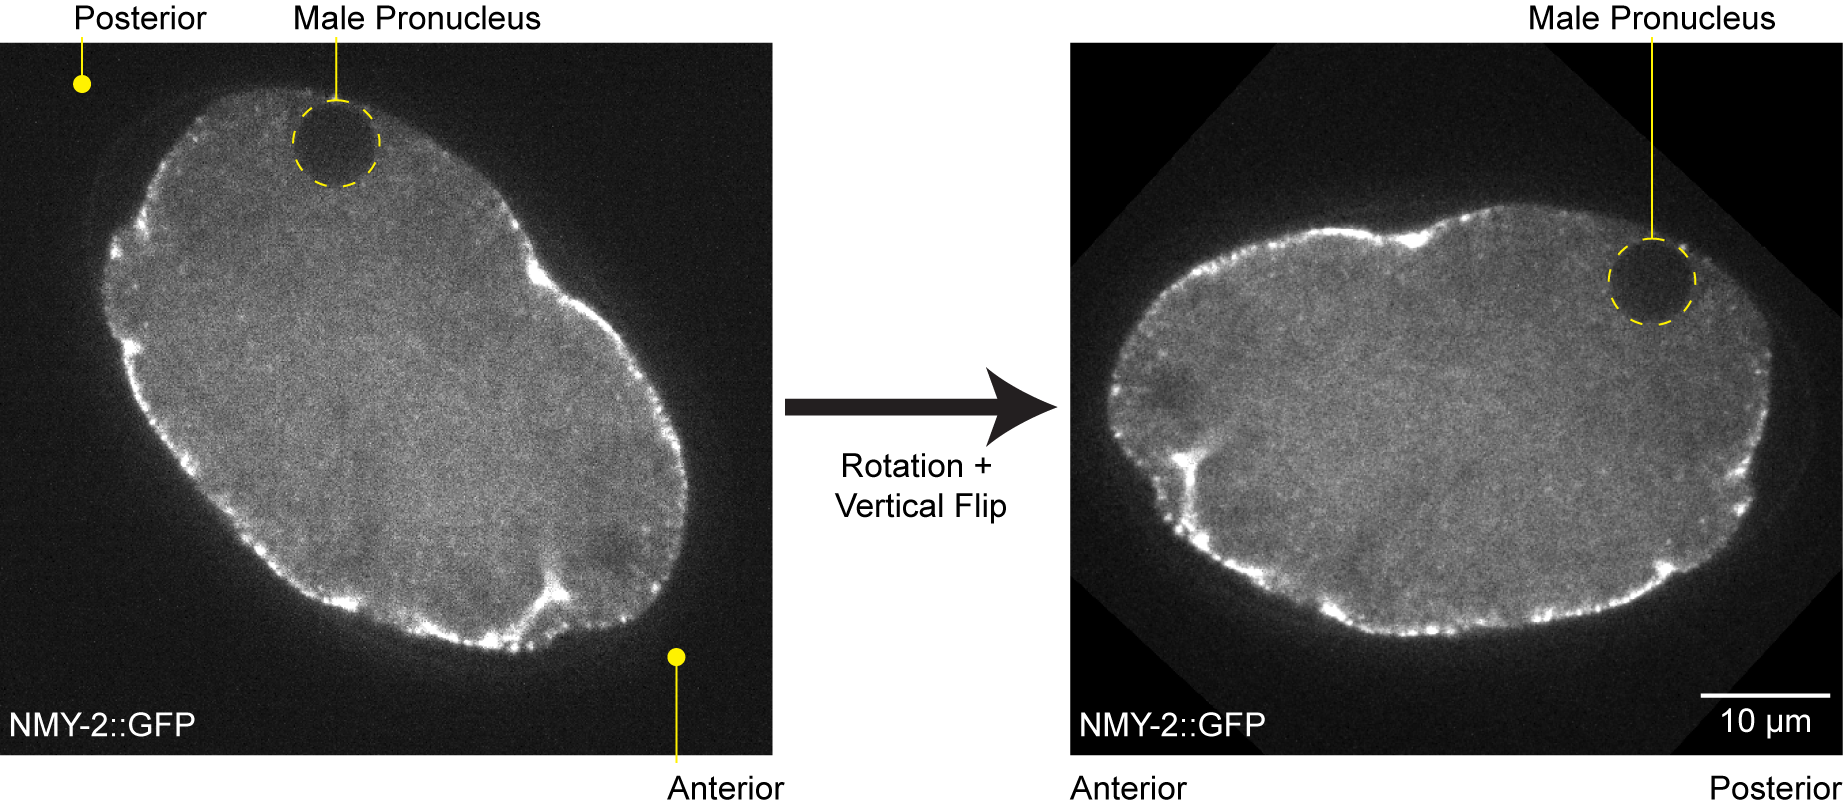
\includegraphics[width=0.9\textwidth]{ExpMethods/FigPreProcess/manualAnnotationRotation.png}   \caption{Left image (myosin channel) demonstrates the manual annotation done during pre-processing. Posterior end is recognized by the the presence of the male pronucleus (yellow dotted circle) and the associated depletion of myosin on the cortex. Two points are then marked to denote the posterior and anterior ends respectively (yellow dots near the ends of the embryo). Right image shows the result -- the image is rotated and then flipped (if necessary) to ensure that the anterior and posterior ends are on the left and right of the frame, and that the male pronucleus moves from the top of the embryo towards the posterior end. Scale bar: \SI{10}{\unitLength}} 
    \label{subfig:preprocess-manual}
\end{subfigure}
\hfill
\begin{subfigure}{\textwidth}
    \centering
    \includegraphics[width=\textwidth]{ExpMethods/FigPreProcess/selectNucleusRange.pdf}
    \caption{Myosin frames at different time-points depicting the movement of the male pronucleus (after rotation and flip). The frame where the male pronucleus first appears is denoted as the first frame. The frame where the male pronucleus starts moving away from the cortex -- and therefore the frame where posteriorisation ends -- is denoted as the last frame. Only the time-points that lie between the first and last frame are analysed (indicated by yellow dotted line). Time-points are denoted in \unit{\second}, with T = \SI{0}{\second} selected as the last frame, i.e. end of posteriorisation. Scale bar: \SI{10}{\unitLength}} 
    \label{subfig:preprocess-selectNucleusRange}
\end{subfigure}
\caption[Image analysis: pre-processing]{Pre-processing steps in the image analysis pipeline, for SWG070 strain. Anterior and posterior are to left and right respectively in all images.}
\label{fig:preprocess}
\end{figure}

For movies generated using SWG057 strain, step 1 of the pre-processing is modified --  see \autoref{fig:preprocessSWG057}. z-stack collected in the \ac{gfp} channel is used to detect the boundary of the embryo of interest in the frame. Kuwahara filter with window size \num{11} is used for noise reduction while still preserving edges \citep{kuwahara1976processing}. The z-stack is thresholded using the default thresholding method used by \ac{fiji} \citep{imageJGuide}. Maximum projection of this binary stack is then used to generate embryo boundary. If multiple embryos are present, only the binary mask corresponding to the embryo of interest is retained. The \ac{bf} images, \ac{nmy2} images and embryo outlines are arranged together in the same channel arrangement as those used for SWG070 movies. After this modification, movies from SWG057 strain are processed in the same as movies from the SWG070 strain.

\begin{figure}[p]
\centering
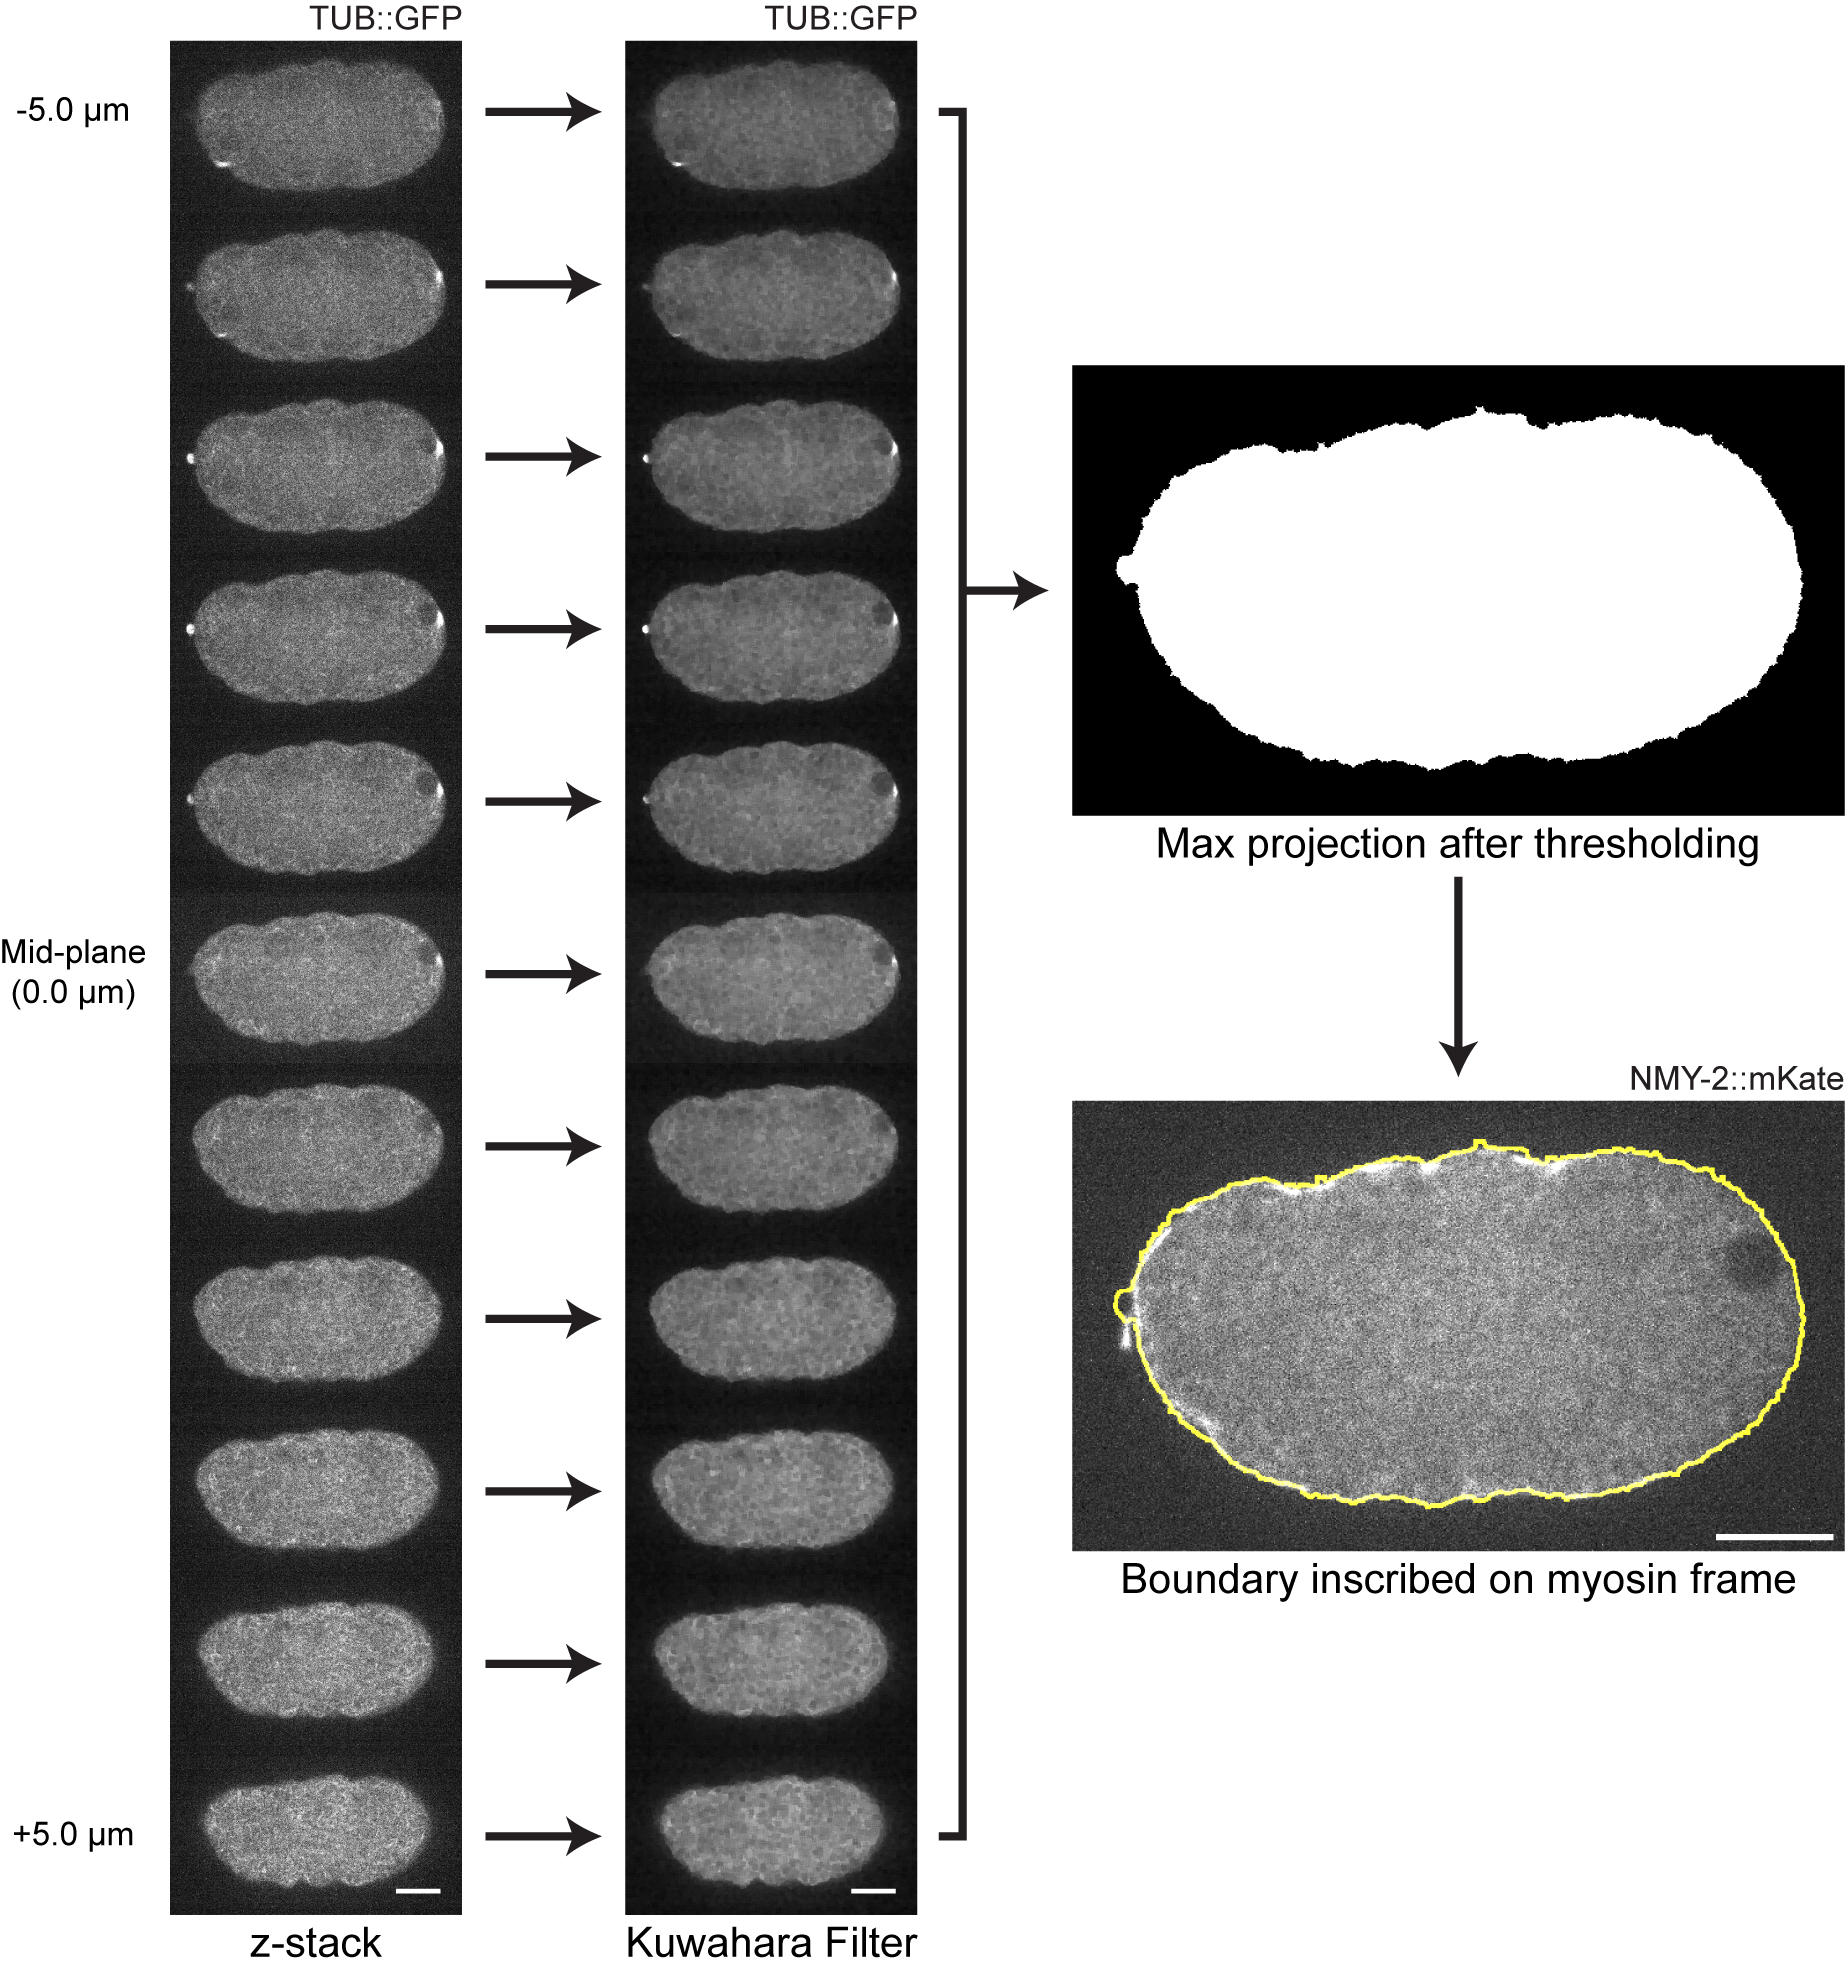
\includegraphics[width=\textwidth]{ExpMethods/FigPreProcess/swg057BoundaryDetect.png}
\caption[Image analysis: pre-processing (SWG057)]{Modified pre-processing steps for SWG057 strain, to extract embryo boundary from microtubule z-stacks. At each time-point, the z-stack of \num{11} slices in the microtubule channel are filtered using the kuwahara filter, binarized and then max projected. The outline of the max projection is encoded as the boundary channel, mimicking the \flurophoreLabel{phDomain}{mCherry} channel of the SWG070 strain. This outline is shown here as the yellow boundary inscribed onto the myosin frame at the same time-point. Scale bars in all images: \SI{10}{\unitLength}. Anterior and posterior are to left and right respectively in all images.}
\label{fig:preprocessSWG057}
\end{figure}

\subsection{Tracking posteriorisation of the male pronucleus}\label{subsec:nucleusTracking}
To track the position of the male pronucleus as it posteriorises, processed movies were analysed using a custom Python script. Following external packages were used in this Python script: openCV \citep{opencv}, tifffile \citep{tifffile}, scipy \citep{scipy} and numpy \citep{numpy}. This script expects the input movies to be a multipage tiff file with three channels -- first for \ac{bf} (which is not used in analysis), second for \ac{nmy2} and third denoting embryo boundary (example -- \flurophoreLabel{phDomain}{mCherry} in SWG070). These will be referred to as \ac{bf} channel, the myosin channel, and the boundary channel respectively.

\subsubsection{Segmenting the embryo boundary}\label{subsubsec:boundaryDetect}
For each time-point, the boundary channel frames are extracted and smoothed using a gaussian filter (with sigma = \SI{2}{\pixels}). Each frame are then thresholded using the 90th percentile of the intensity values in that frame as the threshold. A morphological closing operation (with disk element of size \SI{17}{\pixels}) is performed on the binary image thus constructed, to close any gaps in the boundary. To detect if the segmented embryo boundary is indeed closed, the inside of the boundary is filled using a binary fill holes operation. If the boundary is not filled, this operation will fill the whole frame instead. Thus, to detect if the boundary was closed, it is checked if more than \num{80}\% of the frame is filled. If less than \num{80}\% of the frame was filled, the boundary is closed -- extracted as the contour of non-zero length enclosing the largest area in the frame. If more than \num{80}\% of the frame was filled, a morphological dilation (with disk element of size \SI{18}{\pixels}) of the binary frame is performed to attempt closing gaps again. If after the dilation, binary fill holes still leads to more than \num{80}\% of the frame being filled, boundary detection is considered to have failed for this time-point and the boundary segmented in the previous time-point is used instead. Otherwise, the contour of non-zero length enclosing the largest area in the frame after dilation is again considered as the boundary. Boundary segmented at the previous time-point is also used if the boundary segmented at the current frame has a length too different from the previous one.

For each time-point, the segmented boundary is fit to an ellipse and the long and short axes of the fitted ellipse are calculated. To obtain the average axes for the movie, the axes detected for each time-point are averaged. The average direction is found by averaging the unit vectors that denote the instantaneous directions of the axes in each time-point, and the average lengths by averaging the lengths of the instantaneous axes. See \autoref{fig:segmentingEmbryoBoundary} for an example.

Additionally, the myosin channel frames are also denoised using non-local means denoising \citep{buades2011non}, with the following parameters: Filter strength = \SI{3}{\pixels}, template window size = \SI{4}{\pixels}, search window size = \SI{12}{\pixels}. 

\begin{figure}[H]
\centering
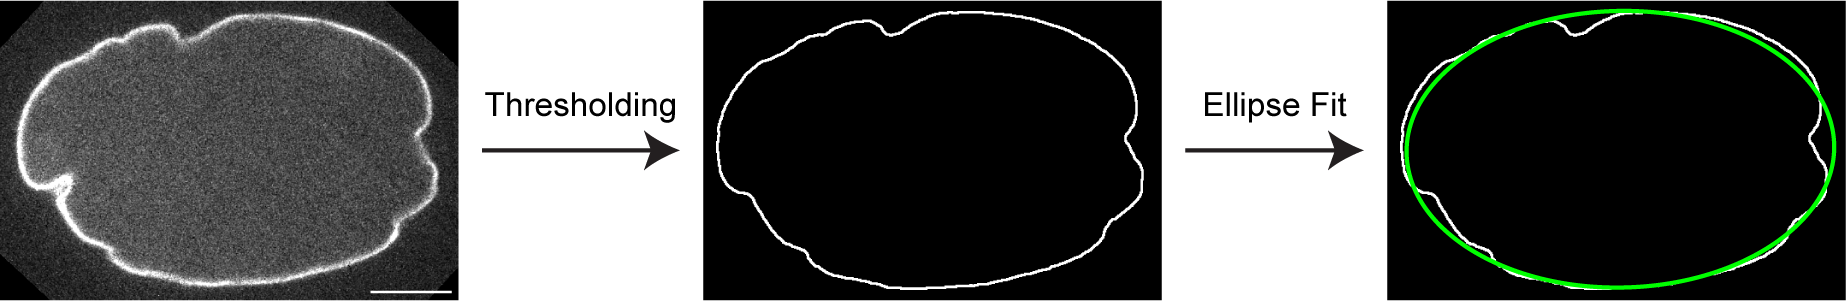
\includegraphics[width=\textwidth]{ExpMethods/FigTrackingPipeline/boundaryDetect.png}
\caption[Image analysis: Segmenting embryo boundary]{Boundary detection using the \flurophoreLabel{phDomain}{mCherry} channel in SWG070. At each time-point, the frame (left) is thresholded (middle, see \nameref{subsubsec:boundaryDetect} for details). The thresholded image provides the segmented boundary. An ellipse is fit to this segmented boundary to obtain the instantenous long and short axes (right, yellow line indicates the fitted ellipse). The same process is carried out on movies generated using embryos from the SWG057 strain. Scale bar: \SI{10}{\unitLength}}
\label{fig:segmentingEmbryoBoundary}
\end{figure}

\subsubsection{Segmenting the male pronucleus}\label{subsubsec:nucleusDetect}
The denoised myosin channel frames are utilized for segmenting the male pronucleus. Only myosin frames for the time-points in the range selected in \autoref{subsec:preprocess} are considered. In these frames, the pronuclei can be identified as dark circles devoid of myosin in the cytoplasm. The male pronucleus is identified as the one present in the posterior half (steps in \autoref{subsec:preprocess} ensure this is always true). This difference in intensities between the cytoplasmic myosin and male pronucleus is utilized to segment the latter, using successive thresholding. The following steps are undertaken for each myosin frame (that is, at each time-point) to segment the male pronucleus (see \autoref{fig:malePronucleusTrackingPipeline} for an example):
\begin{enumerate}
    \item The segmented embryo boundary is used to create a mask of the interior of the embryo -- in this way, the boundary segmentation is crucial for male pronucleus segmentation, as it allows separating the interior of the embryo from the whole frame.
    \item The set of thresholds to use for successive thresholding is selected, ranging from the \num{5}th to the \num{95}th percentile of the non-zero intensity values in the embryo interior.
    \item For each threshold in the selected range:
    \begin{enumerate}
        \item The frame is thresholded using the selected threshold. Pixels with intensity values below the selected threshold are set to be white (= \num{1}), and rest to black (= \num{0}).
        \item All pixels to the left (or in the anterior half) of the embryo center (determined as the center of the ellipse fit to the boundary) are set to black (= \num{0}). This ensures that only the male pronucleus is detected, which is present to the right (or in the posterior half). A morphological opening operation with disk element of size \SI{5}{\pixels} is performed to remove small regions of white pixels.
        \item The total number of white pixels for this threshold is recorded.
    \end{enumerate}
    \item To detect the thresholds to use for male pronucleus segmentation, the \enquote{knee} of the Number of white pixels vs Thresholds graph is detected. This \enquote{knee} indicates the threshold above which which the number of white pixels for each threshold increase rapidly, indicating that the white pixels are \enquote{flooding} outside the dark circle that denotes the male pronucleus. To detect this \enquote{knee}, at each threshold a cost function is calculated: the square root of the average of differences from the mean of the number of white pixels up until that threshold is calculated. The threshold for which this cost is the lowest is selected as the maximum threshold to be used for male pronucleus segmentation. See \autoref{subfig:malePronucleusTrackingPipeline-successiveThreshold} for an example.
    \item All thresholds upto this maximum threshold calculated in the last step are considered. The male pronucleus is identified as a dark circle. To quantify how circular a segmentation is, circularity measure\footnote{This measure is based on the isoperimeteric inequality: a geometric inequality that relates the surface area (perimeter for 2D) to the volume (area for 2D) of a region. In 2D, it states that the perimeter of any closed curve $L$ is related to the enclosed area $A$ as $L^2 >= 4\pi A$. Thus, in 2D, for all closed curves with the same perimeter, the one enclosing the most area is the circle.} $ = 4\pi\frac{\textrm{Area}}{\textrm{Perimeter}^2}$, where Area and Perimeter are of the segmented section, is used. Circularity is a dimensionless measure that ranges from \num{0} to \num{1}, with \num{1} being a perfect circle. From all segmentations generated by the thresholds considered in this step, the one that has the largest area and circularity is identified as the male pronucleus. See \autoref{subfig:malePronucleusTrackingPipeline-thresholdSelection} for an example.
\end{enumerate}

\begin{figure}[p]
\centering
\begin{subfigure}{\textwidth}
    \centering
    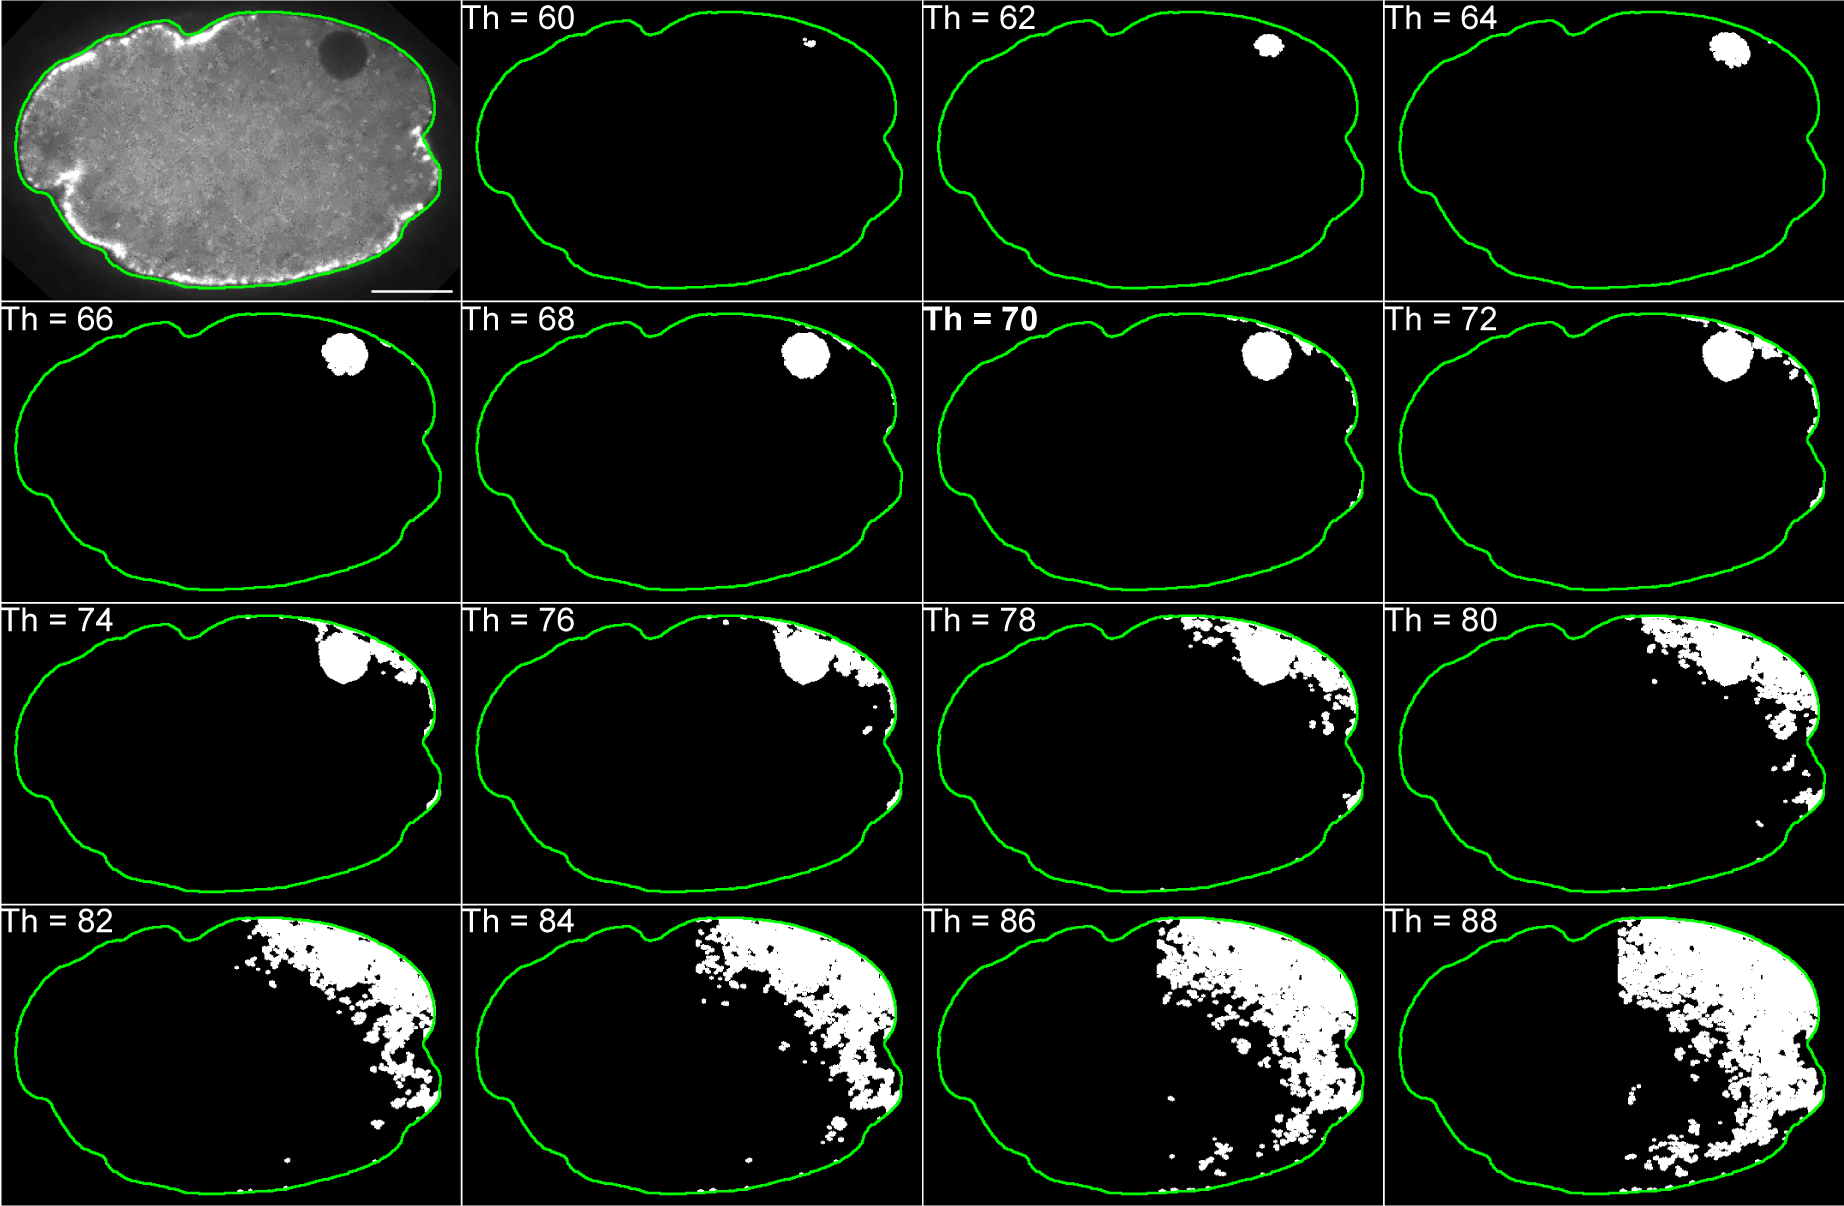
\includegraphics[width=0.9\textwidth]{ExpMethods/FigTrackingPipeline/successiveThreshold.png}
    \caption{Successive thresholding on myosin frame to segment male pronucleus. Top left image is the denoised myosin frame. All pixels outside this contour are ignored for the purposes of thresholding. Rest of the images show the result after thresholding at a specific threshold -- White pixels have intensities below the selected threshold. Yellow contour indicates the segmented boundary for all images. Note that any white pixels in the left half (that is, anterior half) of the embryo are automatically discarded. Threshold = \num{70} is selected for this myosin frame -- see \autoref{subfig:malePronucleusTrackingPipeline-thresholdSelection}. Scale bar: \SI{10}{\unitLength}} 
    \label{subfig:malePronucleusTrackingPipeline-successiveThreshold}
\end{subfigure}
\hfill
\vspace{1mm}
\begin{subfigure}{\textwidth}
    \centering
    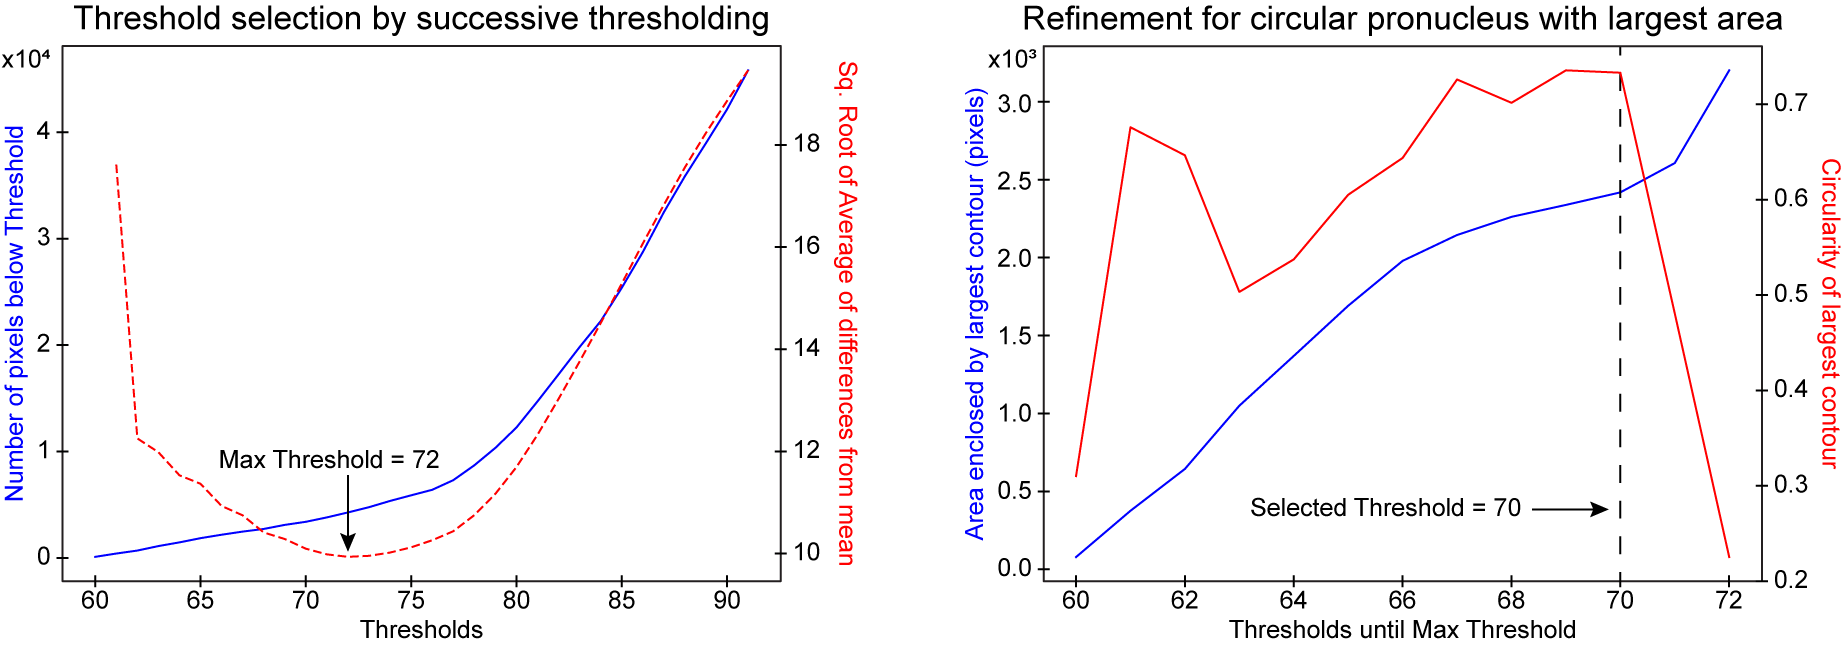
\includegraphics[width=\textwidth]{ExpMethods/FigTrackingPipeline/thresholdSelection.png}
    \caption{Automatic threshold selectiong using successive thresholding (see \nameref{subsubsec:nucleusDetect}). Left: Selecting Max Threshold. Blue curve (left y-axis) depicts the number of white pixels in the sense of \autoref{subfig:malePronucleusTrackingPipeline-successiveThreshold} for each threshold. Max Threshold is selected near the \enquote{knee} of this curve. Red dotted curve (right y-axis) depicts the cost function. Max Threshold is selected as the threshold with the minimum cost. Right: Selecting Threshold. All thresholds upto Max Threshold are considered. For each threshold, the area of the largest contour (that is, boundary of the largest connected component) is calculated (blue curve, left y-axis). Additionally, the circularity of this contour is calculated (red curve, right y-axis). Final selected threshold for this frame is where the area and circularity are both maximised. For this frame, the selected threshold is \num{70}. See \nameref{subsubsec:nucleusDetect} for definitions} 
    \label{subfig:malePronucleusTrackingPipeline-thresholdSelection}
\end{subfigure}
\caption[Image analysis: Segmenting the male pronucleus]{Segmenting the male pronucleus by successive thresholding and automatic selection. Only a single time-point is considered throughout the figure. Anterior and posterior are to left and right respectively in all images.}
\label{fig:malePronucleusTrackingPipeline}
\end{figure}

\subsubsection{Tracking the male pronucleus}\label{subsubsec:nucleusTrack}
Male pronucleus segmentations generated by the process outlined above are filtered to ensure the following:
\begin{itemize}
    \item The centers of consecutive male pronucleus segmentations (consecutive as in two consecutive time-points) do not have a distance exceeding \SI{13}{\pixels}. This ensures that spurious detections which are far from the male pronucleus are ignored. Given that the cortex and cytoplasm flow at speeds around \SIrange{0}{10}{\micro\meter\per\minute} (see \autoref{subsec:corticalFlows}) and the limitation here corresponds to a speed of \SI{27.3}{\micro\meter\per\minute} or more, no true segmentations are ignored.
    \item Segmentations which are too irregular -- that is, with circularity less than \num{0.7} --  are ignored.
    \item Segmentations which are very small -- that is, with area less than \SI{200}{\pixels^2} --  are ignored.
\end{itemize}
For frames where the segmentations are ignored, an estimate is generated by linearly interpolating between the two closest \enquote{good} frames, where the segmentations were not ignored. This is only done for gaps of \num{5} frames or less, and is not done at the edges of the set of frames selected for nucleus segmentation. The set of male pronucleus segmentations thus generated, as a function of time-points of each frame, constitute the detected trajectory of the male pronucleus in this movie.  

Both the male pronucleus trajectory and the embryo boundary detected using the above analyses are manually verified -- see \autoref{fig:validateSegmentations}. If a movie fails to detect any embryo boundary, or fails to detect the male pronucleus in more than \num{30}\% of frames selected, the movie is discarded.

Following attributes of the trajectory are calculated for each frame (see \autoref{fig:malePronucleusTrackingResults} and \autoref{fig:malePronucleusTrackingVelocities}):
\begin{description}
    \item[Pronucleus position]\hfill\\
    Calculated with respect to the embryo center, designated as origin. The x and y coordinates of the center of the pronucleus, and the polar angle between the long axis and the line connecting the center of the embryo to the center of the pronucleus are stored. This angle is referred to as the \enquote{Angular Position of the male pronucleus}.
    \item[Pronucleus Size]\hfill\\
    Calculated as the total number of pixels in the male pronucleus segmentation at each time-point.
    \item[Distance from cortex]\hfill\\
    Calculated as the distance between the center of the male pronucleus and the closest point on the embryo boundary (cortex).
    \item[Pronucleus velocity]\hfill\\
    Calculated as the gradient of the position of the male pronucleus. The component of the velocity along the x and y axes are stored. Additionally, components of the velocity parallel and perpendicular to the embryo boundary are also calculated. This component of the pronucleus velocity parallel to the embryo boundary is referred to as the \enquote{Posteriorisation velocity}.
\end{description}

\begin{figure}[p]
\centering
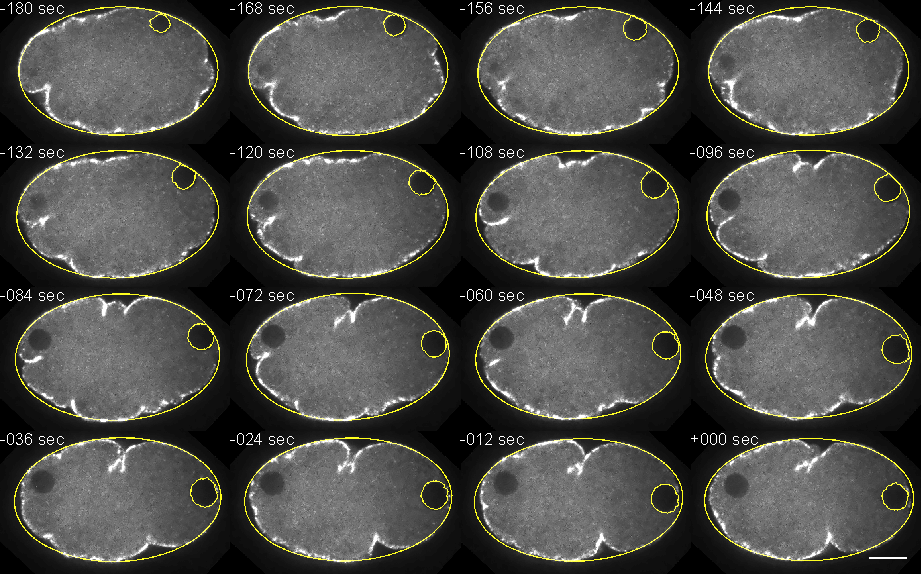
\includegraphics[width=\textwidth]{ExpMethods/FigTrackNucleus/validate.pdf}
\caption[Image analysis: Validation]{Validating the results of the segmentations, for different time-points. In each image, the outer yellow contour denotes the fitted ellipse to the segmented boundary, and the inner yellow contour denotes the segmented male pronucleus. Scale bar: \SI{10}{\unitLength}. Anterior is to the left and posterior to the right in all images. T = \SI{0}{\second} denotes end of posteriorisation.}
\label{fig:validateSegmentations}
\end{figure}

\begin{figure}[p]
\centering

\begin{subfigure}[t]{0.45\textwidth}
    \centering
    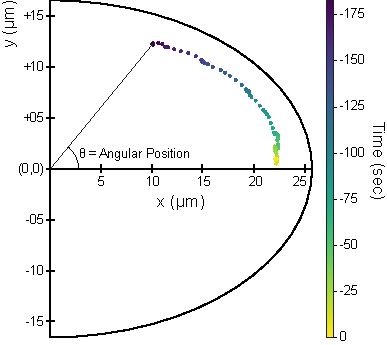
\includegraphics[width=\textwidth]{ExpMethods/FigTrackNucleus/trajectory.pdf}
    \caption{Trajectory of the male pronucleus -- denoted by the coordinates of its center -- as it posteriorises over time. Color represents time. x- and y-axes lie along the long and short axes of the ellipse fitted to the embryo boundary. Angular position is defined as the angle between the long axis and line connecting the centers of the male pronucleus and embryo.} 
    \label{subfig:malePronucleusTrackingResults-trackPronucleus}
\end{subfigure}
\hfill
\begin{subfigure}[t]{0.45\textwidth}
    \centering
    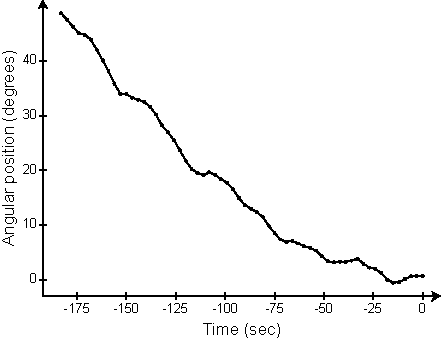
\includegraphics[width=\textwidth]{ExpMethods/FigTrackNucleus/angularPosVsTime.pdf}
    \caption{Plot of Angular position of the male pronucleus (y-axis) as a function of time (x-axis).} 
    \label{subfig:malePronucleusTrackingResults-angularPosVsTime}
\end{subfigure}

\begin{subfigure}[t]{0.45\textwidth}
    \centering
    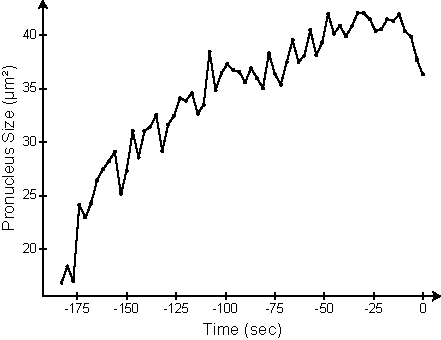
\includegraphics[width=\textwidth]{ExpMethods/FigTrackNucleus/sizeVsTime.pdf}
    \caption{Plot of the size of the male pronucleus (y-axis) as a function of time (x-axis). Size is measured as the area enclosed by the contour denoting the male pronucleus segmentation.} 
    \label{subfig:malePronucleusTrackingResults-sizeVsTime}
\end{subfigure}
\hfill
\begin{subfigure}[t]{0.45\textwidth}
    \centering
    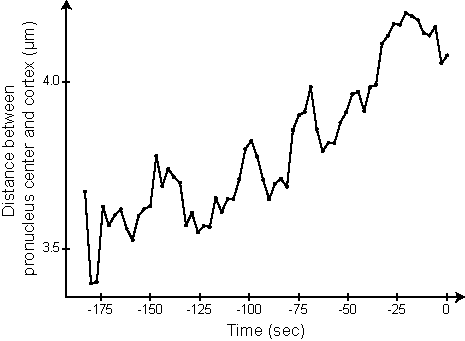
\includegraphics[width=\textwidth]{ExpMethods/FigTrackNucleus/crtxDistVsTime.pdf}
    \caption{Plot of Distance between the center of male pronucleus and closest point on cortex (y-axis) as a function of time (x-axis).} 
    \label{subfig:malePronucleusTrackingResults-crtxDistVsTime}
\end{subfigure}

\caption[Image analysis: Trajectory of male pronucleus]{Trajectory of the male pronucleus obtained using the image analysis pipeline. For all plots, T = \SI{0}{\second} denotes the end of posteriorisation. All plots are obtained from a single movie of an embryo of SWG070 strain -- same embryo depicted in \autoref{fig:imageAcquisition}, \autoref{fig:preprocess}, \autoref{fig:segmentingEmbryoBoundary}, \autoref{fig:malePronucleusTrackingPipeline} and \autoref{fig:validateSegmentations}}
\label{fig:malePronucleusTrackingResults}
\end{figure}

\begin{figure}[p]
\centering

\begin{subfigure}[t]{0.45\textwidth}
    \centering
    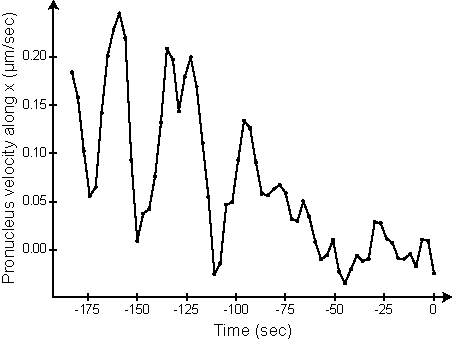
\includegraphics[width=\textwidth]{ExpMethods/FigTrackNucleus/vxVsTime.pdf}
    \caption{Plot of component of the velocity of the male pronucleus along the long axis (y-axis) as a function of time (x-axis). Positive velocity indicates movement towards posterior.} 
    \label{subfig:malePronucleusTrackingVelocities-vxVsTime}
\end{subfigure}
\hfill
\begin{subfigure}[t]{0.45\textwidth}
    \centering
    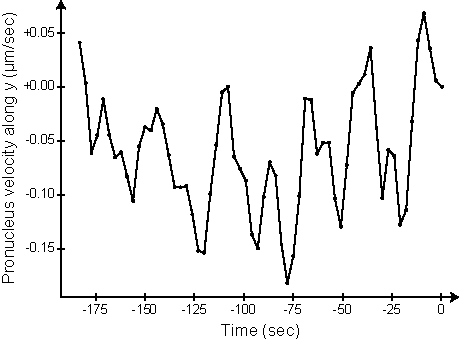
\includegraphics[width=\textwidth]{ExpMethods/FigTrackNucleus/vyVsTime.pdf}
    \caption{Plot of component of the velocity of the male pronucleus along the short axis (y-axis) as a function of time (x-axis). Positive velocity indicates movement towards the top of the embryo.} 
    \label{subfig:malePronucleusTrackingVelocities-vyVsTime}
\end{subfigure}

\begin{subfigure}[t]{0.45\textwidth}
    \centering
    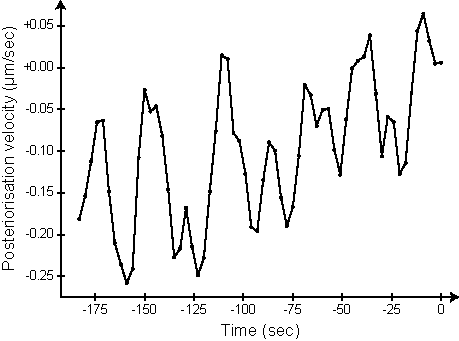
\includegraphics[width=\textwidth]{ExpMethods/FigTrackNucleus/postVelVsTime.pdf}
    \caption{Plot of the posteriorisation velocity of the male pronucleus (y-axis) as a function of time (x-axis). Posteriorisation velocity is defined as the component of the velocity of the male pronucleus parallel to the cortex. Positive velocity indicates movement towards posterior.} 
    \label{subfig:malePronucleusTrackingVelocities-postVelVsTime}
\end{subfigure}
\hfill
\begin{subfigure}[t]{0.45\textwidth}
    \centering
    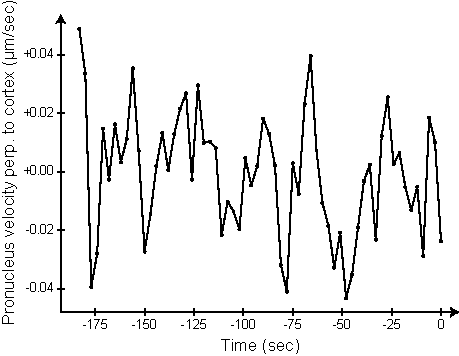
\includegraphics[width=\textwidth]{ExpMethods/FigTrackNucleus/perpVelVsTime.pdf}
    \caption{Plot of the component of the velocity of the male pronucleus perpendicular to the cortex (y-axis) as a function of time (x-axis). Positive velocity indicates movement towards the cortex.} 
    \label{subfig:malePronucleusTrackingVelocities-perpVelVsTime}
\end{subfigure}

\begin{subfigure}[t]{0.45\textwidth}
    \centering
    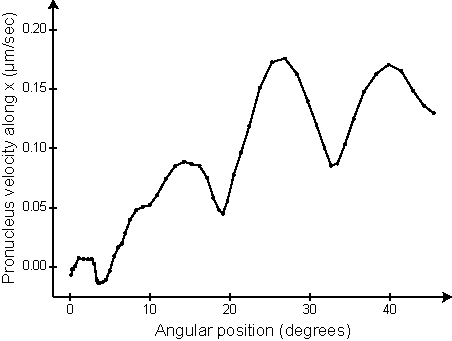
\includegraphics[width=\textwidth]{ExpMethods/FigTrackNucleus/vxVsAngleSmooth.pdf}
    \caption{Plot of component of the velocity of the male pronucleus along the long axis (y-axis) as a function of angular position (x-axis). Values have been smoothed using a sliding average with window of \num{7} frames. Positive velocity indicates movement towards posterior.} 
    \label{subfig:malePronucleusTrackingVelocities-vxVsAngleSmooth}
\end{subfigure}
\hfill
\begin{subfigure}[t]{0.45\textwidth}
    \centering
    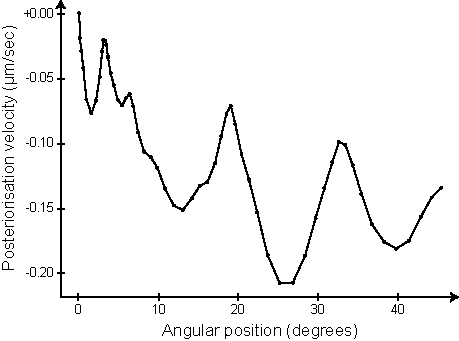
\includegraphics[width=\textwidth]{ExpMethods/FigTrackNucleus/postVelVsAngleSmooth.pdf}
    \caption{Plot of posteriorisation velocity of the male pronucleus (y-axis) as a function of angular position (x-axis). Values have been smoothed using a sliding average with window of \num{7} frames. Positive velocity indicates movement towards posterior.} 
    \label{subfig:malePronucleusTrackingVelocities-postVelVsAngleSmooth}
\end{subfigure}

\caption[Image analysis: Trajectory of male pronucleus (velocities)]{Velocities obtained using the image analysis pipeline. For plots against time, T = \SI{0}{\second} denotes the end of posteriorisation. All plots are obtained from a single movie of an embryo of SWG070 strain -- same embryo depicted in \autoref{fig:imageAcquisition}, \autoref{fig:preprocess}, \autoref{fig:segmentingEmbryoBoundary}, \autoref{fig:malePronucleusTrackingPipeline} and \autoref{fig:validateSegmentations}}
\label{fig:malePronucleusTrackingVelocities}
\end{figure}

\subsubsection{Measuring \ac{nmy2} concentrations}\label{subsubsec:myosinConc}
Myosin concentrations in the cytoplasm and cortex can be measured using the boundary segmentations and denoised myosin frames obtained from the Python script. Myosin concentration are measured in intensity per pixel units, where intensity is measured in arbitrary units corresponding to the readings from the camera used to record the movies. A region \SI{15}{pixels} wide below the segmented boundary is considered as being at the cortex, while the cytoplasm is considered as the interior region, left after the cortical region is removed. Myosin concentration in each region is estimated as the average intensity per pixel in the corresponding region, averaged over \num{7} consecutive frames (sliding window).

\subsection{Measuring cortical flows}\label{subsec:corticalFlows}
Cortical flows were measured from the denoised myosin frames using a custom \ac{matlab} script, following \cite{gross2019guiding} (\ac{matlab} script written by Peter Gro{\ss}). The script takes as input the boundary segmentations and the denoised myosin frames generated by the Python script, and performs two steps:
\begin{enumerate}
    \item Using the boundary segmentations already made by the Python script, the \ac{matlab} script generates a kymograph of the cortical layer in the myosin frames. The cortical layer is identified as the region starting from the boundary of the embryo and stretching \SI{30}{\pixels} deep inwards.
    \item These kymographs are then used to measure the flow velocity of the cortex as a function of position along the cortex, using \ac{piv} \citep{thielicke2014pivlab}.
\end{enumerate}
See \autoref{fig:crtxFlowMeasurement} for output kymographs and cortical flows, for the example movie considered in this chapter.

\subsubsection{Creating kymographs}\label{subsubsec:kymographs}
For a given myosin frame, its corresponding boundary segmentation (generated by the Python script) is converted into a composite B{\'e}zier curve: a series of B{\'e}zier curves joined end to end. This converts the discrete pixel positions of the boundary segmentation into a smooth curve that represents the embryo boundary. The point on this curve that is on the embryo's long axis and at the posterior end are identified. Starting from this point, additional points are sampled at one pixel size distance between adjacent points on both ends of the curve. Denoting the initial point on the posterior as zero, these points denote the integer distances along the curve, that is integer arclengths. Thus, the composite B{\'e}zier curve is used to define the distance along the cortex -- the arclength axis. 

At each point sampled on the curve, the normal to the curve pointing towards the embryo interior is found. Points are sampled along each normal at one pixel size distance between adjacent points on a normal upto a distance of \SI{30}{\pixels}, and pixel values are interpolated to obtain the estimated intensities at these points. This can be folded out into a thin rectangular \enquote{band}\footnote{The change in length between the outermost points at the boundary and innermost points towards the embryo interior are ignored, as the length of the embryo boundary is much larger than \SI{30}{\pixels}} of points along the embryo boundary. This \enquote{band} is identified as a folded out version of the cortex, calculating for the frame of interest. The long edge of this band is along the arclength axis, while the short edge is perpendicular. 

By taking the maximum intensity value along this perpendicular axis for each point on the arclength axis (maximum projection), and stacking the resultant 1D representations of myosin distributions for each frame in order of time vertically, a visualization known as the kymograph can be generated -- see \autoref{subfig:crtxFlowMeasurement-kymographFullMovie} and \autoref{subfig:crtxFlowMeasurement-kymographPosteriorization}. This kymograph allows visualization of the changes in myosin distributions as a function of time at each position on the cortex.

\subsubsection{\acf{piv}}\label{subsubsec:pivCortex}
\ac{piv} is a method of visualizing flow in fluids and measuring instantaneous flow velocities \citep{raffel1998particle,thielicke2014pivlab}. Under this method, the fluid is seeded with tracer particles which can be illuminated with light. These tracer particles are small enough that they can be assumed to faithfully follow the fluid dynamics. Time-lapse movies of the fluid flow, with the tracer particles illuminated, are taken. Instead of tracking individual particles, the flow field at a given time-point is calculated by cross-correlating sections of the frame at this time-point with the frame at the next section. In detail, the frame at the current time-point is divided into templates of defined sizes. Each template is cross-correlated with the frame at the next time-point by displacing the template upto a maximum distance from its location in the current time-point. Displacement with the largest cross-correlation, divided by the time elapsed between the two frames, is the measured velocity of the fluid at the location of the template. Here a multi-pass \ac{piv} algorithm is used, which uses templates of different sizes to measure fluid flow at finer resolutions; along with Gaussian fitting of the peak in the cross-correlation to obtain subpixel accuracy. See \cite{raffel1998particle} for a detailed discussion. 

In the case of the cortex, since myosin motors are fluorescently labelled, tracer particles are not required -- fluorescent tags take the role of the tracer particles. To calculate cortical flow velocities along the arclength axis, the cortical \enquote{bands} extracted for each frame are used for the cross-correlations instead. A multi-pass (4 passes) PIV was utilized, with initial template size of \SI{24}{\pixels} and step size of \SI{4}{\pixels}. Max displacement of each template during cross-correlation was limited to \SI{7}{\pixels}. See \autoref{subfig:crtxFlowMeasurement-crtxFlows} for the measured cortical flows in the example movie considered for this chapter.

\begin{figure}[p]
\centering

\begin{subfigure}[t]{0.45\textwidth}
    \centering
    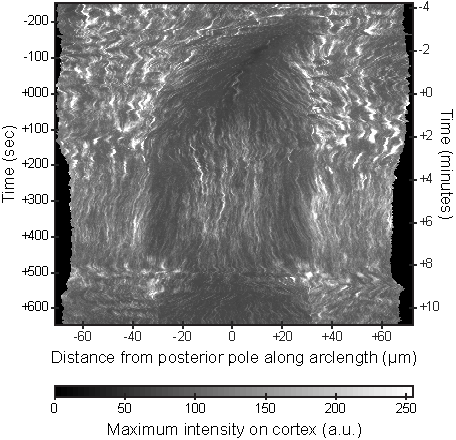
\includegraphics[width=\textwidth]{ExpMethods/FigCrtxFlows/kymographFullMovie.pdf}
    \caption{Kymograph depicting intensities along the cortex (arclength axis along x-axis) as a function of time (along y-axis), for the full movie. Colorbar indicates the maximum intensity value on the cortex at the given position and time.} 
    \label{subfig:crtxFlowMeasurement-kymographFullMovie}
\end{subfigure}
\hfill
\begin{subfigure}[t]{0.45\textwidth}
    \centering
    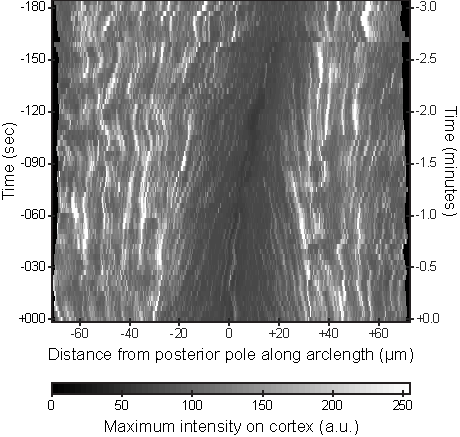
\includegraphics[width=\textwidth]{ExpMethods/FigCrtxFlows/kymographPosteriorization.pdf}
    \caption{Kymograph depicting intensities along the cortex (arclength axis along x-axis) as a function of time (along y-axis), only for time-points used to analyze posteriorisation. Colorbar indicates the maximum intensity value on the cortex at the given position and time.} 
    \label{subfig:crtxFlowMeasurement-kymographPosteriorization}
\end{subfigure}

\begin{subfigure}{\textwidth}
    \centering
    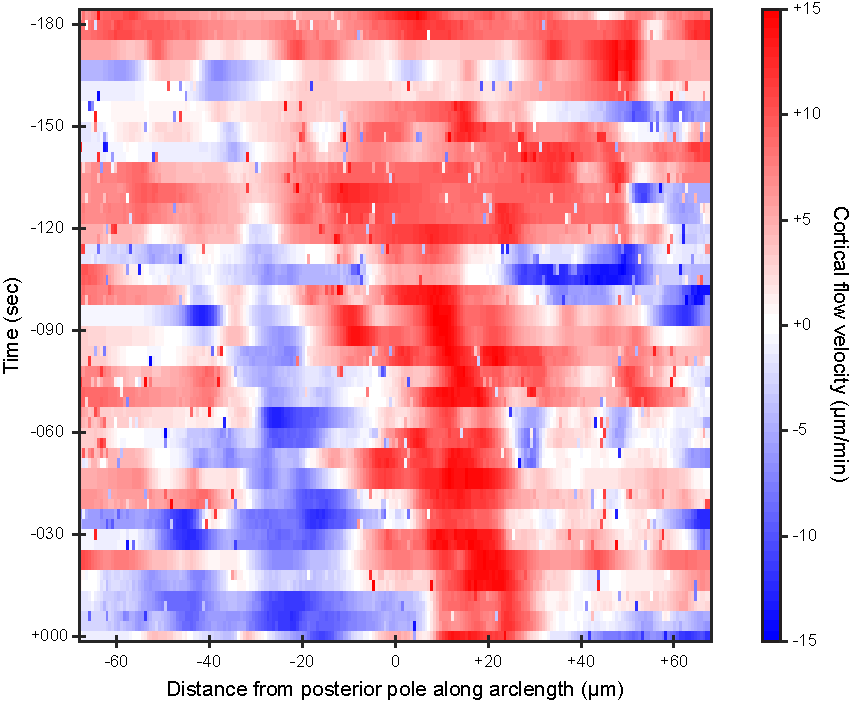
\includegraphics[width=0.8\textwidth]{ExpMethods/FigCrtxFlows/crtxFlows.pdf}
    \caption{Cortical flow velocity (colorbar) measured for the time-points used to analyse posteriorization, as a function of time (y-axis) and position along the cortex (x-axis). Positive/Negative flow velocity, depicted in red/blue, indicate movement towards/away from positive end of the arclength axis (x-axis).} 
    \label{subfig:crtxFlowMeasurement-crtxFlows}
\end{subfigure}

\caption[Image analysis: Measuring cortical flows]{Measuring cortical flows. For all plots, T = \SI{0}{\second} on the y-axis denotes the end of posteriorisation, and s = \SI{0}{\unitLength} on the x-axis denotes the posterior pole. All plots are obtained from a single movie of an embryo of SWG070 strain -- same embryo depicted in \autoref{fig:imageAcquisition}, \autoref{fig:preprocess}, \autoref{fig:segmentingEmbryoBoundary}, \autoref{fig:malePronucleusTrackingPipeline} and \autoref{fig:validateSegmentations}}
\label{fig:crtxFlowMeasurement}
\end{figure}

\subsection{Measuring cytoplasmic flows}\label{subsec:cytoFlows} %%TODO: CHECK PARAMETERS
Cytoplasmic flows in the embryos were measured using the \ac{bf} frames in the embryo movies (see \autoref{sec:imageAnalysis}). A MATLAB implementation of \ac{piv} \citep{thielicke2014pivlab} was used to calculate the flow fields in the cytoplasm from the \ac{bf} frames (see \autoref{subsec:corticalFlows} for general introduction to \ac{piv}), with the boundary segmentations (see \autoref{subsec:nucleusTracking}) used to exclude the exterior of the embryo. Yolk granules in the cytoplasm serve the role of the tracer particles in the cytoplasm. A multi-pass (4 passes) PIV was utilized, with initial template size of \SI{24}{\pixels} and step size of \SI{4}{\pixels}. Max displacement of each template during cross-correlation was limited to \SI{7}{\pixels}. 

\section{Data analysis}\label{sec:statAnalysis}
This section describes the methods used to analyse the data -- male pronucleus trajectories and cortical flows measured for each embryo -- to obtain ensemble averages for a given experiment. Average posteriorisation velocity as a function of angular position of the male pronucleus is used as the primary measure of \ac{ap} axis alignment. Average cortical flows as a function of angular position of the male pronucleus are used as the input for the calibration process described in \autoref{ch:ActiveMatter}. For all experimental conditions, the average posteriorisation velocity and average cortical flows as a function of angular position are calculated. All data analysis is done using custom scripts written in \ac{matlab}.

Short-term fluctuations in each male pronucleus trajectory are smoothed using a sliding average with a window of \SI{7}{\frames} for each movie separately. To calculate average posteriorization velocity as a function of angular position, posteriorization velocity and angular positions calculated for all embryos for a given experimental condition are combined together. Angular positions in this dataset are binned in \SI{3}{\unitAngle} bins. Average posteriorization velocity for each angular position bin is calculated by averaging over all posteriorization velocities corresponding to the angular positions included in the bin. \num{95}\% confidence interval for the mean posteriorization velocities are calculated using a two-sided t-test. See \autoref{subfig:dataAnalysisExample-postVel} for an example.

Cortical flows measured for all embryos for a given experimental condition are first aligned using the arclength axis. Cortical flows are then classified using the angular position of the male pronucleus, and binned together in angular position bins of \SI{3}{\unitAngle} width each. Average cortical flows for each angular position bin are calculated by averaging all cortical flows within an angular position bin. Note that this averaging is done spatially: that is, measured flow velocities at the same position on the arclength axis corresponding to different frames are averaged together. The model described in \autoref{ch:ActiveMatter} uses these averaged cortical flows for calibration. See \autoref{subfig:dataAnalysisExample-crtxFlow} for an example.

\begin{figure}[h]
\centering
\begin{subfigure}[t]{0.45\textwidth}
    \centering
    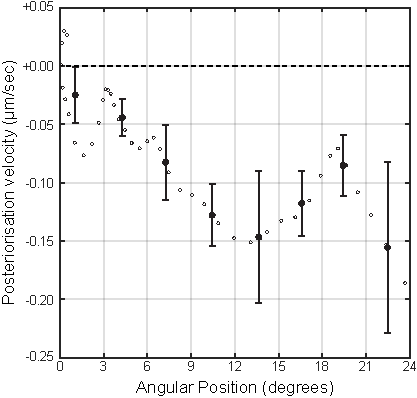
\includegraphics[width=\textwidth]{ExpMethods/FigDataAnalysis/postVel.pdf}
    \caption{Binning Posteriorization velocity (y-axis) vs Angular position (x-axis). Each angular position bin is of \SI{3}{\unitAngle} width. For each bin, the mean posteriorization velocity (dark circles) and 95\% confidence intervals of the mean (error bars) are depicted. Open circles denote the datapoints obtained after smoothing via sliding average (window: \num{7} frames). Dotted line indicates zero posteriorization velocity.} 
    \label{subfig:dataAnalysisExample-postVel}
\end{subfigure}
\hfill
\begin{subfigure}[t]{0.5\textwidth}
    \centering
    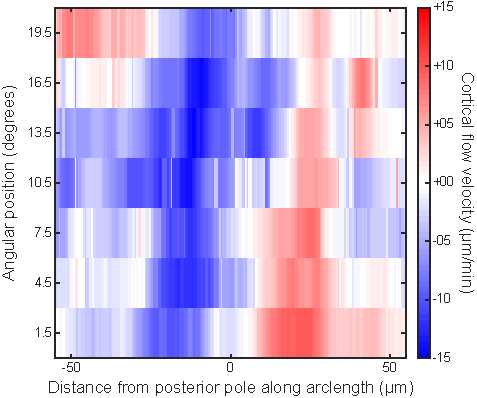
\includegraphics[width=\textwidth]{ExpMethods/FigDataAnalysis/crtxFlow.pdf}
    \caption{Binning Cortical flow velocity (colorbar) using Angular position (y-axis). For each angular position bin (bin width \SI{3}{\unitAngle}), the mean cortical flow at each position along the cortex (x-axis) is calculated -- using all frames that fall within the angular position bin. Positive/Negative flow velocity, depicted in red/blue, indicate movement towards/away from positive end of the arclength axis (x-axis). s = \SI{0}{\unitLength} on the x-axis denotes the posterior pole.} 
    \label{subfig:dataAnalysisExample-crtxFlow}
\end{subfigure}
\caption[Data Analysis (example movie only)]{Data analysis done for a single movie of an embryo of SWG070 strain, for illustrative purpose. Movie depicted in \autoref{fig:imageAcquisition}, \autoref{fig:preprocess}, \autoref{fig:segmentingEmbryoBoundary}, \autoref{fig:malePronucleusTrackingPipeline} and \autoref{fig:validateSegmentations}. This figure showcases the two main output graphs obtained from the data analysis.}
\label{fig:dataAnalysisExample}
\end{figure}

\chapter{Experimental investigation of \acs{ap} axis alignment}\label{ch:Results}
In this chapter, the results of various experiments conducted to investigate \ac{ap} axis alignment in \ac{ce} embryo are reported, along with their comparison to the numerical simulations of the theoretical model of \ac{ap} axis alignment described in \autoref{sec:apAxisAlignmentModelMN}. This chapter follows \citep{axisConvergence} closely. Experiments described here were performed in collaboration with Peter Gross and Mirna Kramer from Technische Universit{\"a}t Dresden; with numerical simulations by Michael Nestler from Technische Universit{\"a}t Dresden.

\begin{table}
    \centering
    \begin{tabular}{|C{0.3\textwidth}|C{0.3\textwidth}|C{0.3\textwidth}|}
        \hline
        Experimental Condition & Strain & No. of Embryos\\
        \hline
        Unperturbed & SWG070 & \num{57}\\
        \geneExp{mlc-4} \ac{rnai} & SWG070 & \num{10}\\
        \geneExp{nop-1} \ac{rnai} & SWG070 & \num{9}\\
        \geneExp{nop-1; mel-11} \ac{rnai} & SWG070 & \num{69}\\
        \geneExp{ima-3} \ac{rnai} & SWG070 & \num{35}\\
        \geneExp{air-1} \ac{rnai} & SWG070 & \num{23}\\
        \geneExp{air-1; mel-11} \ac{rnai} & SWG228 & \num{13}\\
        Unperturbed & SWG057 & \num{32}\\
        \geneExp{goa-1; gpa-16} \ac{rnai} & SWG057 & \num{30}\\
        \hline
    \end{tabular}
    \caption{Number of embryos in various experimental conditions described in this chapter.}
    \label{tab:resultsNumberEmbryo}
\end{table}

\section{Characterising \acs{ap} axis alignment in unperturbed embryos} \label{sec:apAxisAlignCharacteriseWT}
\ac{ap} axis alignment is first characterised in unperturbed embryos. \enquote{Unperturbed} here refers to no genetic perturbations, such as no \ac{rnai} or mutations, apart from the addition of fluorescent tags. To this end, time-lapse microscopy of embryos from the SWG070 strain was undertaken, which is labelled with \flurophoreLabel{\ac{nmy2}}{\ac{gfp}} and \flurophoreLabel{phDomain}{mCherry} -- as described in \autoref{sec:microscope}. In these embryos, the male pronucleus can be observed as a dark circle in the cytoplasm, in the \flurophoreLabel{\ac{nmy2}}{\ac{gfp}} fluorescent channel -- as cytoplasmic myosin is excluded from the proncleus. The posterior domain as the depletion of \ac{nmy2} on the cortex near the male pronucleus. The \ac{ap} axis alignment process is characterised by tracking the position of the male pronucleus as it undergoes posteriorisation. See \autoref{sec:imageAnalysis} for details on the image analysis methods used to track the male pronucleus. 

\begin{figure}
\centering
\includegraphics[width=\textwidth]{Results/FigExpUnperturbed/wtMicrograph.pdf}
\caption[Representative micrograph: Unperturbed embryos]{Representative unperturbed embryo of SWG070 strain, labelled with \flurophoreLabel{\ac{nmy2}}{\ac{gfp}} (white), showing the posteriorisation of the male pronucleus and the concurrent movement of the myosin depletion (indicating the \ac{ppar} domain) towards the posterior end. The male pronucleus can be visualized as the dark circle in the myosin channel towards the posterior end (right). t = \SI{0}{\second} is set at the end of posteriorisation of the male pronucleus. Scale bar: \SI{10}{\unitLength}. Images are rotated such that anterior and posterior ends are to the left and right respectively.}
\label{fig:swg070WtMicrograph}
\end{figure}

Two aspects of the posteriorisation of the male pronucleus are quantified: its \enquote{angular position} and \enquote{posteriorisation velocity} (see \autoref{sec:imageAnalysis}). Angular position refers to the angle made between the long axis and the line connecting the center of the male pronucleus to the center of the embryo. Posteriorisation velocity is the component of the velocity of the male pronucleus that is parallel to the cortex (at the given angular position). Negative posteriorisation velocities indicate movement in direction of decreasing angular positions and thus towards the posterior end, positive posteriorisation velocity in direction of increasing angular positions and thus away from the posterior end. End of posteriorisation is denoted as the zero time-point (t = \SI{0}{\second}), and all movies are synchronised using this time-point. 

Plotting the angular position as a function of time, the angular positions were found to generally decrease towards \SI{0}{\unitAngle} as time reaches closer to end of posteriorisation (t = \SI{0}{\second}). Specifically, in embryos where the \ac{ap} axis is mis-aligned -- that is, with initial angular position greater than \SI{5}{\unitAngle} (\num{33} out of \num{57} embryos) -- the \ac{ap} axis re-aligns back towards the long axis. Furthermore, this decay towards \SI{0}{\unitAngle} was quantified by fitting an exponential $\alpha = \alpha_0 + \exp(-\frac{t}{t_0})$ to the plotted angular positions, yielding a time constant $t_0 = \SI{119 +- 3}{\second}$ and $\alpha_0 = \SI{-0.75 +- 0.3}{\unitAngle}$. These observations confirm those made in \cite{goldstein1996specification} -- the \ac{ap} axis does align itself towards the long axis of the embryo, evidenced by the posteriorisation of the male pronucleus. Note that the exponential fit considered here is only phenomenological, and does not attempt to capture any physically relevant features of \ac{ap} axis alignment -- rather it allows for easier comparison of the decreasing angular positions in different experimental conditions considered in this chapter.

\begin{figure}
\centering
\begin{subfigure}[t]{0.4\textwidth}
    \centering
    \includegraphics[width=\textwidth]{Results/FigExpUnperturbed/wtTrajectories.pdf}
    \caption{Trajectories of the male pronucleus (denoted by the coordinates of its center) observed in unperturbed embryos. Color represents time. x- and y-axes lie along the long and short axes of an ellipse with semi-major axis $a = \SI{28.9}{\unitLength}$ and semi-minor axis $b = \SI{16.3}{\unitLength}$. Scale bar: \SI{5}{\unitLength}} 
    \label{subfig:swg070WtTrajectories-tracks}
\end{subfigure}
\hfill
\begin{subfigure}[t]{0.57\textwidth}
    \centering
    \includegraphics[width=\textwidth]{Results/FigExpUnperturbed/wtAngular.pdf}
    \caption{Angular position of the male pronucleus (on y-axis, in \si{\unitAngle}) plotted as a function of time (on x-axis, in \si{\second}), in unperturbed embryos. Thin grey lines represent individual trajectories, thick black line represents a exponential fit to the average of these tracks: $\alpha = \alpha_0 + \exp(-\frac{t}{t_0})$, with $t_0 = \SI{119 +- 3}{\second}$ and $\alpha_0 = \SI{-0.75 +- 0.3}{\unitAngle}$.} 
    \label{subfig:swg070WtTrajectories-angleVsTime}
\end{subfigure}
\caption[Experimentally observed trajectories of the male pronucleus in unperturbed embryos]{Experimentally observed trajectories of the male pronucleus during posteriorisation in unperturbed embryos of SWG070 strain (N = 57). See \autoref{subsec:nucleusTracking} for details on male pronucleus tracking. Average semi-major and semi-minor axes lengths for unperturbed embryos of SWG070 strain are used in \autoref{subfig:swg070WtTrajectories-tracks} -- see \autoref{tab:resultsEmbryoGeometry}. Angular position is defined as the angle between the long axis and line connecting the centers of the male pronucleus and embryo, depicted in \autoref{subfig:swg070WtTrajectories-tracks}. t = \SI{0}{\second} denotes end of posteriorisation.}
\label{fig:swg070WtTrajectories}
\end{figure}

Plotting the posteriorisation velocity as a function of angular position (see \autoref{sec:statAnalysis} for details on binning of angular positions), it is found that the male pronucleus is, on average, moving towards the posterior end (as indicated by the negative sign of the velocity) -- with higher speed at higher angular positions (\autoref{fig:swg070WtPostVelVsAngle}). This can also be observed as increasing magnitude of slope of the angular position vs time plots for higher angular positions in \autoref{subfig:swg070WtTrajectories-angleVsTime}. Based on this observation, it is concluded here that the rate of \ac{ap} axis alignment is faster at higher angular positions: the male pronucleus moves faster towards the posterior end the further away from the posterior end it is.

\begin{table}
    \centering
    \begin{tabular}{|C{0.2\textwidth}|C{0.55\textwidth}|C{0.2\textwidth}|}
        \hline
        Angular positions (\si{\unitAngle}) & Posteriorisation velocity (\SI{1e-1}{\unitPostVel}) & No. of embryos\\
        \hline
        \numrange{0}{3} & \num{-0.15} (\num{-0.18},\num{-0.13}) & 37\\
        \numrange{3}{6} & \num{-0.17} (\num{-0.20},\num{-0.14}) & 36\\
        \numrange{6}{9} & \num{-0.27} (\num{-0.30},\num{-0.23}) & 31\\
        \numrange{9}{12} & \num{-0.40} (\num{-0.46},\num{-0.35}) & 27\\
        \numrange{12}{15} & \num{-0.46} (\num{-0.52},\num{-0.41}) & 20\\
        \numrange{15}{18} & \num{-0.40} (\num{-0.47},\num{-0.34}) & 16\\
        \numrange{18}{21} & \num{-0.49} (\num{-0.58},\num{-0.40}) & 13\\
        \numrange{21}{24} & \num{-0.85} (\num{-0.98},\num{-0.72}) & 10\\
        \numrange{24}{27} & \num{-1.12} (\num{-1.26},\num{-0.97}) & 8\\
        \hline
    \end{tabular}
    \caption{Posteriorisation velocity measured for each angular position bin in unperturbed embryos. Average posteriorisation velocity along with \num{95}\% confidence interval for the average are reported.}
    \label{tab:resultsPostVelUnperturbed}
\end{table}

\begin{figure}[p]
\centering
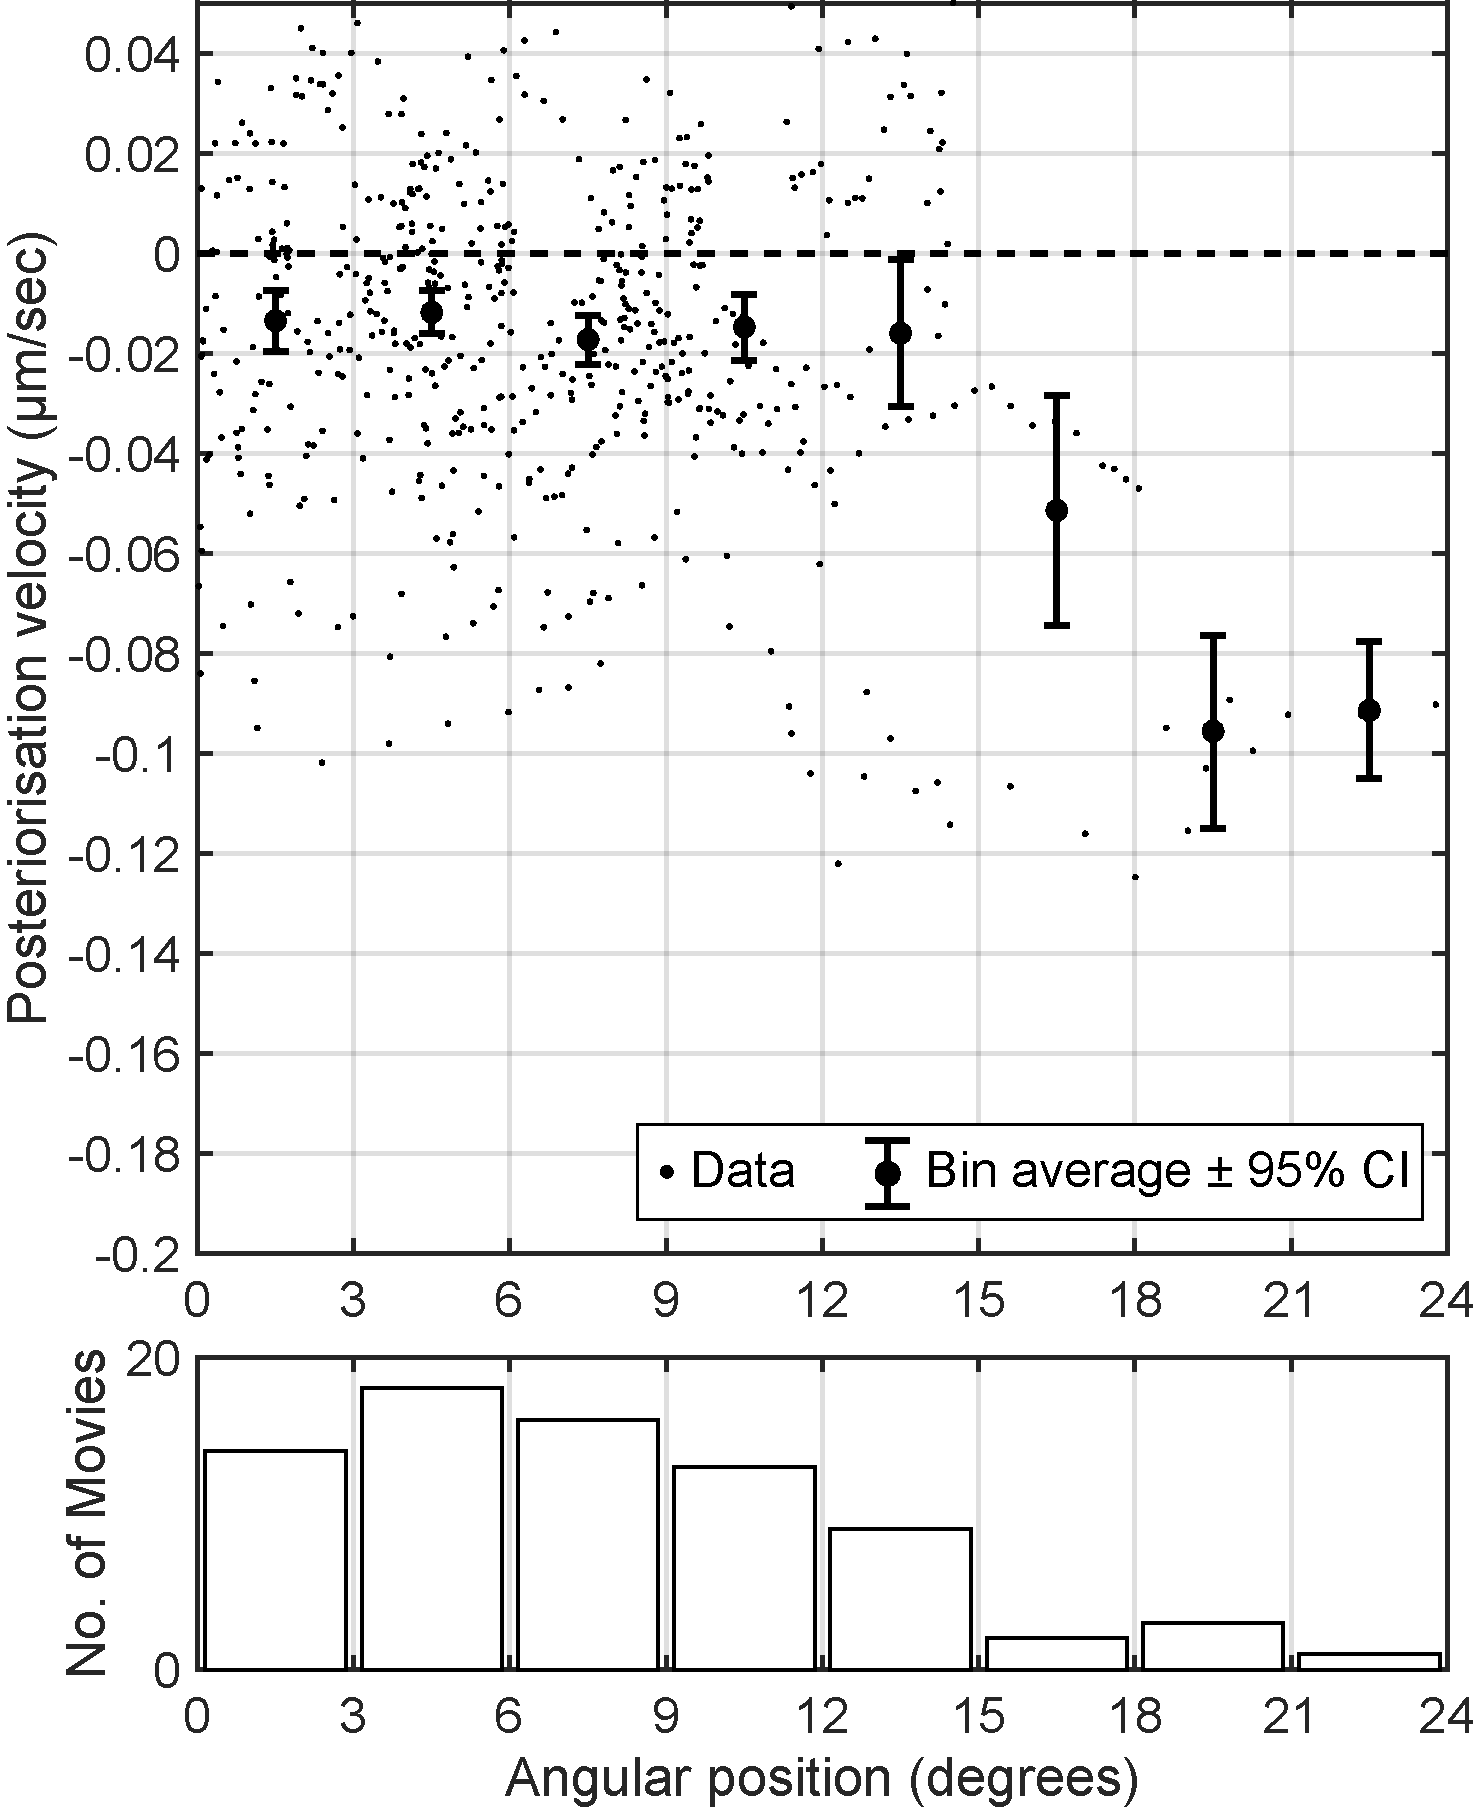
\includegraphics[width=0.95\textwidth]{Results/FigExpUnperturbed/wtPostVel.pdf}
\caption[Experimentally observed posteriorisation velocity of the male pronucleus in unperturbed embryos]{Top: Posteriorization velocity of the male pronucleus (along y-axis, in \si{\unitPostVel}) plotted against its angular position, in unperturbed embryos of SWG070 strain (N = 57). Negative values of the posteriorisation velocity indicate movement towards the posterior end. Angular position is binned using a bin width of \SI{3}{\unitAngle}. Black circles with errors bars denote the average posteriorization velocity with \num{95}\% confidence intervals in each angular position bin. Grey circles represent the data scatter -- the measured posteriorization velocities for different angular positions in each embryo (see \autoref{subsec:nucleusTracking}). Bottom: Histogram of the number of movies (along y-axis) contributing to each angular position (along x-axis) bin. A movie is considered to contribute to an angular position bin if it has any frames with angular positions within that bin. Note that a movie can contribute to multiple bins, as it may contain frames spanning different angular positions.}
\label{fig:swg070WtPostVelVsAngle}
\end{figure}

Cortical flows are also measured in unperturbed embryos using the methodology described in \autoref{sec:imageAnalysis}. Average cortical flow speed of \SI{4.12 +- 0.59}{\unitCrtxVel} is observed in unperturbed embryos. Average cortical flow fields are calculated by averaging over all embryos -- obtaining the average flow field as a function of position of the cortex and time relative to end of posteriorisation (\autoref{fig:resultsCorticalAvgFlowVsTime}). Average cortical flows fields for each angular position bin are also calculated by averaging over all frames in all embryos which have the corresponding angular position of the male pronucleus within said angular position bin (see \autoref{sec:statAnalysis} and \autoref{fig:resultsCorticalAvgFlowVsAngle}). In the latter, it is observed that the point where the cortical flows change sign correlates with the angular position -- which is expected from the role of the male pronucleus as the organiser of cortical flows during \ac{ap} axis establishment, via the centrosomes associated with the male pronucleus. These observed cortical flows are later used by the model of \ac{ap} axis alignment described in \autoref{sec:apAxisAlignmentModelMN} for calibration, to generate theoretical values of posteriorisation velocity as a function of angular positions -- see \autoref{subsec:expVsTheoryPcFurrow}.

\FloatBarrier
\section{Cortical flows are required for \acs{ap} axis alignment}\label{sec:corticalFlowsRoleMlc4}

\begin{figure}
\centering
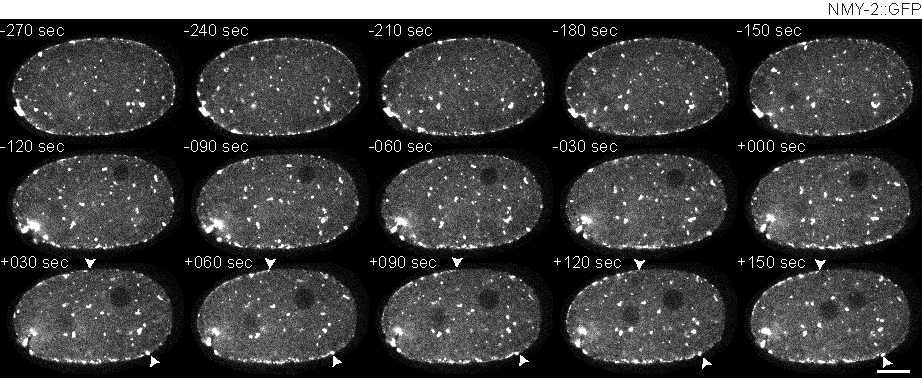
\includegraphics[width=\textwidth]{Results/FigExpMlc4/mlc4Micrograph.pdf}
\caption[Representative micrograph: \geneExp{mlc-4} \acs{rnai} embryos]{Representative \geneExp{mlc-4} \ac{rnai} embryo of SWG070 strain, labelled with \flurophoreLabel{\ac{nmy2}}{\ac{gfp}} (white), showing that male pronucleus does not posteriorise in \geneExp{mlc-4} \ac{rnai} embryos, where cortical flows are impaired. White arrows denote the depletion of myosin at the \ac{ppar} domain, which does not re-orient towards the posterior end even after t = \SI{0}{\second}. The male pronucleus can be visualized as the dark circle in the myosin channel towards the posterior end (right). t = \SI{0}{\second} is set at the end of posteriorisation of the male pronucleus -- as syncronised with the movies from unperturbed embryos of SWG070 strain. Scale bar: \SI{10}{\unitLength}. Images are rotated such that anterior and posterior ends are to the left and right respectively.}
\label{fig:swg070Mlc4Micrograph}
\end{figure}

As discussed in \autoref{sec:ApAxisEstablishment}, cortical flows play an important role in proper \ac{ap} axis establishment. A prime question to ask then is if cortical flows also play a role in \ac{ap} axis alignment. The role of cortical flows in \ac{ap} axis alignment could be understood by observing posteriorisation of the male pronucleus in embryos with impaired cortical flows. To generate embryos with reduced cortical flow velocity, \ac{rnai} of \geneExp{mlc-4} on worms of SWG070 strain was performed for a feeding time of \SI{24}{\unitRNAiTime} (see \autoref{sec:rnaiMethods} for details on \ac{rnai}). MLC-4 is a conserved regulatory light chain present in \ac{nmy2}, and is required for the \ac{nmy2} myosin motor to function \citep{shelton1999nonmuscle}. Cortical flows were found to be indeed reduced in \geneExp{mlc-4} \ac{rnai} embryos -- an average cortical flow speed of \SI{1.45 +- 0.30}{\unitCrtxVel} in \geneExp{mlc-4} \ac{rnai} embryos compared to \SI{4.12 +- 0.59}{\unitCrtxVel} in unperturbed control embryos was observed.

\begin{table}
    \centering
    \begin{tabular}{|C{0.3\textwidth}|C{0.3\textwidth}|C{0.3\textwidth}|}
        \hline
        Experimental Condition & Strain & Avg. cortical flow speed (\si{\unitCrtxVel})\\
        \hline
        Unperturbed & SWG070 & \num{4.12 +- 0.59}\\
        \geneExp{mlc-4} \ac{rnai} & SWG070 & \num{1.45 +- 0.30}\\
        \geneExp{nop-1} \ac{rnai} & SWG070 & \num{2.89 +- 0.65}\\
        \geneExp{nop-1; mel-11} \ac{rnai} & SWG070 & \num{3.34 +- 0.52}\\
        \geneExp{ima-3} \ac{rnai} & SWG070 & \num{3.99 +- 0.51}\\
        \geneExp{air-1} \ac{rnai} & SWG070 & \num{3.04 +- 0.84}\\
        \hline
        Unperturbed & SWG057 & 2.84 +- 0.37\\
        \geneExp{goa-1; gpa-16} \ac{rnai} & SWG057 & 2.62 +- 0.52\\
        \hline
    \end{tabular}
    \caption{Cortical flow speeds measured in different experimental conditions described in \autoref{ch:Results}. Average cortical flow speeds $\pm$ standard deviation are reported.}
    \label{tab:resultsCorticalFlowSpeeds}
\end{table}

\begin{figure}
\centering
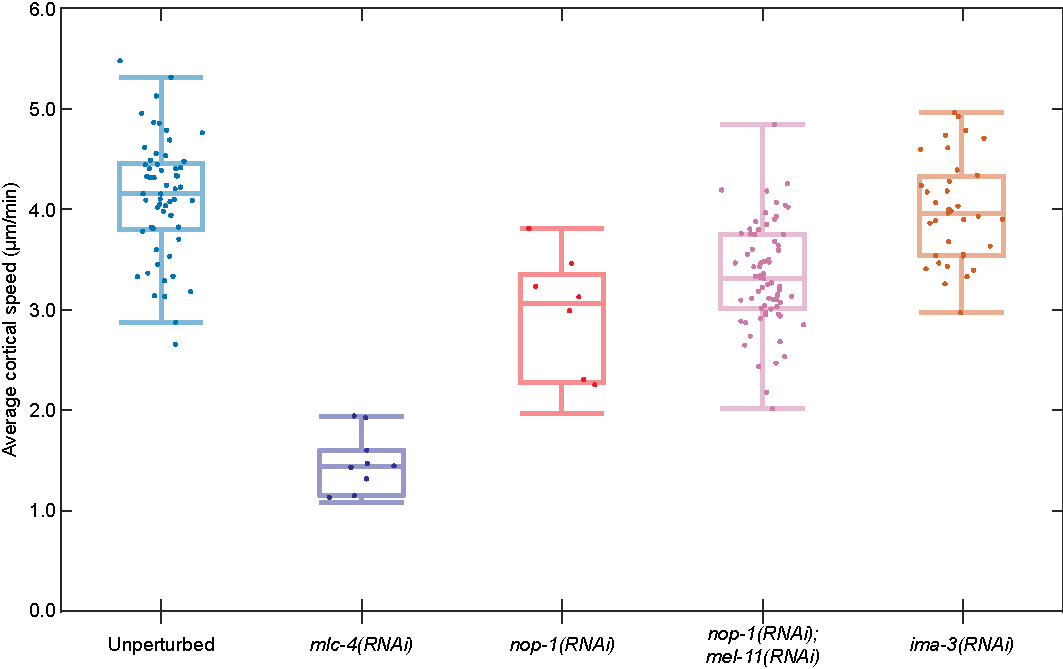
\includegraphics[width=\textwidth]{Results/FigExpCorticalFlows/crtxFlowSpeed.pdf}
\caption[Comparison of average cortical flow speed between different experimental conditions]{Average cortical flow speeds observed in different experimental conditions. Cortical flow speeds are averaged over all positions at all times for all embryos in given experimental condition. Also see \autoref{tab:resultsCorticalFlowSpeeds}}
\label{fig:resultsCorticalFlowSpeeds}
\end{figure}

\begin{figure}
\centering
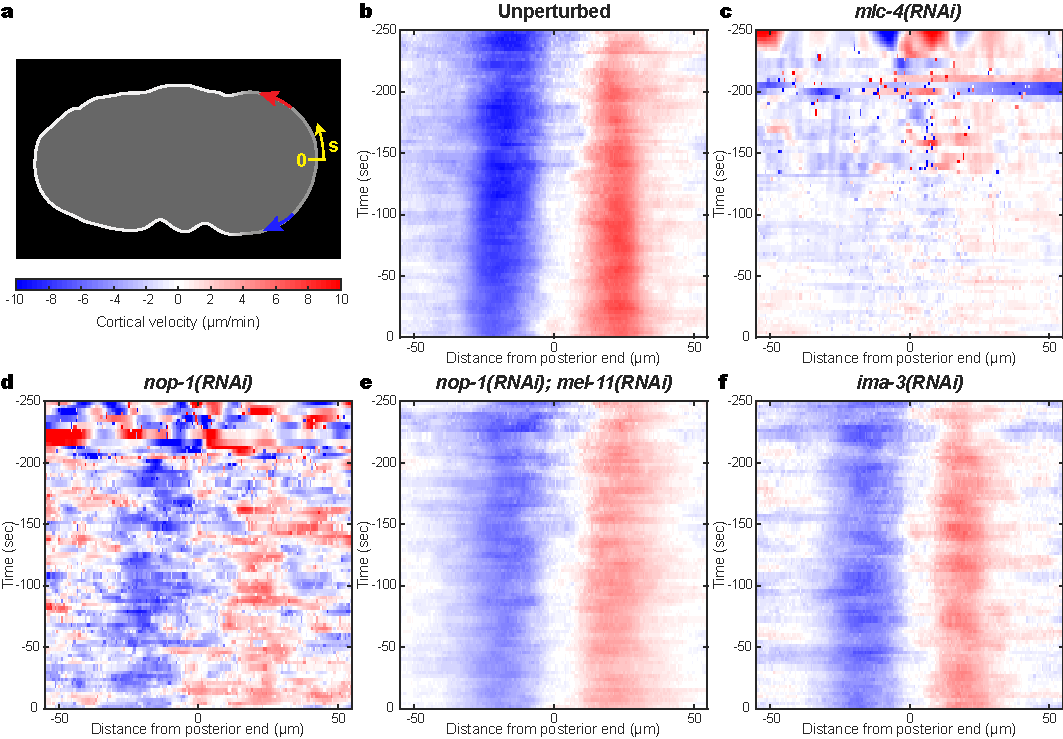
\includegraphics[width=\textwidth]{Results/FigExpCorticalFlows/crtxFlowTime.pdf}
\caption[Comparing cortical flows between different experimental conditions vs time]{Average cortical flow velocity (color, in \si{\unitCrtxVel}) plotted as a function of time (along y-axis, in \si{\second}, t = \SI{0}{\second} denotes end of posteriorization) and position on the cortex (along x-axis, in \si{\unitLength}, s=\SI{0}{\unitLength} denotes posterior end), as observed in different experimental conditions. Average cortical flow velocity at a given time and position on the cortex is obtained by averaging over cortical flows measured in all embryos at the given time and position on the cortex -- see \autoref{sec:statAnalysis}. a) Schematic. s denotes the position on the cortex, as measured along the arclength of the cortex from the posterior end (s=\SI{0}{\unitLength}). Distances in the anti-clockwise direction are considered positive. Color bar maps the colors in the plots to cortical velocity in \si{\unitCrtxVel}. Red shades indicates cortical flow pointing in the anti-clockwise direction (i.e. along the increasing direction of $s$, denoted as positive flow velocity), and blue shades in the clockwise direction (denoted as negative flow velocity). Cortical flows for (b) unperturbed embryos (N = 57), (c) \geneExp{mlc-4} RNAi embryos  (N = 10), (d) \geneExp{nop-1} RNAi embryos  (N = 9), (e) \geneExp{nop-1; mel-11} RNAi embryos  (N = 69), and (f) \geneExp{ima3} RNAi embryos (N = 35) are plotted -- all from SWG070 strain.}
\label{fig:resultsCorticalAvgFlowVsTime}
\end{figure}

\begin{figure}
\centering
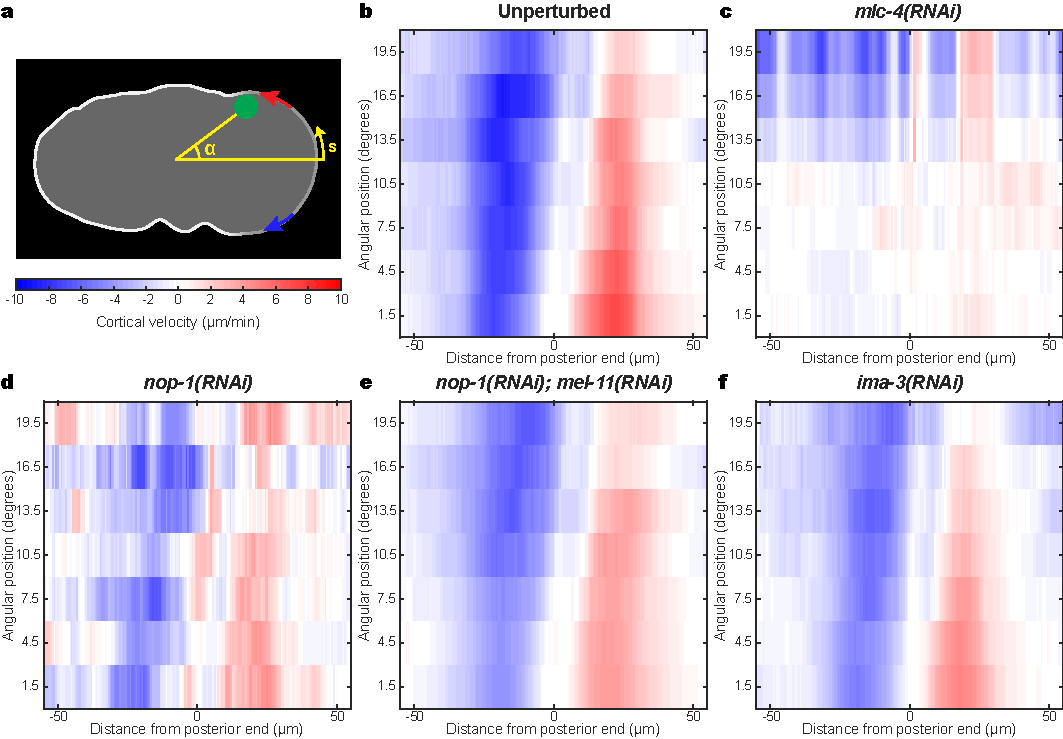
\includegraphics[width=\textwidth]{Results/FigExpCorticalFlows/crtxFlowAngle.pdf}
\caption[Comparing cortical flows between different experimental conditions vs angular positions]{Average cortical flow velocity (color, in \si{\unitCrtxVel}) plotted as a function of angular position of the male pronucleus (along y-axis, in \si{\unitAngle}) and position on the cortex (along x-axis, in \si{\unitLength}, s=\SI{0}{\unitLength} denotes posterior end), as observed in different experimental conditions. Angular positions are binned with bin width \SI{3}{\unitAngle}. Average cortical flow velocity at a given angular position bin of the male pronucleus and position on the cortex is obtained by averaging over all frames that have the corresponding angular position lie in the given angular position, at the given position on the cortex -- see \autoref{sec:statAnalysis}. a) Schematic. s denotes the position on the cortex, as measured along the arclength of the cortex from the posterior end (s=\SI{0}{\unitLength}). Distances in the anti-clockwise direction are considered positive. $\alpha$ denotes the angular position of the male pronucleus. Color bar maps the colors in the plots to cortical velocity in \si{\unitCrtxVel}. Red shades indicates cortical flow pointing in the anti-clockwise direction (i.e. along the increasing direction of $s$, denoted as positive flow velocity), and blue shades in the clockwise direction (denoted as negative flow velocity). Cortical flows for (b) unperturbed embryos (N = 57), (c) \geneExp{mlc-4} RNAi embryos  (N = 10), (d) \geneExp{nop-1} RNAi embryos  (N = 9), (e) \geneExp{nop-1; mel-11} RNAi embryos  (N = 69), and (f) \geneExp{ima3} RNAi embryos (N = 35) are plotted -- all from SWG070 strain.}
\label{fig:resultsCorticalAvgFlowVsAngle}
\end{figure}

Next, \ac{ap} axis alignment in the \geneExp{mlc-4} \ac{rnai} embryos -- in which cortical flows are impaired -- is investigated. Specifically, the posteriorisation of the male pronucleus is quantified as described before -- see \autoref{fig:swg070Mlc4Trajectories} and \autoref{fig:swg070Mlc4PostVelVsAngle}. The male pronucleus in \geneExp{mlc-4} \ac{rnai} embryos was manually tracked instead of being tracked using the image analysis pipeline described in \autoref{sec:imageAnalysis}. Posteriorisation of the male pronucleus was observed to be suppressed in these \geneExp{mlc-4} \ac{rnai} embryos: from \num{7} out of \num{10} \ac{rnai} embryos in which the male pronucleus has an initial angular position greater than \SI{5}{\unitAngle}, all were observed to fail to posteriorise -- see \autoref{fig:swg070Mlc4Trajectories}. Furthermore, almost no change is observed in angular position of the male pronucleus in \ac{rnai} embryos over time. Fitting the exponential $\alpha = \alpha_0 + \exp(-\frac{t}{t_0})$ to the plotted angular positions, as done for unperturbed embryos, results in a fit that does not converge. Instead, the best fit is found for the constant function $\alpha = \alpha_0$ with $\alpha_0 = \SI{5.45 +- 0.43}{\unitAngle}$ (see \autoref{fig:swg070Mlc4Trajectories}). Thus the migration of the male pronucleus is heavily suppressed in \geneExp{mlc-4} \ac{rnai} embryos. Such an observation is strengthened by the very slow posteriorisation velocity observed in \geneExp{mlc-4} \ac{rnai} embryos (see \autoref{fig:swg070Mlc4PostVelVsAngle} and \autoref{tab:resultsPostVelMlc4}) compared to those observed in unperturbed embryos (compare \autoref{fig:swg070WtPostVelVsAngle} and \autoref{tab:resultsPostVelUnperturbed}). Altogether, these observations lead to the conclusion that cortical flows are essential for posteriorisation of the male pronucleus, and thus \ac{ap} axis alignment.

\FloatBarrier
\begin{figure}
\centering
\begin{subfigure}[t]{0.4\textwidth}
    \centering
    \includegraphics[width=\textwidth]{Results/FigExpMlc4/mlc4Trajectories.pdf}
    \caption{Trajectories of the male pronucleus (denoted by the coordinates of its center) observed in \geneExp{mlc-4} \ac{rnai} embryos. Color represents time. x- and y-axes lie along the long and short axes of an ellipse with semi-major axis $a = \SI{26.40}{\unitLength}$ and semi-minor axis $b = \SI{16.10}{\unitLength}$. Scale bar: \SI{5}{\unitLength}}
    \label{subfig:swg070Mlc4Trajectories-tracks}
\end{subfigure}
\hfill
\begin{subfigure}[t]{0.57\textwidth}
    \centering
    \includegraphics[width=\textwidth]{Results/FigExpMlc4/mlc4Angular.pdf}
    \caption{Angular position of the male pronucleus (on y-axis, in \si{\unitAngle}) plotted as a function of time (on x-axis, in \si{\second}), in \geneExp{mlc-4} \ac{rnai} embryos. Thin grey lines represent individual trajectories, thick black line represents a constant fit to the average of these tracks: $\alpha = \alpha_0$, with $\alpha_0 = \SI{5.45 +- 0.43}{\unitAngle}$. Note that the fit excludes the outlier trajectory around \SI{30}{\unitAngle} -- however including the trajectory in the exponential or the constant fit does not qualitatively change the result.} 
    \label{subfig:swg070Mlc4Trajectories-angleVsTime}
\end{subfigure}
\caption[Experimentally observed trajectories of the male pronucleus in \geneExp{mlc-4} \acs{rnai} embryos]{Experimentally observed trajectories of the male pronucleus during posteriorisation in \geneExp{mlc-4} \ac{rnai} embryos of SWG070 strain (N = 10). Male pronucleus is manually tracked in \geneExp{mlc-4} \ac{rnai} embryos. Average semi-major and semi-minor axes lengths for \geneExp{mlc-4} \ac{rnai} embryos of SWG070 strain are used in \autoref{subfig:swg070Mlc4Trajectories-tracks} -- see \autoref{tab:resultsEmbryoGeometry}. Angular position is defined as the angle between the long axis and line connecting the centers of the male pronucleus and embryo. t = \SI{0}{\second} denotes end of posteriorisation.}
\label{fig:swg070Mlc4Trajectories}
\end{figure}

\begin{table}
    \centering
    \begin{tabular}{|C{0.2\textwidth}|C{0.45\textwidth}|C{0.2\textwidth}|}
        \hline
        Angular positions (\si{\unitAngle}) & Posteriorisation velocity (\SI{1e-1}{\unitPostVel}) & No. of embryos\\
        \hline
        \numrange{0}{3} & \num{-0.03} (\num{-0.08},\num{0.01}) & 4\\
        \numrange{3}{6} & \num{-0.02} (\num{-0.01},\num{0.05}) & 5\\
        \numrange{6}{9} & \num{-0.02} (\num{-0.07},\num{0.03}) & 3\\
        \numrange{9}{12} & \num{-0.02} (\num{-0.07},\num{0.02}) & 2\\
        \numrange{12}{15} & \num{-0.3} (\num{-0.4},\num{-0.17}) & 1\\
        \hline
    \end{tabular}
    \caption{Posteriorisation velocity measured for each angular position bin in \geneExp{mlc-4} \ac{rnai} embryos. Average posteriorisation velocity along with \num{95}\% confidence interval for the average are reported.}
    \label{tab:resultsPostVelMlc4}
\end{table}

\begin{figure}[p]
\centering
\includegraphics[width=0.95\textwidth]{Results/FigExpMlc4/mlc4PostVel.pdf}
\caption[Experimentally observed posteriorisation velocity of the male pronucleus in \geneExp{mlc-4} \acs{rnai} embryos]{Top: Posteriorization velocity of the male pronucleus (along y-axis, in \si{\unitPostVel}) plotted against its angular position, in \geneExp{mlc-4} \ac{rnai} embryos of SWG070 strain (N = 10). Negative values of the posteriorisation velocity indicate movement towards the posterior end. Angular position is binned with bin width of \SI{3}{\unitAngle}. Black circles with errors bars denote average posteriorization velocity with \num{95}\% confidence intervals in each angular position bin. Grey circles represent data scatter -- measured posteriorization velocities for different angular positions in each embryo (calculated as described in \autoref{subsec:nucleusTracking} after manual tracking). Bottom: Histogram of the number of movies (along y-axis) contributing to each angular position (along x-axis) bin. A movie contributes to an angular position bin if it has any frames with angular positions within that bin. Note that a movie can contribute to multiple bins, as it may contain frames spanning different angular positions. Data was only available until \SI{15}{\unitAngle}}
\label{fig:swg070Mlc4PostVelVsAngle}
\end{figure}

\FloatBarrier
\section{Role of Pseudocleavage furrow in \acs{ap} axis alignment}\label{sec:PcFurrowRole}
As discussed in \autoref{subsec:ApAxisAlignment}, cortical flows during \ac{ap} axis establishment can lead to two consequences -- flows within the bulk cytoplasm \citep{niwayama2011hydrodynamic} and formation of the pseudocleavage furrow \citep{reymann2016cortical}. Two different mechanisms of \ac{ap} axis alignment -- cytoplasmic flow-dependent mechanism and pseudocleavage furrow-dependent mechanism -- that arise from each of the two consequence were discussed in \autoref{subsec:ApAxisAlignment}. In this section, the contributions of these two mechanisms is evaluated using experiments that remove the pseudocleavage furrow and corresponding numerical simulations of the theoretical model described in \autoref{sec:apAxisAlignmentModelMN}.

\subsection{Removing Pseudocleavage furrow via \acs{rnai}}\label{subsec:Nop1AndNop1Mel11}

\begin{figure}
\centering
\begin{subfigure}{\textwidth}
    \centering
    \includegraphics[width=\textwidth]{Results/FigExpNop1Mel11/nop1Micrograph.pdf}
    \caption{Representative \geneExp{nop-1} \ac{rnai} embryo of SWG070 strain, labelled with \flurophoreLabel{\ac{nmy2}}{\ac{gfp}} (white), showing the lack of pseudocleavage furrow in \geneExp{nop-1} \ac{rnai} embryos.}
    \label{subfig:swg070Nop1AndNop1Mel11Micrograph-nop1}
\end{subfigure}
\hfill
\begin{subfigure}{\textwidth}
    \centering
    \includegraphics[width=\textwidth]{Results/FigExpNop1Mel11/nop1mel11Micrograph.pdf}
    \caption{Representative \geneExp{nop-1; mel-11} double \ac{rnai} embryo of SWG070 strain, labelled with \flurophoreLabel{\ac{nmy2}}{\ac{gfp}} (white), showing the lack of pseudocleavage furrow in \geneExp{nop-1; mel-11} \ac{rnai} embryos.}
    \label{subfig:swg070Nop1AndNop1Mel11Micrograph-nop1mel11}
\end{subfigure}
\caption[Representative micrograph: \geneExp{nop-1} \acs{rnai} and \geneExp{nop-1; mel-11} double \acs{rnai} embryos]{Representative \geneExp{nop-1} \ac{rnai} embryo and \geneExp{nop-1; mel-11} double \ac{rnai} embryo of SWG070 strain, labelled with \flurophoreLabel{\ac{nmy2}}{\ac{gfp}} (white), showing the lack of pseudocleavage furrow in both \geneExp{nop-1} \ac{rnai} and \geneExp{nop-1; mel-11} \ac{rnai} embryos. Compare to representative unperturbed embryo depicted in \autoref{fig:swg070WtMicrograph} and pseudocleavage furrow depicted in \autoref{fig:apAxisAlignment}. The male pronucleus can be visualized as the dark circle in the myosin channel towards the posterior end. t = \SI{0}{\second} is set at the end of posteriorisation of the male pronucleus. Scale bar: \SI{10}{\unitLength} in each. Images are rotated such that anterior and posterior ends are to the left and right respectively.}
\label{fig:swg070Nop1AndNop1Mel11Micrograph}
\end{figure}

To understand the role of the pseudocleavage furrow-dependent mechanism in \ac{ap} axis alignment, posteriorisation of the male pronucleus was quantified in embryos lacking a pseudocleavage furrow. Such embryos were generated via \ac{rnai} of \geneExp{nop-1} on worms of SWG070 strain for a feeding time of \SI{24}{\unitRNAiTime} (see \autoref{sec:rnaiMethods} for details on \ac{rnai}). NOP-1 modulates activity of the small GTPase RHO-1, which is a major regulator of the activity of the actomyosin cortex in the \ac{ce} embryo \citep{tse2012nop1}. Embryos generated by worms which are mutant for NOP-1 (that is, possess a non-functional form of NOP-1) have been observed to lack a pseudocleavage furrow \citep{rose1995pseudocleavage}. While it was observed that \geneExp{nop-1} \ac{rnai} embryos do indeed lack a pseudocleavage furrow (\num{8} out of \num{9} embryos), these embryos also showed reduced cortical flow speeds, with average cortical flow speed of \SI{2.89 +- 0.65}{\unitCrtxVel} in \geneExp{nop-1} \ac{rnai} embryos compared to \SI{4.12 +- 0.59}{\unitCrtxVel} observed in unperturbed embryos (see \autoref{tab:resultsCorticalFlowSpeeds}, \autoref{fig:resultsCorticalFlowSpeeds}, \autoref{fig:resultsCorticalAvgFlowVsTime} and \autoref{fig:resultsCorticalAvgFlowVsAngle}).

To generate pseudocleavage furrow-deficient embryos with cortical flows comparable to those observed in unperturbed embryos (which do possess a pseudocleavage furrow), a double \ac{rnai} of \geneExp{nop-1} and \geneExp{mel-11} was performed on worms of SWG070 strain for a feeding time of \SI{24}{\unitRNAiTime} (see \autoref{sec:rnaiMethods} for details on double \ac{rnai}). MEL-11 is a myosin phosphatase \citep{piekny2002rho} that suppresses the activity of myosin in the cortex \citep{najafabadi2022orchestrating}. The \geneExp{nop-1; mel-11} \ac{rnai} embryos thus generated lack a pseudocleavage furrow (\num{69} out of \num{69} embryos). Furthermore, experimental measurement of cortical flows in \geneExp{nop-1; mel-11} \ac{rnai} embryos yields average cortical flow speed of \SI{3.34 +- 0.52}{\unitCrtxVel} in \geneExp{nop-1; mel-11} \ac{rnai} embryos, comparable to the average cortical flow speed \SI{4.12 +- 0.59}{\unitCrtxVel} observed in unperturbed embryos (see \autoref{tab:resultsCorticalFlowSpeeds}, \autoref{fig:resultsCorticalFlowSpeeds}, \autoref{fig:resultsCorticalAvgFlowVsTime} and \autoref{fig:resultsCorticalAvgFlowVsAngle}). Thus, the double \ac{rnai} of \geneExp{nop-1} and \geneExp{mel-11} leads to the required pseudocleavage furrow-deficient embryos with cortical flows comparable to those observed in unperturbed embryos.

Next, the \ac{ap} axis alignment process in these \geneExp{nop-1; mel-11} \ac{rnai} embryos -- which lack a pseudocleavage furrow -- is investigated. Specifically, the posteriorisation of the male pronucleus is quantified as described before -- see \autoref{fig:swg070Nop1Mel11Trajectories} and \autoref{fig:swg070Nop1Mel11PostVelVsAngle}, using the image analysis pipeline described in \autoref{sec:imageAnalysis}. Angular positions in the pseudocleavage furrow-deficient embryos were generally observed to decrease towards \SI{0}{\unitAngle} as time reaches closer to end of posteriorisation (t = \SI{0}{\second}), albeit at a slower rate compared to that observed for unperturbed embryos (\autoref{fig:swg070Nop1Mel11Trajectories}). Specifically, this decay towards \SI{0}{\unitAngle} was quantified by fitting an exponential $\alpha = \alpha_0 + \exp(-\frac{t}{t_0})$ to the plotted angular positions, yielding a time constant $t_0 = \SI{201 +- 24}{\second}$ and $\alpha_0 = \SI{-0.75 +- 0.3}{\unitAngle}$ (\autoref{fig:swg070Nop1Mel11Trajectories}). Note that the time constant $t_0 = \SI{201 +- 24}{\second}$ for the pseudocleavage furrow-deficient embryos is larger than that found for the unperturbed embryos $t_0 = \SI{119 +- 3}{\second}$ -- indicating a slower posteriorisation of the male pronucleus in the pseudocleavage furrow-deficient embryos compared to that observed in unperturbed embryos. 

\begin{figure}
\centering
\begin{subfigure}[t]{0.4\textwidth}
    \centering
    \includegraphics[width=\textwidth]{Results/FigExpNop1Mel11/nop1mel11Trajectories.pdf}
    \caption{Trajectories of the male pronucleus (denoted by the coordinates of its center) observed in \geneExp{nop-1; mel-11} \ac{rnai} embryos. Color represents time. x- and y-axes lie along the long and short axes of an ellipse with semi-major axis $a = \SI{26.4}{\unitLength}$ and semi-minor axis $b = \SI{16.1}{\unitLength}$. Scale bar: \SI{5}{\unitLength}}
    \label{subfig:swg070Nop1Mel11Trajectories-tracks}
\end{subfigure}
\hfill
\begin{subfigure}[t]{0.57\textwidth}
    \centering
    \includegraphics[width=\textwidth]{Results/FigExpNop1Mel11/nop1mel11Angular.pdf}
    \caption{Angular position of the male pronucleus (on y-axis, in \si{\unitAngle}) plotted as a function of time (on x-axis, in \si{\second}), in \geneExp{nop-1; mel-11} \ac{rnai} embryos. Thin grey lines represent individual trajectories, thick black line represents a exponential fit to the average of these tracks: $\alpha = \alpha_0 + \exp(-\frac{t}{t_0})$, with $t_0 = \SI{201 +- 24}{\second}$ and $\alpha_0 = \SI{-0.75 +- 0.3}{\unitAngle}$.} 
    \label{subfig:swg070Nop1Mel11Trajectories-angleVsTime}
\end{subfigure}
\caption[Experimentally observed trajectories of the male pronucleus in \geneExp{nop-1; mel-11} embryos]{Experimentally observed trajectories of the male pronucleus during posteriorisation in \geneExp{nop-1; mel-11} embryos of SWG070 strain (N = 69). See \autoref{subsec:nucleusTracking} for details on male pronucleus tracking. Average semi-major and semi-minor axes lengths for \geneExp{nop-1; mel-11} embryos of SWG070 strain are used in \autoref{subfig:swg070Nop1Mel11Trajectories-tracks} -- see \autoref{tab:resultsEmbryoGeometry}. Angular position is defined as the angle between the long axis and line connecting the centers of the male pronucleus and embryo. t = \SI{0}{\second} denotes end of posteriorisation.}
\label{fig:swg070Nop1Mel11Trajectories}
\end{figure}

Posteriorisation velocity of the male pronucleus in the pseudocleavage furrow-deficient embryos, plotted as a function of angular position (see \autoref{sec:statAnalysis} for details on binning of angular positions), demonstrate that the male pronucleus is, on average, moving towards the posterior end (as indicated by the negative sign of the velocity) -- with higher speed at higher angular positions (\autoref{fig:swg070Nop1Mel11PostVelVsAngle}, \autoref{tab:resultsPostVelNop1Mel11}). This is qualitatively similar to the observations made for the unperturbed embryos (\autoref{fig:swg070WtPostVelVsAngle}, \autoref{tab:resultsPostVelUnperturbed}). However, on comparison with the posteriorisation velocity observed in the latter, it is observed that the posteriorisation velocity of the male pronucleus observed in the pseudocleavage furrow-deficient embryos are consistently slower that those observed in the unperturbed embryos, with larger difference between the two at higher angular positions. 

\begin{table}
    \centering
    \begin{tabular}{|C{0.2\textwidth}|C{0.55\textwidth}|C{0.2\textwidth}|}
        \hline
        Angular positions (\si{\unitAngle}) & Posteriorisation velocity (\SI{1e-1}{\unitPostVel}) & No. of embryos\\
        \hline
        \numrange{0}{3} & \num{-0.10} (\num{-0.12},\num{-0.08}) & 37\\
        \numrange{3}{6} & \num{-0.14} (\num{-0.17},\num{-0.11}) & 36\\
        \numrange{6}{9} & \num{-0.14} (\num{-0.17},\num{-0.11}) & 29\\
        \numrange{9}{12} & \num{-0.17} (\num{-0.21},\num{-0.13}) & 19\\
        \numrange{12}{15} & \num{-0.17} (\num{-0.21},\num{-0.13}) & 19\\
        \numrange{15}{18} & \num{-0.20} (\num{-0.25},\num{-0.16}) & 13\\
        \numrange{18}{21} & \num{-0.20} (\num{-0.25},\num{-0.16}) & 12\\
        \numrange{21}{24} & \num{-0.36} (\num{-0.44},\num{-0.29}) & 8\\
        \numrange{24}{27} & \num{-0.10} (\num{-0.15},\num{-0.05}) & 3\\
        \hline
    \end{tabular}
    \caption{Posteriorisation velocity measured for each angular position bin in \geneExp{nop-1; mel-11} \ac{rnai} embryos. Average posteriorisation velocity along with \num{95}\% confidence interval for the average are reported.}
    \label{tab:resultsPostVelNop1Mel11}
\end{table}

\begin{figure}[p]
\centering
\includegraphics[width=0.95\textwidth]{Results/FigExpNop1Mel11/nop1mel11PostVel.pdf}
\caption[Experimentally observed posteriorisation velocity of the male pronucleus in \geneExp{nop-1; mel-11} \acs{rnai} embryos]{Top: Posteriorization velocity of the male pronucleus (along y-axis, in \si{\unitPostVel}) plotted against its angular position, in \geneExp{nop-1; mel-11} \ac{rnai} embryos of SWG070 strain (N = 69). Negative values of the posteriorisation velocity indicate movement towards the posterior end. Angular position is binned using a bin width of \SI{3}{\unitAngle}. Black circles with errors bars denote the average posteriorization velocity with \num{95}\% confidence intervals in each angular position bin. Grey circles represent the data scatter -- the measured posteriorization velocities for different angular positions in each embryo (see \autoref{subsec:nucleusTracking}). Bottom: Histogram of the number of movies (along y-axis) contributing to each angular position (along x-axis) bin. A movie is considered to contribute to an angular position bin if it has any frames with angular positions within that bin. Note that a movie can contribute to multiple bins, as it may contain frames spanning different angular positions.}
\label{fig:swg070Nop1Mel11PostVelVsAngle}
\end{figure}

Altogether, these experimental observations indicate that the rate of \ac{ap} axis alignment is diminished in the absence of the pseudocleavage furrow. In other words, experimental removal of pseudocleavage furrow via a double \geneExp{nop-1; mel-11} \ac{rnai} indicates that the pseudocleavage furrow is important for the dynamics of \ac{ap} axis alignment, and to ensure the alignment of the \ac{ap} axis at the rate observed in the unperturbed embryos. However, the pseudocleavage furrow is not essential for \ac{ap} axis alignment -- embryos deficient in the pseudocleavage furrow can still exhibit \ac{ap} axis alignment, albeit at a slower rate.

\FloatBarrier
\subsection{Comparing numerical simulations to experimental results}\label{subsec:expVsTheoryPcFurrow}
\subsubsection{Theoretical model accounts for \acs{ap} axis alignment in unperturbed controls}\label{subsubsec:fullModelForWT}
To further probe the role of the pseudocleavage furrow in \ac{ap} axis alignment, these experimental observations are compared to numerical simulations of the theoretical model of \ac{ap} axis alignment. As described in \autoref{sec:apAxisAlignmentModelMN} and \autoref{subsec:ApAxisAlignment}, the theoretical model considers two possible mechanisms of \ac{ap} axis alignment: cytoplasmic flow-dependent mechanism, and pseudocleavage furrow-dependent mechanism. Comparisons of experimental observations in unperturbed embryos -- which possess a pseudocleavage furrow -- and \geneExp{nop-1; mel-11} \ac{rnai} embryos -- which lack a pseudocleavage furrow with numerical simulations of the theoretical model could then yield insights into the contributions of the two mechanisms to \ac{ap} axis alignment.

First, the theoretical model is compared with observations in the unperturbed embryo. Specifically, posteriorisation velocity of the male pronucleus as a function of its angular position, and the trajectory of the male pronucleus (that is, angular position as a function of time) are calculated (see \autoref{sec:apAxisAlignmentModelMN} for details) using the full theoretical model -- that is, including the pseudocleavage furrow-dependent mechanism, as unperturbed embryos possess a pseudocleavage furrow. Quantities calculated from the the theoretical model are then compared to those observed in the experiments with unperturbed embryos. 

Numerical simulations of the theoretical model requires calibration of model parameters using the experimentally measured cortical flows. Note that the model is evaluated (in this section) on an ellipsoid with the same axes lengths as the average axes lengths for the unperturbed embryos: \longAxisLength = \SI{28.9}{\unitLength} (semi-major axis), \shortAxisLength = \SI{16.4}{\unitLength} -- see \autoref{tab:resultsEmbryoGeometry}. In brief, the calibration procedure varies the following model parameters: hydrodynamic length \hydrodynamicLength, active force relaxation \activeRelaxLength and nematic stress relaxation \nematicLength. Cortical flows calculated using the varied parameters are then compared to those experimentally measured. This is done for a range of angular positions of the male pronucleus, using the average cortical flows observed for angular position bin (with bin width of \SI{3}{\unitAngle}, shown in \autoref{fig:resultsCorticalAvgFlowVsAngle} -- see \autoref{sec:statAnalysis} for details on methodology). Angular positions upto \SI{21}{\unitAngle} only are considered for the calibration procedure, due to worse quality of data for higher angular positions as the number of movies contributing to those angular position bins decreases. The calibration procedure results in values of \hydrodynamicLength, \activeRelaxLength and \nematicLength that ensure best match with experimentally measured cortical flows. A detailed discussion on the calibration process can be found in \autoref{subsec:numericsModelMN}. 

\begin{figure}
    \centering
    \includegraphics[width=\textwidth]{Results/FigComparePCF/wtCorticalFlowModel.pdf}
    \caption[Calibrating theoretical model using cortical flows observed in unperturbed embryos]{Comparison of observed cortical flows in unperturbed embryos of SWG070 strain to those calculated by the theoretical model of \ac{ap} axis alignment. Blue line denotes the average cortical flow velocity observed in unperturbed embryos, plotted as a function of position along the cortex $s$ in each angular position bin -- also depicted in \autoref{fig:resultsCorticalAvgFlowVsAngle}. Red denotes the cortical flow velocity calculated by the theoretical model after calibration, with model parameters: \hydrodynamicLength = \SI{10}{\unitLength}, \activeRelaxLength = \SI{11.5}{\square\unitLength\per\second}, \nematicLength = \SI{152.5}{\square\unitLength\per\second}.}
    \label{fig:unperturbedModelCalibrationCorticalFlows}
\end{figure}

For the experimentally measured cortical flows in unperturbed embryos, the calibration procedure yields the following model parameters: \hydrodynamicLength = \SI{10}{\unitLength}, \activeRelaxLength = \SI{11.5}{\square\unitLength\per\second}, \nematicLength = \SI{152.5}{\square\unitLength\per\second} -- see \autoref{fig:unperturbedModelCalibrationCorticalFlows}. In the theoretical model, bulk cytoplasmic flows are determined uniquely from the calculated cortical flows via the no-slip boundary condition (see \autoref{subsec:cytoplasmPronucleusModelMN}). Comparison of experimentally measured cortical and cytoplasmic flows (see \autoref{subsec:corticalFlows} and \autoref{subsec:cytoFlows} for methodology) with calculated cortical and cytoplasmic flows shows a good agreement between the two -- see \autoref{fig:unperturbedModelCalibrationCorticalFlows} and \autoref{fig:unperturbedModelCalibrationCorticalAndCytoFlows}. Thus, the theoretical model can faithfully recapitulate the experimental cortical and cytoplasmic flows, for the selected set of model parameters.

\begin{figure}
    \centering
    \includegraphics{Results/FigComparePCF/cytoFlowCompare.pdf}
    \caption[Flows observed in unperturbed embryos compared to those calculated by theoretical model]{Comparison of observed cortical and cytoplasmic flows in unperturbed embryos of SWG070 strain (left) to those calculated by the theoretical model of \ac{ap} axis alignment (right) with model parameters: \hydrodynamicLength = \SI{10}{\unitLength}, \activeRelaxLength = \SI{11.5}{\square\unitLength\per\second}, \nematicLength = \SI{152.5}{\square\unitLength\per\second} (referred to as the unperturbed model), for three angular positions (\SI{0}{\unitAngle}, \SI{5}{\unitAngle}, \SI{10}{\unitAngle}) of the male pronucleus (black shaded circle).In each panel, ellipse interior represents cytoplasmic flows, and outer ellipse represents cortical flows. See colorbar for magnitude of flow velocities.}
    \label{fig:unperturbedModelCalibrationCorticalAndCytoFlows}
\end{figure}

Comparison of the experimentally observed posteriorisation velocity of the male pronucleus with those calculated using the model fix the final model parameter \dragCoefficient. This parameter captures the direct interactions between the male pronucleus and the cortex (see \autoref{subsec:cytoplasmPronucleusModelMN}). For the set of model parameters obtained via calibration for the unperturbed embryos, \dragCoefficient = \num{0.61} to ensure that the calculated posteriorisation velocity best match the observed posteriorization velocity as a function of angular position of the male pronucleus -- see \autoref{subfig:unperturbedModelCompareExpt-postVel} and \autoref{tab:resultsPostVelUnperturbedVsFullModel}. With these model parameters, the calculated posteriorisation velocity agrees with experimentally observed average posteriorisation velocity in unperturbed embryos, for angular positions upto \SI{21}{\unitAngle}. For higher angular positions, average posteriorisation velocity observed in experiments is faster compared to calculated posteriorisation velocity for the same angular position. By integrating the calculated posteriorisation velocity (as a function of angular position), the calculated trajectory of the male pronucleus -- referring to the calculated angular position of the male pronucleus as a function of time relative to end of posteriorisation -- can also be obtained (see \autoref{subsec:numericsModelMN}), which is observed to agree well with the experimentally observed trajectories of the male pronucleus -- see \autoref{subfig:unperturbedModelCompareExpt-tracks}.

\begin{table}
    \centering
    \begin{tabular}{|C{0.2\textwidth}|C{0.35\textwidth}|C{0.35\textwidth}|}
        \hline
        Angular positions (\si{\unitAngle}) & Experimental post. velocity (\SI{1e-1}{\unitPostVel}) & Calculated post. velocity (\SI{1e-1}{\unitPostVel})\\
        \hline
        \numrange{0}{3} & \num{-0.15} (\num{-0.18},\num{-0.13}) & \num{-0.09}\\
        \numrange{3}{6} & \num{-0.17} (\num{-0.20},\num{-0.14}) & \num{-0.22}\\
        \numrange{6}{9} & \num{-0.27} (\num{-0.30},\num{-0.23}) & \num{-0.30}\\
        \numrange{9}{12} & \num{-0.40} (\num{-0.46},\num{-0.35}) & \num{-0.38}\\
        \numrange{12}{15} & \num{-0.46} (\num{-0.52},\num{-0.41}) & \num{-0.45}\\
        \numrange{15}{18} & \num{-0.40} (\num{-0.47},\num{-0.34}) & \num{-0.47}\\
        \numrange{18}{21} & \num{-0.49} (\num{-0.58},\num{-0.40}) & \num{-0.48}\\
        \numrange{21}{24} & \num{-0.85} (\num{-0.98},\num{-0.72}) & \num{-0.47}\\
        \hline
    \end{tabular}
    \caption{Experimentally observed posteriorisation velocity for each angular position bin in unperturbed embryos compared with those calculated by the unperturbed model (theoretical model evaluated with model parameters: \hydrodynamicLength = \SI{10}{\unitLength}, \activeRelaxLength = \SI{11.5}{\square\unitLength\per\second}, \nematicLength = \SI{152.5}{\square\unitLength\per\second}, \dragCoefficient = \num{0.61}). Experimental Post. velocity: Average posteriorisation velocity along with \num{95}\% confidence interval for each angular position bin observed in unperturbed embryos (see \autoref{tab:resultsPostVelUnperturbed} and \autoref{fig:swg070WtPostVelVsAngle}. Calculated Post. velocity: Posteriorisation velocity calculated at center of angular position bin by theoretical model with model parameters: \hydrodynamicLength = \SI{10}{\unitLength}, \activeRelaxLength = \SI{11.5}{\square\unitLength\per\second}, \nematicLength = \SI{152.5}{\square\unitLength\per\second}, \dragCoefficient = \num{0.61}.}
    \label{tab:resultsPostVelUnperturbedVsFullModel}
\end{table}

\begin{figure}
    \centering
    \begin{subfigure}[t]{0.45\textwidth}
        \includegraphics[width=\textwidth]{Results/FigComparePCF/wtPostVelModel.pdf}
        \caption{Comparing average posteriorisation velocity of the male pronucleus (black circles with error bars, \num{95}\% confidence interval) in unperturbed embryos (from \autoref{fig:swg070WtPostVelVsAngle}) with that calculated by unperturbed model (black line), both plotted against angular position of the male pronucleus. Posteriorisation velocity is on y-axis (in \si{\unitPostVel}, negative velocity indicate movement towards posterior end), and angular position on x-axis (in \si{\unitAngle}).}
        \label{subfig:unperturbedModelCompareExpt-postVel}
    \end{subfigure}
    \hfill
    \begin{subfigure}[t]{0.45\textwidth}
        \includegraphics[width=\textwidth]{Results/FigComparePCF/wtTrajectoriesModel.pdf}
        \caption{Comparing angular positions of the male pronucleus (y-axis, in \si{\unitAngle}) observed in unperturbed embryos (thin grey lines, from \autoref{fig:swg070WtTrajectories}) with the calculated trajectory of the male pronucleus (thick black line) from unperturbed model, both plotted against time (on x-axis, in \si{\second}, t = \SI{0}{\second} denotes end of posteriorisation).}
        \label{subfig:unperturbedModelCompareExpt-tracks}
    \end{subfigure}
    \caption[Experimentally observed posteriorisation in unperturbed embryos compared with that calculated by theoretical model]{Comparing experimentally observed posteriorisation of the male pronucleus in unperturbed embryos of the SWG070 strain with that calculated by the unperturbed model. Unperturbed model refers to the theoretical model of \ac{ap} axis alignment evaluated with the following model parameters: \hydrodynamicLength = \SI{10}{\unitLength}, \activeRelaxLength = \SI{11.5}{\square\unitLength\per\second}, \nematicLength = \SI{152.5}{\square\unitLength\per\second}, \dragCoefficient = \num{0.61}. \dragCoefficient = \num{0.61} is selected to best match the average posteriorisation velocity observed in unperturbed embryos of the SWG070 strain, depicted in \autoref{subfig:unperturbedModelCompareExpt-postVel}.}
    \label{fig:unperturbedModelCompareExpt}
\end{figure} 

The sensitivity of the calculated posteriorisation velocity to the calibrated model parameters was also investigated. Specifically, \hydrodynamicLength and \nematicLength were separately varied to $\pm\num{50}\%$ of their calibrated values -- see \autoref{fig:unperturbedModelParameterVary}, \autoref{tab:resultsPostVelFullModelVaryLh} and \autoref{tab:resultsPostVelFullModelVaryLn}. As discussed in \autoref{subsec:numericsModelMN}, \activeRelaxLength scales with the cortical flow velocity, and therefore is set separately. Posteriorisation velocity of the male pronucleus is then calculated using the varied model parameters and then compared again to those experimentally measured in unperturbed embryos. It is observed that the calculated posteriorisation velocity still retain similar qualitative features as those experimentally measured in unperturbed embryos: Posteriorisation velocity calculated after model parameter variation remain comparable to the average posteriorisation velocity observed in experiments for angular positions upto \SI{21}{\unitAngle}. Thus, the calculated posteriorisation velocity is robust to variations in the calibration procedure.

Of note also is the hydrodynamic length \hydrodynamicLength, whose value have been measured in previous studies \citep{saha2016determining,mayer2010anisotropies}. Here, a hydrodynamic length of \hydrodynamicLength = \SI{10}{\unitLength} is observed for the unperturbed embryo, which is close to the previous measurements of the hydrodynamic length ($\sim$\SI{14}{\unitLength} \citep{saha2016determining,mayer2010anisotropies}). Additionally, the model parameter variation considered before indicates that the calculated posteriorisation velocity is robust towards variation in \hydrodynamicLength. Thus, the calibrated hydrodynamic length used in theoretical model here is in agreement with the previously observed measurements of the hydrodynamic length of the cortex. 

\begin{table}
    \centering
    \begin{tabular}{|C{0.2\textwidth}|C{0.35\textwidth}|C{0.35\textwidth}|}
        \hline
        Angular positions (\si{\unitAngle}) & \multicolumn{2}{c|}{Calculated posteriorisation velocity (\SI{1e-1}{\unitPostVel})}\\
        \cline{2-3}
        & \hydrodynamicLength $\coloneqq$ \num{1.5}\hydrodynamicLength & \hydrodynamicLength $\coloneqq$ \num{0.5}\hydrodynamicLength\\
        \hline
        \numrange{0}{3} & \num{-0.08} & \num{-0.11}\\
        \numrange{3}{6} & \num{-0.18} & \num{-0.25}\\
        \numrange{6}{9} & \num{-0.25} & \num{-0.34}\\
        \numrange{9}{12} & \num{-0.32} & \num{-0.43}\\
        \numrange{12}{15} & \num{-0.38} & \num{-0.50}\\
        \numrange{15}{18} & \num{-0.40} & \num{-0.53}\\
        \numrange{18}{21} & \num{-0.40} & \num{-0.53}\\
        \numrange{21}{24} & \num{-0.40} & \num{-0.52}\\
        \hline
    \end{tabular}
    \caption{Posteriorisation velocity calculated (at center of angular position bin) using unperturbed model after varying \hydrodynamicLength, for different angular positions. Unperturbed model refers to theoretical model evaluated with model parameters: \hydrodynamicLength = \SI{10}{\unitLength}, \activeRelaxLength = \SI{11.5}{\square\unitLength\per\second}, \nematicLength = \SI{152.5}{\square\unitLength\per\second}, \dragCoefficient = \num{0.61}. Second column uses \hydrodynamicLength = \SI{15}{\unitLength} instead, and third column \hydrodynamicLength = \SI{5}{\unitLength} instead.}
    \label{tab:resultsPostVelFullModelVaryLh}
\end{table}

\begin{table}
    \centering
    \begin{tabular}{|C{0.2\textwidth}|C{0.35\textwidth}|C{0.35\textwidth}|}
        \hline
        Angular positions (\si{\unitAngle}) & \multicolumn{2}{c|}{Calculated posteriorisation velocity (\SI{1e-1}{\unitPostVel})}\\
        \cline{2-3}
        & \nematicLength $\coloneqq$ \num{1.5}\nematicLength & \nematicLength $\coloneqq$ \num{0.5}\nematicLength\\
        \hline
        \numrange{0}{3} & \num{-0.10} & \num{-0.08}\\
        \numrange{3}{6} & \num{-0.25} & \num{-0.18}\\
        \numrange{6}{9} & \num{-0.34} & \num{-0.24}\\
        \numrange{9}{12} & \num{-0.43} & \num{-0.30}\\
        \numrange{12}{15} & \num{-0.50} & \num{-0.36}\\
        \numrange{15}{18} & \num{-0.54} & \num{-0.37}\\
        \numrange{18}{21} & \num{-0.54} & \num{-0.37}\\
        \numrange{21}{24} & \num{-0.54} & \num{-0.37}\\
        \hline
    \end{tabular}
    \caption{Posteriorisation velocity calculated (at center of angular position bin) using unperturbed model after varying \nematicLength, for different angular positions. Unperturbed model refers to theoretical model evaluated with model parameters: \hydrodynamicLength = \SI{10}{\unitLength}, \activeRelaxLength = \SI{11.5}{\square\unitLength\per\second}, \nematicLength = \SI{152.5}{\square\unitLength\per\second}, \dragCoefficient = \num{0.61}. Second column uses \nematicLength = \SI{228.75}{\unitLength} instead, and third column \nematicLength = \SI{76.25}{\unitLength} instead.}
    \label{tab:resultsPostVelFullModelVaryLn}
\end{table}

\begin{figure}
    \centering
    \begin{subfigure}[t]{0.45\textwidth}
        \includegraphics[width=\textwidth]{Results/FigComparePCF/wtPostVelModelLhVary.pdf}
        \caption{Varying \hydrodynamicLength between [\SI{5}{\unitLength},\SI{15}{\unitLength}]. Increasing \hydrodynamicLength leads to slower posteriorisation velocity.}
        \label{subfig:unperturbedModelParameterVary-Lh}
    \end{subfigure}
    \hfill
    \begin{subfigure}[t]{0.45\textwidth}
        \includegraphics[width=\textwidth]{Results/FigComparePCF/wtPostVelModelLnVary.pdf}
        \caption{Varying \nematicLength between [\SI{76.25}{\unitLength},\SI{228.75}{\unitLength}]. Increasing \nematicLength leads to faster posteriorisation velocity.}
        \label{subfig:unperturbedModelParameterVary-Ln}
    \end{subfigure}
    \caption[Effect of model parameter variation on calculated posteriorisation velocity]{Posteriorisation velocity of the male pronucleus calculated by the unperturbed model (theoretical model evaluated with model parameters: \hydrodynamicLength = \SI{10}{\unitLength}, \activeRelaxLength = \SI{11.5}{\square\unitLength\per\second}, \nematicLength = \SI{152.5}{\square\unitLength\per\second}, \dragCoefficient = \num{0.61}) is robust to variation in \hydrodynamicLength and \nematicLength. Comparison of the calculated posteriorisation velocity using calibrated model parameters (black line), calculated posteriorisation velocity with \hydrodynamicLength $\coloneqq$ \num{1.5}\hydrodynamicLength (\autoref{subfig:unperturbedModelParameterVary-Lh}, red dashed line) or \nematicLength $\coloneqq$ \num{1.5}\nematicLength (\autoref{subfig:unperturbedModelParameterVary-Ln}, red dashed line), calculated posteriorisation velocity with \hydrodynamicLength $\coloneqq$ \num{1.5}\hydrodynamicLength (\autoref{subfig:unperturbedModelParameterVary-Lh}, blue dashed line) or \nematicLength $\coloneqq$ \num{0.5}\nematicLength (\autoref{subfig:unperturbedModelParameterVary-Ln}, blue dashed line), and average posteriorisation velocity observed in unperturbed embryos (black circles with error bars, \num{95}\% confidence interval). Posteriorisation velocity is plotted on the y-axis in \si{\unitPostVel} against angular position on the x-axis in \si{\unitAngle}.}
    \label{fig:unperturbedModelParameterVary}
\end{figure}

Therefore, the full model (with both mechanisms included) can -- both qualitatively and quantitatively -- recapitulate the observed \ac{ap} axis alignment process in the unperturbed embryos, using the set of model parameters selected here: \hydrodynamicLength = \SI{10}{\unitLength}, \activeRelaxLength = \SI{11.5}{\square\unitLength\per\second}, \nematicLength = \SI{152.5}{\square\unitLength\per\second}, \dragCoefficient = \num{0.61}. The model evaluated with this set of model parameters will be referred to as the unperturbed model.

\FloatBarrier
\subsubsection{Eliminating role of pseudocleavage furrow-dependent mechanism in model explains the slower \acs{ap} axis alignment in pseudocleavage furrow-deficient embryos}\label{subsubsec:cytoModelForNop1Mel11}

Next, the theoretical model is compared with observations in the pseudocleavage furrow-deficient embryos generated by \geneExp{nop-1; mel-11} double \ac{rnai}. To mimic the experimental removal of the pseudocleavage furrow in the model, \nematicLength -- the model parameter that controls the contribution of the pseudocleavage-furrow dependent mechanism in the model (see \autoref{subsec:numericsModelMN}) -- is fixed to \SI{0}{\square\unitLength\per\second}. Due to this, and since the cortical flows in these embryos are similar but not identical to those observed in unperturbed embryos, the model is recalibrated to ensure cortical flows observed in the \geneExp{nop-1; mel-11} \ac{rnai} embryos are captured by the model. In this recalibration, only \activeRelaxLength is varied. Doing so yields the following model parameters: \hydrodynamicLength = \SI{10}{\unitLength}, \activeRelaxLength = \SI{7}{\square\unitLength\per\second}, \nematicLength = \SI{0}{\square\unitLength\per\second}. The value for the drag coefficient \dragCoefficient = \num{0.61} as determined for the unperturbed embryos is retained here. The model evaluated with this set of model parameters will be referred to as the pseudocleavage furrow-deficient model.

\begin{figure}
    \centering
    \includegraphics[width=\textwidth]{Results/FigComparePCF/nopMelCorticalFlowModel.pdf}
    \caption[Calibrating theoretical model using cortical flows observed in pseudocleavage furrow-deficient embryos]{Comparison of observed cortical flows in pseudocleavage furrow-deficient embryos generated using \geneExp{nop-1; mel-11} \ac{rnai} in SWG070 strain to those calculated by the theoretical model of \ac{ap} axis alignment, with setting \nematicLength = \SI{0}{\square\unitLength\per\second}. Blue line denotes the average cortical flow velocity observed in \geneExp{nop-1; mel-11} \ac{rnai} embryos, plotted as a function of position along the cortex $s$ in each angular position bin -- also depicted in \autoref{fig:resultsCorticalAvgFlowVsAngle}. Red denotes the cortical flow velocity calculated by the theoretical model after calibration, with model parameters: \hydrodynamicLength = \SI{10}{\unitLength}, \activeRelaxLength = \SI{7}{\square\unitLength\per\second}, \nematicLength = \SI{0}{\square\unitLength\per\second}.}
    \label{fig:pcfRemovedModelCalibrationCorticalFlows}
\end{figure}

Before a comparison with experimental data is made, the posteriorisation velocity calculated using the unperturbed model and the pseudocleavage-deficient model are compared (compare \autoref{subfig:pcfRemoveModelCompareExpt-postVel} with \autoref{subfig:unperturbedModelCompareExpt-postVel}). At each angular position, the pseudocleavage furrow-deficient model calculates slower posteriorisation velocity compared to the unperturbed model -- with the difference larger for higher angular positions. This is qualitatively similar to what was observed experimentally observed -- pseudocleavage furrow-deficient embryos (generated using \geneExp{nop-1; mel-11} \ac{rnai}) exhibit slower average posteriorisation velocities compared to unperturbed embryos at all angular positions observed in experiments -- with larger difference at higher angular positions (compare \autoref{fig:swg070WtPostVelVsAngle} to \autoref{fig:swg070Nop1Mel11PostVelVsAngle}). Direct comparison between the calculated posteriorisation velocity from the pseudocleavage furrow-deficient embryo to the experimental posteriorisation velocity observed in pseudocleavage furrow-deficient embryos (generated using \geneExp{nop-1; mel-11} \ac{rnai}) reveals that the calculated posteriorisation velocity broadly match the experimentally observed ones in the pseudocleavage furrow-deficient embryos -- see \autoref{subfig:pcfRemoveModelCompareExpt-postVel} and \autoref{tab:resultsPostVelNop1Mel11VsPcfRemoveModel}. Specifically, the pseudocleavage furrow-deficient model calculates posteriorisation velocity which are slightly slower, but still comparable to those observed in the pseudocleavage furrow-deficient embryos. As before, the calculated posteriorisation velocity may be integrated over to obtain a calculated trajectory of the male pronucleus using the pseudocleavage furrow-deficient model (see \autoref{subsec:numericsModelMN}). Comparison with experimentally observed trajectories in the pseudocleavage furrow-deficient embryo shows that the calculated trajectory agrees well with the experimentally observed trajectories of the male pronucleus observed in pseudocleavage furrow-deficient embryos -- see \autoref{subfig:pcfRemoveModelCompareExpt-tracks}.

\begin{table}
    \centering
    \begin{tabular}{|C{0.2\textwidth}|C{0.35\textwidth}|C{0.35\textwidth}|}
        \hline
        Angular positions (\si{\unitAngle}) & Experimental post. velocity (\SI{1e-1}{\unitPostVel}) & Calculated post. velocity (\SI{1e-1}{\unitPostVel})\\
        \hline
        \numrange{0}{3} & \num{-0.10} (\num{-0.12},\num{-0.08}) & \num{-0.03}\\
        \numrange{3}{6} & \num{-0.14} (\num{-0.17},\num{-0.11}) & \num{-0.07}\\
        \numrange{6}{9} & \num{-0.14} (\num{-0.17},\num{-0.11}) & \num{-0.08}\\
        \numrange{9}{12} & \num{-0.17} (\num{-0.21},\num{-0.13}) & \num{-0.11}\\
        \numrange{12}{15} & \num{-0.17} (\num{-0.21},\num{-0.13}) & \num{-0.12}\\
        \numrange{15}{18} & \num{-0.20} (\num{-0.25},\num{-0.16}) & \num{-0.12}\\
        \numrange{18}{21} & \num{-0.20} (\num{-0.25},\num{-0.16}) & \num{-0.12}\\
        \numrange{21}{24} & \num{-0.36} (\num{-0.44},\num{-0.29}) & \num{-0.11}\\
        \hline
    \end{tabular}
    \caption{Experimentally observed posteriorisation velocity for each angular position bin in pseudocleavage furrow-deficient embryos generated using \geneExp{nop-1; mel-11} \ac{rnai} compared with those calculated by the pseudocleavage furrow-deficient model (theoretical model evaluated with model parameters: \hydrodynamicLength = \SI{10}{\unitLength}, \activeRelaxLength = \SI{7}{\square\unitLength\per\second}, \nematicLength = \SI{0}{\square\unitLength\per\second}, \dragCoefficient = \num{0.61}). Experimental Post. velocity: Average posteriorisation velocity along with \num{95}\% confidence interval for each angular position bin observed in \geneExp{nop-1; mel-11} \ac{rnai} embryos (see \autoref{tab:resultsPostVelNop1Mel11} and \autoref{fig:swg070Nop1Mel11PostVelVsAngle}. Calculated Post. velocity: Posteriorisation velocity calculated at center of angular position bin by theoretical model with model parameters: \hydrodynamicLength = \SI{10}{\unitLength}, \activeRelaxLength = \SI{7}{\square\unitLength\per\second}, \nematicLength = \SI{0}{\square\unitLength\per\second}, \dragCoefficient = \num{0.61}.}
    \label{tab:resultsPostVelNop1Mel11VsPcfRemoveModel}
\end{table}

\begin{figure}
    \centering
    \begin{subfigure}[t]{0.45\textwidth}
        \includegraphics[width=\textwidth]{Results/FigComparePCF/nopMelPostVelModel.pdf}
        \caption{Comparing average posteriorisation velocity of the male pronucleus (black circles with error bars, \num{95}\% confidence interval) in pseudocleavage furrow-deficient embryos (from \autoref{fig:swg070Nop1Mel11PostVelVsAngle}) with that calculated by pseudocleavage furrow-deficient model (black line), both plotted against angular position of the male pronucleus. Posteriorisation velocity is on y-axis (in \si{\unitPostVel}, negative velocity indicate movement towards posterior end), and angular position on x-axis (in \si{\unitAngle}).}
        \label{subfig:pcfRemoveModelCompareExpt-postVel}
    \end{subfigure}
    \hfill
    \begin{subfigure}[t]{0.45\textwidth}
        \includegraphics[width=\textwidth]{Results/FigComparePCF/wtTrajectoriesModel.pdf}
        \caption{Comparing angular positions of the male pronucleus (y-axis, in \si{\unitAngle}) observed in pseudocleavage furrow-deficient embryos (thin grey lines, from \autoref{fig:swg070Nop1Mel11Trajectories}) with the calculated trajectory of the male pronucleus (thick black line) from pseudocleavage furrow-deficient model, both plotted against time (on x-axis, in \si{\second}, t = \SI{0}{\second} denotes end of posteriorisation).}
        \label{subfig:pcfRemoveModelCompareExpt-tracks}
    \end{subfigure}
    \caption[Experimentally observed posteriorisation in pseudocleavage furrow-deficient embryos compared with that calculated by theoretical model]{Comparing experimentally observed posteriorisation of the male pronucleus in pseudocleavage furrow-deficient embryos generated by \geneExp{nop-1; mel-11} \ac{rnai} in SWG070 strain with that calculated by the pseudocleavage furrow-deficient model. Pseudocleavage furrow-deficient model refers to the theoretical model of \ac{ap} axis alignment evaluated with the following model parameters: \hydrodynamicLength = \SI{10}{\unitLength}, \activeRelaxLength = \SI{7}{\square\unitLength\per\second}, \nematicLength = \SI{0}{\square\unitLength\per\second}, \dragCoefficient = \num{0.61}.}
    \label{fig:pcfRemoveModelCompareExpt}
\end{figure} 

Therefore, the pseudocleavage furrow-deficient model -- where \nematicLength is set to \SI{0}{\square\unitLength\per\second} -- can recapitulate the observed \ac{ap} axis alignment process in the pseudocleavage furrow-deficient embryos generated using \geneExp{nop-1; mel-11} \ac{rnai} embryos. The pseudocleavage furrow-deficient model here refers to theoretical model evaluated with the following model parameters: \hydrodynamicLength = \SI{10}{\unitLength}, \activeRelaxLength = \SI{7}{\square\unitLength\per\second}, \nematicLength = \SI{0}{\square\unitLength\per\second}, \dragCoefficient = \num{0.61}.

%Note that pseudocleavage furrow is set to zero in model. Cortical flow calibration for nop-1/mel-11 embryos. Why do again calibration: because cortical flows are similar but not same. Show parameters. Comparison for posteriorization velocity and angular position with theory results - in that order. Conclusion: similar order, seems to capture behaviour.
%\subsubsection{Suppressed pseudocleavage furrow-dependent mechanism better explains \acs{ap} axis alignment in pseudocleavage furrow-deficient embryos}\label{subsubsec:reducedPcModelForNop1Mel11}
%We have reduced the expression of \geneExp{nop-1} (via \ac{rnai}) in order to generate pseudocleavage furrow-deficient embryos. Given that the pseudocleavage furrow-dependent mechanism arises due to the nematic nature of the cortex (see \autoref{ch:ActiveMatter}), we look into the effect \geneExp{nop-1} \ac{rnai} has on nematic order in the cortex. \ac{rnai} of \geneExp{nop-1} reduces the nematic order of the cortex, as measured in \cite{reymann2016cortical} by characterising the orientation of actin filaments. However, note that the cortex in these embryos still retains a weak nematic nature.

%Motivated by this observation, we ask if recalibrating the model for the pseudocleavage furrow-deficient embryos generated using \geneExp{nop-1; mel-11} \ac{rnai} while allowing \nematicLength to be non-zero would help explain the discrepancy between the experimentally observed average posteriorisation velocity in the double \ac{rnai} embryos and calculated posteriorisation velocity from the pseudocleavage furrow-deficient embryos. We thus recalibrate the model using the cortical flows experimentally observed in pseudocleavage furrow-deficient embryos , and allowing \nematicLength to vary during the recalibration. We still retain the drag coefficient \dragCoefficient = \num{0.61} -- same as used for the unperturbed model. Doing so yields the following model parameters: \hydrodynamicLength = \SI{11}{\unitLength}, \activeRelaxLength = \SI{7}{\square\unitLength\per\second}, \nematicLength = \SI{25}{\square\unitLength\per\second}. We will refer to the model evaluated with this set of model parameters as the weak pseudocleavage furrow model. Note that the change in \nematicLength between the pseudocleavage furrow-deficient model and the weak pseudocleavage furrow model is much smaller ($\sim$\num{20}\%) compared to the difference between the pseudocleavage furrow-deficient model and the unperturbed model. 

%We then compare the posteriorisation velocity calculated by the weak pseudocleavage furrow model with the experimentally observed average posteriorisation velocity in pseudocleavage furrow-deficient embryos (generated using \geneExp{nop-1; mel-11} \ac{rnai}). We find that the calculated posteriorisation velocity using the weak pseudocleavage furrow model better match the experimentally observed average posteriorisation velocity in the pseudocleavage furrow-deficient embryos than those calculated by the pseudocleavage furrow-deficient model. Note however that the difference between the posteriorisation velocities calculated using the pseudocleavage furrow-deficient model and the weak pseudocleavage furrow model is much smaller than between either and those calculated using the unperturbed model.

\FloatBarrier
\subsubsection{Pseudocleavage furrow-dependent mechanism is the predominant mechanism for \acs{ap} axis alignment in unperturbed embryos}\label{subsubsec:pcFurrowDominatesConclude}

A further comparison between the experimentally observed posteriorisation velocity in the unperturbed embryos and pseudocleavage furrow-deficient embryos generated using \geneExp{nop-1; mel-11} \ac{rnai} embryos may now be made, by the plotting the two against each other. Specifically, the average posteriorisation velocities observed in a given angular position bin in the pseudocleavage furrow-deficient embryos are plotted against average posteriorisation velocities observed in the same angular position bin in the unperturbed embryos. Using this plot, the difference in the posteriorisation velocity between the two conditions at different angular positions may be visualized -- see \autoref{subfig:compareUnperturbedPcfRemove-expt}. A linear fit to this plot captures the trend observed in this plot, yielding a slope of $m = \num{0.34}$ -- implying that the average posteriorisation velocity observed in unperturbed embryos are about $\frac{1}{m} = \num{2.95}$ times faster than those observed in the pseudocleavage furrow-deficient embryos. 

Such a comparison may also made between the calculated posteriorisation velocity using the unperturbed model and the pseudocleavage furrow-deficient model, by plotting the calculated posteriorisation velocity from the pseudocleavage furrow-deficient model at a given angular position against the calculated posteriorisation velocity from the unperturbed model at the same angular position -- see \autoref{subfig:compareUnperturbedPcfRemove-model}. A linear fit to this plot yields a slope of $m = \num{0.23}$ -- implying that the posteriorisation velocity calculated by the unperturbed model are about $\frac{1}{m} = \num{4.39}$ times faster than those calculated by the pseudocleavage furrow-deficient model. Note that this factor is larger than that observed in the comparison of experimental posteriorisation velocities -- such a discrepancy could be explained by the slightly slower posteriorisation velocity calculated by the pseudocleavage furrow-deficient model compared to those observed in the pseudocleavage furrow-deficient \geneExp{nop-1; mel-11} \ac{rnai} embryos.

\begin{figure}
    \centering
    \begin{subfigure}[t]{0.45\textwidth}
        \includegraphics[width=\textwidth]{Results/FigComparePCF/compareExpt.pdf}
        \caption{Plotting average posteriorisation velocity (in \si{\unitPostVel}) observed in \geneExp{nop-1; mel-11} embryos (on y-axis) with those observed in the unperturbed embryos (on x-axis) at the same angular position bin -- see \autoref{fig:swg070Nop1Mel11PostVelVsAngle} and \autoref{fig:swg070WtPostVelVsAngle}.}
        \label{subfig:compareUnperturbedPcfRemove-expt}
    \end{subfigure}
    \hfill
    \begin{subfigure}[t]{0.45\textwidth}
        \includegraphics[width=\textwidth]{Results/FigComparePCF/compareModel.pdf}
        \caption{Plotting calculated posteriorisation velocity (in \si{\unitPostVel}) from the pseudocleavage furrow-deficient model (on y-axis) with those calculated using the unperturbed model (on x-axis) at the same angular position bin -- see \autoref{fig:pcfRemoveModelCompareExpt} and \autoref{fig:unperturbedModelCompareExpt}.}
        \label{subfig:compareUnperturbedPcfRemove-model}
    \end{subfigure}
    \caption[Experimentally observed posteriorisation in pseudocleavage furrow-deficient embryos compared with that calculated by theoretical model]{Comparing pseudocleavage deficient condition with pseudocleavage present/unperturbed condition using experiments (\autoref{subfig:compareUnperturbedPcfRemove-expt}) and theoretical model (\autoref{subfig:compareUnperturbedPcfRemove-model}). Color represents angular position bin for each datapoint. Dotted line indicates the $y = x$ line -- the line along which the datapoints would lie if the posteriorisation velocities were similar at all angular positions. Black line is the fitted line $y = m x + c$ for the data scatter. In \autoref{subfig:compareUnperturbedPcfRemove-expt}, error bars indicate the \num{95}\% confidence interval for the averages in both x- and y- axes.}
    \label{fig:compareUnperturbedPcfRemove}
\end{figure} 

\begin{table}
    \centering
    \begin{tabular}{|*{2}{C{0.14\textwidth}|}*{6}{C{0.09\textwidth}|}}
        \hline
        Model name & Compared to Expt. & \multicolumn{4}{c|}{Model parameters} & \multicolumn{2}{c|}{Ellipsoid}\\
        \cline{3-8}
        & & \hydrodynamicLength (\si{\unitLength}) & \activeRelaxLength (\si{\square\unitLength\per\second}) & \nematicLength (\si{\square\unitLength\per\second}) & \dragCoefficient & \longAxisLength (\si{\unitLength}) & \shortAxisLength (\si{\unitLength})\\
        \hline
        Unperturbed model & Unperturbed embryos & \num{10} & \num{11.5} & \num{152.5} & \num{0.61} & \num{28.9} & \num{16.4}\\
        \hline
        Pseudocleavage furrow-deficient model & \geneExp{nop-1; mel-11} \ac{rnai} embryos & \num{10} & \num{7} & \num{0} & \num{0.61} & \num{28.9} & \num{16.4}\\
        \hline
        Unperturbed model & \geneExp{ima-3} \ac{rnai} embryos & \num{10} & \num{11.5} & \num{152.5} & \num{0.61} & \num{25.7} & \num{17.3}\\
        \hline
    \end{tabular}
    \caption{Model parameters used for the theoretical model of \ac{ap} axis alignment for comparison with and/or prediction for different experimental conditions. Model name refers to the name of the evaluation of the theoretical model at the corresponding set of model parameters.}
    \label{tab:summaryModelParameters}
\end{table}

Therefore, the comparisons between the unperturbed embryos and pseudocleavage furrow-deficient embryos generated using \geneExp{nop-1; mel-11} \ac{rnai} demonstrate that the pseudocleavage furrow plays an important role in the substantially ($\sim 3$ times) faster dynamics of \ac{ap} axis alignment observed in unperturbed embryos, but is not essential to ensure \ac{ap} axis alignment occurs. Comparisons with numerical simulations using the theoretical model of \ac{ap} axis alignment described in \autoref{sec:apAxisAlignmentModelMN} show that \ac{ap} axis alignment in the two sets of embryos -- unperturbed embryos and pseudocleavage furrow-deficient embryos -- can be captured by the theoretical model, but with different model parameters \autoref{tab:summaryModelParameters}. Of note is \nematicLength, which changes the most between the two sets of model parameters (\nematicLength = \SI{152.5}{\square\unitLength\per\second} for unperturbed model and \nematicLength = \SI{0}{\square\unitLength\per\second} for pseudocleavage furrow-deficient model). This difference in the \nematicLength also indicates a substantially ($\sim 4$ times) faster dynamics in the unperturbed model compared to that calculated in the pseudocleavage furrow-deficient model. Note that \nematicLength is the model parameter that controls the contribution of the pseudocleavage furrow-dependent mechanism in the model (see \autoref{sec:apAxisAlignmentModelMN}). Altogether, these observations lead to the conclusion that the pseudocleavage furrow-dependent mechanism provides the major contribution to the posteriorisation velocity observed in the unperturbed embryos, and thus is the predominant mechanism responsible for the proper \ac{ap} axis alignment in the unperturbed embryos. Slow \ac{ap} axis alignment in the pseudocleavage-furrow deficient embryos indicates that the other mechanism -- the cytoplasmic flow-dependent mechanism -- plays a minor role in \ac{ap} axis alignment.

\FloatBarrier
\section{Role of embryo geometry in \acs{ap} axis alignment}\label{sec:GeometryRole}
Given that the \ac{ap} axis alignment process involves the alignment of the \ac{ap} axis -- defined by mechanochemical feedback between \ac{par} proteins and actomyosin cortex (see \autoref{sec:ApAxisEstablishment}) -- with the long axis of the embryo -- determined by its geometry -- a prime question to consider is the role of embryo geometry in \ac{ap} axis alignment, which is done in this section. Specifically, the difference in the rate of \ac{ap} axis alignment -- measured as the posteriorisation velocity of the male pronucleus -- between ellipsoidal embryos with differing aspect ratios is investigated. Aspect ratio of the embryo is defined as the ratio of the lengths of the long axis 2\longAxisLength and the two equal short axes 2\shortAxisLength~ -- aspect ratio = \aspectRatio.

\begin{table}
    \centering
    \begin{tabular}{|C{0.15\textwidth}|C{0.15\textwidth}|C{0.15\textwidth}|C{0.15\textwidth}|C{0.15\textwidth}|}
        \hline
        Experimental Condition & Strain & Semi-major axis ($a$, \si{\unitLength}) &  Semi-major axis ($b$, \si{\unitLength}) &  Aspect ratio ($\frac{a}{b}$)\\
        \hline
        Unperturbed & SWG070 & \num{28.9 +- 1.64} & \num{16.3 +- 1.17} & \num{1.78 +- 0.15}\\
        \geneExp{mlc-4} \ac{rnai} & SWG070 & \num{26.9 +- 1.50} & \num{15.4 +- 0.74} & \num{1.75 +- 0.08}\\
        \geneExp{nop-1} \ac{rnai} & SWG070 & \num{26.9 +- 2.12} & \num{17.11 +- 0.59} & \num{1.58 +- 0.12}\\
        \geneExp{nop-1; mel-11} \ac{rnai} & SWG070 & \num{26.4 +- 1.43} & \num{16.1 +- 0.96} & \num{1.64 +- 0.09}\\
        \geneExp{ima-3} \ac{rnai} & SWG070 & \num{22.0 +- 2.27} & \num{14.7 +- 1.20} & \num{1.48 +- 0.18}\\
        \geneExp{air-1} \ac{rnai} & SWG070 & \num{28.9 +- 1.36} & \num{15.6 +- 1.08} & \num{1.87 +- 0.14}\\
        Unperturbed & SWG057 & \num{27.4 +- 1.36} & \num{16.2 +- 0.89} & \num{1.70 +- 0.14}\\
        \geneExp{goa-1; gpa-16} \ac{rnai} & SWG057 & \num{26.9 +- 1.08} & \num{15.6 +- 1.13} & \num{1.74 +- 0.16}\\
        \hline
    \end{tabular}
    \caption{Quantification of embryo shape in various experimental conditions described in this thesis. Average value $\pm$ standard deviation are reported.}
    \label{tab:resultsEmbryoGeometry}
\end{table}

\subsection{Rounder embryos show slower \acs{ap} axis alignment}\label{subsec:roundEmbryosIma3}
Numerical simulations using the theoretical model described in \autoref{sec:apAxisAlignmentModelMN} are first used to investigate the influence of embryo geometry on \ac{ap} axis alignment. Specifically, the theoretical model is evaluated with the same model parameters as those used for the unperturbed embryos (that is, \hydrodynamicLength = \SI{10}{\unitLength}, \activeRelaxLength = \SI{11.5}{\square\unitLength\per\second}, \nematicLength = \SI{152.5}{\square\unitLength\per\second}, and \dragCoefficient = \num{0.61}), but on ellipsoids with different aspect ratios (\aspectRatio = \num{1.10}, \num{1.25}, \num{1.35}, \num{1.48}, \num{1.58}, \num{1.78}) which retain the same volume as that used for the unperturbed model. Note that \num{1.78} is the aspect ratio of the ellipsoid used for the unperturbed model -- corresponding to the average aspect ratio of unperturbed embryos (see \autoref{tab:resultsEmbryoGeometry}). For each aspect ratio, the theoretical model then predicts posteriorisation velocity of the male pronucleus as a function of its angular position (see \autoref{subsec:numericsModelMN}). Comparing the predictions for different aspect ratios, it is observed that the posteriorisation velocity at a given angular position are generally faster for higher aspect ratio -- \autoref{fig:numericalSimulationsAllAspectRatios}. This difference between posteriorisation velocity at different aspect ratios is larger at higher angular positions. Thus, the theoretical model predicts that the rate of \ac{ap} axis alignment is influenced by aspect ratio of the ellipsoid, and therefore embryo geometry -- with rounder embryos (that is, embryos with smaller aspect ratios) exhibiting slower \ac{ap} axis alignment compared to more ellipsoidal ones (that is, embryos with larger aspect ratios). Note that such a prediction is consistent with the extreme case of a perfectly round (or spherical) embryo; since such a spherical embryo lacks any unique long axis, no \ac{ap} axis alignment is expected in a spherical embryo.

\begin{figure}
\centering
\includegraphics[width=\textwidth]{Results/FigRoleGeometry/numSimAspRatio.pdf}
\caption[Theoretical model predicts slower posteriorisation for rounder embryos]{Posteriorisation velocity of the male pronucleus predicted by the theoretical model for embryos with different aspect ratios. Theoretical model is evaluated with the following model parameters: \hydrodynamicLength = \SI{10}{\unitLength}, \activeRelaxLength = \SI{11.5}{\square\unitLength\per\second}, \nematicLength = \SI{152.5}{\square\unitLength\per\second}, and \dragCoefficient = \num{0.61}), but on ellipsoids with different aspect ratios: \aspectRatio = \num{1.10}, \num{1.25}, \num{1.35}, \num{1.48}, \num{1.58}, \num{1.78}. Posteriorisation velocity is plotted on the y-axis (in \si{\unitPostVel}) against angular position of the male pronucleus on the x-axis (in \si{\unitAngle}).}
\label{fig:numericalSimulationsAllAspectRatios}
\end{figure}

To verify these predictions experimentally, embryos with aspect ratios smaller than those observed in unperturbed embryos were generated by performing a \ac{rnai} of \geneExp{ima-3} on worms of SWG070 strain for a feeding time of \SI{20}{\unitRNAiTime} (see \autoref{sec:rnaiMethods} for details on \ac{rnai}). IMA-3 is a member of the importin $\alpha$ family of nuclear transport factors \citep{geles2001germline,sonnichsen2005full}. It has been observed in previous studies that \geneExp{ima-3} \ac{rnai} generates rounder and smaller embryos \citep{sonnichsen2005full}. This observation is verified here by measuring the lengths of the semi-major \longAxisLength and semi-minor \shortAxisLength axes and the aspect ratio of \geneExp{ima-3} \ac{rnai} embryos and comparing them to those measured for the unperturbed embryos (see \autoref{subsec:nucleusTracking} for details). The average axes lengths for the unperturbed embryos were measured to be \longAxisLength = \SI{28.7 +- 1.6}{\unitLength} and \shortAxisLength = \SI{16.2 +- 1.1}{\unitLength}, corresponding to an aspect ratio of \aspectRatio = \num{1.78 +- 0.20}. This is compared to the average axes lengths and aspect ratio measured for \geneExp{ima-3} \ac{rnai} embryos, which were found to be \longAxisLength = \SI{20.9 +- 2.2}{\unitLength}, \shortAxisLength = \SI{13.8 +- 0.8}{\unitLength} and \aspectRatio = \num{1.48 +- 0.20}. It is also noted that the average volume (calculated for each embryo as the volume of the ellipsoid with the same axes lengths as those measured for the embryo) is smaller in \geneExp{ima-3} \ac{rnai} embryos compared to unperturbed embryos -- indicating \geneExp{ima-3} \ac{rnai} embryos have a smaller volume compared to unperturbed embryos -- see \autoref{fig:swg070Ima3CompareSwg070WtGeometry}. In summary, embryos generated using \geneExp{ima-3} \ac{rnai} were observed to be smaller and rounder compared to unperturbed embryos, on average.

\begin{figure}
\centering
\includegraphics[width=\textwidth]{Results/FigRoleGeometry/ima3Micrograph.pdf}
\caption[Representative micrograph: \geneExp{ima-3} \acs{rnai} embryos]{Representative \geneExp{ima-3} \acs{rnai} embryo of SWG070 strain, labelled with \flurophoreLabel{\ac{nmy2}}{\ac{gfp}} (white), showing the posteriorisation of the male pronucleus and the concurrent movement of the myosin depletion (indicating the \ac{ppar} domain) towards the posterior end. The male pronucleus can be visualized as the dark circle in the myosin channel towards the posterior end (right). T = \SI{0}{\second} is set at the end of posteriorisation of the male pronucleus. Scale bar: \SI{10}{\unitLength}. Images are rotated such that anterior and posterior ends are to the left and right respectively.}
\label{fig:swg070Ima3Micrograph}
\end{figure}

\begin{figure}
\centering
\begin{subfigure}[t]{0.3\textwidth}
    \centering
    \includegraphics[width=\textwidth]{Results/FigRoleGeometry/axesLengthsWtIma3.pdf}
    \caption{Comparing embryo axes lengths. p-value = \num{2.02e-18} for semi-major axis comparison, p-value = \num{4.22e-8} for semi-minor axis comparison.} 
    \label{subfig:swg070Ima3CompareSwg070WtGeometry-axesLength}
\end{subfigure}
\hfill
\begin{subfigure}[t]{0.3\textwidth}
    \centering
    \includegraphics[width=\textwidth]{Results/FigRoleGeometry/volWtIma3.pdf}
    \caption{Comparing embryo volumes. p-value = \num{1.59e-6}.} 
    \label{subfig:swg070Ima3CompareSwg070WtGeometry-volume}
\end{subfigure}
\hfill
\begin{subfigure}[t]{0.3\textwidth}
    \centering
    \includegraphics[width=\textwidth]{Results/FigRoleGeometry/aspRatioWtIma3.pdf}
    \caption{Comparing embryo aspect ratios. p-value = \num{1.48e-12}} 
    \label{subfig:swg070Ima3CompareSwg070WtGeometry-aspRatio}
\end{subfigure}
\caption[Comparing embryo geometry between unperturbed embryos and \geneExp{ima-3} \acs{rnai} embryos]{Comparison of embryo geometry between unperturbed embryos (N = 57, blue) and \geneExp{ima-3} \ac{rnai} embryos (N = 35, red), both from the SWG070 strain. Semi-major \longAxisLength and semi-minor \shortAxisLength axes lengths (\autoref{subfig:swg070Ima3CompareSwg070WtGeometry-axesLength}), volume (calculated using measured semi-major and semi-minor axis lengths, \autoref{subfig:swg070Ima3CompareSwg070WtGeometry-volume}) and aspect ratio (calculated using measured semi-major and semi-minor axis lengths, \autoref{subfig:swg070Ima3CompareSwg070WtGeometry-aspRatio}) are compared. Datapoints represent axes lengths, volume and aspect ratios measured for individual embryos in \autoref{subfig:swg070Ima3CompareSwg070WtGeometry-axesLength}, \autoref{subfig:swg070Ima3CompareSwg070WtGeometry-volume} and \autoref{subfig:swg070Ima3CompareSwg070WtGeometry-aspRatio} respectively. p-values are calculated using a two-sided t-test.}
\label{fig:swg070Ima3CompareSwg070WtGeometry}
\end{figure}

To ensure that the model parameters used in the unperturbed model can be used for comparison with \geneExp{ima-3} \ac{rnai} embryos, myosin concentrations in the cytosol and cortex were measured and compared between the \geneExp{ima-3} \ac{rnai} embryos and unperturbed embryos (see \autoref{subsec:nucleusTracking} for methods); alongwith cortical flows. Myosin concentrations in the cytosol were measured to be \SI{79.2 +- 4.3}{\unitMyosinConc} in \geneExp{ima-3} \ac{rnai} embryos, compared to \SI{80.9 +- 13.8}{\unitMyosinConc} in unperturbed embryos; myosin concentrations in the cortex were measured to be \SI{80.3 +- 4.7}{\unitMyosinConc} in \geneExp{ima-3} \ac{rnai} embryos, compared to \SI{76.2 +- 11.1}{\unitMyosinConc} in unperturbed embryos; and average cortical flow speeds in the cortex were measured to be \SI{3.99 +- 0.51}{\unitMyosinConc} in \geneExp{ima-3} \ac{rnai} embryos, compared to \SI{4.12 +- 0.59}{\unitMyosinConc} in unperturbed embryos. Thus, the \ac{ap} axis alignment process in the \geneExp{ima-3} \ac{rnai} embryos may be assumed to differ from that observed in the unperturbed embryos due to the difference in embryo geometry between the two sets of embryos -- see \autoref{fig:swg070Ima3CompareSwg070WtCortex}. Thus, the same model parameters as those used in the unperturbed model can be used for comparison with the rounder  \geneExp{ima-3} \ac{rnai} embryos.

\begin{figure}
\centering
\begin{subfigure}[t]{0.3\textwidth}
    \centering
    \includegraphics[width=\textwidth]{Results/FigRoleGeometry/crtxSpeedWtIma3.pdf}
    \caption{Comparing average cortical speeds in embryos. p-value = \num{0.28}} 
    \label{subfig:swg070Ima3CompareSwg070WtCortex-speed}
\end{subfigure}
\begin{subfigure}[t]{0.3\textwidth}
    \centering
    \includegraphics[width=\textwidth]{Results/FigRoleGeometry/myosinConcWtIma3.pdf}
    \caption{Comparing myosin concentrations in embryos. p-value = \num{0.72} for myosin concentration in cortex, p-value = \num{0.19} for myosin concentration in cytosol.} 
    \label{subfig:swg070Ima3CompareSwg070WtCortex-myosinConc}
\end{subfigure}
\caption[Comparing myosin concentrations and cortex flow speeds between unperturbed embryos and \geneExp{ima-3} \acs{rnai} embryos]{Comparison of myosin concentrations and cortex flow speeds between unperturbed embryos (N = 57, blue) and \geneExp{ima-3} \ac{rnai} embryos (N = 35, red), both from the SWG070 strain. Average cortical flow speeds (\autoref{subfig:swg070Ima3CompareSwg070WtCortex-speed}) and myosin concentrations in the cytosol and cortex (\autoref{subfig:swg070Ima3CompareSwg070WtCortex-myosinConc}, see \autoref{subsec:nucleusTracking}) are compared. Datapoints represent average cortical flow speeds, myosin concentration in cytosol and cortex measured for individual embryos in \autoref{subfig:swg070Ima3CompareSwg070WtCortex-speed} and \autoref{subfig:swg070Ima3CompareSwg070WtCortex-myosinConc} respectively. Myosin concentration is estimated as the average intensity of \flurophoreLabel{\ac{nmy2}}{\ac{gfp}} per pixel in
the cortex and cytosol. Intensity of \flurophoreLabel{\ac{nmy2}}{\ac{gfp}} are measured in arbitrary units (\si{AU}). p-values are calculated using a two-sided t-test.}
\label{fig:swg070Ima3CompareSwg070WtCortex}
\end{figure}

To obtain the predicted posteriorisation velocity observed in rounder \geneExp{ima-3} \ac{rnai} embryos, the theoretical model is therefore evaluated on the following model parameters: \hydrodynamicLength = \SI{10}{\unitLength}, \activeRelaxLength = \SI{11.5}{\square\unitLength\per\second}, \nematicLength = \SI{152.5}{\square\unitLength\per\second}, and \dragCoefficient = \num{0.61}, on an ellipsoid with semi-major axis \longAxisLength = \SI{25.7}{\unitLength} and semi-minor axes \shortAxisLength = \SI{17.3}{\unitLength}. Note that this yields an ellipsoid with aspect ratio \aspectRatio = \num{1.48} that matches the average aspect ratio observed in the \geneExp{ima-3} \ac{rnai} embryos, but with the same volume as that observed in unperturbed embryos -- therefore, the model prediction neglects the difference in volume between the \geneExp{ima-3} \ac{rnai} embryos and unperturbed embryos. On comparison of the predicted posteriorisation velocity with the experimentally measured posteriorisation velocity in the \geneExp{ima-3} \ac{rnai} embryos as a function of angular position (see \autoref{subfig:ima3ModelCompareExpt-postVel}), it is observed that predicted posteriorisation velocity agree with experimentally observed average posteriorisation velocity in \ac{rnai} embryos, for angular positions upto \SI{24}{\unitAngle}. For higher angular positions, average posteriorisation velocity observed in experiments is faster compared to predicted posteriorisation velocity for the same angular position. By integrating the predicted posteriorisation velocity as a function of angular position (see \autoref{subsec:numericsModelMN}), a predicted trajectory of the male pronucleus in the rounder \geneExp{ima-3} \ac{rnai} embryos is obtained, which agrees well with the experimentally observed trajectories of the male pronucleus in the \geneExp{ima-3} \ac{rnai} embryos -- see \autoref{subfig:ima3ModelCompareExpt-tracks}.

A direct comparison of the posteriorisation of the male pronucleus observed in \geneExp{ima-3} \ac{rnai} embryos and unperturbed embryos is also made. Average posteriorisation velocity in each angular position bins observed in the rounder \geneExp{ima-3} \ac{rnai} embryos were slower than those observed in the unperturbed embryos at the same angular position bins --  with larger differences for higher angular positions (compare \autoref{fig:swg070Ima3PostVelVsAngle} to \autoref{fig:swg070WtPostVelVsAngle}). As with unperturbed embryos, the angular positions were observed to decrease towards \SI{0}{\unitAngle} in the rounder \geneExp{ima-3} \ac{rnai} embryos -- see \autoref{fig:swg070Ima3Trajectories}. Fitting an exponential $\alpha = \alpha_0 + \exp(\frac{t}{t_0})$ to the angular positions observed in \geneExp{ima-3} \ac{rnai} embryos yields a time constant $t_0 = \SI{133 +- 3}{\second}$ and $\alpha_0 = \SI{1.68 +- 0.29}{\unitAngle}$. Note that the time constant obtained for \geneExp{ima-3} \ac{rnai} embryos ($t_0 = \SI{133 +- 3}{\second}$) is larger than that obtained for unperturbed embryos ($t_0 = \SI{118 +- 3}{\second}$). Altogether, these observations lead to the conclusion that the rounder \geneExp{ima-3} \ac{rnai} embryos exhibit a slower rate of \ac{ap} axis alignment compared to unperturbed embryos -- matching the prediction of the theoretical model. Note also that while the posteriorisation velocity is slower in \geneExp{ima-3} \ac{rnai} embryos compared to those observed in unperturbed embryos, but is faster than those observed in the pseudocleavage furrow-deficient embryos generated by the \geneExp{nop-1; mel-11} \ac{rnai} -- compare \autoref{fig:swg070Ima3Micrograph}, \autoref{fig:swg070WtPostVelVsAngle} and \autoref{fig:swg070Nop1Mel11PostVelVsAngle}.

\begin{figure}
\centering
\begin{subfigure}[t]{0.4\textwidth}
    \centering
    \includegraphics[width=\textwidth]{Results/FigRoleGeometry/ima3Trajectories.pdf}
    \caption{Trajectories of the male pronucleus (denoted by the coordinates of its center) observed in \geneExp{ima-3} \ac{rnai} embryos. Color represents time. x- and y-axes lie along the long and short axes of an ellipse with semi-major axis $a = \SI{22.0}{\unitLength}$ and semi-minor axis $b = \SI{14.7}{\unitLength}$. Scale bar: \SI{5}{\unitLength}} 
    \label{subfig:swg070Ima3Trajectories-tracks}
\end{subfigure}
\hfill
\begin{subfigure}[t]{0.57\textwidth}
    \centering
    \includegraphics[width=\textwidth]{Results/FigRoleGeometry/ima3Angular.pdf}
    \caption{Angular position of the male pronucleus (on y-axis, in \si{\unitAngle}) plotted as a function of time (on x-axis, in \si{\second}), in \geneExp{ima-3} \ac{rnai} embryos. Thin black lines represent individual trajectories, thick black line represents a exponential fit to the average of these tracks: $\alpha = \alpha_0 + \exp(-\frac{t}{t_0})$, with $t_0 = \SI{133 +- 3}{\second}$ and $\alpha_0 = \SI{1.68 +- 0.29}{\unitAngle}$.} 
    \label{subfig:swg070Ima3Trajectories-angleVsTime}
\end{subfigure}
\caption[Experimentally observed trajectories of the male pronucleus in \geneExp{ima-3} \acs{rnai} embryos]{Experimentally observed trajectories of the male pronucleus during posteriorisation in \geneExp{ima-3} \ac{rnai} embryos of SWG070 strain (N = 35). See \autoref{subsec:nucleusTracking} for details on male pronucleus tracking. Average semi-major and semi-minor axes lengths for \geneExp{ima-3} \ac{rnai} embryos of SWG070 strain are used in \autoref{subfig:swg070Ima3Trajectories-tracks} -- see \autoref{tab:resultsEmbryoGeometry}. Angular position is defined as the angle between the long axis and line connecting the centers of the male pronucleus and embryo. T = \SI{0}{\second} denotes end of posteriorisation.}
\label{fig:swg070Ima3Trajectories}
\end{figure}

\begin{figure}[p]
\centering
\includegraphics[width=0.95\textwidth]{Results/FigRoleGeometry/ima3PostVel.pdf}
\caption[Experimentally observed posteriorisation velocity of the male pronucleus in \geneExp{ima-3} \acs{rnai} embryos]{Top: Posteriorization velocity of the male pronucleus (along y-axis, in \si{\unitPostVel}) plotted against its angular position, in \geneExp{ima-3} \ac{rnai} embryos of SWG070 strain (N = 35). Negative values of the posteriorisation velocity indicate movement towards the posterior end. Angular position is binned using a bin width of \SI{3}{\unitAngle}. Black circles with errors bars denote the average posteriorization velocity with \num{95}\% confidence intervals in each angular position bin. Grey circles represent the data scatter -- the measured posteriorization velocities for different angular positions in each embryo (see \autoref{subsec:nucleusTracking}). Bottom: Histogram of the number of movies (along y-axis) contributing to each angular position (along x-axis) bin. A movie is considered to contribute to an angular position bin if it has any frames with angular positions within that bin. Note that a movie can contribute to multiple bins, as it may contain frames spanning different angular positions.}
\label{fig:swg070Ima3PostVelVsAngle}
\end{figure}

\begin{figure}
    \centering
    \begin{subfigure}[t]{0.45\textwidth}
        \includegraphics[width=\textwidth]{Results/FigRoleGeometry/ima3PostVelModelPredict.pdf}
        \caption{Comparing average posteriorisation velocity of the male pronucleus (black circles with error bars, \num{95}\% confidence interval) in \geneExp{ima-3} \ac{rnai} embryos (from \autoref{fig:swg070Ima3PostVelVsAngle}) with that predicted by unperturbed model on an ellipsoid with aspect ratio \aspectRatio = \num{1.48} (black line), both plotted against angular position of the male pronucleus. Posteriorisation velocity is on y-axis (in \si{\unitPostVel}, negative velocity indicate movement towards posterior end), and angular position on x-axis (in \si{\unitAngle}).}
        \label{subfig:ima3ModelCompareExpt-postVel}
    \end{subfigure}
    \hfill
    \begin{subfigure}[t]{0.45\textwidth}
        \includegraphics[width=\textwidth]{Results/FigRoleGeometry/ima3AngularModelPredict.pdf}
        \caption{Comparing angular positions of the male pronucleus (y-axis, in \si{\unitAngle}) observed in \geneExp{ima-3} \ac{rnai} embryos (thin grey lines, from \autoref{fig:swg070Ima3Trajectories}) with the predicted trajectory of the male pronucleus (thick black line) from unperturbed model on an ellipsoid with aspect ratio \aspectRatio = \num{1.48}, both plotted against time (on x-axis, in \si{\second}, t = \SI{0}{\second} denotes end of posteriorisation).}
        \label{subfig:ima3ModelCompareExpt-tracks}
    \end{subfigure}
    \caption[Experimentally observed posteriorisation in \geneExp{ima-3} \acs{rnai} embryos compared with that predicted by theoretical model]{Comparing experimentally observed posteriorisation of the male pronucleus in \geneExp{ima-3} \ac{rnai} embryos of the SWG070 strain with that predicted by the unperturbed model on an ellipsoid with aspect ratio \aspectRatio = \num{1.48}. Unperturbed model refers to the theoretical model of \ac{ap} axis alignment evaluated with the following model parameters: \hydrodynamicLength = \SI{10}{\unitLength}, \activeRelaxLength = \SI{11.5}{\square\unitLength\per\second}, \nematicLength = \SI{152.5}{\square\unitLength\per\second}, \dragCoefficient = \num{0.61}.}
    \label{fig:ima3ModelCompareExpt}
\end{figure} 

Altogether, these observations lead to the conclusion that rounder embryos do indeed show slower rate of \ac{ap} axis alignment -- as predicted by the theoretical model and confirmed experimentally. Since the diminished posteriorisation velocity observed in the rounder \geneExp{ima-3} \ac{rnai} embryos match the posteriorisation velocity predicted by the model using the same aspect ratio as the average aspect ratio observed in \geneExp{ima-3} \ac{rnai} embryos, the theoretical model captures this relation between embryo geometry and \ac{ap} axis alignment in a quantitative manner. Additionally, the prediction for the \geneExp{ima-3} \ac{rnai} embryos only takes into account the change in aspect ratio of the embryos, yet makes a prediction that matches the experimental observations -- implying that the primary feature of embryo geometry that influences \ac{ap} axis alignment is the aspect ratio of the embryo.

\FloatBarrier
\subsection{Relation between embryo geometry and \acs{ap} axis alignment}\label{subsec:postVelVsAspectRatio}

\subsubsection{Exploring the relation between aspect ratio and posteriorisation velocity}\label{subsubsec:postVelVsAspectRatioExpAndModel}
The predictions made using the theoretical model for embryos with different aspect ratios indicate a relation between the aspect ratio of the embryo and the rate of \ac{ap} axis alignment (measured as the posteriorisation velocity of the male pronucleus): slower rate of \ac{ap} axis alignment (that is, slower posteriorisation velocity at different angular positions) for smaller aspect ratios (that is, rounder embryos). To evaluate this relation experimentally, the following procedure is considered. Instead of considering the posteriorisation velocity of the male pronucleus as a function of angular position for a given average aspect ratio (as has been done until now), the posteriorization velocity are now considered as a function of aspect ratio, averaged over a range of angular positions. Experimental variation in the aspect ratios of both unperturbed (\numrange{1.6}{2.1}) and \geneExp{ima-3} \ac{rnai} embryos (\numrange{1.1}{1.7}) enables evaluating the relation between aspect ratio and posteriorisation velocity over a broad range of aspect ratios (\numrange{1.1}{2.1}) -- see \autoref{fig:swg070CombinedPostVelVsAspectRatio}. Since the difference in volume between the unperturbed embryos and \ac{rnai} embryos does not appear to be important for \ac{ap} axis alignment, and that cortical flows and myosin concentrations are not significantly different between unperturbed embryos and \geneExp{ima-3} \ac{rnai} embryos; these two sets of embryos can be combined into a single set which is now considered. In other words, the set of embryos considered in this subsection contains both the unperturbed embryos and \geneExp{ima-3} \ac{rnai} embryos, with no distinction made between the two. This set of embryos will be referred to as the combined set of embryos.

To obtain the experimentally observed relation between the posteriorisation velocity of the male pronucleus and aspect ratio of the embryo from the combined set of embryos, the combined set is binned using aspect ratio with a bin width of \num{0.2}. For each bin, the observed posteriorisation velocity included in this aspect ratio bin are averaged over all angular positions between \SIrange{3}{15}{\unitAngle}. This yields the average posteriorisation velocity (along with \num{95}\% confidence intervals calculated using two sided t-test) observed for each aspect ratio bin -- thus yielding the experimentally observed relation between the two -- see \autoref{fig:swg070CombinedPostVelVsAspectRatio}.

From the numerical simulations done using ellipsoids with different aspect ratios, a similar relation between the posteriorisation velocity and aspect ratio can be predicted by the theoretical model. For each aspect ratio used in numerical simulations described before, the posteriorisation velocity are averaged for all angular positions between \SIrange{3}{15}{\unitAngle}. For aspect ratios in-between, linear interpolation is utilised. This yields the relation between the posteriorisation velocity and aspect ratio, as predicted using the theoretical model -- see \autoref{fig:postVelVsAspectRatioAllModelsCompare}. Comparing to the experimentally observed relation, the predicted relation agrees with the experimentally obtained one over a range of aspect ratios from \numrange{1.1}{1.7}.

\begin{figure}[p]
\centering
\includegraphics[width=0.95\textwidth]{Results/FigRoleGeometry/postVelVsAspRatioData.pdf}
\caption[Posteriorisation velocity of the male pronucleus in unperturbed and \geneExp{ima-3} \acs{rnai} embryos with respect to aspect ratio]{Top: Posteriorization velocity of the male pronucleus (along y-axis, in \si{\unitPostVel}) plotted against aspect ratio of the embryo, in combined set embryos -- comprised of unperturbed embryos and \geneExp{ima-3} \ac{rnai} embryos. Negative values of the posteriorisation velocity indicate movement towards the posterior end. Aspect ratios is binned using a bin width of \num{0.2}. Black circles with errors bars denote the average posteriorization velocity with \num{95}\% confidence intervals in each aspect ratio bin. Grey circles represent the data scatter -- the measured posteriorization velocities for different aspect ratios in each embryo (see \autoref{subsec:nucleusTracking}). Bottom: Histogram of the frequency of movies (number of movies divided by total number of movies in the set, along y-axis) contributing to each aspect ratio (along x-axis) bin, for unperturbed embryos (blue) and \geneExp{ima-3} \ac{rnai} embryos (red).}
\label{fig:swg070CombinedPostVelVsAspectRatio}
\end{figure}

\subsubsection{Effective model of a contractile ring on an ellipsoid captures the relation between embryo geometry and \acs{ap} axis alignment}\label{subsubsec:effectiveModel}

How does this relation between the embryo geometry (characterised by aspect ratio) and \ac{ap} axis alignment (characterised by posteriorisation velocity) arise? As shown in \autoref{subsec:expVsTheoryPcFurrow}, the predominant mechanism for \ac{ap} axis alignment is the pseudocleavage furrow-dependent mechanism. The pseudocleavage furrow may effectively be considered as a contractile ring, rotating about the equator of an ellipsoid (representing the embryo) during \ac{ap} axis alignment. Can this effective model of a contractile ring on an ellipsoid be enough to capture the relation between aspect ratio of the embryo and posteriorisation velocity of the male pronucleus as observed in the combined set of embryos?

The effective model considers a fixed ellipsoid with one long axis (of length 2\longAxisLength) and two equal short axes (of length 2\shortAxisLength each) -- see \autoref{fig:schematicEffectiveModel}. The long axis of the embryo defines the x-axis, while the two short axes define the y- and z- axes. On this ellipsoid, a contractile ring is considered to represent the pseudocleavage furrow. The center of the ring and the center of the ellipsoid are coincident (at the origin of the coordinate system). This ring rotates about the z-axis, representing the rotation of the pseudocleavage furrow during \ac{ap} axis alignment. Thus, the contractile ring has only a sole degree of freedom: the angle $\alpha$ made between the normal to the plane of the contractile ring and the x-axis. Only small angles $\alpha$ are considered here (as angular positions between \SIrange{3}{15}{\unitAngle} only were considered for the experimentally obtained relation between aspect ration and posteriorisation velocity).

\begin{figure}
    \centering
    \includegraphics{Results/FigRoleGeometry/effectiveModelSchematic.pdf}
    \caption[Schematic of effective model of a contractile ring on an ellipsoid]{Schematic depicting effective model of a contractile ring (red ellipse) with fixed line tension ($T$) moving on an ellipsoid (black thick ellipse) with a long axis of length 2\longAxisLength and two short axes of length 2\shortAxisLength. x-axis is along the long axis of the ellipsoid. Both y- and z- axes are along the equal short axes of the ellipsoid (black dashed ellipse resides in the yz plane). The contractile ring is free to rotate about the z-axis (red block arrows), and its position is described by the angle $\alpha$ made between the plane of the contractile ring and the yz-plane. In the effective model, $\alpha$ also describes the angular position of the male pronucleus, considered to always be positioned along the normal to the plane of the contractile ring.}
    \label{fig:schematicEffectiveModel}
\end{figure}

The following assumptions are made in the effective model, with regards to the dynamics of the contractile ring:
\begin{itemize}
    \item The ring has a constant line tension $T$ - independent of both the orientation of the ring ($\alpha$) and the shape of the ellipsoid (\longAxisLength, \shortAxisLength). Here, $T$ has units of force.
    \item The frictional torque acting on the ring is controlled by a frictional coefficient $\gamma$, and is given by $\gamma\cdot\dot{\alpha}$
    \item No inertial terms in the momentum balance are considered: Torque generated by the ring is perfectly balanced by the torque generated by friction.
\end{itemize}                                                                             
Under the above assumptions, the aim of the effective model is to calculate $\dot{\alpha}$ as a function of \longAxisLength, \shortAxisLength and $\alpha$ -- for small angles $\alpha$. 

\paragraph{Motion of contractile ring}
Consider the mechanical energy stored in the contractile ring, which is given by:
\begin{equation} \label{eq:energyDef}
    E = TC(\alpha)
\end{equation}
where $C(\alpha)$ is the total circumference of the ring.

To calculate the circumference of the ring for any given $\alpha$, a description of the ring as an intersection of the ellipsoid with the plane in which the ring resides is written. This plane makes an angle of $\alpha$ with the yz plane, and passes through the origin. Thus, it can be described by the equation: $y = -x\cot\alpha$. The ellipsoid itself can be described as $\frac{x^2}{a^2} + \frac{y^2 + z^2}{b^2} = 1$. On taking the intersection of the ring plane with the ellipsoid, the equation describing the ring can be obtained:
\begin{align*}
    \textrm{Plane: }&y = -x\cot\alpha \\
    \textrm{Ellipsoid: }&\frac{x^2}{a^2} + \frac{y^2 + z^2}{b^2} = 1 \\
    \textrm{Intersection (Ellipse): }&\frac{x^2}{a^2} + \frac{x^2\cot^2\alpha + z^2}{b^2} = 1\\
    &\implies x^2\left(\frac{a^2\cot^2\alpha + b^2}{a^2b^2}\right) + \frac{z^2}{b^2} = 1; \quad y = -x\cot\alpha
\end{align*}
Define $A = \frac{ab}{\sqrt{a^2\cot^2\alpha + b^2}}$. Then, the equation in the intersection part above can be written as: $\frac{x^2}{A^2} + \frac{z^2}{b^2} = 1$ - a form similar to the canonical form for an ellipse. Calling the parametric angle for this ellipse $\phi$, the position vector describing the ring $\Vec{r}$ can be written as:
\begin{equation*}
    \Vec{r} = \left(A\cos\phi,-A\cot\alpha\cos\phi,b\sin\phi\right); \quad A = \frac{ab}{\sqrt{a^2\cot^2\alpha + b^2}}
\end{equation*}
where $\phi \in [-\pi,\pi)$.

Note that the ring is an ellipse in its plane - since the intersection of an ellipsoid and a plane must be an ellipse. This can also be seen by the form by $\norm{\Vec{r}}^2$:
\begin{equation*}
    \norm{\Vec{r}}^2 = A^2(1 + \cot^2\alpha)\cos^2\phi + b^2\sin^2\phi
\end{equation*}
indicating that the contractile ring is an ellipse with semi-major $a_{ring}$ and semi-minor $b_{ring}$ axes, given by:
\begin{align*}
    a_{ring} &= A\sqrt{1 + \cot^2\alpha} = \frac{ab}{\sqrt{a^2\cot^2\alpha + b^2}}\sqrt{1 + \cot^2\alpha^2} = \frac{ab}{\sqrt{a^2\cos^2\alpha + b^2\sin^2\alpha}}\\
    b_{ring} &= b \\
    e_{ring} &= \sqrt{1 - \left(\frac{b_{ring}}{a_{ring}}\right)^2} = \sqrt{1 - \frac{a^2\cos^2\alpha + b^2\sin^2\alpha}{a^2}} = \sqrt{\sin^2\alpha - \frac{b^2}{a^2}\sin^2\alpha} = \sin\alpha\sqrt{1 - \frac{b^2}{a^2}}
\end{align*}
where $e_{ring}$ is the eccentricity of the ellipse formed by the ring. Note that since the ring rotates about the yz plane (i.e. the plane with the two short axes), the short axis of the ring is just $b$.

The circumference of the ring is then given by the circumference of this ellipse. The formula for the circumference of an ellipse is:
\begin{equation} \label{eq:circum}
    C(\alpha) = 4a_{ring}\int_0^{\frac{\pi}{2}} \sqrt{1 - e_{ring}^2\sin^2\phi} \dd{\phi}
\end{equation}

\paragraph{Torque generated by contractile ring}
Using \eqref{eq:energyDef} and \eqref{eq:circum}, the mechanical energy of the contractile energy is then:
\begin{align*}
    E &= TC(\alpha) = 4Ta_{ring}\int_0^{\frac{\pi}{2}} \sqrt{1 - e_{ring}^2\sin^2\phi} \dd{\phi}\\
    &= 4T\frac{ab}{\sqrt{a^2\cos^2\alpha + b^2\sin^2\alpha}}\int_0^{\frac{\pi}{2}} \sqrt{1 - \left(1 - \frac{b^2}{a^2}\right)\sin^2\alpha\sin^2\phi} \dd{\phi}
\end{align*}

The torque $\tau$ can then be expressed as:
\begingroup
\allowdisplaybreaks
\begin{align*}
    \tau &= -\dv{E}{\alpha} = -4T\dv{\alpha}\left(\frac{ab}{\sqrt{a^2\cos^2\alpha + b^2\sin^2\alpha}}\int_0^{\frac{\pi}{2}} \sqrt{1 - \left(1 - \frac{b^2}{a^2}\right)\sin^2\alpha\sin^2\phi_{ring}} \dd{\phi_{ring}}\right)\\
    &= -4T\left[\frac{ab(a^2 - b^2)\cos\alpha\sin\alpha}{\left(a^2\cos^2\alpha + b^2\sin^2\alpha\right)^{\flatfrac{3}{2}}}\int_0^{\frac{\pi}{2}} \sqrt{1 - \left(1 - \frac{b^2}{a^2}\right)\sin^2\alpha\sin^2\phi_{ring}} \dd{\phi_{ring}}\right.\\
    &\left.\quad + \frac{ab}{\sqrt{a^2\cos^2\alpha + b^2\sin^2\alpha}}\int_0^{\frac{\pi}{2}} \frac{-\left(1 - \frac{b^2}{a^2}\right)\sin\alpha\cos\alpha\sin^2\phi_{ring}}{\sqrt{1 - \left(1 - \frac{b^2}{a^2}\right)\sin^2\alpha\sin^2\phi_{ring}}} \dd{\phi_{ring}}\right]\\
    &= -4T\frac{ab(a^2 - b^2)\sin\alpha\cos\alpha}{\sqrt{a^2\cos^2\alpha + b^2\sin^2\alpha}}\\
    &\times\int_0^{\frac{\pi}{2}}\left[\frac{1 - \left(1 - \frac{b^2}{a^2}\right)\sin^2\alpha\sin^2\phi_{ring}}{a^2\cos^2\alpha + b^2\sin^2\alpha}-\frac{\sin^2\phi_{ring}}{a^2}\right]\frac{1}{\sqrt{1 - \left(1 - \frac{b^2}{a^2}\right)\sin^2\alpha\sin^2\phi_{ring}}}\dd{\phi_{ring}}\\
    &= -4T\frac{ab(a^2 - b^2)\sin\alpha\cos\alpha}{a^2\sqrt{a^2\cos^2\alpha + b^2\sin^2\alpha}}\\
    &\times\int_0^{\frac{\pi}{2}}\left[\frac{a^2 - \left(a^2 - b^2\right)\sin^2\alpha\sin^2\phi_{ring}}{a^2\cos^2\alpha + b^2\sin^2\alpha}-\sin^2\phi_{ring}\right]\frac{1}{\sqrt{1 - \left(1 - \frac{b^2}{a^2}\right)\sin^2\alpha\sin^2\phi_{ring}}}\dd{\phi_{ring}}\\
    &= -4T\frac{ab(a^2 - b^2)\sin\alpha\cos\alpha}{a^2\sqrt{a^2\cos^2\alpha + b^2\sin^2\alpha}}\\
    &\times\int_0^{\frac{\pi}{2}}a^2\left[\frac{1 - \sin^2\phi_{ring}}{a^2\cos^2\alpha + b^2\sin^2\alpha}\right]\frac{1}{\sqrt{1 - \left(1 - \frac{b^2}{a^2}\right)\sin^2\alpha\sin^2\phi_{ring}}}\dd{\phi_{ring}}\\
    \implies \tau &= -4T\frac{ab(a^2 - b^2)\sin\alpha\cos\alpha}{\left(a^2\cos^2\alpha + b^2\sin^2\alpha\right)^{\flatfrac{3}{2}}}\int_0^{\frac{\pi}{2}}\frac{\cos^2\phi_{ring}}{\sqrt{1 - \left(1 - \frac{b^2}{a^2}\right)\sin^2\alpha\sin^2\phi_{ring}}}\dd{\phi_{ring}}
\end{align*}
\endgroup

Using the Taylor expansion around $\alpha = 0$, $\tau$ can be expanded to linear order in $\alpha$ as $\tau = \left.\tau\right|_{\alpha=0} + \left.\dv{\tau}{\alpha}\right|_{\alpha=0}\alpha + \mathcal{O}(\alpha^2)$. Note that on $\alpha = 0$, the torque also goes to zero. To obtain the linear order expansion, the derivative of the torque at $\alpha = 0$ is calculated:
\begin{align*}
    \left.\dv{\tau}{\alpha}\right|_{\alpha=0} &= -4T\left.\dv{\alpha}\left[\frac{ab(a^2 - b^2)\sin\alpha\cos\alpha}{\left(a^2\cos^2\alpha + b^2\sin^2\alpha\right)^{\flatfrac{3}{2}}}\int_0^{\frac{\pi}{2}}\frac{\cos^2\phi_{ring}}{\sqrt{1 - \left(1 - \frac{b^2}{a^2}\right)\sin^2\alpha\sin^2\phi_{ring}}}\dd{\phi_{ring}}\right]\right|_{\alpha = 0} \\
    &= -4T \left[\dv{\alpha}\left(\frac{ab(a^2 - b^2)\sin\alpha\cos\alpha}{\left(a^2\cos^2\alpha + b^2\sin^2\alpha\right)^{\flatfrac{3}{2}}}\right)_{\alpha=0}\int_0^{\frac{\pi}{2}}\frac{\cos^2\phi_{ring}}{\sqrt{1 - \left(1 - \frac{b^2}{a^2}\right)(0)\sin^2\phi_{ring}}}\dd{\phi_{ring}}\right.\\
    &\quad + \left.\frac{ab(a^2 - b^2)*0*1}{\left(a^2(1) + b^2(0)\right)^{\flatfrac{3}{2}}}\dv{\alpha}\left(\int_0^{\frac{\pi}{2}}\frac{\cos^2\phi_{ring}}{\sqrt{1 - \left(1 - \frac{b^2}{a^2}\right)\sin^2\alpha\sin^2\phi_{ring}}}\dd{\phi_{ring}}\right)_{\alpha=0}\right]\\
    &= -4T \left[\frac{ab(a^2 - b^2)}{\left(a^2*1 + b^2*0\right)^{\flatfrac{3}{2}}}\right] \int_0^{\frac{\pi}{2}}\cos^2\phi_{ring}\dd{\phi_{ring}} = -4T\frac{ab(a^2-b^2)}{a^3}\frac{\pi}{4}\\
    \implies \left.\dv{\tau}{\alpha}\right|_{\alpha=0} &= -\pi T b\left(1 - \frac{b^2}{a^2}\right)
\end{align*}

Thus, by Taylor expansion, the torque to linear order in $\alpha$ is:
\begin{equation} \label{eq:torque}
    \tau \approx \left.\dv{\tau}{\alpha}\right|_{\alpha=0}\alpha =  -\pi T b\left(1 - \frac{b^2}{a^2}\right)\alpha
\end{equation}

\paragraph{Torque balance for the contractile ring}
Per the assumption of negligible inertial terms and the form of friction experienced by the ring, the torque balance of the ring can be written as:
\begin{equation*}
    \tau - \gamma\cdot\dot{\alpha} = 0
\end{equation*}
Putting in the expression for $\tau$ obtained before:
\begin{equation} \label{eq:alphaDot}
    \dot{\alpha} \approx - \frac{\pi T}{\gamma} b\left[1 - \frac{b^2}{a^2}\right]\alpha
\end{equation}

\paragraph{Calculating posteriorization velocity of the male pronucleus}
To get the posteriorization velocity of the male pronucleus $v$, an additional assumption is made: the angular position of the male pronucleus is the same as the angle $\alpha$ itself -- see \autoref{fig:schematicEffectiveModel}. Effectively, the male pronucleus acts as if it is rigidly attached to the normal vector to the contractile ring. Then, the position of the male pronucleus is given by:
\begin{align*}
    \textrm{On ellipsoid:}\quad & \frac{x_{nucl}^2}{a^2} + \frac{y_{nucl}^2}{b^2} = 1\\
    \textrm{Angle with x-axis (long axis):}\quad & x_{nucl} = r_{nucl}\cos\alpha, \quad y_{nucl} = r_{nucl}\sin\alpha\\
    \implies \frac{r_{nucl}^2\cos^2\alpha}{a^2} + \frac{r_{nucl}^2\sin^2\alpha}{b^2} &= 1\\
    \implies r_{nucl} = \frac{ab}{\sqrt{a^2\sin^2\alpha + b^2\cos^2\alpha}}
\end{align*}

The posteriorization velocity of the male pronucleus is then given by (for small angles $\alpha$, velocity is almost parallel to the cortex, hence the full magnitude can be considered):
\begin{align*}
    v \approx \sqrt{\left(\dv{x_{nucl}}{t}\right)^2 + \left(\dv{y_{nucl}}{t}\right)^2} = \sqrt{\dot{r}_{nucl}^2 + r_{nucl}^2\dot{\alpha}^2} 
\end{align*}
For small angle $\alpha$, $r_{nucl} \approx a - \frac{a^3}{b^2}\alpha^2 + \mathcal{O}(\alpha^3)$ and $\dot{r}_{nucl} = -2\frac{a^3}{b^2}\alpha\dot{\alpha} + \mathcal{O}(\alpha^2)$. Thus,
\begin{equation*}
    v = \sqrt{\dot{r}_{nucl}^2 + r_{nucl}^2\dot{\alpha}^2} = \dot{\alpha}\sqrt{a^2 - 2\frac{a^4}{b^2}\alpha^2 + 4\frac{a^6}{b^4}\alpha^2 + \mathcal{O}(\alpha^3)} = \dot{\alpha}\left(a + \mathcal{O}(\alpha^2)\right)
\end{equation*}

Therefore, using \eqref{eq:alphaDot}, the following expression for the posteriorisation velocity $v$, to linear order in the angular position $\alpha$, is obtained:
\begin{equation}\label{eq:velocity}
    v \approx - \left[\frac{\pi T}{\gamma}\right] \left[ab\left(1 - \frac{b^2}{a^2}\right)\right]\alpha
\end{equation}
where the negative sign ensures correspondence with observed posteriorisation velocity in experiments.

\paragraph{Estimating relation between aspect ratio and posteriorization velocity}
To obtain a relation between the aspect ratio \aspectRatio and posteriorization velocity $v$ for the combined set of embryos, the following procedure is used -- see \autoref{fig:effectiveModelFitting}:
\begin{enumerate}
    \item Estimate $\kappa = \left[\frac{\pi T}{\gamma}\right]$ by fitting a straight line to the posteriorization velocity versus angular position graph for the unperturbed embryos
    \item Use the average semi-minor axis length in the combined dataset to transform \eqref{eq:velocity} into a relation between \aspectRatio and $v$.
    \item Compare relation between aspect ratio and posteriorisation velocity from transformed \eqref{eq:velocity} with those from the theoretical model and from experiments.
\end{enumerate}

\begin{figure}
\centering
\begin{subfigure}[t]{0.45\textwidth}
    \centering
    \includegraphics[width=\textwidth]{Results/FigRoleGeometry/fittingLineWt.pdf}
    \caption{Fitting a line to posteriorization velocity (on y-axis, in \si{\unitPostVel}) vs angular position (on x-axis, in \si{\unitAngle}) plot for unperturbed embryos of SWG070 strain -- see \autoref{fig:swg070WtPostVelVsAngle}. Black circles with error bars represent average posteriorisation velocity (with \num{95}\% confidence interval) in each angular position bin (of bin width \SI{3}{\unitAngle}). Angular position bins from \SIrange{3}{15}{\unitAngle} are chosen for the linear fit, depicted by black line -- with slope $m = \SI{-3.37e-3}{\unitPostVel\per\unitAngle}$ and intercept $c = \SI{2.3e-3}{\unitPostVel}$.} 
    \label{subfig:effectiveModelFitting-fitLineUnperturbed}
\end{subfigure}
\hfill
\begin{subfigure}[t]{0.45\textwidth}
    \centering
    \includegraphics[width=\textwidth]{Results/FigRoleGeometry/combinedAxisLengthDistribution.pdf}
    \caption{Histograms of semi-major \longAxisLength (top, x-axis, in \si{\unitLength}) and semi-minor \shortAxisLength (bottom, x-axis, in \si{\unitLength}) axis lengths in the combined (unperturbed and \geneExp{ima-3} \ac{rnai} embryos, both of SWG070 strain) dataset. Bins of size \SI{1}{\unitLength} are used. Red line in bottom histogram denotes the average semi-minor axis length chosen for the effective model.} 
    \label{subfig:effectiveModelFitting-axesDistribution}
\end{subfigure}
\caption[Estimating relation between aspect ratio and posteriorization velocity in effective model]{Procedure used to estimate relation between aspect ratio \aspectRatio and posteriorisation velocity $v$ for the combined set of embryos. \autoref{subfig:effectiveModelFitting-fitLineUnperturbed} depicts line fit for posteriorisation velocity versus angular position in unperturbed embryos of SWG070 strain. \autoref{subfig:effectiveModelFitting-axesDistribution} depicts selection of average semi-minor axis \shortAxisLength = \SI{15.6 +- 1.5}{\unitLength} for the combined set (red line, bottom). Note the wide distribution of semi-major axis lengths \longAxisLength in the combined dataset (top).}
\label{fig:effectiveModelFitting}
\end{figure}

To estimate $\kappa = \left[\frac{\pi T}{\gamma}\right]$, the set comprised only of unperturbed embryos is used. Plotting the average posteriorization velocity observed in these unperturbed embryos as a function of the angular position of the male pronucleus, a range of angular positions is chosen where the posteriorization velocity looks mostly linear with respect to the angular position -- \autoref{subfig:effectiveModelFitting-fitLineUnperturbed}. Here, the following range of angular position is chosen: \SIrange{3}{15}{\unitAngle}. From the slope $m$ = \SI{-3.37e-3}{\unitPostVel\per\unitAngle} of the linear fit in the selected angular position range (\SIrange{3}{15}{\unitAngle}), $\kappa$ can be obtained using \eqref{eq:velocity} as:
\begin{equation} \label{eq:slopeFit}
    m = - \left[\frac{\pi T}{\gamma}\right] \left[a_{un}b_{un}\left(1 - \frac{b_{un}^2}{a_{un}^2}\right)\right] = - \kappa \left[a_{un}b_{un}\left(1 - \frac{b_{un}^2}{a_{un}^2}\right)\right] \implies \kappa = \frac{-m}{a_{un}b_{un}\left(1 - \frac{b_{un}^2}{a_{un}^2}\right)}
\end{equation}
where the subscript $un$ refers to the average semi-major $a_{un}$ and semi-minor $b_{un}$ axes lengths for the unperturbed embryos. From \autoref{tab:resultsNumberEmbryo}, $a_{un}$ = \SI{28.7 +- 1.6}{\unitLength} and $b_{un}$ = \SI{16.2 +- 1.1}{\unitLength} are obtained. Using \eqref{eq:slopeFit}, $\kappa$ is obtained to be:
\begin{equation}\label{eq:kappa}
    \kappa = \frac{-(-3.37e-3)}{(28.7)(16.2)\left(1 - \frac{(16.2)^2}{(28.7)^2}\right)} = \SI{1.06e-5}{\per\second\per\unitAngle\per\unitLength}
\end{equation}

To then transform \eqref{eq:velocity} into a relation between \aspectRatio and $v$, the distribution of semi-major \longAxisLength and semi-minor \shortAxisLength axes length in the combined set of embryos is examined -- see \autoref{subfig:effectiveModelFitting-axesDistribution}. While the combined set exhibits a wide range of \longAxisLength, \shortAxisLength are mostly concentrated around the average value of \SI{15.6 +- 1.5}{\unitLength}. Therefore, \shortAxisLength is considered to be fairly constant throughout the combined set. This can be used to transform \eqref{eq:velocity} as:
\begin{equation} \label{eq:scalingRelation}
    v \approx - \left[\frac{\pi T}{\gamma}\right] \left[ab\left(1 - \frac{b^2}{a^2}\right)\right]\alpha = [\kappa b^2 \alpha] \left(\frac{a}{b}\left(1 - \frac{b^2}{a^2}\right)\right) = C \left(\frac{a}{b}\left(1 - \frac{b^2}{a^2}\right)\right)
\end{equation}
where $C = -\kappa b^2 \alpha$ is treated as a constant when considering the relation between \aspectRatio and $v$ alone. $\alpha$ is set to \SI{9}{\unitAngle} -- the average of the angular positions in \SIrange{3}{15}{\unitAngle}.

Therefore, $C$ can be calculated as:
\begin{equation} \label{eq:scalingConst}
    C = -\kappa b^2 \alpha = (\SI{1.06e-5}{\per\second\per\unitAngle\per\unitLength}) (\SI{15.6}{\unitLength})^2 (\SI{9}{\unitAngle}) = \SI{-2.32e-2}{\unitPostVel}
\end{equation}
Using this in \autoref{eq:scalingRelation}, the relation between \aspectRatio and posteriorisation velocity $v$ can be calculated from the effective model. Comparison between the relation between \aspectRatio and posteriorisation velocity obtained using the effective model with that obtained from experimental observations demonstrates that the effective model recapitulates the experimentally observed relation to a reasonable extent -- see \autoref{fig:postVelVsAspectRatioAllModelsCompare}. Thus, the effective model -- comprising only of two features from the theoretical model: ellipsoidal geometry of the embryo and contractile ring (pseudocleavage furrow) -- does indeed capture the relation between embryo geometry and \ac{ap} axis alignment. 

\begin{figure}
    \centering
    \includegraphics{Results/FigRoleGeometry/postVelVsAspRatioAvgModelCompare.pdf}
    \caption[Comparison of posteriorisation velocity vs aspect ratio relations]{Posteriorization velocity in the combined dataset (along y-axis) as a function of aspect ratio (along x-axis) of the embryo, averaged for all angular positions in \SIrange{3}{15}{\unitAngle}. Black circles with error bars represent the average posteriorization velocities (with \num{95}\% confidence interval) observed in each aspect ratio bin in the combined dataset. Red line is the prediction obtained using the effective model, and blue line using the full mathematical model.}
    \label{fig:postVelVsAspectRatioAllModelsCompare}
\end{figure}

\FloatBarrier
\section{Additional experiments}\label{sec:additionalExp}
This section describes additional experiments conducted during the course of the work presented here, and their results.

\subsection{Exploring relation between embryo geometry and \acs{ap} axis alignment in \geneExp{ima-3} \acs{rnai} embryos}\label{sec:aspectRatioSplitRoundEmbryosIma3}
In \autoref{sec:GeometryRole}, it was observed that \ac{ap} axis alignment observed rounder and smaller embryos generated using \geneExp{ima-3} \ac{rnai} is slower compared to that observed in unperturbed embryos -- by comparing both posteriorisation velocity of the male pronucleus as a function of its angular position, and angular position of the male pronucleus as a function of time. In that section, the difference between the embryo volume in the two sets of embryos was ignored; only comparison with respect to aspect ratio of the embryo were made. 

In this subsection, the distribution of aspect ratios in \geneExp{ima-3} \ac{rnai} embryos (\aspectRatio = \numrange{1.1}{1.9}) is leveraged to generate subsets of the set of \geneExp{ima-3} \ac{rnai} embryos with similar volumes but different average aspect ratios. Specifically, \geneExp{ima-3} \ac{rnai} embryos are classified into two subsets based on the aspect ratio of each embryo: round (\aspectRatio $<$ \num{1.5}) and elliptical (\aspectRatio $>$ \num{1.5}). The average axes lengths for the round \geneExp{ima-3} \ac{rnai} embryos are found to be \longAxisLength = \SI{20.8 +- 2.1}{\unitLength}, \shortAxisLength = \SI{15.3 +- 1.2}{\unitLength}; and that for the elliptical \geneExp{ima-3} \ac{rnai} embryos are found to be \longAxisLength = \SI{23.2 +- 1.8}{\unitLength}, \shortAxisLength = \SI{14.2 +- 1.0}{\unitLength}. Average volume of embryos in these two subsets are found to not be significantly different: \SI{20.7 +- 4.5 e3}{\unitLength\cubed} in round embryos compared to \SI{19.8 +- 3.8 e3}{\unitLength\cubed} in elliptical embryos. The volume for each embryo is calculated using the length of long ($2a_{emb}$) and short ($2b_{emb}$) axes measured for that embryo -- its volume is calculated as the volume of an ellipsoid with a long axis of the same length as the long axis of the embryo and two equal short axes of the same length as the short axis of the embryo (volume = $\flatfrac{4\pi}{3}$ $a_{emb}b_{emb}^2$). Cortical flows between the two subsets are also found to be comparable. Specifically, average cortical speed of \SI{4.23 +- 0.5}{\unitCrtxVel} for round embryos compared to \SI{3.77 +- 0.4}{\unitCrtxVel} for elliptical embryos was observed. To then compare the \ac{ap} axis alignment process between the two subsets, average posteriorisation velocity as a function of angular position observed in the round embryos are compared to those observed in the elliptical embryos. In general, it is observed that round embryos exhibit slower average posteriorisation velocity compared to those observed in elliptical embryos, with larger differences at higher angular positions. Specifically, it is observed that round and elliptical embryos exhibit similar average posteriorisation velocity for angular positions upto \SI{9}{\unitAngle}; for higher angular positions, round embryos have slower average posteriorisation velocity compared to elliptical ones. However, note that the difference between the average posteriorisation velocity observed in round and elliptical embryos is not as large as that observed between the \geneExp{ima-3} \ac{rnai} embryos (as a whole) and unperturbed embryos.

\begin{table}
    \centering
    \begin{tabular}{|C{0.2\textwidth}|C{0.1\textwidth}|C{0.1\textwidth}|C{0.1\textwidth}|C{0.1\textwidth}|C{0.1\textwidth}|}
        \hline
        \geneExp{ima-3} \ac{rnai} subset & No. of Embryos & Semi-Major axis \longAxisLength (\si{\unitLength}) & Semi-Minor axis \shortAxisLength (\si{\unitLength}) & Cortical flow speed (\si{\unitCrtxVel}) & Volume (\SI{1e3}{\unitLength\cubed}) \\
        \hline
        Round (\aspectRatio $<$ \num{1.5}) & 17 & \num{20.8 +- 2.1} & \num{15.3 +- 1.2} & \num{4.23 +- 0.5} & \num{20.7 +- 4.5}\\
        Elliptical (\aspectRatio $>$ \num{1.5}) & 18 & \num{23.2 +- 1.8} & \num{14.2 +- 1.0} & \num{3.77 +- 0.4} & \num{19.8 +- 3.8}\\
        \hline
    \end{tabular}
    \caption{Properties of embryos in each subset created by \aspectRatio in \geneExp{ima-3} \ac{rnai} embryos.}
    \label{tab:resultsIma3CategoryNumberEmbryo}
\end{table}

\begin{figure}
\centering
\begin{subfigure}[t]{0.3\textwidth}
    \centering
    \includegraphics[width=\textwidth]{Results/FigIma3RoundElliptical/axesLength.pdf}
    \caption{Comparing embryo axes lengths. p-value = \num{7.52e-4} for semi-major axis comparison, p-value = \num{3.5e-3} for semi-minor axis comparison.} 
    \label{subfig:ima3CompareRoundElliptical-axesLength}
\end{subfigure}
\hfill
\begin{subfigure}[t]{0.3\textwidth}
    \centering
    \includegraphics[width=\textwidth]{Results/FigIma3RoundElliptical/vol.pdf}
    \caption{Comparing embryo volumes. p-value = \num{0.52}.} 
    \label{subfig:ima3CompareRoundElliptical-volume}
\end{subfigure}
\hfill
\begin{subfigure}[t]{0.3\textwidth}
    \centering
    \includegraphics[width=\textwidth]{Results/FigIma3RoundElliptical/crtxSpeed.pdf}
    \caption{Comparing average cortical speeds in embryos. p-value = \num{6.3e-3}.} 
    \label{subfig:ima3CompareRoundElliptical-crtxSpeed}
\end{subfigure}
\caption[Comparing embryos between subsets of \geneExp{ima-3} \acs{rnai} embryos]{Comparing embryo geometry and cortical flow speeds between round and elliptical \geneExp{ima-3} \ac{rnai} embryos. Semi-major \longAxisLength and semi-minor \shortAxisLength axes lengths (\autoref{subfig:ima3CompareRoundElliptical-axesLength}), volume (calculated using measured semi-major and semi-minor axis lengths, \autoref{subfig:ima3CompareRoundElliptical-volume}) and average cortical flow speed (\autoref{subfig:ima3CompareRoundElliptical-crtxSpeed}) are compared. Datapoints represent axes lengths, volume and average cortical flow speed measured for individual embryos in \autoref{subfig:ima3CompareRoundElliptical-axesLength}, \autoref{subfig:ima3CompareRoundElliptical-volume} and \autoref{subfig:ima3CompareRoundElliptical-crtxSpeed} respectively. p-values are calculated using a two-sided t-test.}
\label{fig:ima3CompareRoundElliptical}
\end{figure}

\begin{figure}
\centering
\begin{subfigure}[t]{0.45\textwidth}
    \centering
    \includegraphics[width=\textwidth]{Results/FigIma3RoundElliptical/imaRound.pdf}
    \caption{Posteriorisation velocity observed in round \geneExp{ima-3} \ac{rnai} embryos} 
    \label{subfig:ima3aspRatioSplitPostVel-round}
\end{subfigure}
\hfill
\begin{subfigure}[t]{0.45\textwidth}
    \centering
    \includegraphics[width=\textwidth]{Results/FigIma3RoundElliptical/imaElliptical.pdf}
    \caption{Posteriorisation velocity observed in elliptical \geneExp{ima-3} \ac{rnai} embryos} 
    \label{subfig:ima3aspRatioSplitPostVel-ellip}
\end{subfigure}
\caption[Comparing posteriorisation of male pronucleus between subsets of \geneExp{ima-3} \acs{rnai} embryos]{Top: Posteriorization velocity of the male pronucleus (along y-axis, in \si{\unitPostVel}) plotted against its angular position, in round (N = 17, \autoref{subfig:ima3aspRatioSplitPostVel-round}) and elliptical (N = 18,\autoref{subfig:ima3aspRatioSplitPostVel-ellip}) embryos of SWG070 strain. Negative values of the posteriorisation velocity indicate movement towards the posterior end. Angular position is binned using a bin width of \SI{3}{\unitAngle}. Black circles with errors bars denote the average posteriorization velocity with \num{95}\% confidence intervals in each angular position bin. Bottom: Histogram of the number of movies (along y-axis) contributing to each angular position (along x-axis) bin. A movie is considered to contribute to an angular position bin if it has any frames with angular positions within that bin. Note that a movie can contribute to multiple bins, as it may contain frames spanning different angular positions.}
\label{fig:ima3aspRatioSplitPostVel}
\end{figure}

Altogether, these observations reconfirm the result from \autoref{subsec:roundEmbryosIma3} -- rounder embryos indeed show diminished \ac{ap} axis alignment. These observations also indicate that the relevant parameter related to embryo geometry that influences \ac{ap} axis alignment is the aspect ratio of the embryo, while differences in embryo volume may be neglected for the relation between embryo geometry and \ac{ap} axis alignment. 

%\subsubsection{\acs{ap} axis alignment in round embryos generated in \geneExp{dpy-11} mutant}\label{subsubsec:dpy11Mutant}
%In \autoref{subsec:roundEmbryosIma3}, we generated round embryos by performing a \ac{rnai} of \geneExp{ima-3}. Such round embryos can also be generated by short worms mutant in \geneExp{dpy-11} \citep{ko2002novel,yamamoto2017asymmetric}. DPY-11 is involved in the development of the cuticle of worms during post-embryonic morphogenesis, and plays an important role in the molting cycle of the worms \citep{ko2002novel}. \geneExp{dpy-11} mutant worms are shorter than unperturbed worms. In this section, we use the SWG297 strain -- a strain of worms mutant in \geneExp{dpy-11} tagged with \flurophoreLabel{\ac{nmy2}}{\ac{gfp}} and \flurophoreLabel{PHDomain}{mCherry} (see \autoref{sec:wormHandling} for details).

%Here, we describe the observed \ac{ap} axis alignment in three different sets of embryos:
%\begin{itemize}
%    \item Embryos generated from the SWG297 strain. We call these \geneExp{dpy-11} mutant embryos
%    \item Embryos generated by performed a \ac{rnai} of \geneExp{ima-3} on worms of SWG297 strain, for a feeding time of \SI{24}{\unitRNAiTime}. We call these \geneExp{ima-3} \ac{rnai}, \geneExp{dpy-11} mutant embryos.
%    \item Embryos generated by performed a double \ac{rnai} of \geneExp{ima-3} and \geneExp{mel-11} on worms of SWG297 strain, for a feeding time of \SI{24}{\unitRNAiTime}. We call these \geneExp{ima-3; mel-11} \ac{rnai}, \geneExp{dpy-11} mutant embryos.
%\end{itemize}
%We first compare cortical flows measured in the three sets. We find that average cortical flow speeds are not significantly different between the three sets: \SI{4.12 +- 0.59}{\unitCrtxVel} for \geneExp{dpy-11} mutant embryos; \SI{4.12 +- 0.59}{\unitCrtxVel} for \geneExp{ima-3} \ac{rnai}, \geneExp{dpy-11} mutant embryos; \SI{4.12 +- 0.59}{\unitCrtxVel} for \geneExp{ima-3; mel-11} \ac{rnai}, \geneExp{dpy-11} mutant embryos. Given that MEL-11 reduces the amount of myosin on the cortex (as discussed in \autoref{subsec:Nop1AndNop1Mel11}), this observation is surprising in that cortical flows are not faster in \geneExp{ima-3; mel-11} \ac{rnai}, \geneExp{dpy-11} mutant embryos. However, this could also be because of low number of embryos sampled for this set. In any case, we observe that cortical flows are similar between the three sets of embryos considered here. Note that since the cortical flows observed here are slower than those observed in unperturbed embryos or \geneExp{ima-3} \ac{rnai} embryos, a direct comparison with those sets of embryos is not feasible.

%We next compare the axes lengths and aspect ratios observed in the three sets. We observe that \geneExp{ima-3; mel-11} \ac{rnai}, \geneExp{dpy-11} mutant embryos are the most round, with average aspect ratio \aspectRatio = \num{1.2 +- 0.2} and average axes lengths \longAxisLength = \SI{10.00 +- 0.00}{\unitLength}, \shortAxisLength = \SI{10.00 +- 0.00}{\unitLength}; \geneExp{dpy-11} mutant embryos are most elliptical, with average aspect ratio \aspectRatio = \num{1.2 +- 0.2} and average axes lengths \longAxisLength = \SI{10.00 +- 0.00}{\unitLength}, \shortAxisLength = \SI{10.00 +- 0.00}{\unitLength}; and \geneExp{ima-3} \ac{rnai}, \geneExp{dpy-11} mutant embryos are in the middle, with average aspect ratio \aspectRatio = \num{1.2 +- 0.2} and average axes lengths \longAxisLength = \SI{10.00 +- 0.00}{\unitLength}, \shortAxisLength = \SI{10.00 +- 0.00}{\unitLength}. Thus, we have a gradation of aspect ratios between the three sets of embryos.

%Finally, we compare posteriorisation velocity as a function of angular positions between the three set of embryos. We find that for all angular positions, \geneExp{ima-3; mel-11} \ac{rnai}, \geneExp{dpy-11} mutant embryos exhibit the slowest posteriorisation velocity. Additionally, posteriorisation velocity is comparable between \geneExp{ima-3} \ac{rnai}, \geneExp{dpy-11}  mutant embryos and \geneExp{dpy-11}  mutant embryos, with slightly faster posteriorisation velocity observed in the latter --  upto angular position \SI{15}{\unitAngle}. Betweeen angular positions \SI{15}{\unitAngle} and \SI{21}{\unitAngle}, \geneExp{dpy-11}  mutant embryos seem to show slower posteriorisation velocity comparable to those observed in \geneExp{ima-3; mel-11} \ac{rnai}, \geneExp{dpy-11} mutant embryos. We believe this is because of the low number of embryos present in the \geneExp{dpy-11} mutant embryos set -- specifically, there is only one embryo, with aspect ratio \aspectRatio = \num{1.2}, contributing to angular position bins between \SI{15}{\unitAngle} and \SI{21}{\unitAngle} (comparable to aspect ratios observed in the \geneExp{ima-3; mel-11} \ac{rnai}, \geneExp{dpy-11} mutant embryos set).

%The observations here generally match the qualitative behaviour expected from the relation between aspect ratio and posteriorisation velocity discussed in \autoref{sec:GeometryRole}. Given the low number of embryos in each set discussed here, such a match is only indicative of the relation between embryo geometry and \ac{ap} axis alignment.

\FloatBarrier
\subsection{Are pseudocleavage furrow-dependent and cytoplasmic flow-dependent mechanisms sufficient to explain \acs{ap} axis alignment?}\label{subsec:sufficiencyTestAir1}

\subsubsection{Decoupling positions of male pronucleus and polarisation trigger via \geneExp{air-1} \ac{rnai}}\label{subsubsec:air1rnaiDecoupleMalePronucleusPolarisation}
In \autoref{sec:ApAxisEstablishment}, the mechanism of \ac{ap} axis establishment, and the role of polarisation trigger provided by the centrosomes anchored to the male pronucleus during this process, are discussed. Given this anchoring between the male pronucleus and centrosomes \citep{de2016dynein}, the position of the male pronucleus has been used in previous sections as a proxy to the position of the polarisation trigger, and thus the instantaneous orientation of the \ac{ap} axis. Here, it is investigated if this link between the position of the male pronucleus and polarisation trigger could be broken, and the effect on \ac{ap} axis alignment.

To do so, an \ac{rnai} of \geneExp{air-1} is performed on worms of SWG070 strain for a feeding time of \SI{24}{\unitRNAiTime} (see \autoref{sec:rnaiMethods} for details on \ac{rnai}). AIR-1 (or Aurora Kinase A) is a serine/theronine kinase that is essential for centrosome maturation \citep{hannak2001aurora}, among other functions related to mitotis and cytokinesis \citep{kapoor2019centrosome}. Previous studies have observed that \ac{rnai}-mediated depletion of \geneExp{air-1} leads to embryos with multiple \ac{ppar} domains instead of a single one observed in unperturbed embryos, along with two pseudocleavage furrows \citep{kapoor2019centrosome,klinkert2019aurora}. Additionally, in these \ac{rnai} embryos the centrosome is dispensible for positioning of the \ac{ap} axis \citep{kapoor2019centrosome,klinkert2019aurora}. 

\begin{figure}
\centering
\includegraphics[width=\textwidth]{Results/FigExpAir1/air1Micrograph.pdf}
\caption[Representative micrograph: \geneExp{air-1} \acs{rnai} embryos]{Representative \geneExp{air-1} \acs{rnai} embryo of SWG070 strain, labelled with \flurophoreLabel{\ac{nmy2}}{\ac{gfp}} (white), showing the 2 pseudocleavage furrows (white arrows) and 2 myosin depletion domains (white lines) that form on the anterior and posterior end. Note that the anterior and posterior myosin depletion domains form along the long axis of the embryo. Male pronucleus is indicated by white dashed circle. T = \SI{0}{\second} is set at the end of posteriorisation of the male pronucleus. Scale bar: \SI{10}{\unitLength}. Images are rotated such that anterior and posterior ends are to the left and right respectively.}
\label{fig:swg070Air1Micrograph}
\end{figure}

Observations made here in \geneExp{air-1} \ac{rnai} are found to be consistent with those made in these previous studies \citep{klinkert2019aurora,kapoor2019centrosome}. Specifically, \geneExp{air-1} \ac{rnai} embryos were observed to typically exhibit two pseudocleavage furrows, alongwith two domains where myosin is depleted -- representing the two \ac{ppar} domains. Interestingly, the two myosin depletion domains form on the opposite ends of the embryo -- that is, always aligned along the long axis of the embryo. Cortical flows observed in the \ac{rnai} embryos were found to be slower but comparable to those observed in unperturbed embryos: average cortical flow speed in \ac{rnai} embryos was measured to be \SI{3.04 +- 0.84}{\unitCrtxVel} compared to \SI{4.12 +- 0.59}{\unitCrtxVel} in unperturbed embryos -- see \autoref{fig:swg070Air1CrtxFlow}. However, no decay towards \SI{0}{\unitAngle} is observed in the angular position of the male pronucleus with time, and very slow posteriorisation velocities are observed for all angular positions -- see \autoref{fig:swg070Air1Trajectories} and \autoref{fig:swg070Air1PostVelVsAngle}. Thus, the male pronucleus does not posteriorise in the \geneExp{air-1} \ac{rnai} embryos, indicating that the \ac{rnai} embryos do not need the male pronucleus to \enquote{guide} the positioning of \ac{ppar} domain(s) (guidance here refers to centrosomes anchored to the male pronucleus -- see \cite{gross2019guiding}). This is consistent with the results of \cite{klinkert2019aurora} and \cite{kapoor2019centrosome}, which show that the centrosomes are dispensable for positioning of the \ac{ap} axis in \geneExp{air-1} \ac{rnai} embryos. However, even with no guidance from the centrosomes, polarisation in \geneExp{air-1} \ac{rnai} embryos is observe to  align with the long axis of the embryo.

\begin{table}
    \centering
    \begin{tabular}{|c|c|}
        \hline
         & No. of embryos \\
         \hline
         Polarisation aligned with long axis & \num{23}\\
         Two pseudocleavage furrows observed & \num{14}\\
         Total number of embryos & \num{23}\\
         \hline
    \end{tabular}
    \caption{Number of embryos with different features in \geneExp{air-1} \ac{rnai} embryos of SWG070 strain.}
    \label{tab:apAxisAlignmentAir1}
\end{table}

\begin{figure}
\centering
\begin{subfigure}[t]{0.4\textwidth}
    \centering
    \includegraphics[width=\textwidth]{Results/FigExpAir1/air1Tracks.pdf}
    \caption{Trajectories of the male pronucleus (denoted by the coordinates of its center) observed in \geneExp{air-1} \ac{rnai} embryos. Color represents time. x- and y-axes lie along the long and short axes of an ellipse with semi-major axis $a = \SI{28.9}{\unitLength}$ and semi-minor axis $b = \SI{15.6}{\unitLength}$. Scale bar: \SI{5}{\unitLength}} 
    \label{subfig:swg070Air1Trajectories-tracks}
\end{subfigure}
\hfill
\begin{subfigure}[t]{0.57\textwidth}
    \centering
    \includegraphics[width=\textwidth]{Results/FigExpAir1/air1Angular.pdf}
    \caption{Angular position of the male pronucleus (on y-axis, in \si{\unitAngle}) plotted as a function of time (on x-axis, in \si{\second}), in \geneExp{air-1} \ac{rnai} embryos. Black lines represent individual trajectories.} 
    \label{subfig:swg070Air1Trajectories-angleVsTime}
\end{subfigure}
\caption[Experimentally observed trajectories of the male pronucleus in \geneExp{air-1} \acs{rnai} embryos]{Experimentally observed trajectories of the male pronucleus in \geneExp{air-1} \ac{rnai} embryos of SWG070 strain (N = 23). See \autoref{subsec:nucleusTracking} for details on male pronucleus tracking. Average semi-major and semi-minor axes lengths for \geneExp{air-1} \ac{rnai} embryos of SWG070 strain are used in \autoref{subfig:swg070Air1Trajectories-tracks} -- see \autoref{tab:resultsEmbryoGeometry}. Angular position is defined as the angle between the long axis and line connecting the centers of the male pronucleus and embryo. T = \SI{0}{\second} denotes end of posteriorisation.}
\label{fig:swg070Air1Trajectories}
\end{figure}

\begin{figure}
\centering
\begin{subfigure}[t]{0.25\textwidth}
    \centering
    \includegraphics[width=\textwidth]{Results/FigExpAir1/air1CrtxSpeed.pdf}
    \caption{Comparison of average cortex flow speeds between unperturbed embryos (N = 57, blue) and \geneExp{air-1} \ac{rnai} embryos (N = 23, red), both from the SWG070 strain. Datapoints represent average cortical flow speeds measured for individual embryos.} 
    \label{subfig:swg070Air1CrtxFlow-avgSpeed}
\end{subfigure}
\hfill
\begin{subfigure}[t]{0.3\textwidth}
    \centering
    \includegraphics[width=\textwidth]{Results/FigExpAir1/crtxFlowTime.pdf}
    \caption{Average cortical flow velocity (color, in \si{\unitCrtxVel}) plotted as a function of time (along y-axis, in \si{\second}, t = \SI{0}{\second} denotes end of posteriorization) and position on the cortex (along x-axis, in \si{\unitLength}, s=\SI{0}{\unitLength} denotes posterior end), as observed in \geneExp{air-1} \ac{rnai} embryos. See \autoref{fig:resultsCorticalAvgFlowVsTime} for details and comparison.} 
    \label{subfig:swg070Air1CrtxFlow-VsTime}
\end{subfigure}
\hfill
\begin{subfigure}[t]{0.3\textwidth}
    \centering
    \includegraphics[width=\textwidth]{Results/FigExpAir1/crtxFlowAngle.pdf}
    \caption{Average cortical flow velocity (color, in \si{\unitCrtxVel}) plotted as a function of angular position of the male pronucleus (along y-axis, in \si{\unitAngle}) and position on the cortex (along x-axis, in \si{\unitLength}, s=\SI{0}{\unitLength} denotes posterior end), as observed in \geneExp{air-1} \ac{rnai} embryos. Angular positions are binned with bin width \SI{3}{\unitAngle}. See \autoref{fig:resultsCorticalAvgFlowVsAngle} for details and comparison.} 
    \label{subfig:swg070Air1CrtxFlow-VsAngle}
\end{subfigure}
\caption[Experimentally observed cortical flows in \geneExp{air-1} \acs{rnai} embryos]{Experimentally observed cortical flows in \geneExp{air-1} \ac{rnai} embryos of SWG070 strain (N = 23). See \autoref{subsec:corticalFlows} for details on measuring cortical flows.}
\label{fig:swg070Air1CrtxFlow}
\end{figure}

\begin{figure}
\centering
\includegraphics[width=0.85\textwidth]{Results/FigExpAir1/air1PostVelVsAngle.pdf}
\caption[Experimentally observed posteriorisation velocity of the male pronucleus in \geneExp{air-1} \acs{rnai} embryos]{Top: Posteriorization velocity of the male pronucleus (along y-axis, in \si{\unitPostVel}) plotted against its angular position, in \geneExp{air-1} \ac{rnai} embryos of SWG070 strain (N = 23). Negative values of the posteriorisation velocity indicate movement towards the posterior end. Angular position is binned using a bin width of \SI{3}{\unitAngle}. Black circles with errors bars denote the average posteriorization velocity with \num{95}\% confidence intervals in each angular position bin. Grey circles represent the data scatter -- the measured posteriorization velocities for different angular positions in each embryo (see \autoref{subsec:nucleusTracking}). Bottom: Histogram of the number of movies (along y-axis) contributing to each angular position (along x-axis) bin. A movie is considered to contribute to an angular position bin if it has any frames with angular positions within that bin. Note that a movie can contribute to multiple bins, as it may contain frames spanning different angular positions.}
\label{fig:swg070Air1PostVelVsAngle}
\end{figure}

In the theoretical model, the male pronucleus is advected by flows in the cytoplasm -- see \autoref{ch:ActiveMatter}. If however the male pronucleus is no longer coupled to the polarisation trigger, as seems to be case in \geneExp{air-1} \ac{rnai} embryos, then one may expect that the advection of the male pronucleus by cytoplasmic flows should have no effect on embryo polarisation. Thus, in \geneExp{air-1} \ac{rnai} embryos, cytoplasmic flow-dependent mechanism is unlikely to play a role in the alignment of the \ac{ap} axis observed in \geneExp{air-1} \ac{rnai} embryos. The pseudocleavage furrow-dependent mechanism enforces a rotation in the cortex itself, and thus should be less impacted by the broken coupling between the male pronucleus and polarisation trigger in \geneExp{air-1} \ac{rnai} embryos. Thus, \geneExp{air-1} \ac{rnai} may be a possible genetic perturbation to disable the cytoplasmic flow-dependent mechanism for \ac{ap} axis alignment.

\subsubsection{Suppressing both mechanisms via \geneExp{air-1; mel-11} \ac{rnai} in \geneExp{nop-1} mutant}
To test if the \ac{ap} axis still aligns with the long axis after both the cytoplasmic-flow dependent and pseudocleavage furrow-dependent mechanism are disabled, a double \ac{rnai} of \geneExp{air-1; mel-11} is performed on \geneExp{nop-1} mutant worms from the SWG228 strain for a feeding time of \SI{24}{\unitRNAiTime} (see \autoref{sec:rnaiMethods} for details on \ac{rnai}). This combines the two conditions we considered before: \ac{rnai} of \geneExp{air-1} to disable cytoplasmic flow-dependent mechanism, and \ac{rnai} of \geneExp{mel-11} in \geneExp{nop-1} mutant background to disable the pseudocleavage furrow-dependent mechanism. \geneExp{nop-1} mutant worms were chosen due to the difficulty in performing a triple RNAi condition and since \geneExp{nop-1} mutation is not lethal.

\begin{figure}
\centering
\includegraphics[width=\textwidth]{Results/FigExpAir1/air1mel11nop1Micrograph.pdf}
\caption[Representative micrograph: \geneExp{air-1; mel-11} \acs{rnai} in \geneExp{nop-1} mutant embryos]{Representative \geneExp{air-1; mel-11} \ac{rnai} in \geneExp{nop-1} mutant embryo of SWG228 strain, labelled with \flurophoreLabel{\ac{nmy2}}{\ac{gfp}} (white). Note the lack of pseudocleavage furrow. White arrows indicate the myosin depletion domain (indicating the \ac{ppar} domain) which initiates away from the male pronucleus. Note that this domain is not along the long axis of the embryo. Scale bar: \SI{10}{\unitLength}. Images are rotated such that anterior and posterior ends are to the left and right respectively.}
\label{fig:swg228Air1Nop1Mel11Micrograph}
\end{figure}

As expected from observations in \geneExp{nop-1; mel-11} \ac{rnai} embryos, no pseudocleavage furrows are observed in \geneExp{air-1; mel-11} \ac{rnai} in \geneExp{nop-1} mutant embryos (\num{13} out of \num{13} embryos). However, the domain where myosin is depleted (indicating the \ac{ppar} domain) is observed to not re-align back towards the tip of the embryo (\num{6} out of \num{13} embryos), in the few embryos that start with a myosin depletion domain away from the poles of the embryos (\num{7} out of \num{13} embryos) -- see \autoref{tab:noApAxisAlignmentAir1Nop1Mel11}. These preliminary experiments seem to suggest that \ac{ap} axis alignment is heavily suppressed in \geneExp{air-1; mel-11} \ac{rnai} in \geneExp{nop-1} mutant embryos -- however, additional experimental data are needed for a conclusive result.

\begin{table}
    \centering
    \begin{tabular}{|c|c|}
        \hline
         & No. of embryos \\
         \hline
         Myosin depletion domain starts away from poles & \num{7}\\
         \ac{ap} axis alignment fails & \num{6}\\
         Total number of embryos & \num{13}\\
         \hline
    \end{tabular}
    \caption{\ac{ap} axis alignment in \geneExp{air-1; mel-11} \ac{rnai} in \geneExp{nop-1} mutant embryos of SWG228 strain.}
    \label{tab:noApAxisAlignmentAir1Nop1Mel11}
\end{table}

\FloatBarrier
\subsection{Role of microtubules in \acs{ap} axis alignment}\label{subsec:MicrotubuleRoleGoa1Gpa16}
In \autoref{sec:ApAxisEstablishment}, the mechanism of \ac{ap} axis establishment is discussed, including the polarity trigger provided by the centrosomes associated with the male pronucleus that initiate \ac{ap} axis establishment. Microtubule asters emanating from these centrosomes play a key role in the \ac{ap} axis establishment process, by protecting the nascent \ac{ppar} domain that forms on the cortex near the male pronucleus \citep{wallenfang2000polarization,gross2019guiding}. In the investigation of the mechanism(s) driving \ac{ap} axis alignment so far, any role of the astral microtubules emanating from the centrosomes have been neglected. A possible way in which these microtubules could influence the posteriorisation of the male pronucleus is via forces generated by dynein motors anchored at the cortex that pull on the astral microtubules abutting the cortex. As discussed in \autoref{subsec:ComponentsCytoskeleton}, dynein motors are one of two families of motor proteins that bind to microtubules. They are (-)-end directed motor proteins \citep{de2016dynein}. Previous studies have explored the role of dynein motors in the positioning of centrosomes. Especially, dynein motors anchored to the cortex have been found to be influential in positioning the mitotic spindle, by pulling onto astral microtubules \citep{de2016dynein,gotta2001distinct,nguyen2007coupling,colombo2003translation}. Here, it is investigated if such pulling forces generated at the cortex by cortical dynein motors could influence the posteriorisation of the male pronucleus observed during \ac{ap} axis alignment.

In this subsection, embryos from the SWG057 strain are used -- instead of the SWG070 strain that has been used so far. SWG057 strain is labelled with \flurophoreLabel{\ac{tub}}{\ac{gfp}} -- which labels tubulin monomers that form the microtubules -- and \flurophoreLabel{\ac{nmy2}}{mKate}. Thus this strain allows visualisation of both the microtubules and the centrosomes, and cortical myosin -- while still allowing tracking of the position of the male pronucleus as a dark circle in the myosin channel -- see \autoref{sec:imageAnalysis} for details on how movies generated with embryos from SWG057 were analysed. As with the SWG070, time-lapse microscopy movies of one-cell stage embryos generated from SWG057 strain were taken -- see \autoref{sec:microscope} for details on microscopy. 

\begin{figure}
\centering
\includegraphics[width=\textwidth]{Results/FigExpGoa1Gpa16/wtMicrograph.pdf}
\caption[Representative micrograph: unperturbed embryos of SWG057 strain]{Representative unperturbed embryo of SWG057 strain, labelled with \flurophoreLabel{\ac{nmy2}}{mKate} (top) and \flurophoreLabel{\ac{tub}}{\ac{gfp}} (bottom), showing the posteriorisation of the male pronucleus. Bottom: White arrow indicates centrosomes, yellow arrow indicates the separation of centrosomes during pronuclear meeting. Scale bar: \SI{10}{\unitLength}. Images are rotated such that anterior and posterior ends are to the left and right respectively.}
\label{fig:swg057WtMicrograph}
\end{figure}

\begin{figure}
\centering
\begin{subfigure}[t]{0.45\textwidth}
    \centering
    \includegraphics[width=\textwidth]{Results/FigExpGoa1Gpa16/wt_corticalflow_timeFig.pdf}
    \caption{Average cortical flow velocity (color, in \si{\unitCrtxVel}) plotted as a function of time (along y-axis, in \si{\second}, t = \SI{0}{\second} denotes end of posteriorization) and position on the cortex (along x-axis, in \si{\unitLength}, s=\SI{0}{\unitLength} denotes posterior end), as observed in unperturbed embryos of SWG057 strain. See \autoref{fig:resultsCorticalAvgFlowVsTime} for details and comparison.} 
    \label{subfig:swg057WtCrtxFlow-VsTime}
\end{subfigure}
\hfill
\begin{subfigure}[t]{0.45\textwidth}
    \centering
    \includegraphics[width=\textwidth]{Results/FigExpGoa1Gpa16/wt_corticalflow_angleFig.pdf}
    \caption{Average cortical flow velocity (color, in \si{\unitCrtxVel}) plotted as a function of angular position of the male pronucleus (along y-axis, in \si{\unitAngle}) and position on the cortex (along x-axis, in \si{\unitLength}, s=\SI{0}{\unitLength} denotes posterior end), as observed in unperturbed embryos of SWG057 strain. Angular positions are binned with bin width \SI{3}{\unitAngle}. See \autoref{fig:resultsCorticalAvgFlowVsAngle} for details and comparison.} 
    \label{subfig:swg057WtCrtxFlow-VsAngle}
\end{subfigure}
\caption[Experimentally observed cortical flows in unperturbed SWG057 embryos]{Experimentally observed cortical flows in unperturbed embryos of SWG057 strain (N = 32). See \autoref{subsec:corticalFlows} for details on measuring cortical flows.}
\label{fig:swg057WtCrtxFlow}
\end{figure}

The rate of \ac{ap} axis alignment in unperturbed embryos of the SWG057 strain is characeterised by measuring the posteriorisation velocity of the male pronucleus as a function of angular position of the male pronucleus in these embryos. In unperturbed embryos, the male pronucleus is observed to move, on average, towards the posterior end -- with faster posteriorisation velocity at higher angular positions  -- see \autoref{subfig:compareWtGoa1Gpa16PostVel-wt}. Cortical flows in unperturbed embryos from SWG057 strain were also measured -- see \autoref{sec:imageAnalysis} for methods -- yielding an average cortical speed of \SI{2.84 +- 0.37}{\unitCrtxVel} for the unperturbed embryos of SWG057 strain -- see \autoref{fig:swg057WtCrtxFlow}. Observed cortical flows are binned using angular positions of the male pronucleus -- see \autoref{sec:statAnalysis}. The point where the cortical flows change sign is observed to correlate with the angular position. Given that these observations are similar to those made for the unperturbed embryos from the SWG070 strain (see \autoref{sec:apAxisAlignCharacteriseWT}), it is concluded that the unperturbed embryos from SWG057 exhibit similar \ac{ap} axis alignment characteristics as compared to unperturbed embryos from SWG070. Note however that the cortical flows observed in unperturbed embryos of the SWG057 strain are slower compared to those observed in the unperturbed embryos of the SWG070 strain.

To test if cortically anchored dynein motors pulling on astral microtubules influence \ac{ap} axis alignment, the proteins that anchor the dynein motors to the cortex are suppressed. Specifically, a double \ac{rnai} of \geneExp{goa-1} and \geneExp{gpa-16} is performed on worms of SWG057 strain for a feeding time of \SI{24}{\unitRNAiTime} (see \autoref{sec:rnaiMethods} for details on double \ac{rnai}). GOA-1 and GPA-16 are heterotrimeric G$\alpha$ proteins that, along with GPR-1/2 and LIN-5, help anchor dynein at the cortex \citep{de2016dynein,nguyen2007coupling,colombo2003translation}. Thus, their reduction via the double \ac{rnai} leads to depletion of cortically anchored dynein motors \citep{de2016dynein}. Cortical flows measured in \geneExp{goa-1; gpa-16} \ac{rnai} embryos are compared with those observed in unperturbed embryos, both of the SWG057 strain. On comparison, the cortical flows in the two sets of embryos are found to not be significantly different, with a measured average cortical speed of \SI{2.62 +- 0.52}{\unitCrtxVel} in \geneExp{goa-1; gpa-16} \ac{rnai} embryos compared to \SI{2.84 +- 0.37}{\unitCrtxVel} in unperturbed embryos -- see \autoref{fig:swg057Goa1Gpa16CrtxFlow}. Finally, the posteriorisation velocity observed in \geneExp{goa-1; gpa-16} \ac{rnai} embryos are compared to those observed in unperturbed embryos, for different angular positions -- finding not much difference between the two, for all angular positions considered (\SIrange{0}{21}{\unitAngle}), and therefore implying that the posteriorisation of the male pronucleus does not differ significantly between \geneExp{goa-1; gpa-16} \ac{rnai} embryos and unperturbed embryos -- see \autoref{fig:compareWtGoa1Gpa16PostVel}. These observations indicate that the double \ac{rnai} \geneExp{goa-1; gpa-16} does not significantly affect either the cortical flow or the posteriorisation of the male pronucleus. Altogether, these observations lead to the conclusion that the forces generated by cortical dynein as they pull on astral microtubule do not play an significant role in \ac{ap} axis alignment.

\begin{figure}
\centering
\includegraphics[width=\textwidth]{Results/FigExpGoa1Gpa16/goa1gpa16Micrograph.pdf}
\caption[Representative micrograph: \geneExp{goa-1; gpa-16} \acs{rnai} embryos of SWG057 strain]{Representative \geneExp{goa-1; gpa-16} \acs{rnai} embryo of SWG057 strain, labelled with \flurophoreLabel{\ac{nmy2}}{mKate} (top) and \flurophoreLabel{\ac{tub}}{\ac{gfp}} (bottom), showing the posteriorisation of the male pronucleus. Bottom: White arrow indicates centrosomes, yellow arrow indicates the separation of centrosomes during pronuclear meeting. Compare to \autoref{fig:swg057WtMicrograph} -- \geneExp{goa-1; gpa-16} \ac{rnai} embryos exhibit smaller separation between centrosomes \citep{de2016dynein}. Scale bar: \SI{10}{\unitLength}. Images are rotated such that anterior and posterior ends are to the left and right respectively.}
\label{fig:swg057Goa1Gpa16Micrograph}
\end{figure}

\begin{figure}
\centering
\begin{subfigure}[t]{0.25\textwidth}
    \centering
    \includegraphics[width=\textwidth]{Results/FigExpGoa1Gpa16/avgCrtxSpeed.pdf}
    \caption{Comparison of average cortex flow speeds between unperturbed embryos (N = 32, blue) and \geneExp{goa-1; gpa-16} \ac{rnai} embryos (N = 30, red), both from the SWG057 strain. Datapoints represent average cortical flow speeds measured for individual embryos.} 
    \label{subfig:swg057Goa1Gpa16CrtxFlow-avgSpeed}
\end{subfigure}
\hfill
\begin{subfigure}[t]{0.3\textwidth}
    \centering
    \includegraphics[width=\textwidth]{Results/FigExpGoa1Gpa16/goa1gpa16_corticalflow_timeFig.pdf}
    \caption{Average cortical flow velocity (color, in \si{\unitCrtxVel}) plotted as a function of time (along y-axis, in \si{\second}, t = \SI{0}{\second} denotes end of posteriorization) and position on the cortex (along x-axis, in \si{\unitLength}, s=\SI{0}{\unitLength} denotes posterior end), as observed in \geneExp{goa-1; gpa-16} \ac{rnai} embryos of SWG057 strain. See \autoref{fig:resultsCorticalAvgFlowVsTime} for details and comparison.} 
    \label{subfig:swg057Goa1Gpa16CrtxFlow-VsTime}
\end{subfigure}
\hfill
\begin{subfigure}[t]{0.3\textwidth}
    \centering
    \includegraphics[width=\textwidth]{Results/FigExpGoa1Gpa16/goa1gpa16_corticalflow_angleFig.pdf}
    \caption{Average cortical flow velocity (color, in \si{\unitCrtxVel}) plotted as a function of angular position of the male pronucleus (along y-axis, in \si{\unitAngle}) and position on the cortex (along x-axis, in \si{\unitLength}, s=\SI{0}{\unitLength} denotes posterior end), as observed in \geneExp{goa-1; gpa-16} \ac{rnai} embryos of SWG057 strain. Angular positions are binned with bin width \SI{3}{\unitAngle}. See \autoref{fig:resultsCorticalAvgFlowVsAngle} for details and comparison.} 
    \label{subfig:swg057Goa1Gpa16CrtxFlow-VsAngle}
\end{subfigure}
\caption[Experimentally observed cortical flows in \geneExp{goa-1; gpa-16} \acs{rnai} SWG057 embryos]{Experimentally observed cortical flows in \geneExp{goa-1; gpa-16} \ac{rnai} embryos of SWG057 strain (N = 30). See \autoref{subsec:corticalFlows} for details on measuring cortical flows. p-value = \num{0.14} for comparison between average cortical flow speeds in \autoref{subfig:swg057Goa1Gpa16CrtxFlow-avgSpeed}, after removing outliers. p-value calculated via a two-sided t-test.}
\label{fig:swg057Goa1Gpa16CrtxFlow}
\end{figure}

\begin{figure}
\centering
\begin{subfigure}[t]{0.45\textwidth}
    \centering
    \includegraphics[width=\textwidth]{Results/FigExpGoa1Gpa16/wtPostVel.pdf}
    \caption{Posteriorisation velocity observed in unperturbed embryos of SWG057 strain} 
    \label{subfig:compareWtGoa1Gpa16PostVel-wt}
\end{subfigure}
\hfill
\begin{subfigure}[t]{0.45\textwidth}
    \centering
    \includegraphics[width=\textwidth]{Results/FigExpGoa1Gpa16/goa1gpa16PostVel.pdf}
    \caption{Posteriorisation velocity observed in \geneExp{goa-1; gpa-16} \ac{rnai} embryos of SWG057 strain} 
    \label{subfig:compareWtGoa1Gpa16PostVel-goa1gpa16}
\end{subfigure}
\caption[Comparing posteriorisation of male pronucleus between unperturbed and \geneExp{goa-1; gpa-16} \acs{rnai} embryos of SWG057 strain]{Top: Posteriorization velocity of the male pronucleus (along y-axis, in \si{\unitPostVel}) plotted against its angular position, in unperturbed (N = 32, \autoref{subfig:compareWtGoa1Gpa16PostVel-wt}) and \geneExp{goa-1; gpa-16} \ac{rnai} (N = 30,\autoref{subfig:compareWtGoa1Gpa16PostVel-goa1gpa16}) embryos of SWG057 strain. Negative values of the posteriorisation velocity indicate movement towards the posterior end. Angular position is binned using a bin width of \SI{3}{\unitAngle}. Black circles with errors bars denote the average posteriorization velocity with \num{95}\% confidence intervals in each angular position bin. Black circles represent the data scatter -- the measured posteriorization velocities for different angular positions in each embryo (see \autoref{subsec:nucleusTracking}). Bottom: Histogram of the number of movies (along y-axis) contributing to each angular position (along x-axis) bin. A movie is considered to contribute to an angular position bin if it has any frames with angular positions within that bin. Note that a movie can contribute to multiple bins, as it may contain frames spanning different angular positions. Data only available until \SI{21}{\unitAngle} for \geneExp{goa-1; gpa-16} \ac{rnai} embryos.}
\label{fig:compareWtGoa1Gpa16PostVel}
\end{figure}

%\begin{figure}[p]
%\centering
%\begin{subfigure}[t]{0.47\textwidth}
%    \centering
%    \includegraphics[width=\textwidth]{Results/FigExpUnperturbed/wtCorticalFlowsVsTime.pdf}
%    \caption{Average cortical flows (see colorbar in \autoref{subfig:swg070WtCorticalFlowsExperiments-schematic}) plotted as a function position on the cortex (along x-axis, in \si{\unitLength}, measured along the contour of the embryo boundary) and time relative to end of posteriorisation (along y-axis, in \si{\second}, t = \SI{0}{\second} denotes end of posteriorisation). Average cortical flow velocity at a given time and position is obtained by averaging over all angular positions and all embryos.} 
%    \label{subfig:swg070WtCorticalFlowsExperiments-vsTime}
%\end{subfigure}
%\hfill
%\begin{subfigure}[t]{0.47\textwidth}
%    \centering
%    \includegraphics[width=\textwidth]{Results/FigExpUnperturbed/wtCorticalFlowsVsAngle.pdf}
%    \caption{Average cortical flows (see colorbar in \autoref{subfig:swg070WtCorticalFlowsExperiments-schematic}) plotted as a function position on the cortex (along x-axis, in \si{\unitLength}, measured along the contour of the embryo boundary) and angular position of the male pronucleus (along y-axis, in \si{\unitAngle}). Average cortical flow velocity at a given time and angular position bin (of bin width \SI{3}{\unitAngle}) of the male pronucleus is obtained by averaging over all frames in all embryos that have angular positions in said angular position bin. Dashed black line indicates the correlation between the point where the cortical flows change sign and the angular position.} 
%    \label{subfig:swg070WtCorticalFlowsExperiments-vsAngle}
%\end{subfigure}
%\hfill
%\begin{subfigure}{\textwidth}
%    \centering
%    \includegraphics[width=0.5\textwidth]{Results/corticalFlowDefine.pdf}
%    \caption{Schematic. $s$ represents the Distance from the posterior end (denoted as $s = 0$) along the cortex, with distances in the anti-clockwise direction considered positive -- this is used as the x-axis of the plots in \autoref{subfig:swg070WtCorticalFlowsExperiments-vsTime} and \autoref{subfig:swg070WtCorticalFlowsExperiments-vsAngle}. Color bar maps the colors in the plots to cortical velocity in \si{\unitCrtxVel}. Red shades indicates cortical flow pointing in the anti-clockwise direction (i.e. along the increasing direction of $s$, denoted as positive flow velocity), and blue shades in the clockwise direction (denoted as negative flow velocity). $\alpha$ represents the angular position of the male pronucleus.} 
%    \label{subfig:swg070WtCorticalFlowsExperiments-schematic}
%\end{subfigure}
%\caption[Observed cortical flows in unperturbed embryos]{Experimentally measured average cortical flow velocity in unperturbed embryos of SWG070 strain  (N = 57), plotted as a function position on the cortex (along x-axis, in \si{\unitLength}, measured along the contour of the embryo boundary) and time relative to end of posteriorisation (\autoref{subfig:swg070WtCorticalFlowsExperiments-vsTime}) or angular position of the male pronucleus (\autoref{subfig:swg070WtCorticalFlowsExperiments-vsAngle}). Cortical flow velocities are color-coded according to their magnitude and direction (\autoref{subfig:swg070WtCorticalFlowsExperiments-schematic}). See \autoref{subsec:corticalFlows} for details on measuring cortical flows from microscopy movies, and \autoref{sec:statAnalysis} on details on calculating average cortical flows.}
%\label{fig:swg070WtCorticalFlowsExperiments}
%\end{figure}

\chapter{Conclusions and Outlook}\label{ch:Summary}
In the \ac{ce} embryo, the \ac{ap} axis is established at the one-cell stage. It has been observed that the \ac{ap} axis always forms along the long axis of the embryo, and that the former re-orients to align with the latter \citep{goldstein1996specification}. The aim of the work presented in this thesis was to elucidate the mechanism behind this \ac{ap} axis alignment in the \ac{ce} embryo. Two possible mechanisms of \ac{ap} axis alignment, arising as a consequence of flows in the actomyosin cortex of the \ac{ce} embryos, were considered in this thesis (as depicted in \autoref{fig:apAxisAlignment}):
\begin{description}
    \item[Cytoplasmic flow-dependent Mechanism]\hfill\\
    Cortical flows at the embryo surface drive flows in the bulk cytoplasm \citep{niwayama2011hydrodynamic}. The cytoplasmic flows thus generated have been observed to be directed towards the male pronucleus as it posteriorises \citep{goldstein1996specification}. It was proposed that these flows could push onto the male pronucleus \citep{kimuraCytoplasmicFlows}, and owning to the geometry of the embryo in which the flows operate, push the male pronucleus towards the closest tip \citep{goldstein1996specification}. This mechanism was proposed in \citep{goldstein1996specification}.
    \item[Pseudocleavage furrow-dependent Mechanism]\hfill\\
    Cortical flows also lead to the formation of the pseudocleavage furrow by compressive alignment of actin filaments in the cortex. The pseudocleavage furrow is a contractile ring-like structure that forms at the boundary of the \ac{par} that specify the \ac{ap} axis -- and thus perpendicular to the instanteous \ac{ap} axis. It was proposed in this thesis that the rotation of the pseudocleavage furrow as it minimizes its circumference would drive the rotation of the cortex and re-orient the \ac{ap} axis towards the long axis of embryo. 
\end{description}

In \autoref{ch:ActiveMatter}, a theoretical model of \ac{ap} axis alignment was described that incorporates these two mechanisms. This quasi-steady state theoretical model consists of the description of the cortex as an active nematic fluid on the surface of a fixed ellipsoid that represents the embryo, the description of the cytoplasm as a Newtonian fluid filling the bulk of the ellipsoid (following \cite{niwayama2011hydrodynamic}) and the description of the transport of the male pronucleus via advection by cytoplasmic flows and drag with the cortex. The description of the cortex in the theoretical model is constructed by integrating elements of the descriptions of the cortex used in \cite{gross2019guiding} and \cite{reymann2016cortical} into a general hydrodynamic theory of active compressible nematic fluids \citep{julicher2018hydrodynamic}, and converted to a suitable surface description using the thin film limit \citep{nitschke2018nematic}. The two mechanisms listed above are incorporated via two different active stresses in this description of the cortex, as shown in \autoref{eq:dynamicsCortexVelocitySurfaceModelMN} for the cortical flow velocity $v$ (reproduced here):
\begin{multline*}\label{eq:dynamicsCortexVelocitySurfaceModelMNReproduceSummary}
    -\lambda_H\left[\divSurf\gradSurf\vec{v} + \mathcal{K}\vec{v} + \frac{1}{3}\gradSurf\divSurf\vec{v}\right] + \vec{v} \\= \lambda_A\gradSurf\left(\frac{M}{M + M_*}\right) + \lambda_N \gradSurf\left[\left(\frac{M}{M + M_*}\right)\left(\frac{1}{2\sqrt{2}}\norm{\mathbf{Q}}\mathbf{g} + \frac{1}{2}\mathbf{Q}\right)\right]    
\end{multline*}
where $M$ is the myosin concentration \citep{gross2019guiding}, $Q$ characterises the local alignment of actin filaments \citep{reymann2016cortical} and the parameters \hydrodynamicLength, \activeRelaxLength and \nematicLength characterise the passive and active stresses in the cortex relative to frictional drag with respect to the eggshell and cytoplasm -- with \hydrodynamicLength characterising the passive viscous stress, \activeRelaxLength characterising the active isotropic stress and \nematicLength characterising the active anisotropic stress generated by the local alignment of actin filaments (see \autoref{sec:apAxisAlignmentModelMN} for details). In the cytoplasmic flow-dependent mechanism, only the active isotropic stress characterised by \activeRelaxLength is considered \citep{gross2019guiding,mayer2010anisotropies}; while in the pseudocleavage furrow-dependent mechanism, the active anisotropic stress is also considered \citep{reymann2016cortical}. In effect, the strength of the pseudocleavage furrow-dependent mechanism is characterised by \nematicLength. Note that the active isotropic stress is generated solely by the action of myosin motors in the cortex, while the active anisotropic stress is generated as a result of local alignment of actin filaments and their interaction with the myosin motors. This active anisotropic stress is responsible for the contractile nature of the pseudocleavage furrow \citep{reymann2016cortical}. Such a distinction effectively implies two different descriptions of the cortex in the two mechanisms of \ac{ap} axis alignment considered here: the cytoplasmic flow-dependent mechanism effectively considers an active isotropic cortex with only myosin motors as relevant for force generation, while the pseudocleavage furrow-dependent mechanism considers the full active nematic description with both myosin motors and actin filaments relevant for force generation in the cortex. These three parameters, along with \dragCoefficient that characterises the cortical drag on the male pronucleus (see \autoref{eq:pronucleusTransportModelMN}) comprise the full set of model parameters that need to be determined for numerical simulations of the theoretical model. These parameters are determined by calibrating the model with experimentally observed cortical flows, as described in \autoref{subsec:numericsModelMN} and \autoref{subsec:expVsTheoryPcFurrow}.

The experimental methods and materials are detailed in \autoref{ch:Exp}. In particular, the image analysis used to track the male pronucleus as it migrates towards the posterior end (that is, the closest tip of the embryo) is described. This migration of the male pronucleus, termed posteriorisation, is used as the readout of the \ac{ap} axis alignment -- given the role of the male pronucleus as an organizer of \ac{ap} axis establishment via the centrosomes associated with it. Specifically, the \enquote{Posteriorisation velocity} of the male pronucleus -- the component of its velocity that is parallel to the cortex is obtained as a function of the \enquote{Angular position} of the male pronucleus -- the angle between the long axis and the line connecting the center of the male pronucleus to the center of the embryo.  

The experimental results and their comparisons to numerical simulations are detailed in \autoref{ch:Results}. In \autoref{sec:apAxisAlignCharacteriseWT}, it is observed in unperturbed embryos that the posteriorisation velocity is faster at higher angular positions, indicating that the rate of re-orientation of the \ac{ap} axis increases the further away the male pronucleus is from the posterior pole. In \autoref{sec:corticalFlowsRoleMlc4}, embryos with reduced cortical flows generated using \geneExp{mlc-4} \ac{rnai} show highly diminished posteriorisation velocity of the male pronucleus at all angular positions compared to unperturbed embryos, and a lack of posteriorisation of the male pronucleus -- demonstrating that cortical flows are essential for \ac{ap} axis alignment. 

In \autoref{sec:PcFurrowRole}, the role of the pseudocleavage furrow in \ac{ap} axis alignment is investigated. Embryos deficient in a pseudocleavage furrow, but with cortical flows comparable to unperturbed embryos, are generated using a double \ac{rnai} of \geneExp{nop-1; mel-11}. These pseudocleavage furrow-deficient embryos exhibit slower posteriorisation velocity compared to unperturbed embryos (which do have a pseudocleavage furrow) for all angular positions of the male pronucleus observed. However, unlike the \geneExp{mlc-4} \ac{rnai} embryos, these pseudocleavage furrow-deficient embryos do exhibit posteriorisation of the male pronucleus, and thus \ac{ap} axis alignment -- albeit at a slower rate compared to unperturbed embryos. These experimental observations indicate a role for the pseudocleavage furrow in the dynamics of \ac{ap} axis alignment. To further investigate the role of the pseudocleavage furrow -- and specifically to understand the relative contributions of the pseudocleavage furrow-dependent mechanism and cytoplasmic flow-dependent mechanism -- these experimental results are compared to numerical simulations of the theoretical model introduced in \autoref{ch:ActiveMatter}. Numerical simulations of the full theoretical model, including both the cytoplasmic flow-dependent and pseudocleavage furrow-dependent mechanisms and calibrated using experimentally observed cortical flows in the unperturbed embryos (yielding \hydrodynamicLength = \SI{10}{\unitLength}, \activeRelaxLength = \SI{11.5}{\square\unitLength\per\second}, \nematicLength = \SI{152.5}{\square\unitLength\per\second}), recapitulate the observed posteriorisation velocity in unperturbed embryos for a fitted value of \dragCoefficient = \num{0.61}, for angular positions in \SIrange{0}{21}{\unitAngle}. Numerical simulations of the theoretical model lacking in the pseudocleavage furrow-dependent mechanism (setting \nematicLength = \SI{0}{\square\unitLength\per\second} and calibrated using experimentally observed cortical flows in the \geneExp{nop-1; mel-11} \ac{rnai} embryos (yielding \hydrodynamicLength = \SI{11}{\unitLength}, \activeRelaxLength = \SI{11.5}{\square\unitLength\per\second}) with \dragCoefficient = \num{0.61} can capture the observed posteriorisation velocity in pseudocleavage furrow-deficient embryos for angular positions in \SIrange{0}{21}{\unitAngle}. Allowing \nematicLength to vary for the calibration with \geneExp{nop-1; mel-11} \ac{rnai} embryos still yields a smaller value of \nematicLength = \SI{25}{\square\unitLength\per\second} compared to the unperturbed embryos \nematicLength = \SI{152.5}{\square\unitLength\per\second}, while recapitulating the observed posteriorisation velocity in the pseudocleavage furrow-deficient embryos, for angular positions in \SIrange{0}{21}{\unitAngle}. Altogether, these observations -- both in experiments and in numerical simulations -- demonstrate that the pseudocleavage furrow-dependent mechanism is the predominant mechanism of \ac{ap} axis alignment in unperturbed embryos, with a minor role played by the cytoplasmic flow-dependent mechanism that is evident in the pseudocleavage furrow-deficient embryos.

How does this square with the previous observations that the pseudocleavage furrow is largely dispensable for proper \ac{ap} axis formation \citep{rose1995pseudocleavage, cowan2004asymmetric}? First, due to the geometrical constraints on the embryo during fertilisation, the sperm entry site is typically on the future posterior tip of embryo \citep{goldstein1996specification}. Thus, in the typical case, \ac{ap} axis is already aligned with the long axis of the embryo. Second, while the pseudocleavage furrow plays a predominant role in \ac{ap} axis alignment, the slower \ac{ap} axis alignment driven by cytoplasmic flows can still correct for small deviations of the \ac{ap} axis from the long axis. Third, incomplete \ac{ap} axis alignment at the establishment phase -- which has been the focus of this thesis -- can be corrected later by slow movement of \ac{par} domains in a mechanism independent of flows in the actomyosin cortex \citep{mittasch2018non,gessele2020geometric}. Thus, multiple redundant mechanisms ensure proper positioning of the \ac{ap} axis even if the pseudocleavage furrow fails to form.

Cytoplasmic flows have been observed as a general mechanism for repositioning of various structures in the cytoplasm in many biological systems, such as chloroplasts in \emph{Chara corallina} \citep{goldstein2015physical}, cytoplasmic components and nuclei in \emph{Drosophila} \citep{quinlan2016cytoplasmic,deneke2019self}, and spindle in the human and mouse oocytes \citep{yi2011dynamic,wang2020symmetry}. In systems such as \ac{ce} embryo, \emph{Drosophila}, human and mouse oocytes, cortical flows drive these cytoplasmic flows \citep{niwayama2011hydrodynamic,yi2011dynamic,deneke2019self,wang2020symmetry}. The work presented here demonstrates another mechanism by which cortical flows can influence the positioning of internal structures of the cell, via the repositioning of a contractile ring -- the pseudocleavage furrow. Such a contractile ring arises in the \ac{ce} cortex as a result of the nematic ordering in the cortex conferred on it by the actin filaments \citep{reymann2016cortical}. Given the importance of the actomyosin cortex in development in multiple different organisms \citep{gross2017active}, it would be interesting to study the effect of such properties of the cortex on the positioning of structures in the cytoplasm in different organisms.

In \autoref{sec:GeometryRole}, the role of embryo geometry in \ac{ap} axis alignment in \ac{ce} embryos is investigated. Reducing the aspect ratio of the ellipsoid used in the numerical simulations of the full theoretical model predicted that \ac{ap} axis alignment should be slower in rounder embryos (embryos with a smaller aspect ratio compared to unperturbed embryos). To test this prediction, rounder embryos were generated using \ac{rnai} of \geneExp{ima-3}. It is observed that the theoretical model simulated using an ellipsoid with the average aspect ratio of these rounder embryos can recapitulate the experimentally observed posteriorisation velocity in these rounder embryos for the same set of model parameters used for the unperturbed embryos. That is, experimental observations confirm the predictions from the numerical simulations: slower \ac{ap} axis alignment observed in rounder embryos is quantitatively consistent with the predictions made by the theoretical model. Interestingly, the change in volume between the rounder embryos and unperturbed embryos is found to be not important for the difference in \ac{ap} axis alignment between the two sets of embryos. As previous results indicated a predominant role for the pseudocleavage furrow in \ac{ap} axis alignment, an effective model of a contractile ring that slips on the surface of a fixed ellipsoid is proposed to mimic the repositioning of the pseudocleavage furrow during \ac{ap} axis alignment. Such an effective model -- comprising only of two features of the full theoretical model: ellipsoidal geometry and contractile ring -- is found to capture the relation between embryo geometry and \ac{ap} axis alignment. Altogether, these observations -- both in experiments and in numerical simulations -- demonstrate that \ac{ap} axis alignment is sensitive to the geometry of the \ac{ce} embryo, in a manner that is captured by the pseudocleavage furrow-dependent mechanism. This further confirms the predominant role of the pseudocleavage furrow in \ac{ap} axis alignment in \ac{ce} embryos.

Altogether, the work presented in this thesis shows that \ac{ap} axis alignment in the \ac{ce} embryo is driven by active mechanical flows in the actomyosin cortex that generate two distinct mechanisms for \ac{ap} axis alignment: pseudocleavage furrow-dependent mechanism and cytoplasmic flow-dependent mechanism. The pseudocleavage furrow-dependent mechanism is the predominant mechanism of \ac{ap} axis alignment, and arises as a consequence of the active anisotropic stresses in the actomyosin cortex due to alignment of actin filaments in the cortex. The cytoplasmic flow-dependent mechanism is a subsidiary mechanism, and arises as a consequence of active isotropic stresses in the cortex due to action of myosin motors alone. Furthermore, embryo geometry is shown to have an influence on \ac{ap} axis alignment in \ac{ce} embryos. Such a relation betwen the two is also shown to be consistent with this predominant role of the pseudocleavage furrow in \ac{ap} axis alignment in \ac{ce} embryos.

Many of the processes involved in the establishment of \ac{ap} axis are not unique to the \ac{ce} embryos. Body axes establishment is often mediated by self-organised pattern formation processes \citep{GerhartKirschnerCells,goldstein1997axis}, with important role for mechanical forces \citep{sagyMechanicsOrganoid,etoc2016balance,zhang2019mouse,gross2017active,munster2018integrin} -- such as the mechanochemical feedback between \ac{par} proteins and myosin motors in the actomyosin cortex that establish the \ac{ap} axis in \ac{ce} embryo \citep{gross2019guiding}. Additionally, geometric features in the embryo have been observed to direct the orientation of body axis during development -- as reviewed in \autoref{ch:APAxisIntro}. The work on \ac{ap} axis alignment in \ac{ce} embryos presented in this thesis indicates that the interplay between mechanical forces in the embryo and such geometric features may robustly orient the body axes relative to the geometry of the embryo. It would be interesting to investigate if such an interplay between mechanics and geometry is a general feature of body axes establishment in development of multi-cellular organisms.

%WHATS THE MESSAGE/Q AT THE END? EITHER END ON A GENERAL STATEMENT OR A CONCISE PROPOSAL WHAT TO PERHAPS DO NEXT.
%RETHINK THE LAST 2 SENTENCES.. BETTER: SENTENCE ON GUIDANCE BY GEOMETRY FIX SENTENCE: Our work suggests that such interactions (e.g. formation of a contractile ring \citep{litschel2021reconstitution,salbreux2009rings}) plays a role in the guidance of body axes establishment by geometric features. Elucidating the different processes of geometric guidance during body axes establishment, and what role of mechanical flows play in these processes, would be an interesting subject for future work.

% Pseudocleavage furrow dependent mechanism role
% To cover: PC is dispensible, but important for proper dynamics. Other processes - Maintenance phase PAR domain stabilization - can still rectify improper PAR domain establishment later on
%We reveal a novel function for the pseudocleavage furrow in proper AP axis establishment in \ac{ce} embryo.  
%How could a mechanism that controls the dynamics of axis convergence be important if the pseudocleavage furrow itself is dispensable for axis convergence.  
%Another interpretation of these two mechanisms is that the are part of a redundant system to align the AP axis.  If pseudocleavage fails, the cytoplasmic flows dependent mechanism can still drive axis convergence, albeit at a slower rate. Furthermore, incomplete axis convergence during the establishment phase can also be corrected later during maintenance phase \citep{mittasch2018non,gessele2020geometric}. This is suported by two previsous papers that show the pseudocleavage furrow may be dispensable for proper AP axis establishment \citep{rose1995pseudocleavage} and  other work that showed that the pseudocleavage furrow may play a role in the timing of AP axis establishment \citep{aras2018importance}. 
%How does \sout{then} this reconcile with the observation that the pseudocleavage furrow may be dispensable \citep{rose1995pseudocleavage,cowan2004asymmetric}?
% Nematics and Actin filament architecture
% Coupling between nematics, flows and geometry. Actin architecture important for axis convergence
%TO SI: Previous studies \citep{reymann2016cortical,aras2018importance} have investigated the mechanics of the pseudocleavage furrow only in the axisymmetric case - when the long axis and AP axis are aligned. Here, we expand on the description in Reymann et al. \citep{reymann2016cortical} to consider non-axisymmetric cases - when the AP axis is not along the long axis. In these cases, additional curvature sensitive stresses dependent on the coupling between nematics and cortical flows are revealed. These stresses arise as a result of the pseudocleavage furrow being away from its axisymmetric position. KEEP LAST SENTENCE? Our results show that this curvature sensitivity (arising as a result of considering actin nematics on a curved geometry in the non-axisymmetric case) is crucial for the shape sensitivity of axis convergence in \ac{ce} embryo. 
%Such curvature sensitive mechanism underlying axis convergence in \ac{ce} embryo raises the possibility that actin architecture and its modifications can impact axis convergence. Given the general importance of actomyosin cortex \citep{salbreux2012actin,gross2017review}, we suspect that interactions between actin nematics and cortical flows on curved surfaces that we have uncovered here are generally applicable to other biological systems.
%This broken symmetry, when coupled to the cortical flows, adds curvature sensitive stress to the cortex. Our results show that this curvature sensitivity is crucial for the shape sensitivity of axis convergence in \ac{ce} embryo. Such curvature sensitive mechanism underlying axis convergence in \ac{ce} embryo raises the possibility that actin architecture and its modifications can impact axis convergence. Given the general importance of actomyosin cortex \citep{salbreux2012actin,gross2017review}, we suspect that the interactions between actin nematics, cortical flows and cell or embryo shape that we have uncovered are general and likely to be seen in other systems as well (NOT PERFECT).
% Role of geometry and eggshell
% Changes in Eggshell
%Conclusion 
%Body axes in developing embryos often coincide with or converge along geometric features of the embryo or its surroundings \citep{schweizer2012geometry,etoc2016balance,zhang2019mouse,hiramatsu2013external,vianello2019mammalBioEngineer,mesnardMouse2004}. Our work in the \ac{ce} embryo shows that such geometric cues, in this case provided by the \sout{asymmetric} \color{green} ellipsoidal-like \color{black} shape of the embryo, can guide AP axis establishment via coupling between mechanical flows and embryo geometry, thereby driving the convergence of the AP axis onto the long axis. We propose that such a mechanism may be a general feature of body axis establishment. Note. observations in Mouse Drosophila chicken. Elucidating the general features of such 'geometric' guidance during body axes establishment convergence, and the role of mechanical flows in this process would be an interesting subject for future work.
%Sperm entry triggers pattern formation and direct body axes establishment in many species (REF C elegans, Xenopus, Ascidian, Algae, Plants, tunicate?, mouse, human?, Drosophila?). Our work shows how sperm-derived polarity cues can be modified by external geometric asymmetries in \ac{ce} embryo, allowing embryo shape to influence the mechanochemical feedback system (REF Peter) governing the AP axis establishment and robustly converge the AP axis onto the long axis. Given the coincidence and convergence of body axes with geometrical features in other systems, even those not dependent on sperm entry (Mouse, Min, Xenopus?, Human?, Ascidian?), such geometric guidance of body axes establishment could be a general phenomenon. Future work might be aimed at elucidating how mechanical flows in the developing embryo could couple to geometric features such as curvature (REF Nature Cell Monolayer Curvature) and shape to enable such geometric guidance of body axes establishment. 
%Our work reveals how a self-organized mechanochemical feedback system can be guided in their patterning process by external cues. While previous studies have made similar observations -- centrosome guided formation of PAR domains in \ac{ce} \citep{gross2019guiding}, adhesion pattern guided gastrulation in \textit{Tribolium} \citep{munster2018integrin} -- here we show that geometrical features such as embryo shape can provide such cues. Via the pseudocleavage furrow-mediated coupling between embryo geometry and mechanics of an active nematic cortex, the mechanochemical feedback system that defines the AP axis is guided such that the AP axis converges onto the geometric long axis of the embryo. Our study shows that such interplay between embryo geometry, polarization and actomyosin mechanics enables robust re-orientation of the AP axis along the long axis of the embryo, irrespective of where the AP axis establishment is first initiated.
%Coincidence and convergence of body axes with geometrical features has been observed in various systems \citep{hiramatsu2013external,vianello2019mammalBioEngineer,mesnardMouse2004} (REF Min system). Using insights from our work here, future work might be aimed at elucidating how actomyosin cortex, or mechanical forces in general, can enable self-organizing pattern formation systems that direct body axes establishment to follow geometric cues provided by the embryo and its surroundings (in \ac{ce} embryo, the eggshell). Understanding this coupling between geometry, mechanics and pattern formation could provide useful insights in how embryos select body axes orientation in a robust manner during development.
%Our work reveals how a self-organized mechanochemical feeback systems can be guided in their patterning process by external cues. While previous studies have made similar observations -- centrosome guided formation of PAR domains in \ac{ce} \citep{gross2019guiding}, adhesion pattern guided gastrulation in \textit{Tribolium} \citep{munster2018integrin} -- here we show that geometrical features such as embryo shape can provide such cues. %Our work with rounder embryos (\textit{ima-3} RNAi) reinforces this conclusion, indicating that axis convergence is guided by the asymmetries in the shape of the embryos. In the context of \ac{ce} embryo, the eggshell thus provides the proper asymmetry in shape needed for axis convergence \citep{johnston2006eggshell,aras2018importance}. 
%JUST RESTATE AXIS CONVERGENCE. IWe conclude that the coupling of geometric cues to mechanochemical self-organization may I DONT KNOW ..Convergence of fundamental axis. \citep{hiramatsu2013external,vianello2019mammalBioEngineer,mesnardMouse2004} (REF min system bacteria) COMBINE WOTH NEXT PARAGRAPH
%somewhere above> We describe a mehanism where Mechnaical stesses geenrated in the actomyosin cortex generate torques with respect to the surrpondng and drive axzis reorientation. Future work might be aimed to reeal if other processes of axis sestablishment or reorientation, such as the axis of the mitotic spindle in Hertwigs rule...or other example....are driven by active stresses geerntaied by actomsoin ...contribute...

\printbibliography[title={Bibliography}]

\end{document}

